%\documentclass[hyperref, twoside]{gatech-thesis}
%\documentclass[hyperref, draft]{gatech-thesis}
\documentclass[hyperref]{gatech-thesis}

%%%%%%%%%%%%%%%%%%%%%%%%%%%%%%%%%%%
%% Document information  
%%%%%%%%%%%%%%%%%%%%%%%%%%%%%%%%%%%

\title{\texorpdfstring%
% Include formatting here:
{Declarative Modeling of Coupled Advection and Diffusion\protect\\as Applied to Fuel Cells}%
% but not here:
{Declarative Modeling of Coupled Advection and Diffusion as Applied to Fuel Cells}}
\author{Kevin L. Davies}
\newcommand{\subject}{PhD Dissertation}
\newcommand{\keywords}{declarative; acausal; equation based; object oriented; Modelica; model; advection; diffusion; transport; exchange; proton exchange membrane; PEM; fuel cell; FC}
\department{George W.\ Woodruff School of Mechanical Engineering}
\degree{Doctor of Philosophy}
\gradyear{2014}
\submitdate{May 2014}
\approveddate{8 January 2014} % Date the last committee member signs the thesis form
\committeechair{Dr.\ Christiaan J.J.\ Paredis}
\principaladvisor{Dr.\ Comas L.\ Haynes}[Georgia Tech Research Institute]
\firstreader{Dr.\ Tequila A.L.\  Harris}
\secondreader{Dr.\ Sheldon M.\ Jeter}
\thirdreader{Dr.\ Thomas F.\ Fuller}[Chemical and Biological Engineering]
\fourthreader{Dr.\ Robert M.\ Moore}[Hawaii Natural Energy Institute][University of Hawaii]


%%%%%%%%%%%%%%%%%%%%%%%%%%%%%%%%%%%
%% Load packages and files.
%%%%%%%%%%%%%%%%%%%%%%%%%%%%%%%%%%%

% Load packages.
\usepackage{../Templates/davies-math} % Load custom macros for math.
\usepackage{../Templates/davies} % Load basic packages and macros.
\usepackage{davies-dissertation} % Custom settings
\usepackage{../Templates/davies-hyperref} % Create hyperlinks.
\usepackage[glshyper]{../Templates/davies-glossaries} % Create custom macros based on the glossaries package.

% Load glossary entries.
\loadglsentries{../Nomenclature/main}
\loadglsentries{../Nomenclature/stdabbr}
\loadglsentries{../Nomenclature/acronyms}
\loadglsentries{../Nomenclature/symbols}
\loadglsentries{../Nomenclature/accents}
\loadglsentries{../Nomenclature/underscores}
\loadglsentries{../Nomenclature/superscripts}
\loadglsentries{../Nomenclature/subscripts}
\loadglsentries{../Nomenclature/species}
% The following abbreviations are used without being listed or called out:
% e.g., i.e., etc., misc., vs.
% vol., no., ed., p., pp., ver.
% Inc., Ph.D., U.S.
% SI unit abbreviations
% Abbreviations of journal titles
% 3-letter abbreviations of the months
% 2-letter abbreviations of the states of the United States

% Set up the references.
\bibfiles{../References/primary}

% Specify where images are located.
% This can be used to build the dissertation with alternate images.
\graphicspath{{Figures/}, {Figures/Master/ModelPDFs/}, {Figures/Master/ModelHelp/}}

% Extract equations to a separate file.  
% 3/12/12:  The \contents line must be commented out in order to use this feature.  Otherwise, there is an error: ``No room for a new \write.''
% \usepackage[active, header=false, handles=false, copydocumentclass=false, generate=equations, extract-env={equation, subequations, multline}]{extract}
% Extract tables to a separate file. 
% \usepackage[active, header=false, handles=false, copydocumentclass=false, generate=tables, extract-env={table, longtabu}]{extract}

\begin{document}

  %%%%%%%%%%%%%%%%%%%%%%%%%%%%%%%%%%%
  %% Front matter
  %%%%%%%%%%%%%%%%%%%%%%%%%%%%%%%%%%%

  \begin{preliminary}
    \begin{publication}
 
\begin{tabbing}
Copyright \copyright\ \makeatletter{\@copyrightyear} by \=\makeatletter{\@author}\\
\>\href{mailto:kdavies4@gmail.com}{kdavies4@gmail.com}
\end{tabbing}

\noindent
\href{http://creativecommons.org/licenses/by-sa/3.0/}{\includegraphics{0-CC.png}}\\

\noindent
This work is licensed under a \href{http://creativecommons.org/licenses/by-sa/3.0/}{Creative Commons Attribution-ShareAlike 3.0 Unported License}.  Source files for this document are available upon request.
\end{publication}

    \begin{dedication}
\null\vfil
\begin{center}
To Everett, Colin, and Morgan
\end{center}
\vfil\null
\end{dedication}

    \begin{acknowledgements} 

I would like to acknowledge the Georgia Tech Research Institute for the Robert G.\ Shackelford Fellowship and the George W.\ Woodruff School of Mechanical Engineering for the Presidential Fellowship.

I am grateful to my advisors, Dr.\ Chris Paredis and Dr.\ Comas Haynes, for their support and patience.  I thank Dr.\ Robert Moore for providing the initial opportunity to pursue this line of research and for the wisdom and guidance he provided along the way.  I thank the rest of my committee, Dr.\ Thomas Fuller, Dr.\ Tequila Harris, and Dr.\ Sheldon Jeter, for their careful review and valuable comments.

I appreciate the caring attitude and professionalism of the staff of the George W.\ Woodruff School of Mechanical Engineering.  They have always been extremely helpful, positive, and understanding.

I am thankful for my labmates who have offered ideas, moral support, and friendship:
Bill Bailey,
Bill Binder,
Douglas Broadwell,
Chris Ford, 
Sebastian Herzig,
Katie Hornbostel,
Dimitri Hughes,
Alisha Kasam, 
Alek Kerzhner, 
Ben Lee, 
Malik Little,
Rich Malak,
Roxanne Moore, 
George Nelson,
Axel Reichwein, 
Muhammad Salman,
Brian Taylor, and
Stephanie Thompson.  
I appreciate the help of Kevin Bandy with data analysis.

I thank Mike Angelo and Guido Bender for providing the benchmark fuel cell data from the Hawaii Natural Energy Institute.  

I would also like to acknowledge the open-source software community.  Many free tools have been very helpful, including 
Modelica \cite{Modelica3.3} and the Modelica Standard Library \cite{ModelicaSL3.2}, 
Python,
SciPy and NumPy \cite{Oliphant2007},
matplotlib \cite{Hunter2007}, 
Wikipedia, 
Inkscape, 
LibreOffice, 
LaTeX,
Kile,
JabRef,
git, 
Linux, and 
Ubuntu.

Finally, I thank my family.  I have been blessed with a family who has given me confidence, encouragement, and endless support.  They are so caring and empathetic that they have unfortunately felt the burden of this work with me.  My dad patiently listened as I thought through many of the ideas in this dissertation.

\end{acknowledgements} 
     \contents % TOC, nomenclature, glossary, and lists of tables, figures, and abbreviations
    \begin{summary} % The summary environment is opened and closed here so that the summary can be generated as a stand-alone document.
      
The goal of this research is to realize the advantages of declarative modeling for complex physical systems that involve both advection and diffusion to varying degrees in multiple domains.  This occurs, for example, in chemical devices such as fuel cells.  The declarative or equation-based modeling approach can provide computational advantages and is compatible with physics-based, object-oriented representations.  However, there is no generally accepted method of representing coupled advection and diffusion in a declarative modeling framework.  

This work develops, justifies, and implements a new upstream discretization scheme for mixed advective and diffusive flows that is well-suited for declarative models.  The discretization scheme yields a gradual transition from pure diffusion to pure advection without switching events or nonlinear systems of equations.  Transport equations are established in a manner that ensures the conservation of material, momentum, and energy at each interface and in each control volume.  The approach is multi-dimensional and resolved down to the species level, with conservation equations for each species in each phase.  The framework is applicable to solids, liquids, gases, and charged particles.  Interactions among species are described as exchange processes which are diffusive if the interaction is inert or advective if it involves chemical reactions or phase change.

The equations are implemented in a highly modular and reconfigurable manner using the Modelica language.  A wide range of examples are demonstrated---from basic models of electrical conduction and evaporation to a comprehensive model of a \n{PEMFC}.  Several versions of the \n{PEMFC} model are simulated under various conditions including polarization tests and a cyclical electrical load.  The model is shown to describe processes such as electro-osmotic drag and liquid pore saturation.  It can be scaled in complexity from \num{4000} to \num{32000} equations, resulting in a simulation times from 0.2 to \SI{19}{s} depending on the level of detail.  The most complex example is a seven-layer cell with six segments along the length of the channel.  The model library is thoroughly documented and made available as a free, open-source software package.


% Use the first occurrence version of all of the abbreviations after the summary.
\glsresetall
 
    \end{summary}
  \end{preliminary}

  %%%%%%%%%%%%%%%%%%%%%%%%%%%%%%%%%%%
  %% Chapters
  %%%%%%%%%%%%%%%%%%%%%%%%%%%%%%%%%%%

  \chapter{Introduction}
  \label{chap:Introduction}
  This dissertation concerns the problem of representing coupled advection and diffusion in a manner that is physics-based, modular, reconfigurable, and leads to numerically efficient and robust models.  In complex physical systems, advection and diffusion are coupled to varying degrees in multiple domains.  This occurs to the extent that there is both \begin{inparaenum}[(1)] \item translation of material with respect to a reference frame or exchange of material between phases or chemical forms and \item a gradient or species-to-species variation in an intensive property (e.g., temperature, density, or velocity) that tends to become uniform due to thermal activity\end{inparaenum}.  It is known that the declarative or equation-based modeling approach can provide computational advantages and is compatible with physics-based, object-oriented representations.  However, there is no generally accepted method of representing coupled advection and diffusion in a declarative modeling framework.

In this dissertation, we will present an approach to this problem and apply it to fuel cells.  Fuel cells exhibit many processes which involve advection and diffusion to varying degrees, including chemical reactions, phase change, electrical conduction, fluid transport, multicomponent diffusion, and heat transfer.  In addition to being a pertinent demonstration platform, fuel cells are interesting in their own right as an efficient and effective energy conversion technology.

In this chapter, we will further introduce the context and motivation for the research (\autoref{sec:Motivation}) and present the research questions (\autoref{sec:Questions}).  Then we will describe the fuel cell application (\autoref{sec:FCMotivation}), which has its own context, motivation, and research questions.  Finally, we will provide an overview of the modeling approach (\autoref{sec:ModelingApproach}) and an outline of the dissertation (\autoref{sec:Outline}).



\section{Context and Motivation}
\label{sec:Motivation}

Mathematical modeling of physical systems is becoming more important due to the increasing complexity of engineered systems, the emphasis on system design, and improvements in modeling languages, tools, and algorithms.  Models are used in hardware and control design to run tests more quickly and cheaply than physical experiment.  They are used in research to explore hypotheses of physical behavior and to provide virtual sensors where physical sensors have lower fidelity, more uncertainty, or are simply not available or practical.  Models can also be simulated in real time for model-based control and model-in-the-loop testing.

There are many types of mathematical models of physical systems and many methods of classification:
\begin{itemize*}
  \item By physical domain: electrical, magnetic, mechanical (rotational or translational), thermal, fluid, chemical, etc.
  \item By mathematical formalism: algebraic equations, \np{ODE}, \np{DAE} or \np{PDE}
  \item By mathematical complexity: linear or nonlinear
  \item By mathematical causality: causal or acausal
  \item By the inclusion of time: static or dynamic
  \item By spatial dimensionality: \nfirst{0D}, \nfirst{1D}, or multi-dimensional
  \item By the representation of time: discrete, continuous, or hybrid
  \item By the representation of space: discrete, continuous, or hybrid
  \item By the level of physical abstraction: physics-based or empirical
  \item By encapsulation: flat or modular
  \item By the representation of physical hierarchy: flat or hierarchical
  \item By the programming or modeling language: C, Java, MATLAB, Modelica, etc.
\end{itemize*}
The choice of the type of model to use for an application depends on many factors including features of the physical system, what needs to be determined by the model and with what accuracy, how much the model will be reused, the cost of modeling and simulation software, the available computational resources, and the existing models and literature.

Due to the increasing complexity of engineered systems and the emphasis on system design, it is helpful if a model is modular, hierarchical, and acausal like a real system.  Modularity allows a modeler or designer to more easily reconfigure a model to consider multiple physical architectures.  Hierarchy allows detail to be hidden or encapsulated, without loss, as a system becomes more complex.  With modular, hierarchical, and acausal features, a model can convey not only the equations that govern behavior but also the structure of the system in a way that is useful for both human understanding and computer interpretation for simulation and other processing.

\emph{\N{acausal}} models and modeling languages are also called \emph{\n{declarative}}, equation-based, or physical-interaction~\cite{Matei2012}.  Declarative language preserves the simultaneous mathematical nature of equations.  By definition, an equation declares a relation between two expressions without implying mathematical causality (i.e., assigning independent and dependent variables).  The \emph{\n{causal}} approach is also called \emph{\n{imperative}}, sequential modular~\cite{Westerberg1994}, or signal-flow~\cite{Matei2012}.  It relies on assignment operations which are organized to form algorithms with predetermined input\slash{}output assignments.  The advantages of declarative language are described in detail below.


\subsection{Advantages of Declarative Modeling}
\label{sec:DeclarativeAdvantages}

Declarative language has four main advantages over causal or imperative language in modeling physical systems.  Declarative models are true to the acausal nature of physics, and compared to imperative models, they are more intuitive, more flexible and reusable, and less prone to user error.  These advantages are presented in more detail in the following paragraphs.

The first advantage is that declarative language best represents the nature of physical behavior and preserves the meaning of physical laws~\cite{Zenith2006, Willems2007, Cellier1996, Kofranek2008}.  For example, although current leads voltage in an electrical capacitor, the current does not cause the voltage to change any more than the change in voltage causes a current.  Placing the causality assignment in the capacitor's physical description is to suffer from the ``post hoc ergo propter hoc (it happened before, hence it caused) fallacy''~\cite{Willems2007}.  Declarative language allows the relationship to be expressed directly, without causality.  Imperative models should be reserved for flows of information in control engineering, signal processing, and similar fields of study.  As stated by Matei and Bock, ``Physical conservation laws do not apply in these applications because the same information can flow (be copied) to multiple components, while physical things cannot.''~\cite{Matei2012}

The second advantage is that declarative models are more intuitive than imperative ones.  This is demonstrated by \autoref{fig:Circuit}, which shows declarative and imperative models of the same electrical circuit.  The connections of the declarative model (\autoref{fig:DeclarativeCircuit}) represent wires which imply Kirchhoff's voltage and current laws (KVL and KCL)\glsunset{KVL}\glsunset{KCL}.  The diagram shows how the components would be actually assembled.  In contrast, the connections of the imperative model (\autoref{fig:ImperativeCircuit}) represent signals.  The type of signal (voltage or current) depends on the connection's context within the circuit, since the block for each electrical component receives voltage and transmits current or vice versa.  The topological equations (\n{KVL} and \n{KCL}) are represented by difference and summation blocks, and this distracts attention from the blocks which represent the constitutive equations of the capacitor, inductor, and resistors.

The third advantage is that declarative models are more flexible and reusable because they preserve the information necessary to perform symbolic manipulation.  Powerful modeling tools exist (see \autoref{sec:EOOLanguages}) that can solve a model for the imposed causality, linearize a model, partition a dynamic model into the most numerically efficient systems of algebraic equations (i.e., resolve algebraic loops through tearing), and perform index reduction (i.e., eliminate structural singularities)~\cite{Cellier2006, Mattsson1993b}. %, Elmqvist1994?
In addition, methods are being developed for analytical \n{MOR}~\cite{Donida2010}.  Returning to the electrical example, the declarative model of \autoref{fig:DeclarativeCircuit} independently maintains information about the circuit (capacitor, inductor, resistors, and their connections) and the causality imposed on it by the boundary condition (voltage source).  If the boundary condition is changed (e.g., current source instead of voltage source), a modeling and simulation tool can automatically change the causality as needed.  However, the imperative model of \autoref{fig:ImperativeCircuit} must be manually re-solved and reconfigured as shown in \autoref{fig:ImperativeCircuitInverse}.  The correlation is not obvious, which hinders model development and use.  It is not practical, especially for complex systems, to maintain multiple versions of a model for the sake of causality.  Automatic linearization is helpful in evaluating dynamic characteristics and in control techniques such as \n{MPC}.  Algebraic loops tend to occur in the representations of complex physical systems; therefore, it helps if declarative modeling tools can handle them in a robust manner.  Index reduction can be used as a tool to scale the amount of detail included in a model without adding simulation overhead.


\begin{figure}[htbp]
  \subfloat[Declarative]{
    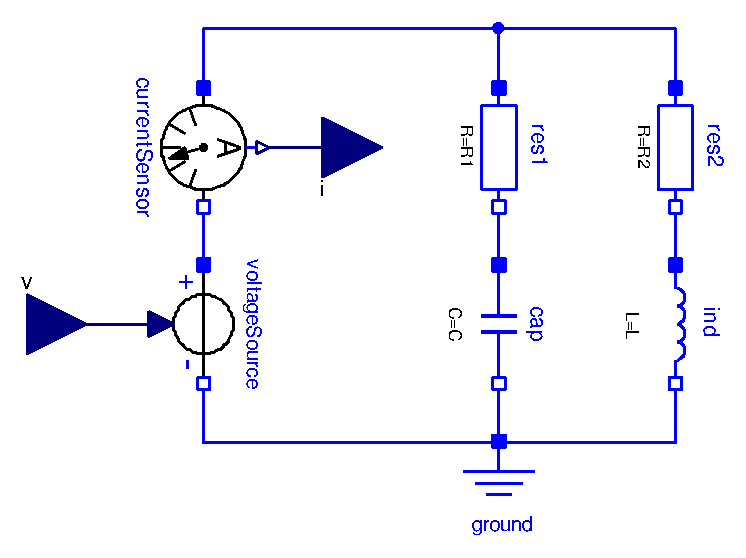
\includegraphics[width=0.6\linewidth]{1-Declarative-viD}%
    \label{fig:DeclarativeCircuit}%
  }\\
  \subfloat[Imperative]{
    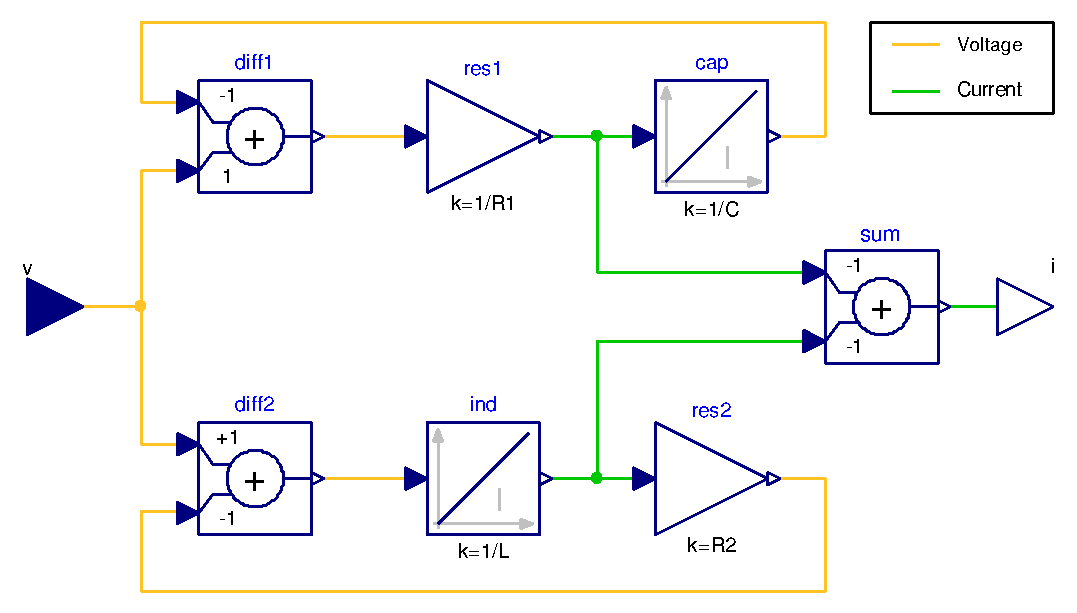
\includegraphics[width=0.8\linewidth]{1-Imperative-viD}%
    \label{fig:ImperativeCircuit}%
  }%
  \caption[Imperative and declarative models of an electrical circuit]{Imperative and declarative and imperative models of an electrical circuit~\cite{ModelicaTutorial1.4}}%
  \label{fig:Circuit}%
\end{figure}

\begin{figure}[htbp]
  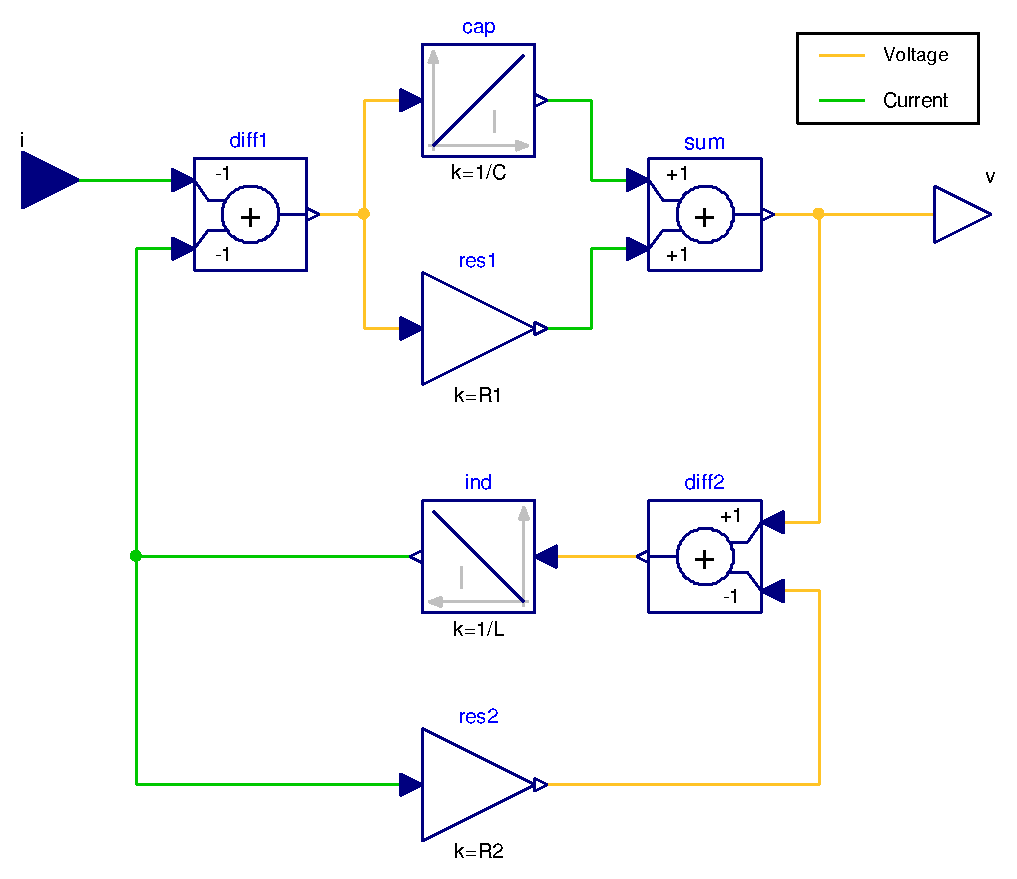
\includegraphics[width=0.8\linewidth]{1-Imperative-ivD}%
  \caption{Inverse imperative model of the circuit in \autoref{fig:Circuit}}%
  \label{fig:ImperativeCircuitInverse}%
\end{figure}

The fourth and final advantage of declarative models is that they are less prone to user error.  Some modeling mistakes may be avoided because the conservation laws are inherently and rigorously included.  If the developer of a model library uses the correct conservation equations in the lowest-level models, any circuit a user builds from the library is guaranteed to also include the correct conservation equations via Kirchhoff's current law, which is applied at every node.  In an imperative model, the conservation equations must be manually included at every level of the model; therefore, it is easier to violate conservation equations~\cite{Matei2012}.  In addition, a user may be tempted to cascade two instances of imperative models such as the ones in Figures~\ref{fig:ImperativeCircuit} and \ref{fig:ImperativeCircuitInverse}.  This is incorrect because the impedance of the second circuit affects the output of the first.  Two instances of the declarative model (\autoref{fig:DeclarativeCircuit}) can be easily and correctly cascaded by connecting the two in parallel (after removing the voltage source of the second instance).


\subsection{Current Limitations}
\label{sec:DeclarativeLimitations}

\N{EOO} or declarative, circuit-based modeling has been gradually extended from Kirchhoff's electrical circuit laws of 1845 to the magnetic, rotational, translational, thermal, fluid, and chemical domains.  In each domain, the \emph{\np{effort}} and \emph{\np{flow}}\glsadd{flow-adj}, or physical quantities analogous to voltage and current, are now well-established.  However, the fluid and chemical domains are more complicated because the material flow carries not only atoms or molecules but also significant amounts of other conserved quantities such as momentum and energy~\cite{Cellier2009}.  This process is called \emph{\n{advection}} and is depicted in \autoref{fig:Advection}.  By nature, the amount of these quantities depends on the source of the material.  Methods have been developed to use the property of the source by switching according to the direction of material flow (see \autoref{sec:Upstream}).

However, the switching approach has two drawbacks.  The first is that it generally requires reinitialization upon flow reversal.  This can usually be handled without a problem, but it requires additional computation.  In some cases there is chattering, or frequently repeated flow reversal, which can slow a simulation considerably.  The second drawback is that the intensive property is ill-defined when the material flow rate is zero.  This can be addressed by building a method of regularization into the switching algorithm.  This is of little immediate consequence because there is no advection at zero material flow rate.  However, it is at zero material flow rate that \emph{\n{diffusion}}, or transfer due to thermal activity with no net material flow, dominates.  Diffusion occurs towards lower values of the intensive property as depicted in \autoref{fig:Diffusion}.  Diffusion is not captured by the switching approach.

\begin{figure}[htbp]
  \subfloat[Advection]{
    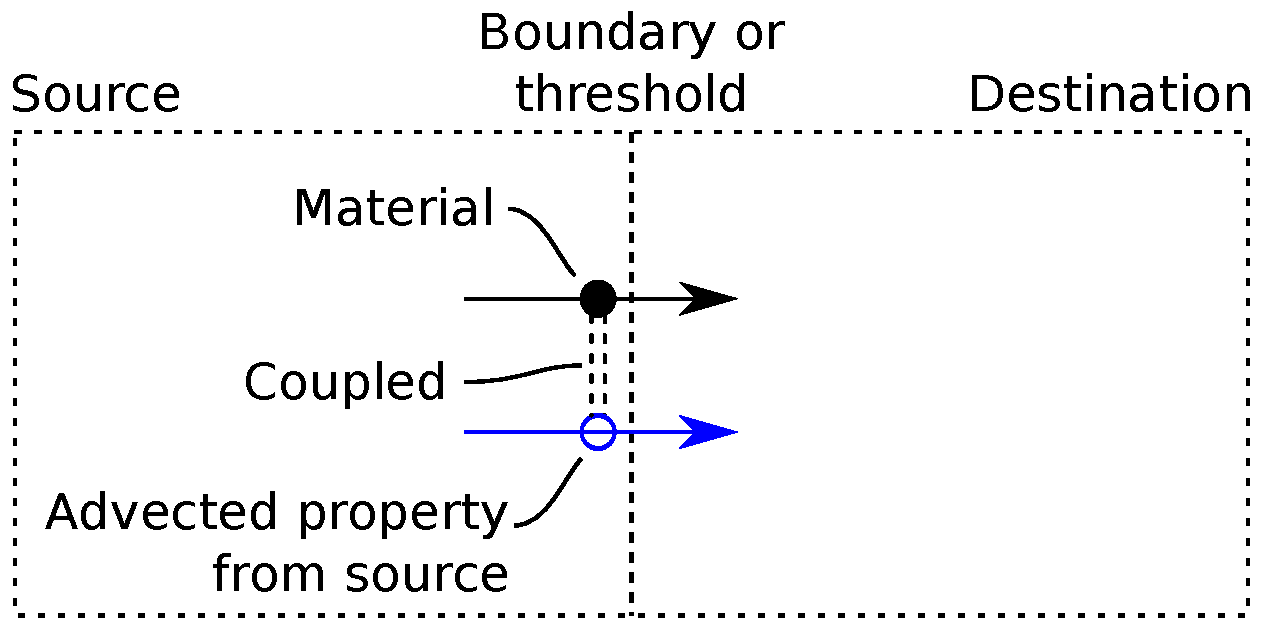
\includegraphics[width=0.48\linewidth]{1-Advection}%
    \label{fig:Advection}%
  }\quad
  \subfloat[Diffusion]{
    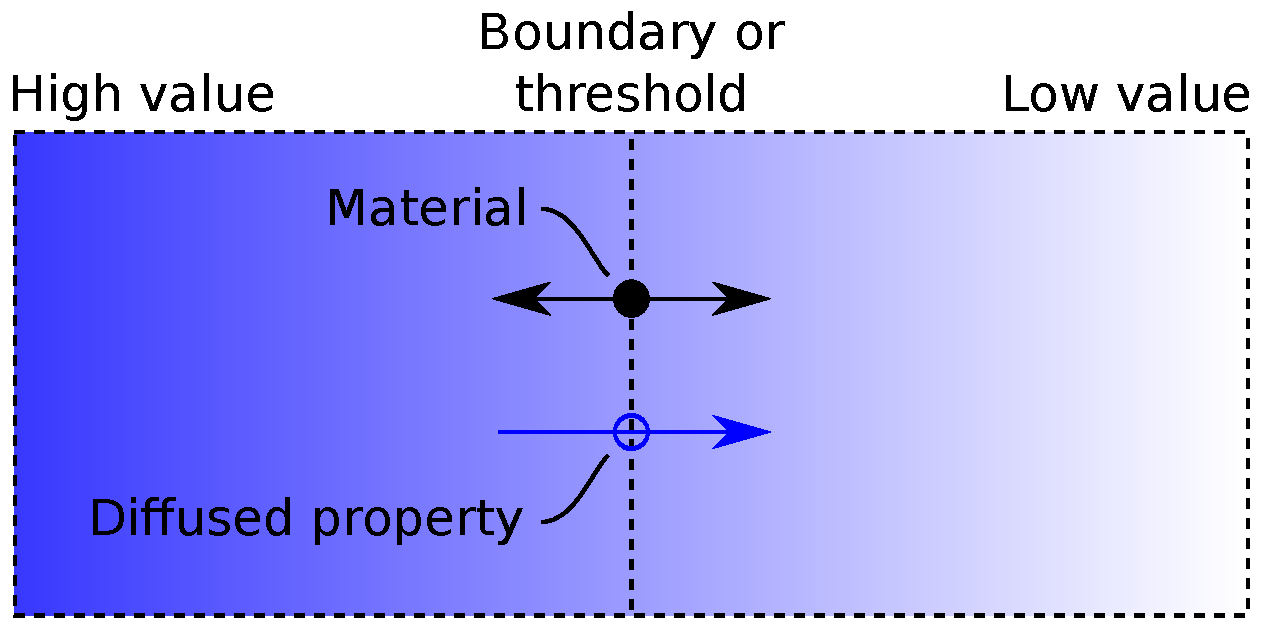
\includegraphics[width=0.48\linewidth]{1-Diffusion}%
    \label{fig:Diffusion}%
  }%
  \caption[Depiction of advection and diffusion]{Depiction of the two fundamental modes of transfer}%
  \label{fig:AdvectionDiffusion}%
\end{figure}

In some physical situations, there is mixed advection and diffusion.  To describe these situations, it is possible to add an additional pathway for purely diffusive transfer.  However, this is redundant and inconsistent because it yields two intensive properties at the boundary---one for advection and one for diffusion.  It also does nothing to eliminate the switching behavior or to resolve the advected property which is ill-defined at zero material flow rate.  This is the problem that the present research addresses---to model coupled advection and diffusion in a manner that is declarative, object-oriented, mathematically well-defined, numerically efficient, and physically representative yet generic.



\section{Research Questions}
\label{sec:Questions}

The goal of this research is to realize the advantages of declarative modeling for complex physical systems that involve both advection and diffusion to varying degrees in multiple domains.  We seek to answer the following questions:
\begin{enumerate}[\bfseries RQ1:]
  \item How can we create a generic declarative framework to model systems with processes that exhibit coupled advection and diffusion?
  \item How can the equations be best implemented to reflect the physical structure of a device and support reconfiguration?
  \item How appropriate is the framework for modeling all the relevant physical phenomena of an electrochemical device such as a fuel cell?
\end{enumerate}
The last question will be elaborated in the following section.



\section{Application to Fuel Cells}

In this dissertation, the modeling framework will be applied to fuel cells.  This will provide a pertinent and nontrivial demonstration of the framework while also establishing a novel approach to fuel cell modeling.  Declarative fuel cell models are physically appropriate~\cite{Zenith2006}, yet few models of this type exist (as shown in \autoref{chap:Background}).


\subsection{Context and Motivation}
\label{sec:FCMotivation}

\Np{FC} have the potential to serve a key role in our electric power networks, transportation systems, and portable electronic devices.  In general \np{FC} can convert fuel energy to work more efficiently and quietly than \np{ICE}~\cite{Larminie2003}, %[p.~23]
and a \n{FC} system's energy-to-power ratio can be easily adapted, unlike batteries.  A \n{FC} system can be refueled quickly like an \n{ICE} system, or it can be designed to recharge like a battery by operating in electrolysis mode~\cite{Burke2003}.  Of the various \nname{FC} technologies, \np{PEMFC} are best suited to meet the packaging and power-cycling requirements of vehicles and portable devices.

\Np{PEMFC} have a solid polymer-based electrolyte and operate at low temperatures (typically below \SI{100}{\celsius}).  As shown in \autoref{fig:CellFlows}, a single-cell \n{PEMFC} has few main components: a \n{PEM}, two catalyst layers or electrodes, two \np{GDL}, and two flow plates (FPs)~\cite{Larminie2003}. %[pp.~14--15 \& 67]
However, most applications require a higher voltage than a single-cell \n{PEMFC} can provide; therefore, two or more cells are joined back-to-back to form a \n{PEMFC} stack like the one shown in \autoref{fig:Stack}.

\begin{figure}[htbp]
  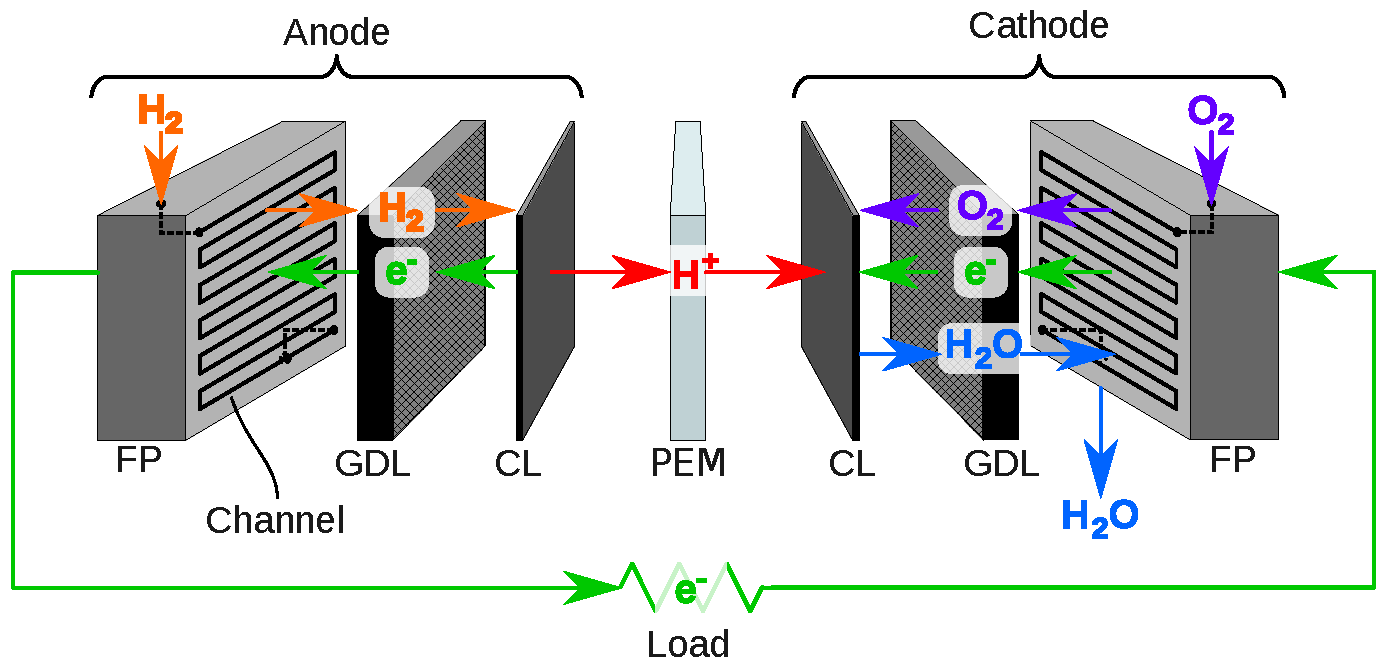
\includegraphics[width=0.75\linewidth]{1-CellFlows}%
  \caption[Layers of a single-cell \n{PEMFC}]{\glsreset{e-}%
  \glsreset{H+}%
  \glsreset{H2}%
  \glsreset{O2}%
  \glsreset{H2O}%
  Layers of a single-cell \n{PEMFC} and the primary paths of \n{e-}, \n{H+}, \n{H2}, \n{O2}, and \n{H2O} during normal operation}%
  \glsreset{e-}%
  \glsreset{H+}%
  \glsreset{H2}%
  \glsreset{O2}%
  \glsreset{H2O}%
  \label{fig:CellFlows}
\end{figure}

\begin{figure}[hbtp]
  \includegraphics[width=0.4\linewidth]{1-Stack}%
  \caption[\n{PEMFC} used to power an unmanned aerial vehicle]{\SI{500}{W}, 32-cell, water-cooled \n{PEMFC} used to power an unmanned aerial vehicle~\cite{Bradley2008}%[pp.\ 135--136]
}%
  \label{fig:Stack}
\end{figure}

A \n{PEMFC} operates on the chemical energy released by the reaction of \n{H2} and \n{O2} to produce \n{H2O}:
\begin{subequations}
  \begin{align}
    2\timessep\big(\s{H2} &\rightarrow 2\timessep\s{e-} + 2\timessep\s{H+}\big)\tag{HOR}\label{eq:HOR}\\
    4\timessep\s{e-} + 4\timessep\s{H+} + \s{O2} &\rightarrow 2\timessep\s{H2O}\tag{ORR}\label{eq:ORR}\\[-1.5em]
    \cline{1-2}\noalign{\vskip -0.9em}
    2\timessep\s{H2} + \s{O2} &\rightarrow 2\timessep\s{H2O}\tag{Net}\label{eq:CellReaction}
  \end{align}
\end{subequations}
Its \n{PEM} (electrolyte) controls the reaction by selectively passing protons while acting as a barrier layer to hydrogen, oxygen, and \n{e-}, as shown in \autoref{fig:CellFlows}.  This forces the reaction to occur in two sub-reactions:  the \n{HOR} whereby hydrogen is consumed and electrons and \n{H+} are produced, and the \n{ORR} whereby oxygen, electrons, and protons are consumed and water is produced.  In order to complete the full reaction, the electrons must travel an external path.  The path is provided by an external load which can harness the energy of the net reaction.

\glsunset{e-}
\glsunset{H+}
However, the cell has internal losses that cause heat generation and limit the rate at which the electrons can do a given amount of external work.  Some of the energy goes into making the reactions occur fast enough (activation losses), friction between the charge carriers (\n{e-} and \n{H+}) and the conducting materials (Ohmic losses), and transporting the reactants to and products away from the catalyst layers (concentration losses).

In order to operate, a \n{PEMFC} must be supported by other components, which are collectively called the \n{BOP}.  The \n{PEMFC} stack and \n{BOP} are the basis of a complete \n{PEMFC} system like the one shown in \autoref{fig:Ballard}.  \autoref{fig:FCSystem} shows the configuration of two \n{PEMFC} systems---one relatively simple and the other relatively complex.  Even more complex \n{PEMFC} systems may include heat recovery~\cite{Faghri2005} and fuel reformation.
\begin{figure}[htbp]
  \includegraphics[width=0.5\linewidth]{1-Ballard}%
  \caption[\n{PEMFC} system used to power a bus]{\SI{100}{kW} \n{PEMFC} system used to power a bus.  From Georgetown University, ``Generation III Project,'' \url{http://fuelcellbus.georgetown.edu}, accessed Nov.\ 2011%
}
  \label{fig:Ballard}
\end{figure}

\begin{figure}[htbp]
  \subfloat[Simple]{
    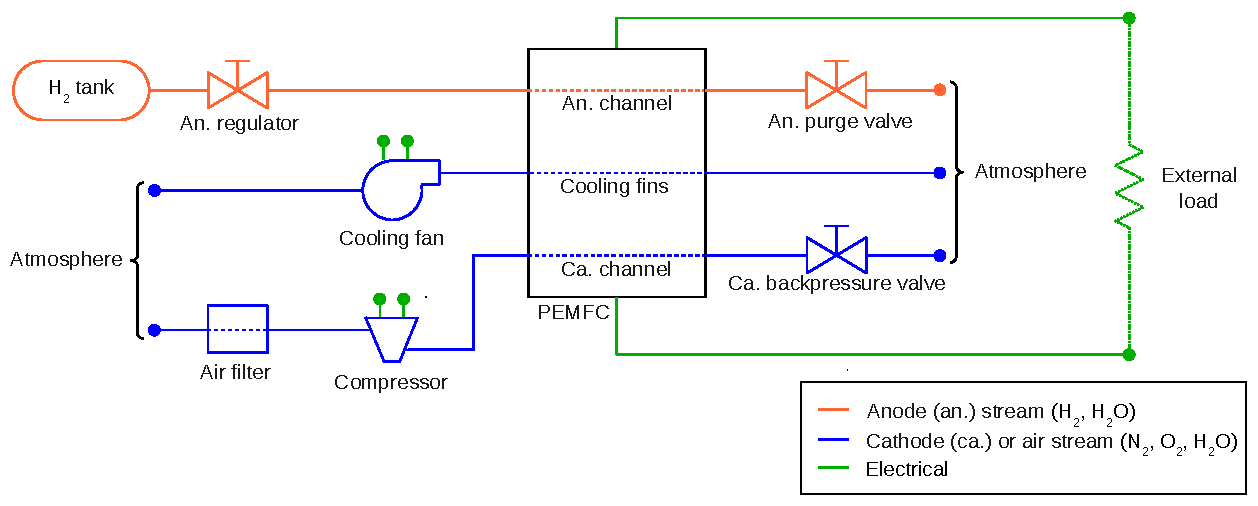
\includegraphics[width=0.75\linewidth]{1-SystemSimplest}%
    \label{fig:FCSystemSimplest}
  }\quad
  \subfloat[Complex]{
    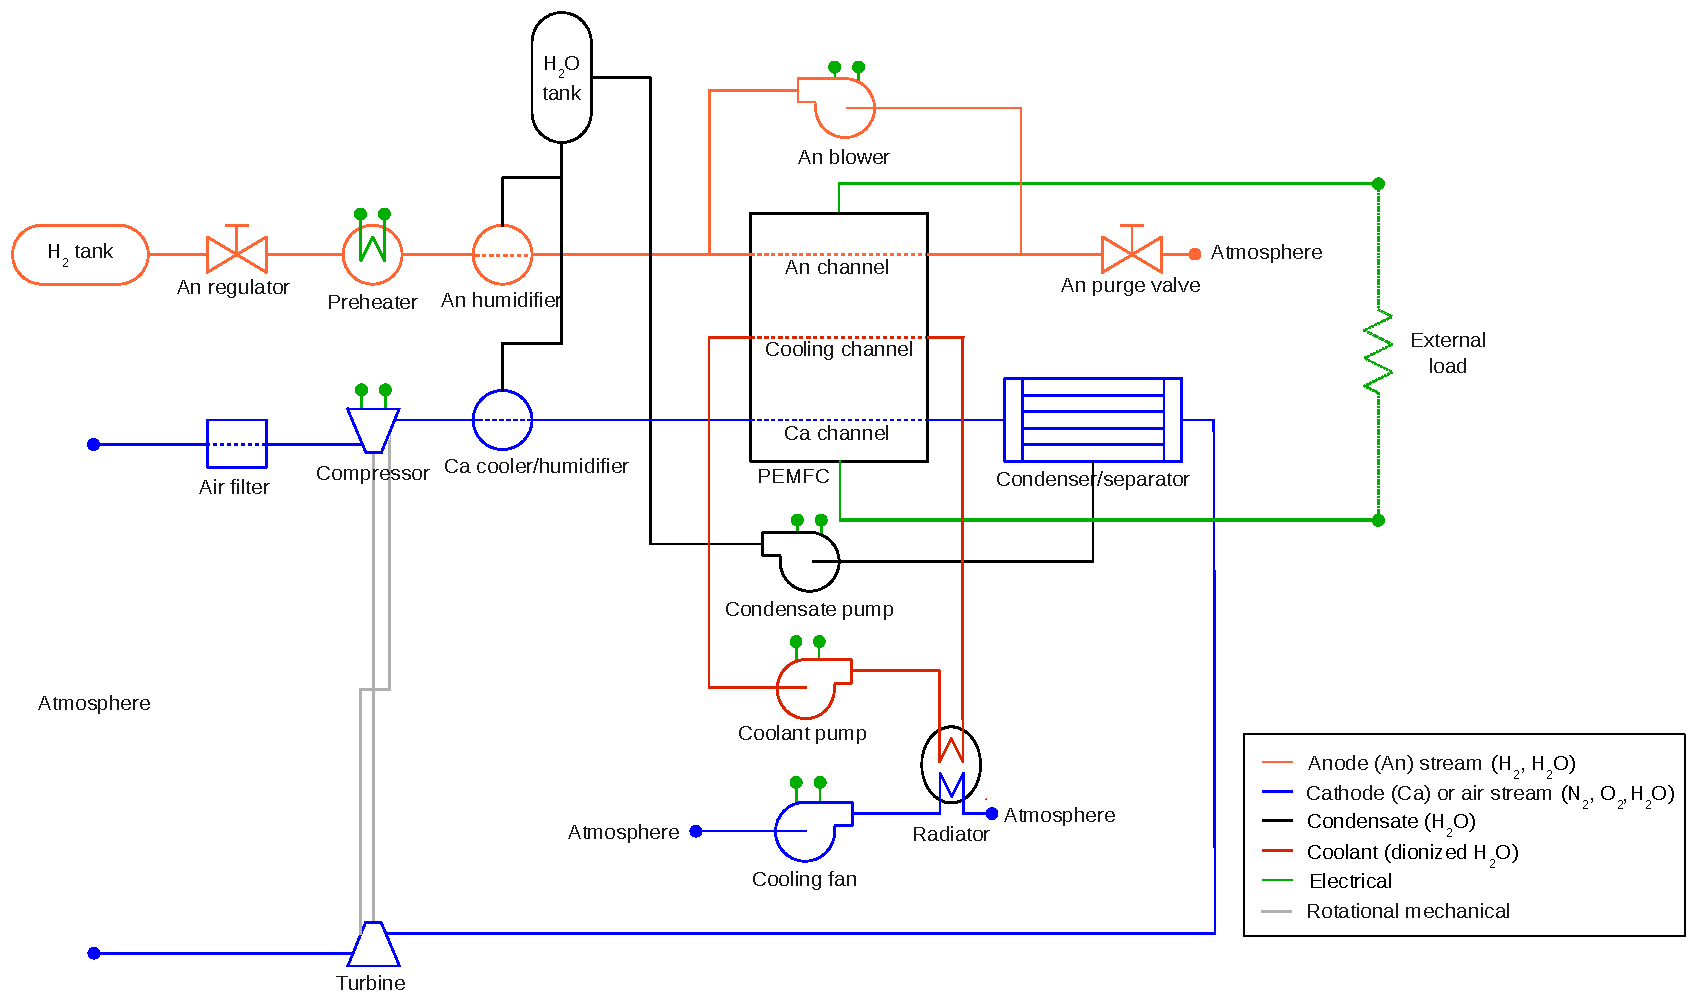
\includegraphics[width=\linewidth]{1-SystemComplex}%
    \label{fig:FCSystemComplex}
  }
  \caption[Configurations of two \n{PEMFC} systems]{Configurations of two hydrogen-fueled (non-reforming), pressurized \n{PEMFC} systems where \subref{fig:FCSystemSimplest} the stack is air-cooled and \subref{fig:FCSystemComplex} the stack is water-cooled, the anode is preheated and recirculated, the anode and cathode are both humidified, and the cathode exhaust is expanded through a turbine}
  \label{fig:FCSystem}
\end{figure}
\glsadd{an.}
\glsadd{ca.}

Although \n{PEMFC} systems are promising, their cost and durability, and to a lesser extent, size and weight, must be improved to meet the desired standards for commercialization \cite[p.~11]{DOE2007}.  The U.S.\ Department of Energy has outlined the numerous avenues that are being pursued to improve the \n{PEMFC}, \n{BOP} components, and \n{PEMFC} system as a whole~\cite{DOE2007}.  The physical mechanisms of \n{PEMFC} degradation and failure are being determined and characterized through experimental and model-based investigations \cite[pp.~3, 9, 32, \& 40]{DOE2007}.  Novel materials and structures are being identified and developed for the core components of a \n{PEMFC} (\autoref{fig:CellFlows}) as well as the seals between and around them \cite[pp.~4--7]{DOE2007}.  These efforts seek to lower the cost of materials, improve thermodynamic efficiency (by decreasing the activation, Ohmic, and concentration losses), and improve robustness (specifically to air and fuel impurities, temperature and humidity variations, corrosive conditions, and power cycling).   Design techniques and manufacturing processes are being developed to support the low-cost and high-throughput production of \np{PEM}, electrodes, and flow plates \cite[pp.~2, 5--6, \& 29--30]{DOE2007},~\cite{Ding2010}.   One goal is to more effectively integrate the \n{PEM} and electrodes (as a \nname{MEA}\glsreset{MEA}) in order to minimize interfacial resistances, while at the same time allowing the raw materials to be reused or recycled \cite[pp.~3--10]{DOE2007}.

The \n{BOP} components are being improved as well.  New materials and  concepts are being applied to heat exchangers, humidifiers, compressors, and turbines with the goal of reducing their size, weight, and cost \cite[pp.~7, 10, \& 32]{DOE2007}.  Since the air compressor places a significant internal electrical load on the \n{PEMFC} system, it is important to maximize its efficiency, and in some cases, a turbine is beneficial \cite[p.~102]{Larminie2003}.  Air filtration technology is being evaluated to allow \np{PEMFC} to be used in off-road applications.  Sensors, especially those for chemical composition, are being further developed for reduced cost and size and improved accuracy, reliability, durability, and dynamic response. \cite[pp.~7]{DOE2007}.  The design of reformers and the operation of \n{PEMFC} on reformate is also being improved \cite[pp.~8--9]{DOE2007}, but in applications fueled by hydrocarbons rather than hydrogen, \np{PEMFC} are less likely to be prevalent over high-temperature \n{FC} technologies that can accept those fuels directly (and perform internal
reformation).

The final area of work considers how to improve the \n{PEMFC} system as a whole.  Alternative \n{PEMFC} system configurations and design parameters are being considered that may allow the functions of the \n{PEMFC} system to be performed by fewer or simpler components, or that may entirely eliminate the need for certain functions \cite[p.~10]{DOE2007}.  For example, one of eight or more possible methods for external humidification may be chosen, or the \n{PEMFC} can be operated within certain ranges of temperature and air flow rate where external humidification is not necessary \cite[pp.~83--90]{Larminie2003}.  Such choices must be guided by sufficiently accurate information, so \np{PEMFC} are being tested to evaluate their performance, durability, and other properties under various operating conditions, including hydrogen impurity \cite[p.~9]{DOE2007}.

Mathematical models are used to assist many of these efforts to develop \np{PEMFC}.  These models offer several benefits.  First, the operating conditions of a model can (in theory) be adjusted and measured easily.  As stated by Cellier, ``in the simulation world, all inputs and outputs are accessible''~\cite{Cellier1991}.  This can help provide insight into working mechanisms of a fuel cell~\cite{Faghri2005} via techniques such as model-based data analysis~\cite{Matzopoulos2007}.  Second, simulations are perfectly repeatable.  Models are not subject to unidentified disturbances and measurement error.  This means, for instance, that the effects of a design parameter can be clearly identified.  Third, fuel cell models are faster and cheaper to run than test equipment~\cite{Faghri2005, Matzopoulos2007}.  This is very important in design exploration, where many tests must be performed.  It also allows extreme operating conditions to be tested without risking damage to the fuel cell hardware.  Fourth, fuel cell models can help to organize and share knowledge about the configuration of a fuel cell and its working principles \cite{Matzopoulos2007}.  This is particularly important since fuel cells are multi-physical devices that require multi-disciplinary research and development.

However, due to the complexity of the structures and the physical processes that occur within \np{PEMFC}, specialized models are typically required for different situations.  Many academic articles have been published with \n{PEMFC} models that are appropriate and useful for particular cell designs, operating conditions, and levels of fidelity (i.e., spatial, dynamic, or behavioral detail~\cite{Pyster2012}) %[p. 83]
\cite{Faghri2005}.\footnote{The next chapter contains a literature review.}  Ideally, variants of a common \n{PEMFC} model could be used for a wide range of research and development work, including physical investigation, model-based systems design, and model-based control.  Such a model library could offer an open framework for \n{PEMFC} researchers to contribute their expertise and benefit from the collective knowledge of others.

A broadly applicable \n{PEMFC} model library would need to contain models that are \emph{physically representative}, meaning their predictions of behavior match reality (i.e., \emph{accurate}) and their structure corresponds to the physical domain.  Specifically and at a minimum, the static voltage-current predictions should be accurate over the following ranges of operating conditions:
\begin{itemize*}
\item \SIrange{0.3}{0.9}{V} electrical potential difference (per cell)\footnote{Low cell potentials (high electrical currents) are avoided in order to reduce the chemical\slash{}electrochemical transport losses.  High cell potentials are avoided because they accelerate the corrosion that occurs due to electrical cycling \cite[pp.~6--7]{Schmittinger2008}.}
\item \SIrange{20}{80}{\celsius} temperatures of flow plates and inlet gases (all varied together)\footnote{The lower bound corresponds to start-up from room temperature.  Nafion, the most common membrane material, dehydrates above \SI{\sim80}{\celsius}, which increases its protonic resistance~\cite{Hallinan2010}.}
\item \SIrange{1}{3.5}{atm} absolute anode\slash{}cathode outlet pressures (varied together)\footnote{Some \np{PEMFC} operate at atmospheric conditions.  \n{PEMFC} system efficiency is unlikely to increase above a pressure ratio of ${\sim}3.1$ \cite[p.~107]{Larminie2003}}
\item 0\% to 100\% relative humidity at anode inlet\footnote{For simplicity, some \n{PEMFC} systems do not have humidifiers (0\%).  Other systems humidify the anode as much as possible without causing flooding to occur (up to 100\%).}
\item 30\% to 70\% relative humidity at cathode inlet\footnote{The lower bound (30\%) corresponds to the relatively extreme case of operating the \n{PEMFC} without humidification in the Sahara desert on an average day \cite[p.~78]{Larminie2003}.  The cathode supply is usually not saturated; flooding would occur since \s{H2O}~is also produced in the cathode.}
\item 14\% to 100\% mean inlet\slash{}outlet oxygen concentration in dry cathode gas\footnote{The lower bound corresponds to a stoichiometric ratio of 1.5.  The risk of starvation increases as the ratio approaches 1.0.  \np{PEMFC} are also operated on pure oxygen in applications such as \np{UUV}.}
\end{itemize*}
The \n{PEMFC} model library should approximate the dynamic voltage-current response of actual cells at nominal operating conditions and varying large-signal electrical currents (e.g.,~\cite{Wagner1998}). %[p.~3787, Figures~2b and 2c]
It should capture the operational effects of design parameters including component sizes and material properties (for hardware analysis and design) and should be capable of linearization (for control analysis and design).  It should be able to describe relevant phenomena including electrochemical reactions, chemical\slash{}electrochemical transport, heat transport, and heat generation.  It should also have variable fidelity so that it can be used for layer-, cell-, stack-, system-, or application-level simulations.  Finally, it should be modular, meaning it should be possible to interconnect its submodels in various ways to build larger models analogous to the physical hierarchy.  Unfortunately, no current \n{PEMFC} model library can provide these features, let alone over the required range of operating conditions.


\subsection{Research Questions}%
\label{sec:FCQuestions}

As stated in research question three (RQ3), we will investigate how appropriate the declarative advective\slash{}diffusive framework is for modeling all the relevant physical phenomena of a fuel cell.  The hypothesis is that the framework can be used to help establish a fuel cell model library that is physics-based, modular, reconfigurable, accurate, and leads to numerically efficient and robust models.  As discussed in the previous section, such a library would be a valuable tool for fuel cell research and development.  In order to answer RQ3, we will address the following subquestions:
\begin{enumerate}[\bfseries RQ3a:]
  \item For which processes is it necessary to model mixed advection and diffusion?  Where is it appropriate to assume pure advection or pure diffusion?
  \item What characteristics do the models exhibit that would not be present given an imperative formalism?
  \item Which combinations of accuracy and speed can be achieved by adjusting fidelity?
\end{enumerate}



\section{Overview of the Modeling Approach}%
\label{sec:ModelingApproach}

As mentioned previously, the modeling approach is declarative, modular, and hierarchical.  This approach is also called \n{EOO} modeling.  The \autoref{fig:ModelHierarchy} illustrates that the models are created by building species (e.g., \s{H2}) into phases such as gas, phases into subregions, subregions into regions such as a fuel cell layer, and regions into assemblies such as a fuel cell.  This reflects the physical architecture of the device.
\begin{figure}[htbp]
  \newcommand{\I}[1]{\fbox{\includegraphics[height=2cm]{#1}}}
  \newcommand{\arrow}{\vbox to 1.95cm {\vfil
    \hbox{\LARGE $\rightarrow$}
    \vfil}}
  \I{4-SpeciesI}~\arrow~\I{4-PhaseI}~\arrow~\I{4-SubregionI}~\arrow~\fbox{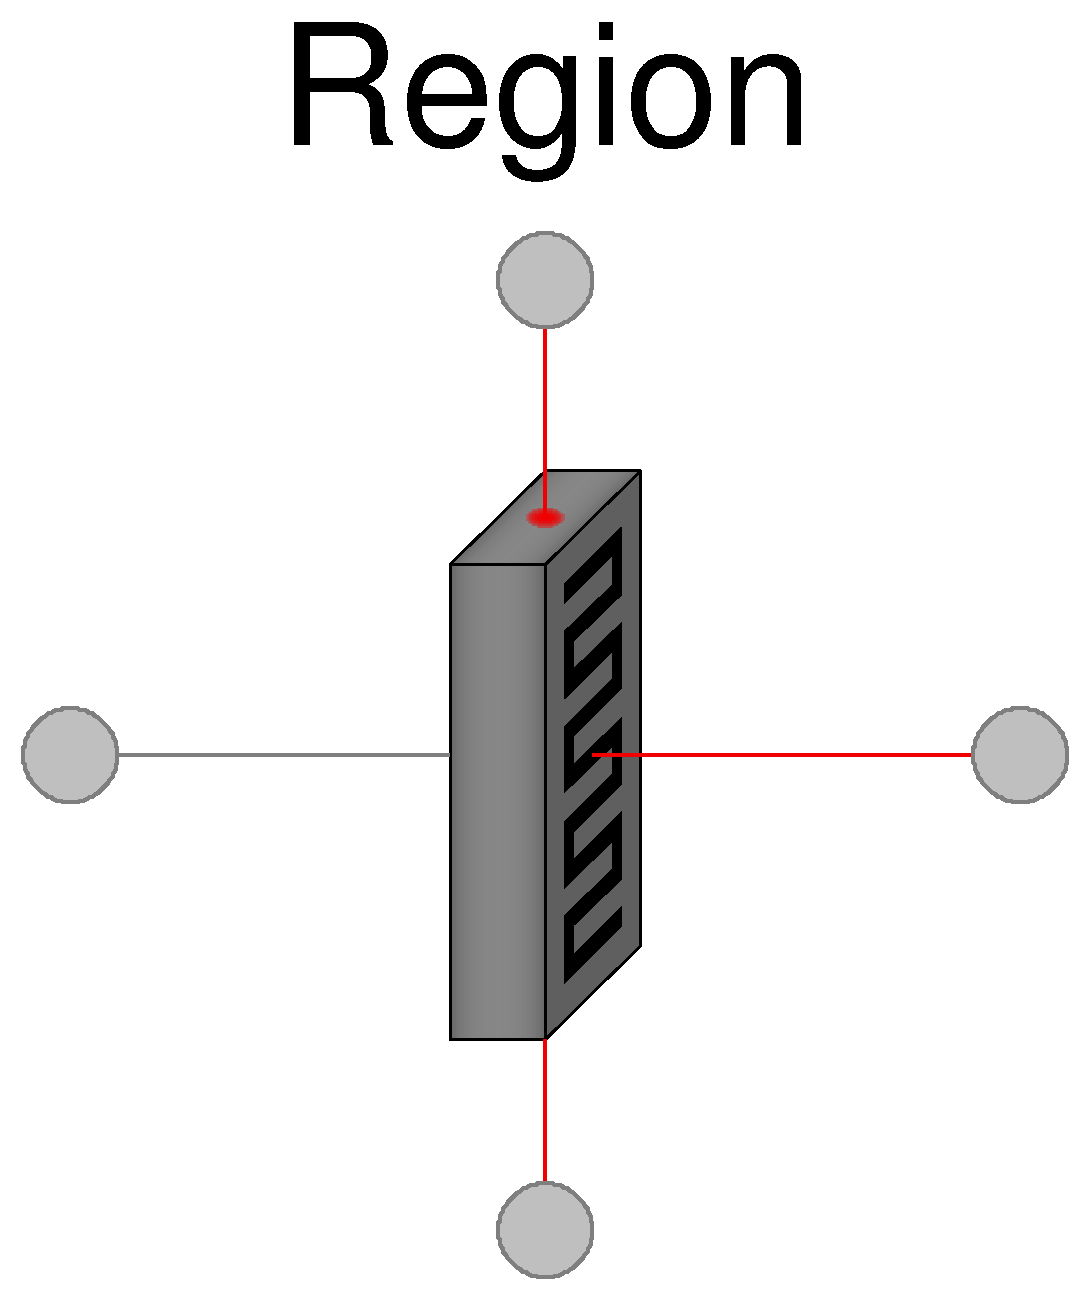
\includegraphics[height=2.4cm]{4-RegionI}}~\arrow~\I{4-AssemblyI}%
  \caption{Levels of physical hierarchy in the model library}%
  \label{fig:ModelHierarchy}%
\end{figure}

The models are highly reconfigurable.  Assumptions may be applied that affect the spatial resolution and the included species, phenomena, axes of material translation, and boundaries.  With each assumption, the number and complexity of the equations scale appropriately and without simulation overhead.  The characteristics of individual species are provided in replaceable packages.  The packages can be used to model incompressible and compressible fluids including ideal and real gases.  The thermodynamic properties and other correlations are adjusted automatically according to these assumptions.

The models are dynamic and continuous in time.  Transients are modeled in terms of \np{DAE}, or implicit \np{ODE} combined with algebraic constraints.  These \np{DAE} are implemented in the Modelica language~\cite{Modelica3.3}.

The models are discrete in space.  As stated by Mattiussi~\cite{Mattiussi2000}, %[pp.~2--3]
this representation has three advantages: \begin{inparaenum}[(1)]\item it provides a unified perspective that is appropriate for many theories, \item it directly correlates the discretization of the physical region and the structural properties of the applied theories, and \item it is based on intuitive geometrical and physical concepts that help distinguish the numerical methods (e.g., \n{FDM}, \n{FVM}, and \n{FEM}) and the underlying theories\end{inparaenum}.  Rather than implementing approximations to traditional \n{PDE} representations, the approach is to distill the key concepts from equations such as Navier-Stokes and formulate them in a manner best uses features of \n{EOO} language.  The models have options for one, two, or three dimensions.  The grid of control volumes is rectilinear but the lengths are adjustable.

Computational efficiency is emphasized.  The translated models contain only linear systems of equations.  Techniques are used to reduce computational complexity, for example by representing high-order polynomials in nested form.  Many optional assumptions may be enabled to simplify the model.  For example, the temperature of different phases may be constrained to be the same; this results in index reduction and a simpler model.

The advective\slash{}diffusive framework is applied to the electrical, thermal, fluid, and chemical domains.  The approach is deeply physics-based.  It employs dynamic conservation equations for material, translational momentum, and energy.  Since the models are also resolved down to the species level, this requires traditional equations to be described at a more fundamental level.  For instance, Ohm's law and the Maxwell-Stefan equations for multi-component diffusion are not implemented directly.  Instead, drag interactions are modeled in a manner that results in those equations.



\section{Outline of the Dissertation}
\label{sec:Outline}

In this chapter, we have introduced the research by discussing the motivation, questions, and general approach.  The subjects of the remaining chapters are as follows:
\begin{itemize*}
  \item \textbf{\autoref{chap:Background} --- \nameref{chap:Background}:}  Survey of the relevant literature in the areas of declarative modeling languages, approaches to fluid flow in declarative language, and fuel cell models
  \item \textbf{\autoref{chap:Fundamentals} --- \nameref{chap:Fundamentals}:}  Detailed presentation and justification of the model equations which cover thermodynamics, material properties, transport, and exchange
  \item \textbf{\autoref{chap:Implementation} --- \nameref{chap:Implementation}:}  Summary of the implementation of the equations in a fuel cell model library
  \item \textbf{\autoref{chap:Basic} --- \nameref{chap:Basic}:}  Discussion of the conditions and results of several low-level demonstrations of the model library
  \item \textbf{\autoref{chap:Cell} --- \nameref{chap:Cell}:}  Discussion of the conditions and results of polarization tests and a dynamic example of the fuel cell model
  \item \textbf{\autoref{chap:Conclusions} --- \nameref{chap:Conclusions}:}  Recapitulation of the dissertation, list of contributions, and suggestions for future work
  \item \textbf{\autoref{chap:RelatedTheory} --- \nameref{chap:RelatedTheory}:}  Derivations and discussions that relate the model to selected theories in fluid dynamics and solid-state physics
  \item \textbf{\autoref{chap:Doc} --- \nameref{chap:Doc}:}  User documentation, diagrams, source code, and tables of parameters and connectors of the fuel cell model library
\end{itemize*}

  \chapter{Background}
  \label{chap:Background}
  \glsresetall


In this chapter, we will review the literature and current developments in several related areas.  First, we will consider the \n{EOO} languages that are candidates for demonstrating the modeling contributions of this dissertation (\autoref{sec:EOOLanguages}).  Then we will describe the recent work to model fluid and chemical systems using the Modelica language in particular (\autoref{sec:Upstream}). Finally, we will review models of \glsreset{PEMFC}\np{PEMFC} with an emphasis on the modeling formalism (\autoref{sec:FCModels}).


\section{Equation-Based, Object-Oriented (EOO) Modeling Languages}
\label{sec:EOOLanguages}

There are five major domain-neutral, \n{EOO} modeling languages in current use and development:  Modelica, VHDL-AMS, Verilog-AMS, gPROMS, and Simscape.  A brief overview of these languages is given in the following sections.  All the languages support \np{DAE} and conservation equations via the generalized Kirchhoff current law.  The differentiation is in their syntax, semantics, additional features, and available model libraries and tools.  Since syntax and semantics are somewhat subject to preference, we will focus only on the features and the available libraries and tools.

Modelica, VHDL-AMS, and Verilog-AMS are standardized and tool-neutral, meaning that they are supported by multiple vendors whose software should operate on the same models.  This can help to prevent tool lock-in, or dependence on a particular vendor.  It also tends to encourage a community of open-source model developers.  The languages of gPROMS and Simscape are proprietary and integral to the modeling platforms of the same name by Process Systems Enterprise Limited and The MathWorks Inc., respectively.

In addition to the major domain-neutral \n{EOO} modeling languages, there are several languages that offer capabilities or approaches that are not yet mainstream.  Sol is a domain-neutral \n{EOO} language that is based on Modelica and supports variable-structure systems~\cite{Zimmer2010}.  This is important, for example, in mechanics where connections may be made or broken during the course of a simulation.  Hydra is the most mature language that uses \n{FHM}~\cite{Broman2010}.  This approach is based on functional programming languages such as Haskell.  Functional programming is a method of declarative programming, so it is naturally appealing for declarative or equation-based modeling.

Many other languages and platforms exist that are not simultaneously equation-based, object-oriented, and domain-neutral.  Languages such as Hybrid~$\chi$ and ASCEND are declarative but do not yet support declarative or acausal connections~\cite{Broman2010}.\footnote{This aspect of ASCEND is discussed at \url{http://www.ascend4.org/ascend_processmodeling.htm} (accessed Aug.\ 24, 2013).}  Engineering Equation Solver (EES; by F-Chart Software, LLC) is a declarative modeling tool that has an extensive thermodynamics library, but it does not support declarative connections either.  Numerous languages and platforms are declarative but are domain-specific---for example, aspenOne (Aspen Technology Inc.) for chemical process simulations.

The background of Modelica and Simscape is more general and multi-physical than VHDL-AMS, Verilog-AMS, and gPROMS\@.  Although all five languages are neutral with respect to physical domains, the history is important because it has implications on the extent of the user base and the depth and breadth of the available tools and model libraries.  \autoref{tab:Languages} lists the absolute and relative numbers of articles that reference the languages in four major scientific and engineering databases: Compendex and InSpec (\url{http://www.engineeringvillage.com/}), ScienceDirect (\url{http://www.sciencedirect.com/}), and Web of Science (\url{http://apps.webofknowledge.com/}).  In addition, relative internet search interest is listed from Google Trends (\url{http://www.google.com/trends/}).  Modelica appears to dominate these indices; the smallest margin (12\%) is with gPROMS in ScienceDirect.
% \url{http://www.google.com/trends/explore?q=vhdl-ams#q=Modelica%2C%20gPROMS%2C%20VHDL%20AMS%2C%20Verilog%20AMS%2C%20SimScape&date=1%2F2008%2049m&cmpt=q}

\captionsetup[table]{textformat=simple}
\begin{table}[hbtp]
  \caption[Relative occurrence of declarative modeling languages]{Relative occurrence of declarative modeling languages.\footnotemark}
  \label{tab:Languages}
  \begin{tabular}{l rrr rr rrr rrr rrr}
    \toprule
     & \multicolumn{3}{c}{\textbf{Compendex}} & \multicolumn{2}{c}{\textbf{InSpec}} & \multicolumn{3}{c}{\textbf{ScienceDirect}} & \multicolumn{3}{c}{\textbf{Web of Science}} & \multicolumn{3}{c}{\textbf{Google Trends}} \\
    \textbf{Name} & \multicolumn{3}{c}{\textbf{2013}} & \multicolumn{2}{c}{\textbf{2013}} & \multicolumn{3}{c}{\textbf{2013}} & \multicolumn{3}{c}{\textbf{2013}} & \multicolumn{3}{c}{\textbf{2008--2013}} \\
    \cmidrule(lr){2-4} \cmidrule(lr){5-6} \cmidrule(lr){7-9} \cmidrule(lr){10-12} \cmidrule(lr){13-15}
    & \# & Rel.\ && \# & Rel.\ & \# & Rel.\ && \# & Rel.\ && --- & Rel.\ \\
    \midrule
    Modelica & 108 & 66\% && 36 & 55\% & 112 & 48\% && 42 & 64\% && 74 & 63\% \\
    VHDL-AMS & 22 & 13\% && 10 & 15\% & 15 & 6\% && 9 & 14\% && 11 & 9\% \\
    Verilog-AMS & 4 & 2\% && 6 & 9\% & 9 & 4\% && 2 & 3\% && 3 & 3\% \\
    gPROMS & 11 & 7\% && 3 & 5\% & 84 & 36\% && 7 & 11\% && 13 & 11\% \\
    Simscape & 18 & 11\% && 10 & 15\% & 13 & 6\% && 6 & 9\% && 17 & 14\% \\
    \bottomrule
  \end{tabular}
\end{table}
\captionsetup[table]{textformat=period}


\subsection{Modelica}

Modelica~\cite{Modelica3.3} was designed as a ``multi-formalism, multi-domain, general-purpose modeling language''~\cite{Elmqvist1997}.  The designers sought to unify the basic syntax and semantics of many modeling languages that were present in the late 1990s, including Dymola, Omola, NMF, SIDOPS+, Smile, ObjectMath, \nobreak{ASCEND}, and U.L.M.~\cite{Elmqvist1997, Astrom1998}.  Of these, gPROMS, VHDL-AMS, and \nobreak{ASCEND} are still independently active.  Dymola is now a modeling and simulation tool that supports Modelica.

\footnotetext{The percentages have been rounded and may not add to 100\%.}

The Modelica language specification is still evolving with new releases every year or two.  It includes keywords and operators for discrete as well as continuous systems.  Methods have been proposed to support \np{PDE}~\cite{Fritzson2004, Saldamli2006}, but they have not yet been integrated into the language~\cite{Modelica3.3}.  Meanwhile, an imperative block-based library is available that uses the \n{MOL} or the \n{FVM} to convert parabolic or hyperbolic \np{PDE} to \np{ODE}~\cite{Dshabarow2007, Dshabarow2008}. \footnote{Available as the PDELib package at \url{https://github.com/modelica-3rdparty/PDELib}.}

% \cite{Saldamli2006}
% - Language level
% - define complex boundaries
% - apply causality
% Also explained at \url{https://www.ida.liu.se/labs/pelab/modelica/pde.shtml}

% Dshabarow2008 - good discussion of history and trends in PDE solvers and Modelica
% - limited to time-dependent problems
% FORSIM VI reimplemented in Modelica
% PDELib can use upstream discretization

% Li2008 (``Description of PDE Models in Modelica,'' ``Solving PDE Models in Modelica''):
% Exclude this
% - Doesn't even properly cite the previous work of Dshabarow and Saldamli
%   - Is it a copy of their work without attribution?
% - Implies that gPROMS is limited to PDEs over rectangular domains
%   - But Oh1996 does discuss parameterized boundaries in gPROMS

Modelica is supported by a growing number of software tools including Dymola (Dassault Syst\`emes), SystemModeler (Wolfram Research), MapleSim (MapleSoft), AMESim (Siemens AG), CyModelica (CyDesign Labs), SimulationX (ITI GmbH), and MWorks (Suzhou Tongyuan).  In addition, there are free modeling and simulation environments including OpenModelica (Open Source Modelica Consortium) and JModelica (Modelon AB).

Modelica has more than thirty free, open-source libraries contributed by the user community.\footnote{See \url{https://modelica.org/libraries}.}  The Modelica Association maintains the Modelica Standard Library, which contains well-established packages of thermal, fluid, electrical, magnetic, and mechanical components.  It also contains a package of thermodynamic and transport properties.


\subsection{VHDL-AMS}

VHDL-AMS is the combination of VHDL, a modern hardware description language, and extensions for analog and mixed signals.\footnote{VHDL-AMS stands for \underline{v}ery-high-speed integrated circuit (VHSIC) \underline{h}ardware \underline{d}escription \underline{l}anguage with \underline{a}nalog and \underline{m}ixed-\underline{s}ignal extensions.}  Whereas \np{HDL} have been used to describe the behavior of physical devices and processes since the 1960s, modern \np{HDL} also describe the structure of the device.  VHDL itself is an equation-based language for digital circuits in discrete time with events~\cite{Christen1999}.

The analog and mixed signal extensions are not specific to the electrical domain~\cite{Christen1999, VHDLAMS2007}.  However, due to the history of VHDL, the extensions are particularly appealing in cases where it is desirable to incorporate a model of the physical system with a digital circuit (e.g., an \n{ASIC}).


\subsection{Verilog-AMS}

Verilog-AMS parallels VHDL-AMS in many aspects.  VHDL and Verilog are both \np{HDL}, and both have been extended for analog and mixed signals.  Verilog-AMS was developed and is maintained by the Accellera consortium~\cite{VerilogAMS2.3.4} but has not yet been standardized by IEEE like VHDL-AMS\@.  Verilog-AMS does not support replaceable or encapsulated models like Modelica and VHDL-AMS~\cite{Pecheux2005}.  The equations in an analog block of Verilog-AMS must be manually sorted, and implicit equations are not entirely supported~\cite{Pecheux2005}.  P\^echeux et al.~\cite{Pecheux2005} compare Verilog-AMS and VHDL-AMS in detail.


\subsection{gPROMS}

The gPROMS\footnote{gPROMS stands for \underline{g}eneral \underline{pro}cess \underline{m}odeling \underline{s}ystem.} language was created in 1992 to support combined discrete\slash{}continuous systems~\cite{Barton1992}.  Several years later it was extended for partial differential equations using the \n{MOL}~\cite{Oh1996}.  gPROMS is now a commercial product of Process Systems Enterprise (PSE).

The gPROMS software suite is primarily marketed and applied to chemical process modeling~\cite{Broman2010}.  It has built-in tools for parameter estimation.  There are various add-on modules and libraries for chemical\slash{}physical properties and advanced components.  A fuel cell model library is also available.\footnote{See \url{http://www.psenterprise.com/gproms/aml/fc} (accessed Aug. 24, 2013).}


\subsection{Simscape}

Simscape~\cite{Mathworks2012, SimPowerSystems5} extends the Simulink control systems platform with support for physical system simulation.  The Simscape language is a relatively new offering from The Mathworks Inc.\ (October 2008)~\cite{MathWorks2008} and is likely the company's response to the predominance of Modelica.  Its syntax is somewhat similar to Modelica but is not based on an open standard.  Simscape includes libraries of mechanical, electrical, thermal, and hydraulic components which are similar in concept to those of the Modelica Standard Library.  However, they are integrated with the product rather than freely available.


\section{Fluid\slash{}Chemical Modeling in Modelica}
\label{sec:Upstream}

Much of the literature in fluid dynamics and mass transfer uses \np{PDE}, but the core formalism of \n{EOO} models is differential algebraic.  \np{PDE} may be introduced by extensions to the \n{EOO} language (e.g., gPROMS~\cite{Oh1996}) or model libraries (e.g., Modelica~\cite{Modelica3.3}); however, the capabilities are limited compared to languages and tools that are designed primarily for \np{PDE} (e.g., OpenFOAM or COMSOL).  Thus, it may be best to implement analytical solutions or correlations to experiments or offline \n{CFD} simulations where possible.  Co-simulation is also becoming a strong option with the movement towards software interoperability (e.g., the \nname{FMI}---FMI).  However, in using co-simulation (as well as \n{PDE} extensions or libraries in an \n{EOO} environment), it is important to weigh the value of increased fidelity against the computational requirements of distributed submodels in an otherwise lumped-parameter model.

Given the current limitations of including \np{PDE} in an \n{EOO} environment and the conceptual advantages of discrete-space representations (see \autoref{sec:ModelingApproach}), the following survey is limited to \n{DAE}-compatible representations of fluid and chemical systems.  It is also limited to the Modelica language, since it offers the largest base of open-source work in the area.  The discussion emphasizes advection and diffusion since they are central to fluid and chemical models.  A common theme is how the one-way nature of advection is handled given the two-way nature of equations and declarative language.  %In terms of differential equations, this type of problem is classified as parabolic~\cite{Patankar1980}.  In \np{DAE}, it is often addressed by an implementation the upwind scheme.

% McGill University investigation into distributed heat flow in Modelica.


\subsection{Without Coupled Advection}


The easiest approach to modeling fluid\slash{}chemical systems is to ignore the advection of properties with the material stream.  In some physical situations, this is appropriate because the advection of momentum and energy is insignificant and the material flow is purely advective or diffusive.  For example, in chemical diffusion, the material flow may be slow enough that the rates of advection of momentum and energy are negligible or are dominated by translational and thermal diffusion (i.e., friction and thermal conduction).\footnote{As presented in \autoref{chap:Fundamentals}, purely diffusive material flow can cause thermal advection.  It should be noted that thermal convection is thermal conduction in series with thermal advection.}  These assumptions are implicit in the BioChem~\cite{Nilsson2003, Nilsson2005} and ADGenKinetics~\cite{Elsheikh2012} biochemical libraries.  Their connectors only consist of concentration as an effort variable and molar flow rate or volumetric reaction rate (respectively) as a flow.  In isothermal, isochoric, pressure-driven scenarios (e.g., simple pipe flow), there is no material diffusion.  Heat transport may not be of interest, and the rate of momentum transport (dynamic pressure times area) is proportional to the square of the rate of material advection.  Then it is only necessary to include the pressure and material (or mass) flow rate at each boundary.  This is the case in pure hydraulics (e.g., the OpenHydraulics library in Modelica~\cite{Paredis2008}).  It is also essentially the case for electrical circuits, where electrical conduction (a la Ohm's law) is actually material advection (of charge carriers).  %It is interesting that the model equations have the same form in the purely diffusive case (e.g., Fick's law) and the purely advective case (e.g., Poiseuille's law or Ohm's law).


\subsection{Central Difference}

Another approach is to include advection but ignore its one-way nature.  This is the essence of the central difference scheme.  It can be accomplished in an \n{EOO} framework by adding a diffusive pathway for the appropriate quantities (e.g., energy) to determine properties such as temperature at a boundary.  If the resistances to either side of a boundary are equal, then the value of a property at the boundary is the mean of the values in the neighboring subregions, just as it is in the central difference scheme.  Advection can then be determined using the mean value.

Unfortunately, the central difference scheme gives unrealistic results when the rate of advection is large compared to the rate of diffusion~\cite{Patankar1980}. %[pp.\ 82--83]
 It is generally accepted that some form of upstream discretization is necessary, and current Modelica libraries do not use the central difference scheme for fluid flow.



\subsection{Without Coupled Diffusion}
\label{sec:NoDiffusion}


The third approach is to assume that the advection is not accompanied by any diffusion.  If there is no diffusion, then the advected property only depends on the material source(s).  This is the upwind scheme, also known as the upwind-difference scheme, the upstream-difference scheme, or the donor-cell method~\cite{Patankar1980}.  Unfortunately, the upwind scheme implies causality which is difficult to implement in declarative or acausal language.  It introduces challenges with respect to \begin{inparaenum}[(1)]\item the semantics of the language and \item the numerical robustness and computational efficiency under initialization, zero material flow, and flow reversal\end{inparaenum}.  These challenges have led to a number of sub-approaches, which are described in the following sections.

Due to the assumption that the advected properties are not affected by diffusion, this approach is more appropriate for fluid networks than for chemical devices.  Diffusion could be added in parallel with the advective flow, but as mentioned in \autoref{sec:DeclarativeLimitations}, this would produce redundant and inconsistent intensive properties at a boundary.


\subsubsection{Balanced Efforts and Flows}
\label{sec:BalancedEffortFlow}

One sub-approach, embodied by the \modelica{semiLinear} function of Modelica, is to implement the upwind scheme using pairs of effort and flow variables~\cite{Elmqvist2003}.  This is appealing because the effort\slash{}flow construct is well-established in \n{EOO} languages and supports an arbitrary number of connections at a node.  The advected property is like an effort in that it is equal among the connected models.  It can be calculated from the generalized Kirchhoff current law for the associated flow variable.

The value of the advected property depends on the material source(s), so it is discontinuous upon reversal of the material or mass flow.  This is not generally a problem, but difficulties arise when the material or mass flow rates are zero or are not explicitly known.  If the mass flow rates are zero, then the effort variable (the advected property) disappears from the system of connection equations---a mathematical singularity.  If the mass flow rates are not known, they must be solved from the connection equations.  This is challenging because it is a nonlinear problem with Boolean expressions (the upwind conditions)~\cite{Franke2009}.


\subsubsection{Special Connectors}
\label{sec:SpecialConnectors}

Other implementations add special variables to the connectors besides the primary effort\slash{}flow pair for material or mass transport.  The conservation equation associated with the advected property is instantiated multiple times for each node.  This is in contrast with the balanced effort\slash{}flow approach (previous section), where there is one conservation equation for every node---the generalized Kirchhoff current law.

The standard approach in the Modelica language since version 3.1 (May 2009) is to use a connector where the \modelica{stream} keyword denotes a property which is advected with the material.  This property is not an effort or a flow, and in fact, it is not equal among connectors at a node.  A stream connector contains one driving property such as pressure, one flow variable such as mass flow rate, and one or more stream properties.  Model equations can reference a stream property directly or via built-in \modelica{inStream} or \modelica{actualStream} operators.  A direct reference yields the value of the property that would hypothetically occur if material is exiting a component.  The \modelica{inStream} operator returns the value that would occur if material is entering the component.  The \modelica{actualStream} operator returns the actual value which depends on the flow direction~\cite{Modelica3.3}.

This organization avoids the need to devote a variable to the actual, mixed value of the advected property.  As mentioned previously (\autoref{sec:BalancedEffortFlow}), that value is ill-defined at zero-flow conditions and discontinuous upon flow reversal.  With the \modelica{actualStream} operator, it is determined only where it is needed, for example in the conservation equations of control volumes and in the definitions of variables for analysis and plotting.  In the conservation equations, it is multiplied by the material or mass flow rate such that the product is not discontinuous~\cite{Modelica3.3}.  In other cases, either the outflow value (direct reference to the stream variable) or the inflow value (\modelica{inStream} operator) is appropriate.  The outflow value usually depends on the thermodynamic state of a control volume (no Boolean conditions) or on inflow value(s).  The inflow value is calculated from a unique conservation equation for each connector given the assumption that fluid is entering the associated component.  Although the actual material or mass flow rates of the other connectors are used in the equation, this means fewer discontinuities~\cite{Franke2009}.  The Modelica specification requires that modeling tools implement a method of regularization to eliminate the singularities at zero material flow~\cite{Modelica3.3}.  However, since stream connectors are a relatively new addition to the Modelica language, some modeling tools do not fully support them.

The Modelica Fluid library, which is part of the Modelica Standard Library, uses stream connectors to model \nfirst{1D} fluid networks~\cite{ModelicaSL3.2}.  Like the balanced effort\slash{}flow method (previous section), multiple stream connectors can be connected to a node.  

Some \nfirst{1D} fluid libraries use custom upwind implementations that place restrictions on the connections.  Both ThermoSysPro~\cite{Hefni2011} and ThermoPower~\cite{Casella2006} each contain two basic types of fluid connectors.  A connection must consist of exactly one connector of each type; therefore, a stream can only be split or merged using special models~\cite{Franke2009}.  Essentially, a conservation equation is implemented for each of the two possible flow directions, but only one is selected at a given time.  ThermoSysPro uses only effort variables (no flows).  In fact, ``no physical meaning is assigned to the fluid connectors: they are considered as a means to pass information between components, so they are not part of the physical equations''~\cite{Hefni2011}.  Since Modelica 3.0 (Sep.\ 2007)~\cite{Modelica3.3}, this approach has been outlawed in order to improve model quality~\cite{Olsson2008}, but it is still allowed by some tools.  %Flow reversal is handled with explicit if\slash{}then\slash{}else statements.
% ``It is planned to investigate the interest of taking diffusion into account for a more robust computation of flow reversal near zero-flow''~\cite{Hefni2011}
ThermoPower uses opposing inputs and outputs to transmit information in the two possible downstream directions.  The correct signal is chosen depending on the direction of material flow~\cite{Casella2006, Franke2009}.  Unfortunately, the ThermoPower pipe models do not guarantee material conservation due to the method used to discretize the underlying \np{PDE}.
%https://github.com/modelica-3rdparty/ThermoPower

All of these libraries---Modelica Fluid, ThermoSysPro, and ThermoPower---use a staggered grid approach.  The dynamics of translational momentum, if included, are inside the pipe models.  The material and thermal dynamics is included in the volume models.  Typically, a fluid network consists of alternating volumes and pipes or other restrictive devices.  The staggered grid approach is one way of avoiding a wavy pressure and velocity profile along a flow path, which is an unrealistic model result~\cite{Patankar1980}.

The Modelica Fluid, ThermoSysPro, and ThermoPower libraries use the Modelica Media library to varying degrees.  The Modelica Media library represents thermodynamic and transport properties of a large variety of fluids.  The concept is to use replaceable classes to describe the fluid properties within the hardware models (vessels, pipes, etc.).  This serves two purposes: to enhance the flexibility of the hardware models and to lessen the barrier to creating new hardware models.  There are currently two main drawbacks:  \begin{inparaenum}[(1)] \item the overhead of supporting all the necessary ways of accessing the same information and \item the fact that chemical species are not independently selectable\end{inparaenum}.

% QSSFluidFlow (old; last update 2004)
% \url{https://github.com/modelica-3rdparty/QSSFluidFlow}


\subsubsection{Bond Graphs}
\label{sec:BondGraphs}

Another sub-approach of the upwind scheme is to use coupled bond graphs.  In bond graphs, there are no efforts and flows---not even for material or mass transport.  The built-in mechanism to generate the Kirchhoff circuit laws (\modelica{connect}) is not used~\cite{Broenink1999}.  Instead, junction models are used to implement these equations.

Cellier et al.\ have developed libraries to model thermodynamic systems and chemical networks using these coupled bond graphs or ``multi-bonds''~\cite{Cellier2008, Cellier2009, Greifeneder2012}.  The bonds may be causal or acausal.  The connectors include multiple effort variables but no flow variables.  As mentioned previously, this approach is now illegal according to the Modelica language specification.

ThermoBondLib, the thermodynamic library of Cellier et al., uses media models with relatively simple correlations instead of models from the Modelica Media library.  
%https://github.com/modelica-3rdparty/ThermoBondLib
The thermal conjugate variables are temperature and entropy flow rate.  However, thermal conduction is known to be nonlinear in this formulation~\cite{Hogan2006}.  Pseudo-bond graphs, which use heat flow rate instead of entropy flow rate, are often preferred~\cite{Bruun2009}.

The compiled models of ThermoBondLib appear to have a significant amount of algebraic overhead due to the large number of basic models and connections associated with the bonds and junctions.  Another drawback of the additional models is that bond graphs are less intuitive than the typical circuit-based form of \n{EOO} models.  However, they may offer additional insight to skilled bond-graph modelers~\cite{Zupancic2013}.



\section{Fuel Cell Models}
\label{sec:FCModels}

William Grove probably established the first fuel cell model in 1842 by describing the basic working principles of a fuel cell~\cite[pp.~3--4]{Chen2003}.  However, most of the recent \n{PEMFC} models can be traced to those developed by Springer et al.~\cite{Springer1991, Springer1993} and Bernardi and Verbrugge~\cite{Bernardi1991, Bernardi1992} in the early 1990s.  There are well over 200 of these models.\footnote{based on a count in 2004 by Weber and Newman \cite[p.~4681]{Weber2004ChemRev}}  

Some of the recent or otherwise notable physics-based and phenomenological modeling papers are discussed in Sections~\ref{sec:PhysicsBasedFC} and \ref{sec:PhenomenologicalFC} below.  Here, a model is considered physics-based if it contains a form of the Navier-Stokes equations.  The \nfirst{EOO} fuel cell models are set aside for a separate, more detailed discussion in \autoref{sec:DeclarativeFC}.  Only models that include electrochemistry are included below.  Some papers do not include electrochemistry because they focus on fluid transport (e.g., \cite{Mennola2003}); others use neural networks instead of explicit electrochemical equations (e.g., \cite{Jemei2003}, \cite{Lee2004}).

More information is available in the reviews by Weber and Newman~\cite{Weber2004ChemRev}, Wang~\cite{Wang2004}, Haraldsson and Wipke~\cite{Haraldsson2004}, Faghri and Guo~\cite{Faghri2005}, and Djilali~\cite{Djilali2007}.  In addition, the fuel cell modeling paper by Dawes et al.~\cite{Dawes2009} begins with a very good literature review.  

% FC system models excluded unless have a detailed FC model.


\subsection{Physics-Based}
\label{sec:PhysicsBasedFC}

Physics-based or theoretical models can be used to help explain observed behavior and evaluate hardware designs with relatively high spatial resolution.  However, they have not been used directly in the design and analysis of fuel cell control algorithms due to their computational complexity.  In theory, a \n{CFD} description could be linearized into state space for control analysis and design, but it is difficult to retain the essential physical behavior in the process~\cite{Gratton2004}.

\autoref{tab:PhysicsBasedModels} summarizes the features of some notable physics-based \n{PEMFC} models.  The models all use a form of the Navier-Stokes equations to determine the velocity of the fluid.  Only Berning and Djilali~\cite{Berning2003} and Nguyen et al.~\cite{Nguyen2004} consider compressible flow.  The only dynamic model is by Wang and Wang~\cite{Wang2006}.

To model material diffusion (e.g., through the \ntext{GDL}), either the Maxwell-Stefan equations (coupled rates) or Fick's law (independent rates) is used.  Several of the models that use Fick's law have diffusion coefficients that depend on the concentrations as presented by Slattery and Bird~\cite{Slattery1958}.

Most of the physics-based models use the Nernst equation to determine the open circuit voltage and the Butler-Volmer equation to determine the overpotentials of each half reaction.  However, several of the models use simplifications.  Sousa et al.\ and Mazumder and Cole use a lumped Butler-Volmer equation for the anode and cathode~\cite{Mazumder2003a, Mazumder2003b}.  Sousa et al.\ heavily modify the Butler-Volmer equation~\cite{Sousa2012}.  Dutta et al., Chippar and Ju, Wang and Wang, and Um et al.\ use the Tafel equation for the cathode~\cite{Dutta2000, Chippar2012, Wang2006, Um2000, Um2004}.  Sivertsen and Djilali assume that the anode overpotential is constant~\cite{Sivertsen2005}, and Dutta et al.\ seem to assume that it is zero~\cite{Dutta2000}.  Chippar and Ju, Wang and Wang, and Um et al.\ linearize the anode Butler-Volmer equation~\cite{Chippar2012, Wang2006, Um2000, Um2004}.  Dawes et al.\ use a lumped Tafel expression with a fixed open circuit voltage~\cite{Dawes2009}.  Shimpalee et al.\ and Meng and Wang and do not include details of the reaction rate\slash{}overpotential relationship~\cite{Shimpalee2009, Meng2004, Meng2005}.  Um et al., Sivertsen and Djilali, and Nguyen et al.~\cite{Um2000, Um2004, Sivertsen2005, Nguyen2004} use an exchange current density which depends on temperature as determined by Parthasarathy et al.~\cite{Parthasarathy1992} and used by Fuller and Newman~\cite{Fuller1993}.

All of the models are \nfirst{3D} with the exception of the oldest model by Gurau et al.~\cite{Gurau1998}.  Most of the models in the table (\ref{tab:PhysicsBasedModels}) are static, and this agrees with the observation of Weber and Newman over a larger set of models \cite[p.~4719]{Weber2004ChemRev}.  One exception is the work by Wang and Wang, but even it assumes constant temperature~\cite{Um2000, Wang2006}.  About half of the models are isothermal and half consider liquid water.  Of those that do include liquid water, several (at least Um et al.~\cite{Um2004}, Shimpalee et al.~\cite{Shimpalee2009}, and Obayopo et al.~\cite{Obayopo2013}) assume that the liquid and gas phases have the same velocity.

% Due to the treatment of dynamics in \n{CFD} descriptions, the numerical method casts the flow field problem into a huge system of algebraic equations.  In reality, the gases are compressible, but \n{CFD} analyses usually assume incompressible flow.  These assumptions directly couple systems of algebraic equations that would otherwise be coupled through differential equations.  The assumptions that are applied to simplify the problem are precisely the ones that make it difficult to solve.

Most of the physics-based models are implemented and simulated using a \n{CFD} package.  The \n{CFD} software spatially discretizes the physical domain so that a particular numerical method (often \ntext{FVM}) can be applied to convert the problem into a system of algebraic equations (if static) or differential algebraic equations (if dynamic).  This class of \n{PEMFC} models is growing rapidly due to the recent advancements in computing power and \n{CFD} packages.  In fact, three major \n{CFD} companies (ANSYS, CD-adapco, COMSOL) offer specialized off-the-shelf modules for fuel cell simulation~\cite{ANSYS12.0FC, CDadapcoFC, COMSOLFC}.  These have been used in at least one of the models listed in \autoref{tab:PhysicsBasedModels} (Shimpalee et al.).

Due to the computational expense of \n{CFD} simulations, physics-based \n{PEMFC} models are usually limited to the single-cell or even sub-cell level (e.g., \ntext{GDL}).  The model of Shimpalee et al.\ is one exception; it encompasses an entire stack~\cite{Shimpalee2009}.

\begin{landscape}
  \begin{longtable}{lccccccl}
    \caption[Features of selected physics-based fuel cell models]{Features of selected physics-based \n{PEMFC} models.  The bold entries indicate the most detailed modeling choices}%
    \label{tab:PhysicsBasedModels} \\
    \toprule
       &  & \textbf{Dimen-} & \textbf{Dy-} &  & \textbf{Iso-} & \textbf{Comp-} & \vspace{-2ex}\\
       \textbf{Author(s) and citation(s)} & \textbf{Year} & \textbf{sions} & \textbf{namic} & \textbf{Liquid} & \textbf{thermal} & \textbf{ressible} & \textbf{Material diffusion} \\
    \midrule
    \endfirsthead
      \multicolumn{8}{l}{\ldots \textit{continued from the previous page}} \\
       &  & \textbf{Dimen-} & \textbf{Dy-} &  & \textbf{Iso-} & \textbf{Comp-} & \vspace{-2ex}\\
       \textbf{Author(s) and citation(s)} & \textbf{Year} & \textbf{sions} & \textbf{namic} & \textbf{Liquid} & \textbf{thermal} & \textbf{ressible} & \textbf{Material diffusion} \\
    \midrule
    \endhead
    \midrule
    \multicolumn{8}{r}{\textit{continued on the next page \ldots}}
    \endfoot
    \bottomrule
    \endlastfoot
    Gurau et al.~\cite{Gurau1998} & 1998 & 2 & No & \textbf{Yes} & \textbf{No} & No & Fick's law, dependent coefficients \\
    Dutta et al.~\cite{Dutta2000} & 2000 & \textbf{3} & No & No & Yes & No & Fick's law, dependent coefficients \\
    Um et al.~\cite{Um2000, Um2004} & 2000 & \textbf{3} & No & \textbf{Yes} & Yes & No & Unknown method \\
    Berning \& Djilali~\cite{Berning2003} & 2003 & \textbf{3} & No & \textbf{Yes} & \textbf{No} & \textbf{Yes} & \textbf{Maxwell-Stefan} \\
    Mazumder \& Cole~\cite{Mazumder2003a, Mazumder2003b} & 2003 & \textbf{3} & No & \textbf{Yes} & \textbf{No} & No & \textbf{Maxwell-Stefan} \\
    Nguyen et al.~\cite{Nguyen2004} & 2004 & \textbf{3} & No & No & \textbf{No} & \textbf{Yes} & \textbf{Maxwell-Stefan} \\
    Meng \& Wang~\cite{Meng2005} & 2005 & \textbf{3} & No & No & Yes & No & Fick's law \\
    Sivertsen \& Djilali~\cite{Sivertsen2005} & 2005 & \textbf{3} & No & \textbf{Yes} & \textbf{No} & No & \textbf{Maxwell-Stefan} \\
    Wang \& Wang~\cite{Wang2006} & 2006 & \textbf{3} & \textbf{Yes} & No & Yes & No & Fick's law \\
    Dawes et al.~\cite{Dawes2009} & 2009 & \textbf{3} & No & No & Yes & No & Fick's law, dependent coefficients \\
    Shimpalee et al.~\cite{Shimpalee2009} & 2009 & \textbf{3} & No & \textbf{Yes} & \textbf{No} & Unknown & Unknown method \\
    Chippar \& Ju~\cite{Chippar2012} & 2012 & \textbf{3} & No & No & \textbf{No} & No & Fick's law, dependent coefficients \\
    Sousa et al.~\cite{Sousa2012} & 2012 & \textbf{3} & No & \textbf{Yes} & Yes & No & \textbf{Maxwell-Stefan} \\
    Obayopo et al.~\cite{Obayopo2013} & 2013 & \textbf{3} & No & \textbf{Yes} & \textbf{No} & No & Fick's law \\
  \end{longtable}
\end{landscape}

% ``almost all of the CFD models use the Bernardi and Verbrugge approach of Schlogl's equation'' \cite[p.~4684]{Weber2004ChemRev}  However, in the general field of multi-component flow theory, Kerkoff and Geboers have raised concerns about that approach \cite[p.~3162]{Kerkhof2005ChemEngSci}.  They argue that the work by Chapman and Enskog has clouded the original contributions of Stefan and Maxwell \cite[p.~3163]{Kerkhof2005ChemEngSci}.  Many detailed models in the fuel cell literature describe diffusion via the dusty-gas model or derivatives of it, which are empirically based and may lead to mathematical singularities~\cite{Weber2005}.  Although the partial derivative equations (e.g., heat equation) are based on concurrent storage and transport, they cannot generally be solved directly.  The numerical approximations (e.g., \n{FDM}, \n{FEM}, \n{FVM}) assume local storage and distributed transport.

% Volume of flow (VOF):~\cite{Djilali2006}

% FEM, FVM, etc.:
% -~\cite{Kreith2000}
% -~\cite{Bhaskaran2009}
% -~\cite{Peiro2005}
% -~\cite{Mattiussi1997}

% Other assumptions:
% \cite{Sivertsen2005}:
% ``- All water produced in the electrochemical reactions is assumed to be in the gas phase, and phase change and two phase-transport are not considered.
% - The membrane is assumed to be fully humidified and its protonic conductivity is taken to be constant.
% - The membrane is considered to be impermeable to gases and cross-over of reactant gases is neglected [13].
% - Ohmic heating in the bipolar plates and in the gas diffusion electrodes is neglected due to high conductivity.
% - Ohmic heating is neglected in the membrane.  Heat transport in the membrane is assumed to take place due to conduction only.
% - Electro-neutrality prevails inside the membrane.  The proton concentration in the membrane is assumed to be constant and equal to the concentration of fixed sulfonic acid groups.
% [...]
% - The gas diffusion layer is assumed to be homogeneous and isotropic.''
%
% \cite{Berning2003}:
% - No liquid water enters the cells at the inlets
% - The gases entering the cell are fully humidified
% - The product water is in the liquid phase
% - Two-phase flow inside the porous media can be described by the unsaturated flow theory
% - The liquid phase and the gas phase share the same pressure field inside the flow channels
% - Both phases occupy a certain local volume fraction inside the porous media and their interaction is accounted for through a multifluid approach~\cite{Um2004}
% - Ideal gas mixtures;
% - Incompressible and laminar flow because of small pressure gradients and Reynolds numbers;
% - Isotropic and homogeneous electrodes, catalyst layers and membrane;
% - Negligible ohmic drop in the electronically-conductive solid matrix of porous electrodes, catalyst layers, and the current collectors; and
% - Existence of liquid water in small volume fraction and as finely dispersed droplets (i.e.\ mist flow) so that it does not affect the gas flow, transport, and electrochemical processes.  This single-phase assumption then allows for super-saturation of water in the gas phase, namely the water activity greater than unity~\cite{Um2000} (i) ideal gas mixtures; (ii) incompressible and laminar flow because of small pressure gradients and flow velocities (iii) isotropic and homogeneous electrodes, catalyst layers, and membrane; (iv) constant cell temperature; and (v) negligible ohmic potential drop in the electronically conductive solid matrix of porous electrodes and catalyst layers as well as the current collectors.
%
% \cite{Gurau1998}:
% - The gas mixtures are considered to be perfect gases.
% - The volume occupied by liquid water in the gas channels coming from the gas diffusers is negligible (in gas channels, only gas mixtures are present).
% - The flow is laminar everywhere.
% - The gas mixture flows are incompressible.
% - The gas diffusers, catalyst layers, and the \n{PEM} are considered each as isotropic porous media.
%
% \cite{Wang2006}:
% - Constant gas concentration no mass source
% - Given the spatial detail of the physical \n{PEMFC} models (as many as several million regions~\cite{Shimpalee2009}), it is surprising that bold assumptions are often applied (e.g., full hydrated membrane~\cite{Sivertsen2005}) and the polarization curves do not necessary match experimental data full hydrated membrane~\cite{Sivertsen2005}

% Bad polarization curves:
% - \cite[p.~73]{Sivertsen2005} (Djilali group)
% - \cite[p.~A1514 \& A1516]{Mazumder2003a}
% - \cite{Mazumder2003b}


\subsection{Phenomenological}
\label{sec:PhenomenologicalFC}

Phenomenological or semi-empirical \n{PEMFC} models use correlations rather than momentum balances (i.e., Navier-Stokes) to relate properties such as pressure to material transport rates.  These correlations may be analytically derived (e.g., Poiseuille's law) or based on results from experiment or physics-based models.   %In some models, the correlations are not even explicit or deterministic.  Methods such as artificial neural networks, genetic algorithms, and particle swarm optimization have been applied to match fuel cell polarizations.
Most phenomenological models are computationally smaller than physics-based models, so they are of particular interest for dynamic analyses, system- or application-level simulations (e.g, a fuel cell vehicle), and real-time embedded control~\cite{McCain2006}.  Phenomenological \n{PEMFC} models typically do not include as much detail as physics-based \n{PEMFC} models~\cite{Haraldsson2004}.  They are not necessarily less accurate, but the degree of uncertainty they introduce under extrapolation is generally greater.

This class includes the models of Springer et al.~\cite{Springer1993, Springer1991}, Bernardi and Verbrugge~\cite{Bernardi1991, Bernardi1992}, Fuller and Newman~\cite{Fuller1993}, Nguyen et al.~\cite{Natarajan2001, Nguyen1993}, Bevers et al.~\cite{Bevers1997}, and many others.  The models are typically written in imperative languages such as Fortran, C, or \nobreak{MATLAB}.  With the recent interest in transient behavior, there is a trend towards high-level languages and graphical, signal-based tools with built-in integration algorithms such as MATLAB\slash{}Simulink~\cite{MATLABSimulink2007A}.  Complete fuel cell models are even commercially available for these platforms, for example MskFcStack and the fuel cell stack model in SimPowerSystems~\cite{LMSFC, SimPowerSystemsFC}.

The phenomenological models are often based on a \nfirst{1D} lumped-parameter approach through the layers of the cell.  They have, however, been developed with up to two or even three dimensions in a limited manner (i.e, quasi-3D)~\cite{Park2012}.  The spatial discretization is manual and much lower in resolution than the physics-based models.  For instance, the most complex phenomenological model, that of Park and Min, has 225 control volumes \cite{Park2012}, whereas the physics-based models of Shimpalee et al.\ and Wang and Wang have \num{4823906} and \num{100000} grid points, respectively~\cite{Shimpalee2009, Wang2006}.

Franco et al.\ have developed a multi-scale, modular \n{MEA} model based on irreversible thermodynamics and electrodynamics.  It is able to predict the effects of nominal current, reactant pressures, cell temperature, and electrode composition on the electro-impedance spectra.  Franco et al.\ used bond graphs to determine the appropriate causality at the nano scale.  The model does not encompass the entire cell.  It assumes that the feed gases are pure (no nitrogen) and saturated with water~\cite{Franco2006, Franco2007}.

Some phenomenological \n{PEMFC} models have been developed specifically for control system analysis and design.  The group of Stefanopoulou and Peng have been particularly active in the area of modeling for \n{PEMFC} controls.  Of this group, Pukrushpan has addressed a broad range of topics within fuel cell control (e.g., real-time observation, multi-variable control, and air management)~\cite{Pukrushpan2004}.  Vahidi has applied \n{MPC} to \n{PEMFC} systems~\cite{Vahidi2004, Vahidi2006}.  The group has also created a detailed water dynamics model to support water management and a model with nitrogen accumulation in the anode to optimize the purge cycle of a \n{PEMFC} without anode recirculation~\cite{McKay2005, Chen2013}.

% Fuzzy logic-based model with MPC, of SOFC:~\cite{Jurado2006}
% Vanilla dynamic models for controls:~\cite{Correa2004, Grasser2007}
% Dynamic model to speed up response via controller:~\cite{Chiu2004}
% ``multiple piecewise linear models of the nonlinear system'', for control:~\cite{ChenGao2009}
% Energetic macroscopic representation (EMR): ``EMR organizes a complex system such as a fuel cell stack in interconnected subsystems and implies to take into account the physical causality principles (an output can only be an integral function of an input).'' but physical systems are not causal, even if time delay or integral~\cite{Boulon2010}
% Cathode only; compares 2 models:~\cite{Broka1997}
% 2D for water management, in MATLAB:~\cite{Berg2004}
% For system control, ``attempted to integrate component models for a PEM fuel cell power system that includes a stack, air supply system, thermal circuit and a PWM DC/DC converter as well as the associated control strategies'':~\cite{Choe2007}


\subsection{Declarative}
\label{sec:DeclarativeFC}

Declarative or equation-based fuel cell models support symbolic manipulation.  As mentioned in \autoref{sec:DeclarativeAdvantages}, this allows a modeling tool to solve a model for the desired causality, linearize it, perform index reduction, and improve the numerical efficiency of simulations.  In contrast, most multidimensional fuel cell models have fixed causality~\cite{Meng2005}.  Zenith et al.\ noted that many fuel cell models are not suitable for control system design because they consider current density as an input, although in reality it is determined by the interaction between the fuel cell and the external load~\cite{Zenith2006}.  Declarative models can in theory remove this limitation and resolve that inconsistency.

A declarative model may be modular or flat.  For the purposes of the sections below, a fuel cell model is considered modular if it has interconnected sub-models that are partitioned physically below the cell level.


\subsubsection{Modular}

There are six declarative modular or \nfirst{EOO} fuel cell models.  Five are of \np{PEMFC} and one is of a \n{SOFC}.  All of these models are phenomenological.  They are discussed below in order of publication.

Steinmann and Treffinger developed a \n{PEMFC} model with lumped models for each of the seven layers.  It uses the dusty-gas model for transport through the cathode \n{GDL}, which encompasses Maxwell-Stefan multi-component diffusion and Knudsen pore interactions in parallel with advective mass flow.  It includes heat transport.  The results exhibit activation and Ohmic losses but no concentration loss.  The model does not appear to operate at open circuit.  Although no details are given on the overpotential\slash{}reaction rate equation, this may indicate that the Tafel approximation is used.  No model dynamics were reported~\cite{Steinmann2000}.  Treffinger and Goedecke used the model to simulate a hybrid electric drivetrain (battery and fuel cell)~\cite{Treffinger2002}.

Rubio et al.\ openly and freely shared a dynamic three-layer lumped \n{PEMFC} model which includes electro-osmotic drag and double-layer capacitance.  It also includes Maxwell-Stefan multi-component diffusion and Knudsen pore interactions.  The assumptions are flexible.  It is capable of simulating cell flooding and electrical transients under a step electrical load.  The major limitations are that it is isothermal, does not include heat generation or models of the flow plates, and does not have external fluid or thermal connections (only electrical)~\cite{Rubio2005, Rubio2009, Rubio2010}.

Davies and Moore published a quasi-\nfirst{2D} (through-the-cell and along-the-channel) dynamic \n{PEMFC} model. %\footnote{Robert Moore and I published this paper and extended abstract based on work completed before I enrolled at Georgia Tech, so they are mentioned here.}
It also includes electro-osmotic drag and has flexible assumptions, but it is isothermal.  The model uses the Butler-Volmer equation by default.  The catalyst layers of the published version do not include chemical transport---only reactions and charge transport~\cite{Davies2007ElectrochemSocT, Davies2007FCSeminar}.

% However, the model is prone to numerical issues and gives unreasonable results in some cases due to its transport equations.  It assumes that the flow through the cell is entirely diffusive and the flow along the channels is entirely advective.  Modelica's \modelica{semiLinear} function is used to apply the upwind scheme along the channels~\cite{Modelica3.3}.  However, the advective and diffusive flows are linked perpendicularly by a mixing scheme that assumed the concentration at the intersection is the average of the concentration at the two boundaries along the channel (advective axis).  Investigation into the numerical issues led to two conclusions: \begin{inparaenum}[(1)]\item the \texttt{semiLinear} operator was not designed to be used in this manner (in conjunction with diffusion)\footnote{based on a discussion with Hubertus Tummescheit (an architect of the Modelica Fluid library) at the Modelica Conference in Sep.~2009 (Como, Italy).} and \item the assumption of mixing according to an average is only appropriate if a flow is entirely diffusive~\cite{Patankar1980}, yet the flow along the axis upon which the mixing occurs (along-the-channel) was assumed to be exactly the opposite---entirely advective\end{inparaenum}.

McCain et al.~\cite{McCain2006} implemented the model of McKay et al.~\cite{McKay2005} (mentioned above) within a declarative framework in order to perform \n{MOR} and linearize the model for control studies.  The model includes liquid water and considers the obstruction of pores.  It focuses on \nfirst{1D} diffusive transport through the cell layers (particularly the GDL), which is described using Fick's law via finite differences.  Each species can be discretized with different resolutions.  However, this requires a data bus that hides information about the interactions between species.  The overpotentials and the electrical resistances are not discussed.  These may not have been included in order to focus on chemical diffusion.  Heat transport is neglected as well~\cite{McCain2006}.

Blunier et al.\ created a \n{PEMFC} model in VHDL-AMS with lumped models for each layer.  The model is linearly scaled to represent a fuel cell stack and simulated with system components.  The model assumes that there is no pressure loss down the cathode channels, the hydrogen pressure is constant, the cell is isothermal, and there is no anode overpotential.  Water can only leave the cell as vapor~\cite{Blunier2008, Gao2009}.

Salogni and Colonna created a \nfirst{1D} model of a \n{SOFC}.  Along the channel, the cell is declarative, but each segment is internally causal.  The model considers gas transport and storage in the channels with the assumption of ideal gas and laminar flow.  It also includes the diffusion of ions through the electrolyte and heat storage in the gas and solid.
% It also includes radiative heat transfer, which is much more important in \np{SOFC} than in \np{PEMFC}.
The model assumes that the entire cell is adiabatic and that there is no thermal resistance in the \n{PEN} unit (equivalent to the \ntext{MEA} in a \n{PEMFC}).  The Nernst and Butler-Volmer equations are used to determine the electrochemical potential and the Maxwell-Stefan equations are used to describe multi-component diffusion.  The model interfaces are compatible with the ThermoPower library described above~\cite{Salogni2010}.

Equivalent circuits are another type of declarative, modular representation that appears in \n{PEMFC} literature.  These often encompass the electrical resistances of the flow plates, \np{GDL}, and \n{PEM} as well as the electrical behavior of the electrode\slash{}electrolyte interface.  The electrode\slash{}electrolyte interface may be modeled using a Randles cell (with a capacitor and resistors) or more complex representations with Warburg or constant phase elements~\cite{Yuan2009}.  These representations can be used to represent the key features of the impedance spectra.  However, the equivalent circuits are not complete fuel cell models unless they include chemical and thermal transport and storage.  These effects can be modeled using separate equivalent circuits, but it becomes difficult to integrate all the domains in a flexible manner~\cite{Blunier2008}.  Another drawback is that there are no analytical expressions for the parameters of the electrical elements except to consider some simple factors such as nominal current and reactant concentration~\cite{Franco2007}.


\subsubsection{Flat}

Several other declarative fuel cell models are not modular below the cell or stack level.  Ungeth\"um developed a model of the cathode side of a \n{PEMFC} system for real-time simulation, but the model does not include the electrochemistry of the cell or the anode side of the system~\cite{Ungethum2005}.  Maringanti et al.\ implemented a model of the \np{GDL}, catalyst layers, and \n{PEM} of a \n{PEMFC} in Modelica.  However, it appears that the model is entirely textual with no modularity or external interfaces~\cite{Maringanti2005}.

A line of system-level research has also developed from the \n{PEMFC} system model of Eborn et al.\ at the United Technologies Corporation (UTC) in 2003~\cite{Eborn2003}.  The earlier work was in Modelica, but gPROMS was used in 2005~\cite{Seshadri2005}.  Andersson and \r{A}berg, advised by Eborn, have also modeled SOFC systems in Modelica~\cite{Andersson2010, Andersson2011}.
% \cite{Zhu2005}: Probably similar to Seshadri2005
% Zhu, G., Ramaswamy, S., & Seshadri, P. (2005). Dynamic modeling of PEM fuel cell power plant. In AIChE Annual Meeting.
% Abstract: ``System level dynamic models can be used in various stages of fuel cell power plant development activities to help guide plant and control design studies. To facilitate this, UTC Power has developed system level dynamic models for a number of its fuel cell power plants using equation-based simulation package gPROMS. A dynamic fuel cell stack model is at the core of these power plant models. The stack model includes kinetics and transport phenomenon that have a significant impact on overall system performance. It also has the flexibility to accommodate different configurations of fuel cell stack designs. This paper discusses the models, approaches to increasing model robustness, importance of
% model validation and examples from our development efforts illustrating the use of such models to characterize and refine plant & control system performance.''

Process Systems Enterprise Limited (PSE), the owner of the gPROMS language\slash{}environment mentioned in \autoref{sec:EOOLanguages}, offers gFuelCell, an off-the-shelf package for modeling \np{PEMFC} and \np{SOFC}.  It has declarative interfaces, but it does not appear be modular below the cell level.  It supports two- and \nfirst{3D} analyses.  In some examples, the \n{MEA} is interfaced to a \n{CFD} representation of the flow plates and channels~\cite{Matzopoulos2007}.  PSE claims that gFuelCell includes all the relevant physics and chemistry, but few details are publicly available~\cite{gFuelCell}.

Modelon AB offers a commercial fuel cell package for system simulation in Modelica.  Like gFuelCell, has declarative interfaces but does not appear be modular below the cell level.  Few details are publicly available~\cite{ModelonFC}.

Bruun developed a model of a \n{SOFC} system with integral causality using bond graphs.  It includes heat transfer.  Although the cell model consists of many bonds and junctions, the elements are not partitioned in a layer-based manner~\cite{Bruun2009}.



\section{Summary}

This chapter reviewed the current \nfirst{EOO} languages, the recent work to model fluid and chemical systems using the Modelica language in particular, and the very active area of fuel cell modeling.  The Modelica language was selected to implement the equations of the next chapter in a manner that is physics-based, modular, reconfigurable, and leads to numerically efficient and robust models.  The developments will be demonstrated in a fuel cell model.  From the previous section (\ref{sec:FCModels}), it is apparent that this will be the first declarative, physics-based fuel cell model.




  \chapter{Fundamentals of the Model}
  \label{chap:Fundamentals}
  %%%%%%%%%%%%%%%%%%%%%%%%%%%%%%%%%%%
%% Setup
%%%%%%%%%%%%%%%%%%%%%%%%%%%%%%%%%%%

% **Note that P\'eclet number is transport time constant times space velocity
% **Continuity: zeta
% **Material derivative of momentum is based on the assumption of no material storage (11/18/13 p.~1)

\glsresetall

\tikzset{font=\small,align=center, edge from parent fork down,
         every tree node/.style={anchor=north},
         every node/.style={rectangle, rounded corners=0.8ex, draw},
         sibling distance=0.25cm}

\makeatletter
\newcommand{\labelpage}[1]{\leaders\hbox{$\m@th
        \mkern \@dotsep mu\hbox{.}\mkern \@dotsep
        mu$}\hfill
     \nobreak\hb@xt@\@pnumwidth{\hfil\normalfont \normalcolor \pageref{#1}}}
\makeatother

% Don't use single-spacing in the context boxes.
\renewenvironment{contextbox}
{\vspace{-0.7em}
   \begin{framed}
    %\begin{singlespaced}
   \setlength\parindent{0pt}}
{  %\end{singlespaced}
 \end{framed}}

%%%%%%%%%%%%%%%%%%%%%%%%%%%%%%%%%%%
%% Content
%%%%%%%%%%%%%%%%%%%%%%%%%%%%%%%%%%%

% ** rewrite material transport in terms of p, not rho (update energy balances, Fick's law derivation, etc.)
% ** Add\slash{}revise derivations of Ohm's law, Darcy's law, Einstein relation, and Pouiselle's law?
% ** Discuss that material transport and momentum transport use overlapping pressure fields therefore not double counted, just staggered; material diffusion is self diffusion

% \begin{singlespaced}
%   \epigraph{``A sound theoretical framework should not be seen as a time-consuming diversion, rather as the bedrock of fundamental innovation and optimization in fuel-cell materials and components.''}{\sc M.\ Eikerling, A.\ Kornyshev, and A.\ Kulikovsky~\cite{Eikerling2005}}
% \end{singlespaced}


This chapter describes the key physical relations and behavioral equations that form the basis of the modeling approach.  The thermodynamic properties are defined in a general manner that is equally applicable to ideal gases, real gases, and condensed species.  The exchange, transport, and conservation equations are established at a fundamental, physics-based level.  This may seem excessive, but as previously noted, it helps to provide insight into observed behavior.  Since the equations are implemented flexibly using an \n{EOO} language, the modeling tool can often remove the complexity if it is not necessary.  The motivating principle is that the assumptions and inaccuracies should be contained in adjustable parameters, and the complexity of the equations should scale appropriately and automatically.  That way, a common modeling framework can be applied over a wider range of applications.

The disadvantage is that some of the equations are nontraditional and thus require more initial effort from the reader.  To clarify how they correspond to existing theory, some well-established physical laws are derived from the model under the applicable conditions and appropriate assumptions.  Where possible, the derivations are presented and discussed immediately following the model equations.  However, some derivations depend on model equations from several sections; these are deferred to \autoref{chap:RelatedTheory}.  \autoref{tab:Derivations} lists the sections and page numbers where various physical laws and topics are discussed.

\begin{table}[p]
  \caption{Cross-references of physical topics and laws}
  \label{tab:Derivations}
  \setlength{\tabcolsep}{0pt}
  \renewcommand\arraystretch{1.5}
  \begin{tabu}{llX}
    \toprule
    \addlinespace
    \multicolumn{3}{l}{Mass transfer and fluid dynamics} \\
    ~~~~~~ & \ref{sec:Exchange} & ~~Material derivative\labelpage{mark:MaterialDeriv} \\
    ~~~~~~ & \ref{sec:PhaseChange} & ~~Gibbs phase rule\labelpage{mark:Gibbs} \\
    ~~~~~~ & \ref{sec:MaterialTransport} & ~~Fick's law and self diffusion\labelpage{mark:FicksLaw} \\
    ~~~~~~ & \ref{sec:NormalAdvection} & ~~Dynamic pressure\labelpage{mark:DynamicPressure} \\
    ~~~~~~ & \ref{sec:TransverseTransport} & ~~Stokes' law of viscous deformation\labelpage{mark:Deformation} \\
    ~~~~~~ & \ref{sec:TransverseTransport} & ~~Newton's law of viscosity and Couette flow\labelpage{mark:Couette} \\
    ~~~~~~ & \ref{sec:TransverseTransport} & ~~Laminar pipe flow and Poiseuille's law\labelpage{mark:Poiseuille} \\
    ~~~~~~ & \ref{sec:TransverseTransport} & ~~Reynolds number and turbulent flow\labelpage{mark:Turbulence} \\
    ~~~~~~ & \ref{sec:MaterialBalance} & ~~Continuity equation\labelpage{mark:Continuity} \\
    ~~~~~~ & \ref{sec:TranslationalBalance} & ~~Eulerian and Lagrangian specifications\labelpage{mark:Eulerian} \\
    ~~~~~~ & \ref{sec:TranslationalBalance} & ~~Navier-Stokes equations\labelpage{mark:NS} \\
    ~~~~~~ & \ref{sec:Darcy} & ~~Darcy's law\labelpage{sec:Darcy} \\
%     ~~~~~~ & \ref{sec:TranslationalExchange} & ~~Stokes-Einstein relation\labelpage{mark:Stokes} \\
    ~~~~~~ & \ref{sec:MS} & ~~Maxwell-Stefan equations\labelpage{sec:MS} \\
    ~~~~~~ & \ref{sec:MS} & ~~Dusty-gas model\labelpage{mark:Dusty} \\
    \multicolumn{3}{l}{Heat transfer} \\
    ~~~~~~ & \ref{sec:ThermalTransport} & ~~Fourier's law\labelpage{mark:Fourier} \\
    ~~~~~~ & \ref{sec:ThermalTransport} & ~~Nusselt number\labelpage{mark:Nusselt} \\
    ~~~~~~ & \ref{sec:ThermalTransport} & ~~Newton's law of cooling\labelpage{mark:Newton} \\
    ~~~~~~ & \ref{sec:EnergyBalance} & ~~Heat equation\labelpage{mark:Heat} \\
    \multicolumn{3}{l}{Electrochemistry} \\
    ~~~~~~ & \ref{sec:Reaction} & ~~Butler-Volmer equation\labelpage{mark:BV} \\
    \multicolumn{3}{l}{Solid-state physics} \\
    ~~~~~~ & \ref{sec:EinsteinRelation} & ~~Einstein relation\labelpage{sec:EinsteinRelation} \\
    ~~~~~~ & \ref{sec:DriftDiffusion} & ~~Charge drift\slash{}diffusion\labelpage{sec:DriftDiffusion} \\
    ~~~~~~ & \ref{sec:Ohms} & ~~Ohm's law\labelpage{sec:Ohms} \\
    \addlinespace
    \bottomrule
  \end{tabu}
\end{table}

\autoref{fig:Flow3DLabel} shows a \emph{\n{subregion}}, the basic geometric block of the model.  It is a control volume with fixed rectangular boundaries.  All flows are positive inward.  The forces, positions, and velocities are globally referenced along the x, y, and z axes.  Force is considered to be the rate of momentum oriented in the globally positive direction and yet flowing into the control volume.  The flows are noted in the form of \dot{X} with a subscript from the figure.  For example, the subscript xn indicates the negative boundary along the x~axis.

\begin{figure}[htbp]
  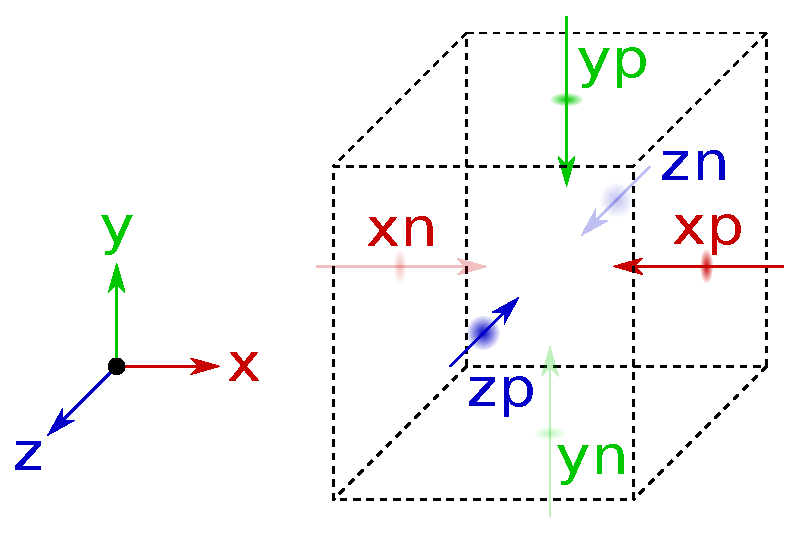
\includegraphics[width=0.4\linewidth]{3-Flow3DLabel}%
  \caption{Illustration of a region or subregion}%
  \label{fig:Flow3DLabel}
\end{figure}

In the implementation (\autoref{chap:Implementation}), subregions may be connected in multiple directions to form a \emph{\n{region}}.  A region is also a rectangular cuboid.  \autoref{fig:ModelHierarchy} shows the region and subregion within the model hierarchy.  However, this chapter only deals with one or two subregions at once.  Therefore, what will be called a subregion in the model implementation is often simply called a region in this chapter.

The subregion is the lowest level of spatial resolution, but it may contain multiple \emph{\n{species}} in multiple \emph{\np{phase}}.  Each of these \emph{\np{configuration}}, or species in certain phases, are treated as distinct but interacting entities.  The species and phases are also control volumes, but the model does not directly resolve the shape, location, and orientation of their boundaries.

Material, momentum, or energy may be \emph{transferred}\glsadd{transfer} among control volumes.  \emph{\N{material}} is synonymous with matter; it represents particles, atoms, or molecules.  Material is distinct from momentum and energy, although the transfer of material generally carries momentum and energy.  Since the model deals with chemical reactions and phase change, material is measured in terms of a number (which may be expressed in a unit such as the mole) rather than mass.  \N{material-adj} is also used as an adjective, as in material transfer.  \emph{\N{current}} is the flow rate of material, which may or may not be charged.  Electrical current is the flow rate of charge.  These and other key terms are listed in the glossary on page \pageref{mark:Glossary}.

There are two types of transfer.  \emph{Exchange} is transfer among different configurations within a subregion.  \emph{Transport} is transfer between similar configurations in neighboring subregions.  Thus, exchange is local and transport is spatial in nature.\footnote{Microscopically, exchange is also spatial, but the model is macroscopic.}  Chemical reactions and phases change involve material exchange---that is, transfer of matter among various configurations governed by the laws of chemistry.  Both types of transfer (exchange and transport) can generally occur by advection or diffusion.  These processes were introduced in \autoref{sec:DeclarativeLimitations} and will be discussed further in this chapter.

So far, two assumptions have been introduced: \begin{inparaenum}[(1)]\item all of the boundaries are rectangular and \item the subregions and regions have fixed boundaries\end{inparaenum}.  Further assumptions are introduced as necessary throughout the chapter.


It is important to note that the model equations are presented for a unit system where the gas and Faraday constants are normalized to one (see \autoref{sec:Units}).  This simplifies the equations and their implementation.  Also note that the \emph{\n{specific}} adjective is used to indicate ``per unit amount of material''.\footnote{In contrast, massic is defined by the \n{ISO} to mean ``per mass''~\cite{Taylor1995}.}  For example, specific mass is the mass per unit number of particles.  It is used instead of molar mass because the unit system is neutral with respect to the unit that represents the amount of material.  %A variable that represents the amount of material may be displayed in moles but the variable itself is not in moles (or any other unit of material).

\autoref{fig:AspectsOfFCModel} shows the high-level aspects that must be considered in a fuel cell model.  These will each be discussed in the following sections, with the exception of geometry (see above).  Many of the sections begin with a list of key features of the model that are either unusual or are new contributions.  The boxed equations are the ones that are actually implemented in the model (next chapter).  Other equations are presented to provide insight into the implemented equations and relate the model to established theories.

\begin{figure}[hbtp]
  \newcommand{\vgap}{\vphantom{Thermodynamic}}
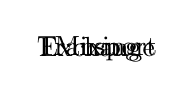
\begin{tikzpicture}
    [level distance=1.75cm]
    \Tree[.FC\\Model
           [.{Material\\Properties}
             [.{Thermodynamic\vgap} ]
%                [.{Correlated\vgap} ]
%                [.{Derived\vgap} ] ]
             [.{Diffusion\vgap} ] ] 
           [.{Geometry\vgap} ]
           [.{Processes\vgap}
             [.\node[xshift=-0.98mm]{Exchange\vgap}; ]
             [.\node[xshift=-0.98mm]{Transport\vgap}; ]
             [.\node[xshift=-0.98mm]{Mixing\vgap}; ] ]
           [.{Conservation\vgap} ] ]
  \end{tikzpicture}
  \caption{Considerations of a fuel cell model}
  \label{fig:AspectsOfFCModel}
\end{figure}


\section{Correlated Thermodynamic Properties}
\label{sec:CorrelatedThermo}

\begin{contextbox}
  Highlights:
  \begin{itemize*}
    \item The correlations are necessary and sufficient to calculate basic thermodynamic properties (specific entropy, enthalpy, Gibbs energy, etc.) given temperature and pressure or specific volume.
    \item The correlations are polynomial and can be expanded as needed for accuracy.
    \item The pressure-volume-temperature correlation is sufficiently general to describe ideal gases, real gases, and incompressible species with or without thermal expansion.  Many fuel cell models are explicitly based on ideal gases under incompressible flow~\cite{Bernardi1991, Ceraolo2003, Karnik2007, Kim2010, Natarajan2001, Nguyen1993, Rubio2010, Sivertsen2005, Spiegel2008, Springer1991, Sunden2011, Um2000, Um2004, Wang2001, Wang2006, Weber2004, Yuan2010}.
    % Less pertinent:~\cite{Chen2004, Mangold2010, Pukrushpan2002, Serincan2011}
    \item The specific heat capacity-temperature correlation is general enough to model media with constant specific heat or to provide accurate information on the temperature dependence.  This makes it possible to simplify the descriptions of inert gases (e.g., \s{N2}) and more accurately describe reacting gases (\s{H2}, \s{H2O}, and \s{O2}) to model the temperature dependence of the cell potential.
  \end{itemize*}
\end{contextbox}
\vspace{0.7\baselineskip}


\subsection{Isobaric Specific Heat Capacity-Temperature Relation}

Isobaric specific heat capacity is defined by
\begin{equation}
  \label{eq:cpDefinition}
  \s{c}[_p] \equiv \s{T}\diffp{\s{s}}{\s{T}}[_p]
\end{equation}
where \s{s}~is specific entropy, \s{T}~is temperature, and \s{p}~is pressure.  McBride et al.\ provide the isobaric specific heat capacity of many species as a correlated polynomial of temperature~\cite{McBride2002}; however, \s{c}[_p]~is in general a function of both temperature and pressure.  For condensed species, they specify the thermodynamic state by the actual temperature and a reference pressure (\SI{1}{atm}).  The state of gases is chosen to be the ideal gas at the given temperature, since the specific heat capacity of an ideal gas is independent of pressure.  The correlation for this adjusted isobaric specific heat capacity is
\begin{equation}
  \label{eq:cpo}
  \s{c}[_p][^o] = \s{b}_1\s{T}^{-2} + \s{b}_2\s{T}^{-1} + \s{b}_3 + \s{b}_4\s{T} + \s{b}_5\s{T}^2 + \s{b}_6\s{T}^3 + \s{b}_7\s{T}^4
  \glsadd{_123}
\end{equation}
The coefficients ($\s{b}_1$, $\s{b}_2\glsadd{_123}$, \dots) must be chosen for the proper temperature range but are otherwise constant.  The model uses a more general form
\begin{equation}
  \boxed{\s{c}[_p][^o] = \sum_{\s{i} = 1}^{\s{m}}\s{b}[_i]\s{T}^{\s{i} + \s{n} - 1}}
\end{equation}
where \s{n}~is the power of the first term and the polynomial has an arbitrary number of terms~(\s{m}).  The order of the polynomial is $\s{m} + \s{n} - 1$.  Multiple sets of coefficients may be specified; they are selected depending on the temperature range (as per McBride et al.).


\subsection{Pressure-Volume-Temperature Relation}

The model uses the virial \n{EOS}, which was proposed by Thiesen in 1885 and validated against many gases by Kammerling-Onnes in 1901~\cite{Morrison1985, Nag2008}. %, \cite[p.~336]{Nag2008}.
It is convenient for use with differential equations and can be expanded as needed for accuracy.  The virial \n{EOS} can be expressed in a volume-explicit (or Leiden~\cite{McGlashan1973}) form as
\begin{equation}
  \label{eq:VirialLeiden1}%
  \s{v} = \s{b}_1\group{\frac{\s{p}}{\s{T}}}^{-1} + \s{b}_2 + \s{b}_3\group{\frac{\s{p}}{\s{T}}}^{1} + \s{b}_4\group{\frac{\s{p}}{\s{T}}}^{2} + \ldots
  \glsadd{_123}
\end{equation}
where the coefficients are functions of temperature only\cite{Dymond2002}. %[Eq.\ 1.3]
The model uses the following generalized form
\begin{equation}
  \label{eq:VirialLeiden}
  \boxed{\s{v} = \sum_{i = 1}^{\s{m}_1}\,\sum_{j = 1}^{\s{m}_2}\s{b}\sub{_i}[_j]\group{\frac{\s{p}}{\s{T}}}^{\s{i} + \s{n}_1 - 1}\s{T}^{\s{j} + \s{n}_2 - 1}}
  \glsadd{_123}
  \glsadd{_abc}
\end{equation}
where $\s{n}_1$ and $\s{n}_2$ are the powers of the first term and the polynomial has an arbitrary numbers of terms in both dimensions ($\s{m}_1$, $\s{m}_2$).  The $\s{p}/\s{T}$ group is used instead of~\s{p} so that \begin{inparaenum}[(1)]\item the matrix of coefficients ($\s{b}\sub{_i}[_j]$) is more compact for typical correlations (e.g.,~\cite{Dymond2002}) and \item the virial inverse matrix ($\s{b}\sub{_i}[_j]\sup{^prime}$ below) has the same size\end{inparaenum}.

The virial coefficients may be derived from the statistical mechanics of intermolecular forces~\cite{Salzman2004}.  For gases, the first virial coefficient ($\s{b}_1\glsadd{_123}$) is generally the gas constant, which has been normalized to one.  The second virial coefficient characterizes binary interactions between molecules---specifically the pair energy potential function~\cite{Dymond2002}.  The third coefficient is for ternary interactions, the fourth is for quaternary interactions, and so on~\cite{McGlashan1973}.  These effects diminish rapidly with the order of the interaction~\cite{Present1958}.  If $\s{b}_1 = 1\glsadd{_123}$ and the other terms are neglected, the virial \n{EOS} reduces to the ideal gas \n{EOS}.  For gases at low pressures, only the first and possibly the second virial coefficients are necessary.  Dymond et al.\ correlate the second virial coefficients of many gases to polynomials in temperature~\cite{Dymond2002}.

\autoref{eq:VirialLeiden1} is suitable for incompressible or even constant-volume species, where only the second virial coefficient ($\s{b}_2\glsadd{_123}$) is nonzero.  If the species is compressible, the volume-explicit form of \autoref{eq:VirialLeiden1} is equivalent to the following pressure-explicit (or Berlin) form~\cite{McGlashan1973, Dymond2002}:%\cite[Eq.\ 1.2]{Dymond2002}
\begin{equation}
  \label{eq:VirialBerlin1}%
  \frac{\s{p}}{\s{T}} = \s{b}_1^\prime\s{v}^{-1} + \s{b}_2^\prime\s{v}^{-2} + \s{b}_3^\prime\s{v}^{-3} + \s{b}_4^\prime\s{v}^{-4} + \ldots
  \glsadd{^prime}\glsadd{_123}
\end{equation}
Otherwise, pressure cannot be determined from temperature and specific volume.  The model uses the following generalized form:
\begin{equation}
  \label{eq:VirialBerlin}
  \boxed{\s{v} = \sum_{i = 1 - \s{m}_1}^{0}\,\sum_{j = 1}^{\s{m}_2}\s{b}\sub{_i}[_j]\sup{^prime}\s{p}^{\s{i} + \s{n}_1}\s{T}^{\s{j} + \s{n}_2}}
  \glsadd{_123}
  \glsadd{_abc}
\end{equation}
The modified coefficients of \autoref{eq:VirialBerlin1} are directly related to those of \autoref{eq:VirialLeiden1}~\cite{McGlashan1973, Dymond2002}:%\cite[Eqs.\ 1.4--1.6]{Dymond2002}
\begin{subequations}%
  \begin{empheq}[box=\fbox]{align}
    \s{b}_1^\prime &= \s{b}_1\\
    \s{b}_2^\prime &= \s{b}_2\\
    \s{b}_3^\prime &= \s{b}_2^2 + \s{b}_3\\
    \s{b}_4^\prime &= \s{b}_2^3 + 3\s{b}_2\s{b}_3 + \s{b}_4%\\
%                   &= \s{b}_2\group{\s{b}_2^2 + 3\s{b}_3} + \s{b}_4\tag*{}
%     \s{b}_5^\prime &= \s{b}_2^4 + 6\s{b}_2^2\s{b}_3 + 2\s{b}_3^2 + 4\s{b}_2\s{b}_4 + \s{b}_5\\
%                   &= \s{b}_2\group{\s{b}_2\group{\s{b}_2^2 + 6\s{b}_3} + 4\s{b}_4} + 2\s{b}_3^2 + \s{b}_5\tag*{}%
    \glsadd{^prime}\glsadd{_123}
  \end{empheq}
\end{subequations}%
We can determine the relations for even higher-order coefficients by setting Equations~\ref{eq:VirialLeiden1} and \ref{eq:VirialBerlin1} equal (in terms of $\s{p}\s{v}/\s{T}$) and successively eliminating terms~\cite{Salzman2004}.

% ``Virial coefficients Bi appear as coefficients in the virial expansion of the pressure of a many-particle system in powers of the density, providing systematic corrections to the ideal gas law.  They are characteristic of the interaction potential between the particles and in general depend on the temperature.  The second virial coefficient [Background.tex] depends only on the pair interaction between the particles, the third [Background.tex] depends on 2- and non-additive 3-body interactions, and so on.'' [Wikipedia]

% ``Unlike empirical equations of state, such as the van der Waals equation (which is, at best, very approximate) and the Beattie-Bridgeman equation (which is now rarely used) which are discussed in GNS, the virial equation can be derived from exact statistical mechanical theory.'' [\url{http://voh.chem.ucla.edu/vohtar/spring06/classes/114/pdf/T9-Joule-Thomson%20Coefficient}]
% Originally from one of the following?
%   H. Kamerlingh Onnes (1901)
%   J. O. Hirschfelder, C. F. Curtiss, and R. B. Bird, Molecular Theory of Gases and Liquids, Wiley, New York, (1954)
%   W. J. Moore, Physical Chemistry, 4th ed., Prentice-Hall, Englewood Cliffs, N.J. (1972), pp.26, 130, 926.

% Also:  \cite[p. 379]{Brown2000}


\section{Derived Thermodynamic Properties}
\label{sec:DerivedThermo}

\begin{contextbox}
  Highlights:
  \begin{itemize*}
    \item The derivations are exact and do not involve additional assumptions besides those inherent in the correlated properties of \autoref{sec:CorrelatedThermo}.
    \item The properties are general and complete enough that the model does not require specialized thermodynamic correlations such as the saturation pressure-temperature curve of \n{H2O}.
  \end{itemize*}
\end{contextbox}
\vspace{0.7\baselineskip}

% \cite[pp.~16--18]{Dymond2002} provides equations for adjustment of properties from ideal gas, but they may be incorrect.


\subsection{Specific Entropy}
  \label{sec:SpecificEntropy}

We can write specific entropy as
\begin{equation}
  \s{s} = \int_0^{\s{T}}\frac{\s{c}[_p][^o]}{\s{T}}\,\mathrm{d}\s{T} + \int_{\s{p}[^o]}^{\s{p}}\diffp{\s{s}}{\s{p}}[_T]\mathrm{d}\s{p}%
\end{equation}
where $\s{c}[_p][^o]$ is evaluated at reference pressure $\s{p}[^o]$.  Applying the appropriate Maxwell relation, $(\partial\s{s}/\partial\s{p})_T = -(\partial\s{v}/\partial\s{T})_p$, this is
\begin{equation}
  \label{eq:s}
  \boxed{\s{s} = \int_0^{\s{T}}\frac{\s{c}[_p][^o]}{\s{T}}\,\mathrm{d}\s{T} - \int_{\s{p}[^o]}^{\s{p}}\diffp{\s{v}}{\s{T}}[_p]\mathrm{d}\s{p}}%
\end{equation}
which can be evaluated using Equations~\ref{eq:cpo} and \ref{eq:VirialLeiden1}.  McBride et al.~\cite{McBride2002} give the integration constant of the first term for each species so that the isobaric specific heat correlation does not need to be evaluated at (or even valid at) absolute zero temperature.  The second integral is $\ln{(\s{p}/\s{p}[^o])}$ for an ideal gas and typically small for condensed species.  Again, the second- and higher-order virial coefficients ($\s{b}_2$, $\s{b}_3\glsadd{_123}$, \dots) are functions of temperature but not pressure.  The coefficients of isobaric specific heat capacity ($\s{b}_1$, $\s{b}_2\glsadd{_123}$, \dots) may be treated as constant but must be chosen based on the temperature range.

For gases, the lower limit of the second integral of \autoref{eq:s} is evaluated only for the first virial coefficient.  This adjustment is necessary because the reference for the \s{c}[_p]-\s{T} correlation is the ideal gas instead of the real gas.  Formally, the modified form of \autoref{eq:s} for gases is
\begin{equation}
  \label{eq:sGas}
  \s{s} = \int_0^{\s{T}}\frac{\s{c}[_p][^o]}{\s{T}}\,\mathrm{d}\s{T} - \Group{\int_{\s{p}[^o]}^0\diffp{\s{v}[_IG]}{\s{T}}[_p]\mathrm{d}\s{p} + \int_0^{\s{p}}\diffp{\s{v}}{\s{T}}[_p]\mathrm{d}\s{p}}%
\end{equation}
where the first integral in square brackets involves the specific volume of the ideal gas and the second involves the real gas.  Following the approach by Rao~\cite{Rao1997}, %[p.~271]
the ideal gas contribution is integrated from the reference pressure to zero pressure and the real gas contribution is integrated from zero pressure to the actual pressure.  At zero pressure, binary and higher-order molecular interactions are eliminated and a real gas behaves as an ideal gas.

\autoref{fig:IntegrationPath} depicts the integration path of the pressure terms.  Assuming that the first virial coefficient ($\s{b}_1\glsadd{_123}$) is the same for the ideal gas and the real gas (since for gases $\s{b}_1 = 1\glsadd{_123}$), the contribution of the first-order virial term may be integrated directly from \s{p}[^o] to~\s{p}.  In effect, this combines $\ln{(0/\s{p}[^o])} + \ln{(\s{p}/0)}$ to give $\ln{(\s{p}/\s{p}[^o])}$.  Since the contributions of the second- and higher-order virial coefficients are zero at zero pressure, we can eliminate those integral evaluations.  The net result is that the lower limit of the second integral in \autoref{eq:s} is evaluated for the ideal gas and the upper limit is evaluated for the real gas.

\begin{figure}[htbp]
  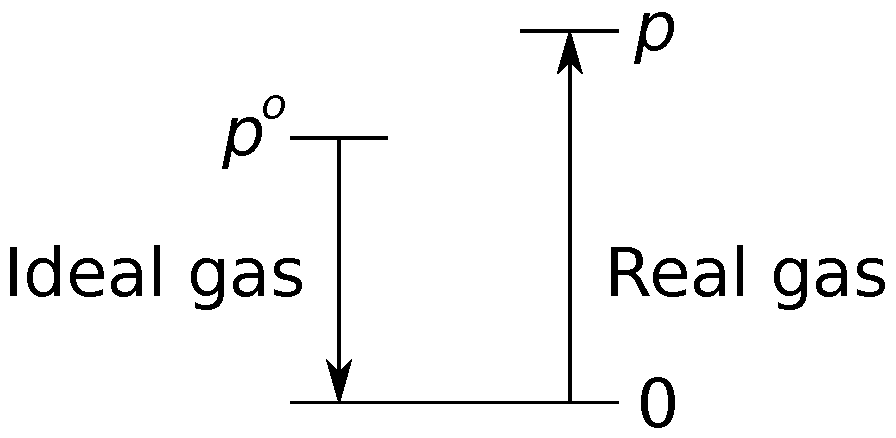
\includegraphics[width=0.3\linewidth]{3-IntegrationPath}%
  \caption{Integration path for the specific entropy of gases}%
  \label{fig:IntegrationPath}
\end{figure}

\subsection{Specific Enthalpy}

We can define specific enthalpy by the differential equation
\begin{equation}
  \label{eq:dh}%
  \mathrm{d}\s{h} = \s{T}\mathrm{d}\s{s} + \s{v}\mathrm{d}\s{p}
\end{equation}
After substituting \autoref{eq:s} and integrating with an adjustable temperature reference, this is
\begin{equation}
  \label{eq:h}%
  \boxed{\s{h} = \int_{\s{T}[^o]}^{\s{T}}\s{c}[_p][^o]\,\mathrm{d}\s{T} + \int_{\s{p}[^o]}^{\s{p}}\Group{\s{v} - \s{T}\diffp{\s{v}}{\s{T}}[_p]}\mathrm{d}\s{p}}%
\end{equation}
which can be evaluated using Equations~\ref{eq:cpo} and \ref{eq:VirialLeiden1}.  As for specific entropy, if the species is a gas, the lower limit of the second integral is of the ideal gas and the upper limit is of the real gas.  The second integral is zero for an ideal gas and typically small for condensed species.  McBride et al.~\cite{McBride2002} give the sufficient integration constants and offsets to specify the enthalpy reference such that \begin{inparaenum}[(1)]
  \item the enthalpy at \SI{0}{K} and \s{p}[^o]~is zero,
  \item the enthalpy at \SI{25}{\celsius} and \s{p}[^o]~is zero, or
  \item the enthalpy at \SI{25}{\celsius} and \s{p}[^o]~is the enthalpy of formation at that temperature and pressure.
\end{inparaenum}


\subsection{Specific Gibbs Energy}

We can define specific Gibbs energy by the following differential equation:
\begin{equation}
  \label{eq:GibbsFunction}
  \mathrm{d}\s{g} = \s{v}\mathrm{d}\s{p} - \s{s}\mathrm{d}\s{T}
\end{equation}
In conjunction with \autoref{eq:dh}, this implies that
\begin{equation}
  \label{eq:g}
  \s{g} = \s{h} - \s{T}\s{s}
\end{equation}
Substituting Equations~\ref{eq:s} and \ref{eq:h},
\begin{equation}
  \label{eq:gExpanded}
  \boxed{\s{g} = \int_{\s{p}[^o]}^{\s{p}}\s{v}\,\mathrm{d}\s{p} + \s{T}\int_{\s{p}[^o]}^{\s{p}}\diffp{\s{v}}{\s{T}}[_p]\mathrm{d}\s{p} - \int_{\s{p}[^o]}^{\s{p}}\s{T}\diffp{\s{v}}{\s{T}}[_p]\mathrm{d}\s{p} + \int_{\s{T}[^o]}^{\s{T}}\s{c}[_p][^o]\,\mathrm{d}\s{T} - \s{T}\int_0^{\s{T}}\frac{\s{c}[_p][^o]}{\s{T}}\,\mathrm{d}\s{T}}%
\end{equation}
which can be evaluated using Equations~\ref{eq:cpo}, \ref{eq:VirialLeiden1}, and \ref{eq:VirialBerlin1}.  If the species is a gas, the lower limits of the pressure integrals are of the ideal gas and the upper limits are of the real gas (see \autoref{sec:SpecificEntropy}).

% Electrochemical free potential of species is the sum of Gibbs potential and electric work potential \cite[Equation~3.16, p.~82]{Newman1991}:
% \begin{equation}
%   \s{mu}[_i] = \s{mu}[_i]^{chem} + \s{z}[_i]\s{Phi}
% \end{equation}
% Electrical work potential is the work required to bring the particles together from infinite distance slowly (i.e., electrostatic) [\url{http://en.wikipedia.org/wiki/Electric_potential_energy}].

% Discussion of conflicting names for chemical and electrochemical potential: \url{http://www.tf.uni-kiel.de/matwis/amat/def_en/kap_2/advanced/t2_4_1.html}


\subsection{Isobaric Specific Heat Capacity}

We can express the isobaric specific heat capacity by substituting \autoref{eq:s} into \autoref{eq:cpDefinition}.
\begin{equation}
  \label{eq:cp}
  \boxed{\s{c}[_p] = \s{c}[_p][^o] - \s{T}\diffp{\Group{\int_{\s{p}[^o]}^{\s{p}}\diffp{\s{v}}{\s{T}}[_p]\mathrm{d}\s{p}}}{\s{T}}[_p]}%
\end{equation}
This can also be evaluated using Equations~\ref{eq:cpo} and \ref{eq:VirialLeiden1}.  The second term is zero for an ideal gas and usually small for condensed species.  If the species is a gas, the lower limit of the integral is of the ideal gas and the upper limit is of the real gas (see \autoref{sec:SpecificEntropy}).


\subsection{Isochoric Specific Heat Capacity}

Isochoric specific heat capacity is defined by
\begin{equation}
  \label{eq:cvDefinition}
  \s{c}[_v] \equiv \s{T}\diffp{\s{s}}{\s{T}}[_v]
\end{equation}
The isochoric and isobaric specific heat capacities are related by the following equation~\cite{Moran2004}: %[p.~546]
\begin{equation}
  \boxed{\s{c}[_v] = \s{c}[_p] - \s{T}\diffp{\s{p}}{\s{T}}[_v]\diffp{\s{v}}{\s{T}}[_p]}
\end{equation}
Applying \autoref{eq:cp}, this is
\begin{equation}
  \s{c}[_v] = \s{c}[_p][^o]- \s{T}\Group{\diffp{\s{p}}{\s{T}}[_v]\diffp{\s{v}}{\s{T}}[_p] + \diffp{\Group{\int_{\s{p}[^o]}^{\s{p}}\diffp{\s{v}}{\s{T}}[_p]\mathrm{d}\s{p}}}{\s{T}}[_p]}%
\end{equation}
which can be evaluated using Equations~\ref{eq:cpo}, \ref{eq:VirialLeiden1}, and \ref{eq:VirialBerlin1}.  It reduces to $\s{c}[_v] = \s{c}[_p] - 1$ for an ideal gas.  If the species is a gas, the lower limit of the integral is of the ideal gas and the upper limit is of the real gas (see \autoref{sec:SpecificEntropy}).


\section{Mixtures}
\label{sec:Mixtures}

\begin{contextbox}
  Highlights:
  \begin{itemize*}
    \item Traditionally, Dalton's and Amagat's laws are used with the ideal gas assumption, but the model does not impose that requirement.\footnote{This is an approximation.  The alternative would to formulate another, more detailed p-v-T relation that encompasses the entire mixture---possibly as a correction pressure or volume.  That is beyond the present scope.}
    \item The volumes and pressures of mixtures can change dynamically, but the model imposes Dalton's and Amagat's laws exactly and instantaneously.  %For example, the volumes of the phases always add to the total volume of the region.
    There are no additional states.
  \end{itemize*}
\end{contextbox}
\vspace{0.7\baselineskip}

% \begin{figure}[!htb]
%   \newcommand{\vgap}{\vphantom{Mixing}}
%   \centering
%   \begin{tikzpicture}
%     [level distance=1.5cm,
%      level 2/.style={level distance=1.1cm}]
%     \Tree[.FC\\Model
%            [.{Processes\vgap}
%               [.{Mixing\vgap}
%                 [.{Additivity\\of Pressure} ]
%                 [.{Additivity\\of Volume} ] ] ] ]
%   \end{tikzpicture}
%   \caption{Types of mixing regimes in the fuel cell model}
% \end{figure}

% Departures from Dalton's and Amagat's laws:~\cite{Din1965}

% \cite{Woo1995}:
% ``The significance of the preceding derivation is that, in a mixture of gases (black and white), Dalton's law calculates the properties of a gas (black) assuming the other gas (white) is not there, whereas Amagat's law calculates the properties of the black molecules assuming that the white molecules are there and interact with the black just as do other black molecules.  Put another way, the ideal gas law assumes that molecules are blind, they `see' no other molecules; Dalton's law assumes that the molecules are selectively blind, they see only molecules of their own `color'; Amagat's law assumes that the molecules are colorblind, they `see' all molecules but think they are the same color.''

% Gibbs-Dalton law is an extension of Dalton's law of additive pressures applied to an ideal gas \url{http://www.scribd.com/doc/27396916/187/Gibbs-Dalton-law}.

% Amagat's law is analogous to the serial connection of many particles (pressures equal at a point, length is additive) and Dalton's law is analogous to the parallel connection of many particles (each species is a branch; lengths equal, pressures additive).


\subsection{Species within a Phase}
\label{sec:DaltonsLaw}

The model combines species within a phase using Dalton's law of partial pressures, which states that the partial pressures of the components of a mixture add to the total pressure of the mixture~\cite{Bejan2006}:%[p.~192]
\begin{equation}
  \boxed{\s{p} = \sum\s{p}[_i]}
\end{equation}
Dalton's law also states that each species~\s{i} exists at the total volume of the phase:
\begin{equation}
  \boxed{\s{V}[_i] = \s{V}}
\end{equation}
For example, according to this concept, the atmospheric gases of~\s{N2}, \s{O2}, etc.\ each occupy the total volume of the air but only contribute partially to the pressure of the air.


\subsection{Phases within a Region}
\label{sec:AmagatsLaw}

The model combines phases within a region using Amagat's law of partial volumes, which states that the partial extensive volumes of the components of a mixture sum to the total extensive volume of the mixture~\cite{Bejan2006}:%[p.~194]
\begin{equation}
  \boxed{\s{V} = \sum\s{V}[_i]}
\end{equation}
In the model, \s{V}[_i]~is the volume of a phase and \s{V}~is the volume of the region, which is fixed.  Amagat's law also states that each species~\s{i} exists at the total pressure of the phase:
\begin{equation}
  \boxed{\s{p}[_i] = \s{p}}
\end{equation}

The model only uses Amagat's law for distinct phases within a region---not for species within a phase.  Amagat's law loses its physical meaning as species are mixed~\cite{Woo1995}.  If species are fully mixed, it is impossible to distinguish the particles and thus determine the partial volumes.

For example, if a system contains a solid phase and air, the model states that the solid and the air experience the same pressure and occupy only part of the total volume (Amagat's law).  Within the air, the gases mix according to Dalton's law (\autoref{sec:DaltonsLaw}).  The model applies Dalton's law and Amagat's law dynamically, which makes it possible to describe the formation of liquid water in the cell~\cite{Bevers1997, Li2005, Weber2004ChemRev}.

The model is classified as a Euler-Euler approach rather than a Euler-Lagrange approach~\cite{Fluent6.3}, since all phases are tracked from a Eulerian perspective.  The volume fractions are continuous functions of time and must sum to one.  The Euler-Lagrange approach is limited to problems where the solid phase has a small volume in comparison to the fluid phase---10\% to 12\%~\cite{Fluent6.3}.  This is not appropriate for the layers of a fuel cell.


\section{Basic Conservation Equations}
\label{sec:BasicConservation}

\begin{contextbox}
  Highlights:
  \begin{itemize*}
    \item The model is dynamic.  It includes material, momentum, and energy storage.
    \item Each species has its own conservation equations for material, translational momentum, and energy.  However, the model's parameters can be set so that the translation tool combines certain conservation equations through index reduction.  The concept of separate momentum balances for each species is unusual but not unprecedented in the literature~\cite{Wesselingh2000, Kerkhof2005AIChE, Kerkhof2005ChemEngSci}.  Separate energy balances are rarely used (\cite{Kuropatenko2005} is one example).
  \end{itemize*}
\end{contextbox}
\vspace{0.7\baselineskip}

Material, momentum, and energy are conserved throughout the model at interfaces and within regions.  Each configuration (i.e., each species in each phase) has its own conservation equation in every region.  The conserved quantities can be stored in configurations but not at interfaces between or among configurations.

Below, the conservation equations (i.e., balances) are introduced with minimal detail to explain the exchange and transport equations (Sections~\ref{sec:Exchange} and \ref{sec:Transport}).  The interfaces are generalized here, but there are two types:  boundaries between regions (for transport) and transitions among configurations within a region (for exchange).  In general, the flow through each interface has advective and diffusive components.  Later, in \autoref{sec:DetailedConservation}, detailed conservation equations will be presented.


\subsection{Material}
\label{sec:BasicMaterialBalance}


The rate of storage of material is equal to the net rate of intake or transfer of material into a control volume.  \autoref{fig:MaterialIntake} shows that there are two types of material transfer---exchange and transport.  In general, exchange and transport can each occur by advection or diffusion.  However, the model considers chemical reactions and phase change, the two modes of material exchange, to be diffusive processes.

\begin{figure}[hbtp]
  \newcommand{\vgap}{\vphantom{Body}}
  \begin{tikzpicture}
    [level distance=1.75cm]
    \Tree[.{Material\\transfer}
           [.{Transport\vgap}
             [.{Advective\vgap} ]
             [.{Diffusive\vgap} ] ]
           [.{Exchange\vgap}
             [.{Diffusive\vgap}
               [.{Chemical\\(reaction)\vgap} ]
               [.{Physical\\(phase change)\vgap} ] ] ] ]
  \end{tikzpicture}
  \caption{Types of material intake considered in the model}
  \label{fig:MaterialIntake}
\end{figure}


For now, the material balance will be written simply as
\begin{equation}
  \newcommand{\vgap}{\vphantom{\diffp{\s{N}}{\s{t}}}}
  \label{eq:MaterialBalance}%
  \boxed{\underbrace{\vgap\diffp{\s{N}}{\s{t}}}_\text{storage} =  \,\, \underbrace{\vgap\sum\dot{N}[_i]}_\text{intake}}
\end{equation}
where \s{N}~is the particle number or amount of material and \dot{N}[_i] is the total current (advective and diffusive, $\dot{N}\sub{_A}[_i] + \dot{N}\sub{_D}[_i]$) into a generalized interface~\s{i}.  The use of a partial derivative ($\diffp{\s{N}}{\s{t}}$) rather than a total derivative ($\frac{\mathrm{d}\s{N}}{\mathrm{d}\s{t}}$) serves as a reminder that the model is Eulerian.  Although the equation is written in terms of material, mass is conserved as well since the specific mass of each configuration is constant and the phase change and reaction processes are balanced in terms of mass.

At boundaries and transitions, there is no material storage.  Advection has no net effect because the rate of advection is continuous across a boundary.  Therefore, the material balance reduces to
\begin{equation}
  \label{eq:MaterialBalanceInterface}
  \boxed{0 = \sum\dot{N}\sub{_D}[_i]}
\end{equation}
where the summation is now across all interacting configurations~\s{i}.  This equation is generated automatically by the connection equations of the \n{EOO} language; it is the generalized Kirchhoff current law for material.


\subsection{Rotational Momentum}
\label{sec:RotationalConservation}

The model is based on the assumption that rotational momentum is not stored.  Rotational momentum is not exchanged or transported axially through boundaries, but it is conveyed through shear forces.  We assume that the forces are point forces in the center of the boundaries and that the axes of rotation are centered in the region.  Therefore,
\begin{subequations}
  \label{eq:RotationalConservation}
  \begin{empheq}[box=\fbox]{align}
    0 &= \group{\dot{mPhi}\sub{_z}[_neg][_y] - \dot{mPhi}\sub{_z}[_pos][_y]}\s{L}[_z] - \group{\dot{mPhi}\sub{_y}[_neg][_z] - \dot{mPhi}\sub{_y}[_pos][_z]}\s{L}[_y] \label{eq:RotationalConservationX} \\
    0 &= \group{\dot{mPhi}\sub{_x}[_neg][_z] - \dot{mPhi}\sub{_x}[_pos][_z]}\s{L}[_x] - \group{\dot{mPhi}\sub{_z}[_neg][_x] - \dot{mPhi}\sub{_z}[_pos][_x]}\s{L}[_z] \label{eq:RotationalConservationY} \\
    0 &= \group{\dot{mPhi}\sub{_y}[_neg][_x] - \dot{mPhi}\sub{_y}[_pos][_x]}\s{L}[_y] - \group{\dot{mPhi}\sub{_x}[_neg][_y] - \dot{mPhi}\sub{_x}[_pos][_y]}\s{L}[_x] \label{eq:RotationalConservationZ}
  \end{empheq}
\end{subequations}
where $\dot{mPhi}\sub{_z}[_neg][_y]$ is the force in the y-direction through the negative-z boundary, $\dot{mPhi}\sub{_y}[_pos][_z]$ is the force in the z direction through the positive-y boundary, and so on.  The normal forces do not introduce torque since they are aligned with the center of rotation.  These equations are included in the diffusion equations for shear force around each axis (\autoref{sec:TransverseTransport}).


\subsection{Translational Momentum}
\label{sec:BasicTranslationalBalance}


The rate of storage of translational momentum is equal to the sum of the forces on a control volume.  As shown by \autoref{fig:MaterialIntake}, there are three types of forces on a configuration within a region: body forces, surface forces, and intermolecular forces.  The body forces may be gravitational or electric; magnetic and nuclear forces are assumed to be negligible.  The surface forces include the effects of thermodynamic pressure, advection (i.e., dynamic pressure), and diffusion (i.e., nonequilibrium pressure~\cite{Meier2005} and shear stress).  The thermodynamic pressure is always normal to the surface, but advection and diffusion also have transverse components.  The intermolecular or exchange forces may be advective or diffusive.  Advective exchange occurs, for example, in a reacting stream where the reactants are traveling relative to the control volume.  Diffusive exchange occurs in multi-component fluids when the species are traveling at different velocities.

\begin{figure}[hbtp]
  \newcommand{\vgap}{\vphantom{Body}}
  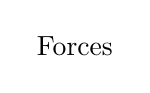
\begin{tikzpicture}
    [level distance=1.75cm]
    \Tree[.\node[xshift=-0.3mm]{Forces\vgap};
           [.{Body\vgap}
             [.{Gravi-\\tational} ]
             [.{Electric\vgap} ] ]
           [.{Transport\\(surface)}
             [.{Pressure\vgap}
               [.{Thermo-\\dynamic} ]
               [.{Advective\\(dynamic)}
                 [.{Normal\vgap} ]
                 [.{Transverse\vgap} ] ] ]
             [.{Diffusive\\(viscous)}
                 [.{Normal\\(bulk)\vgap} ]
                 [.{Transverse\\(shear)} ] ] ]
           [.{Exchange\\(intermolecular)}
             [.{Advective\vgap} ]
             [.{Diffusive\vgap} ] ] ]
  \end{tikzpicture}
  \caption{Types of forces considered in the model}
  \label{fig:Forces}
\end{figure}


For now, we will generalize the advective and diffusive forces to encompass both exchange and transport.  We will also combine the normal and transverse components of transport.  Therefore, the translational momentum balance can be written as
\begin{equation}
  \newcommand{\vgap}{\vphantom{\diffp{\group{\s{M}\s{phi}}}{\s{t}}}}%
  \label{eq:TranslationalBalance}%
  \underbrace{\diffp{\group{\s{M}\s{phi}}}{\s{t}}}_\text{storage} + \underbrace{\vgap\s{M}\s{a} + \s{Z}\s{E}}_\text{body} + \underbrace{\vgap\s{A}\Delta\s{p}[_i]}_{\substack{\text{thermo-}\\\text{dynamic}}} = \sum\Big(\underbrace{\vgap\s{m}\s{phi}[_i]\dot{N}[_i]}_\text{advection} + \underbrace{\vgap\dot{mPhi}\sub{_D}[_i]}_\text{diffusion}\Big)
\end{equation}
where \s{phi}~is a component of velocity, \s{E}~is the electric field, and \s{a}~represents the acceleration due to additional body forces.  The mass \s{M}~is $\s{m}\s{N}$ and the charge \s{Z}~is $\s{z}\n{N}$, where \s{m}~is the specific mass, \s{z}~is the charge number, and \s{N}~is the amount of material known from the state of the material balance~(\ref{eq:MaterialBalance}).  The diffusive terms (\dot{mPhi}[_D]) include shear forces, nonequilibrium normal forces, and drag among configurations.

The advective forces ($\s{m}\s{phi}\dot{N}$) account for convective acceleration and the momentum transferred in reacting flows and phase change.  It is important to note again that the material transfer (\dot{N}) includes both advection and diffusion.  Momentum is advected or carried by material regardless of whether that material is transferred by advection or diffusion.

The difference ($\Delta$) on the left side of \autoref{eq:TranslationalBalance} is across the boundaries normal to the component of translational momentum.  The variable~\s{A} is the area of those boundaries.  The thermodynamic force term ($\s{A}\Delta\s{p}[_i]$) is based on the assumption that the configuration experiences pressure across the entire cross-sectional area of the region, although in reality the area is reduced if other phases are present.  This is necessary to ensure that translational momentum is conserved between two adjacent regions.


At boundaries and transitions, there is no storage.  The advective terms of \autoref{eq:TranslationalBalance} cancel because the advected properties are continuous at the interface.  The thermodynamic pressure is continuous at the interface and thus has no effect.  There is no material in the interface, so there are no body forces.  Therefore, the conservation of translational momentum reduces to
\begin{equation}
  \label{eq:TranslationalBalanceInterface}
  \boxed{0 = \sum\dot{mPhi}\sub{_D}[_i]}
\end{equation}
where the summation is now across all interacting configurations~\s{i}.  This equation is generated automatically by the connection equations of the \n{EOO} language; it is the generalized Kirchhoff current law for translational momentum.


\subsection{Energy}
\label{sec:BasicEnergyBalance}


The rate of storage of energy in a control volume is equal to the net rate of intake.  As shown in \autoref{fig:EnergyIntake}, the intake can be divided into material, translational, and thermal parts.  Although not shown, each of these forms may be transferred by exchange or transport.  The translational and thermal energy transfers can be due to advection or diffusion.  The material transfer of energy is not labeled as advective or diffusive in \autoref{fig:EnergyIntake} because it requires further explanation.  The material itself can be transferred by advection or diffusion, but the associated energy transfer is purely advective because the energy is carried by material.

\begin{figure}[hbtp]
  \newcommand{\vgap}{\vphantom{($\frac{1}{2}\s{m}\s{phi}^2$)}}
  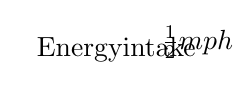
\begin{tikzpicture}
    [level distance=1.75cm]
    \Tree[.\node[xshift=-5.7mm]{Energy\\intake};
            [.{Material\\(\s{g})\vgap} ]
            [.{Translational\vgap}
              [.{Advective\\($\frac{1}{2}\s{m}\s{phi}^2$)\vgap} ]
              [.{Diffusive\\(viscous)\vgap} ] ]
            [.{Thermal\vgap}
              [.{Advective\\(\s{T}\s{s})\vgap} ]
              [.{Diffusive\\(conduction)\vgap} ] ] ]
  \end{tikzpicture}
  \caption{Types of energy intake considered in the model}
  \label{fig:EnergyIntake}
\end{figure}

Thermal conduction is synonymous with thermal diffusion.  Thermal convection is the combined effect of diffusive thermal exchange between phases (often a solid and a fluid) and the subsequent transport of thermal energy via advection of the fluid.  The thermal advection factor ($\s{T}\s{s}$) and the material factor~(\s{g}) constitute specific enthalpy ($\s{h} = \s{g} + \s{T}\s{s}$, \autoref{eq:g}).  Combined with the translational advection factor, this is specific enthalpy plus specific kinetic energy ($\s{h} + \frac{1}{2}\s{m}\s{phi}^2$).


The factors of \autoref{fig:EnergyIntake} are incorporated into the right side of the energy balance equation:
\begin{equation}
  \newcommand{\vgap}{\vphantom{\frac{\s{m}\s{phi}[_i]^2}{2}\dot{N}[_i] + \s{phi}[_i]\dot{mPhi}\sub{_D}[_i]}}
  \label{eq:EnergyBalance}
  \underbrace{\underbrace{\vgap\s{g}\diffp{\s{N}}{\s{t}}}_\text{material} \, + \underbrace{\vgap\frac{\partial\group{\s{M}\s{phi}^2}}{2\partial\s{t}}}_\text{translational} + \,\, \underbrace{\vgap\s{T}\diffp{\s{S}}{\s{t}}}_\text{thermal}}_\text{storage} \,\, = \,\, \underbrace{\sum\Big[\underbrace{\vgap\s{g}[_i]\dot{N}[_i]}_\text{material} + \underbrace{\s{phi}[_i]\Big(\underbrace{\vgap\frac{\s{m}\s{phi}[_i]}{2}\dot{N}[_i]}_\text{advection} + \underbrace{\vgap\dot{mPhi}\sub{_D}[_i]}_\text{diffusion}\Big)}_\text{translational} + \underbrace{\vgap\underbrace{\vgap\group{\s{T}\s{s}}[_i]\dot{N}[_i]}_\text{advection} + \underbrace{\vgap\dot{Q}\sub{_D}[_i]}_\text{diffusion}}_\text{thermal}\Big]}_\text{intake}
\end{equation}
where \dot{N}[_i] is the total current (advective and diffusive) into interface~\s{i}.  This equation applies to every species in every phase.  It has been assumed that the control volume is stationary with respect to external fields (e.g., no gravitational work), although the fluid may move against those fields within the control volume.   The translational diffusion term, in conjunction with the translational (or kinetic) storage term, accounts for viscous dissipation.  This will be more apparent in later forms of the energy balance (e.g.,~\autoref{eq:EnergyBalanceIntensive2}).

The material and thermal storage terms ($\s{g}\diffp{\s{N}}{\s{t}} + \s{T}\diffp{\s{S}}{\s{t}}$) are equivalent to $\diffp{\s{H}}{\s{t}} - \s{V}\diffp{\s{p}}{\s{t}}$ or $\diffp{\s{U}}{\s{t}} + \s{p}\diffp{\s{V}}{\s{t}}$, where $\s{p}\diffp{\s{V}}{\s{t}}$ is the boundary work done by the configuration.\footnote{The form of \autoref{eq:EnergyBalance} has been chosen so that the material, translational, and thermal terms are explicit on both sides.  Specific flow work (\s{p}\s{v}) is considered a part of the material term.}  The boundary work can only be due to expansion of the phases in which the configuration belongs (and contraction of other phases) because the volume of the region is fixed.  The translational storage term describes the change in macroscopic kinetic energy.


At boundaries and transitions, there is no energy storage.  The advective terms cancel because the advected properties are continuous at the interface.  The translational diffusion terms can be removed because they sum to zero according to \autoref{eq:TranslationalBalanceInterface}.  Therefore, the conservation of energy reduces to
\begin{equation}
  \label{eq:ThermalBalanceInterface}
  \boxed{0 = \sum\dot{Q}\sub{_D}[_i]}
\end{equation}

where the summation is now across all interacting configurations~\s{i}.  This equation is generated automatically by the connection equations of the \n{EOO} language; it is the generalized Kirchhoff current law for heat transfer.


\section{Exchange Equations}
\label{sec:Exchange}

\begin{contextbox}%
  Highlights:
  \begin{itemize*}
    \item A common modeling framework is used for phase change, intermolecular drag, and intermolecular thermal conduction.
    \item The transfer of translational momentum and energy due to phase change and reactions is described as pure advection.
    \item An analogy is established between the total (advective plus diffusive) rate of exchange and the material derivative.
    \item The model describes phase change dynamically.  It does not assume instantaneous phase equilibrium in the sense of the Gibbs phase rule~\cite{Moran2004, Bejan2006}.  This avoids nonlinear systems of equations while using the previously established properties (i.e., no need to establish a separate correlation for saturation pressure).
    \item The rate of phase change is proportional to the difference in chemical activity between the phases.
    \item A property called independity is defined which generalizes the concept of mobility for translational interactions to thermal interactions.
  \end{itemize*}
\end{contextbox}

% \begin{figure}[!htb]
%   \newcommand{\vgap}{\vphantom{Exchange}}
%   \centering
%   \begin{tikzpicture}
%     [level distance=1.5cm,
%      level 2/.style={level distance=1.1cm}]
%     \Tree[.FC\\Model
%            [.{Processes\vgap}
%               [.{Exchange\vgap}
%                 [.{Advection\vgap} ]
%                 [.{Diffusion\vgap} ] ] ] ]
%   \end{tikzpicture}
%   \caption{Types of exchange processes in the fuel cell model}
% \end{figure}

\emph{\N{exchange}} is the transfer of a conserved quantity---material, momentum, or energy---among different configurations of material that exist within a region.  In general, it is due to advection and diffusion.  Advective exchange is the transfer of the quantity along with a sustained transfer of material between species (i.e., reaction) or different phases of a single species (i.e., phase change).  Diffusive exchange is the transfer of the quantity due only to collisions or thermal agitation of the particles, without a sustained material transfer.  In diffusion, a particle leaves one configuration (i.e., a species in a certain phase) with the specific quantity (or particle-average amount of the quantity) within the configuration and returns with the specific quantity of the other configuration.  This brings certain intensive properties---specific Gibbs energy, velocity, and temperature---into equilibrium among the configurations.


The model of exchange is based on the assumption that advection and diffusion are independent yet additive.  The total rate of exchange of the quantity~\s{X} into a configuration~\s{j} due to interaction or transition~\s{i} is the sum of the advective and diffusive rates:
\begin{equation}
  \label{eq:Exchange}
  \dot{X}\sub{_i}[_j] = \dot{X}\sub{_A}[ ][_i][_j] + \dot{X}\sub{_D}[ ][_i][_j]
\end{equation}
For material exchange, the quantity~(\s{X}) is the amount of material~(\s{N}).   For translational exchange, it is the product of the amount of material and velocity~(\s{Phi}).  For thermal exchange, it is heat~(\s{Q}).  The phase change and reaction processes are purely advective in terms of translational momentum and energy.  Particles from the source (e.g., reactants) carry properties through the process without intermediately mixing with particles from the sink (e.g., products).  Meanwhile, there are diffusive interactions for translational momentum and energy that are independent of the phase change and reactions.



\noindent\underline{\textbf{Advection}}

The rate of advective exchange is the product of the current and the amount of the exchanged quantity carried by the material.
\begin{equation}
  \label{eq:AdvectiveExchange1}
  \dot{X}\sub{_A}[ ][_i][_j] = \dot{N}\sub{_i}[_j]\diffp{\s{X}}{\s{N}}[_i][_j]
\end{equation}
The variable $\dot{N}\sub{_i}[_j]$ is the rate of material exchange.  Both $\dot{N}\sub{_i}[_j]$ and $\dot{X}\sub{_A}[ ][_i][_j]$ are due to the interaction~(\s{i}) and are directed into the configuration~(\s{j}).


The partial derivative, $\partial\s{X}/\s{N}$, is an intensive property.  For material advection, it is unity (1);\footnote{\label{fn:NoAdvectiveMaterialExchange}In this case \autoref{eq:AdvectiveExchange1} reduces to an identity and is removed from the model.  This is consistent with the previous statement (\autoref{sec:BasicMaterialBalance}) that the only mode of material exchange is diffusion.} for translational exchange, it is velocity~(\s{phi}); and for thermal exchange, it is the product of specific entropy and temperature ($\s{s}\s{T}$).  Since advection and diffusion are independent, there is no intermediate mixing between the sources and sinks.  Therefore, the upwind scheme is appropriate.  Here, it is applied locally among configurations rather than spatially between regions.  Using the upwind scheme, the previous equation (\ref{eq:AdvectiveExchange1}) can be written as
\begin{equation}
  \label{eq:AdvectiveExchange2}
  \dot{X}\sub{_A}[ ][_i][_j] = \dot{N}\sub{_i}[_j]\cdot
  \begin{cases}%
    \diffp{\s{X}}{\s{N}}[_j] & \text{if $\dot{N}\sub{_i}[_j] < 0$ (source),} \\
    \diffp{\s{X}}{\s{N}}[_i] & \text{if $\dot{N}\sub{_i}[_j] > 0$ (sink)}
  \end{cases}
\end{equation}
The factor $\diffp{\s{X}}{\s{N}}[_i]$ is called the \emph{\n{conversion property}} because it is the property at which the sources (e.g., reactants) are converted to the sinks (e.g., products).  The designations of source and sink depend on the direction of the phase change or reaction at a given time.



\noindent\underline{\textbf{Diffusion}}

We can consider the rate of diffusive exchange to be the material derivative or the rate of transfer experienced by the particles themselves.\footnote{See the discussion on \pageref{mark:TransportDiscussion}.}
\begin{equation}
  \label{eq:DiffusiveExchange1}
  \dot{X}\sub{_D}[ ][_i][_j] = \Diff{\s{X}}{\s{t}}[_i][_j]
\end{equation}
$(\mathrm{D}\s{t})\sub{_i}[_j]$ is the product of the mean collision interval (\s{tau}[_j]) between particles and $8/3\pi$ as a result of the Einstein relation.  We will assume that the exchanged quantity is linear with respect to an intensive driving property \s{gamma}; therefore, $(\mathrm{D}\timessep\s{X})\sub{_i}[_j] = (\s{gamma}[_i] - \s{gamma}[_j])(\partial\s{X}/\partial\s{gamma})\sub{_j}$.  The following assumptions have also been implied:
\begin{enumerate*}
  \item The collision events are frequent enough for the average collision interval to be meaningful.  This implies that the mean free path, or the average distance traveled between collisions, is much smaller than the length scale of the problem.  It is not the case for example in effusion~\cite{Present1958}.
  \item Between collisions the particles have no influence on one another.
  \item The properties of a particle depend only on those of the last particle with which it collided.
\end{enumerate*}
In practice, these assumptions may be relaxed by using empirical diffusion coefficients (see \autoref{sec:ExchangeProperties}).  It follows that

\begin{equation}
  \label{eq:DiffusiveExchange2}
  \frac{8}{3\pi}\s{tau}[_j]\timessep\dot{X}\sub{_D}[ ][_i][_j] = \s{k}\sub{_i}[_j]\diffp{\s{X}}{\s{gamma}}[_j]\group{\s{gamma}[_i] - \s{gamma}[_j]}
\end{equation}

where the dimensionless adjustment factor $\s{k}\sub{_i}[_j]$ has been introduced to account for the effect of geometry (e.g., one gas species will typically be coupled more strongly to another than to a solid species) and to add the degrees of freedom necessary to match an arbitrary set of Maxwell-Stefan binary diffusion coefficients (see \autoref{sec:MS}).  It is one by default.  If two or more interacting configurations have collision intervals of zero, their driving properties (\s{gamma}[_j]) will be equal.  The transported quantity will be exchanged without loss and the number of dynamic states will be reduced.  The partial derivative $\group{\partial\s{X}/\partial\s{gamma}}_j$ is an extensive property of the configuration.  For material exchange, it is volume; for translational exchange, it is amount of material; and for thermal exchange, it is heat capacity.  The variable~\s{gamma}[_i] is called the \emph{\n{mediation property}} because it is the property to which the differences among the interacting configurations are mediated at a given time (not necessarily the equilibrium or steady-state value).


\noindent\underline{\textbf{Discussion}}
\label{mark:TransportDiscussion}


The total rate of exchange (\autoref{eq:Exchange}) can be expanded with the rates of advection and diffusion from Equations \ref{eq:AdvectiveExchange1} and \ref{eq:DiffusiveExchange1}:
\begin{equation}
  \dot{X}\sub{_i}[_j] = \dot{N}\sub{_i}[_j]\diffp{\s{X}}{\s{N}}[_i][_j] + \Diff{\s{X}}{\s{t}}[_i][_j]
\end{equation}
Since the model uses a Eulerian perspective, the total exchange rate $\dot{X}\sub{_i}[_j]$ is actually a partial derivative in the form of $\partial\s{X}/\partial\s{t}$.  Dropping the subscripts and rearranging, the previous equation becomes\label{mark:MaterialDeriv}
\begin{equation}
  \Diff{\s{X}}{\s{t}} = \diffp{\s{X}}{\s{t}} - \dot{N}\diffp{\s{X}}{\s{N}}
\end{equation}
This is essentially the definition of a material derivative~\cite{Bird2007}, but in terms of current instead of velocity.  Usually, the scalar property in the material derivative is intensive---for example, the diffusion-driving property~(\s{gamma})---but it is coupled to the exchanged property~(\s{X}) through the extensive property $\partial\s{X}/\partial\s{gamma}$.  The usual advective term $\boldsymbol{\s{phi}}\cdot\boldsymbol{\nabla}\s{X}$ is a loss.  The advective source is $-\boldsymbol{\s{phi}}\cdot\boldsymbol{\nabla}\s{X}$ or $\dot{N}\partial\s{X}/\partial\s{N}$, although the material exchange current itself is purely diffusive (as mentioned previously).  The concept here is that particles experience the collisions that lead to diffusive exchange, but they do not experience advection.  Advection is an artifact of the Eulerian basis of the model.

There are several types of material exchange processes.  The simplest is phase change, which is discussed in the following section.  Electrochemical reactions are introduced later (\autoref{sec:Reaction}) because they involve geometric dimensions and orientation like the transport equations (also to follow).  Chemical reactions are beyond the present scope; they are only intermediate to the electrochemical reactions in a fuel cell.


\subsection{Phase Change}
\label{sec:PhaseChange}


At equilibrium, a species has the same specific Gibbs energy in each phase.  The configurations may equilibrate rapidly~\cite{Oh1996}, yet the model still considers the process to be dynamic.  This avoids the nonlinear system of equations that would occur since the Gibbs function (\autoref{eq:gExpanded}) is only invertible in certain cases.  In terms of Gibbs' phase rule\label{mark:Gibbs} ($\s{n}[_DOF] = 2 + \s{n}[_spec] - \s{n}[_phases]$)~\cite{Moran2004, Bejan2006}, %\cite[pp.~24--49]{Bejan2006}
we are not subtracting the number of phase equilibria ($\s{n}[_phases] - 1$).  Therefore, the number of thermodynamic state variables or degrees of freedom is one plus the number of species ($\s{n}[_DOF] = 1 + \s{n}[_spec]$).\footnote{In fact, without certain optional assumptions enabled (see \autoref{sec:Phases}) the model often has even more thermodynamic state variables.  The number of thermodynamic state variables in the model is the number of species plus the number of compressible species, and there are often several compressible species in a region.  In general, the total number of state variables is equal to the number of ways in which energy (not limited to thermal and compressive) may be stored.}

Since the phase change model is dynamic, it is necessary to specify the rate of phase change.  One way would be to assume that the rate is proportional to the difference between the vapor pressure and the saturation pressure.  Yet this would not avoid nonlinear equations because the saturation pressure is only implicitly known from the thermodynamic properties established in Sections~\ref{sec:CorrelatedThermo} and \ref{sec:DerivedThermo}.  We could implement a known correlation for saturation pressure (e.g.,~\cite{Springer1991} or~\cite{ModelicaSL3.2}), but this would be redundant and somewhat inconsistent with the existing properties.  Another way would be to assume that the rate of phase change is proportional to the differences in specific Gibbs energies between the phases.  However, this does not relate well to the classical Hertz-Knudsen equation~\cite{Ytrehus1997} which establishes the rate in proportion to the difference in adjusted concentrations.  Many other approaches could be used~\cite{Bedeaux2003}, but these are more detailed than presently necessary and more complicated than can be efficiently implemented.

The model uses a fairly simple approach that is based on the differences of chemical activities.  It is consistent with the generalized equation for diffusive exchange (\ref{eq:DiffusiveExchange2}) with some additional assumptions.  It results in linear systems of equations and avoids the need for conditional expressions and dynamic state selection.


\subsubsection{Context}

In a \n{PEMFC}, water may be absorbed and desorbed between the ionomer and the gas in the catalyst layer, as shown in \autoref{fig:PhaseChangeIonomer}.  The catalyst layer extends from the plane where the solid is entirely the \n{GDL} material to the plane where the solid is entirely the ionomer or proton exchange material.  \autoref{fig:PhaseChangeLiquid} shows that water may also condense and evaporate between the liquid and gas in the flow plate, the \n{GDL}, or the catalyst layer.  In any case, there is an interface between the phases.  The interface is only a volumeless threshold, but we will assume that there is a transition or surface layer on the condensed side.

\begin{figure}[htbp]
  \subfloat[Gas to ionomer]{
    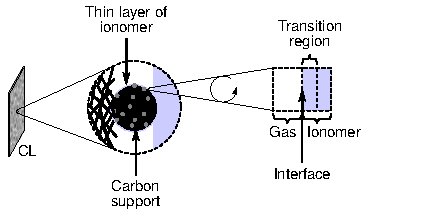
\includegraphics[width=0.65\linewidth]{3-PhaseChangeIonomer}%
    \label{fig:PhaseChangeIonomer}
  }\quad
  \subfloat[Gas to liquid]{
    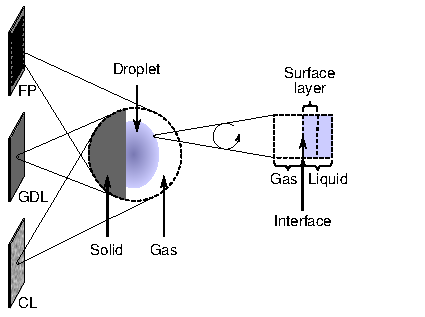
\includegraphics[width=0.65\linewidth]{3-PhaseChangeLiquid}%
    \label{fig:PhaseChangeLiquid}
  }
  \caption[Locations of the phase change processes]{Phase change occurs between the gas and \subref{fig:PhaseChangeIonomer} the ionomer in the catalyst layers (CLs) and \subref{fig:PhaseChangeLiquid} the liquid in the flow plates (FPs), gas diffusion layers (GDLs), and CLs}
  \label{fig:PhaseChangeContext}
  \glsadd{_l}\glsadd{_ionomer}
\end{figure}


\subsubsection{Equations}

The rate of condensation or absorption is given by the diffusive exchange equation (\ref{eq:DiffusiveExchange2}) for material ($\s{X} = \s{N}$, $\s{gamma} = \s{rho}$, $\partial\s{X}/\partial\s{gamma} = \s{V}$).\footnote{Phase change is purely diffusive.  As mentioned in \autoref{fn:NoAdvectiveMaterialExchange}, the advective exchange equation (\ref{eq:AdvectiveExchange1}) is not applicable to material exchange.}
\begin{equation}
  \label{eq:PhaseChange1a}
  \frac{8}{3\pi}\s{tau}[_c]\timessep\dot{N}\sub{_D}[ ][_i][_c] = \s{k}\sub{_i}[_c]\s{V}[_c]\group{\s{rho}[_i] - \s{rho}[_c]}
\end{equation}
where the subscript~c denotes the condensed or absorbed phase.  Since $\s{rho} = \s{N}/\s{V}$,
\begin{equation}
  \label{eq:PhaseChange2a}
  \frac{8}{3\pi}\s{tau}[_c]\timessep\dot{N}\sub{_D}[ ][_i][_c] = \s{k}\sub{_i}[_c]\s{N}[_c]\group{\frac{\s{rho}[_i]}{\s{rho}[_c]} - 1}
\end{equation}
We will assume that the species behaves as an isothermal ideal gas over the transition region or surface layer.  Under these conditions, \autoref{eq:GibbsFunction} evaluates to
\begin{equation}
  \s{g}[_i] - \s{g}[_c] = \s{T}[_c]\ln\group{\frac{\s{rho}[_i]}{\s{rho}[_c]}}
\end{equation}
Therefore, the rate of condensation or absorption can be written as
\begin{equation}
  \label{eq:PhaseChange}
  \boxed{\s{tau}\sub{_i}[_c]\sup{^prime}\timessep\dot{N}\sub{_D}[ ][_i][_c] = \s{N}[_c]\Group{\exp\group{\frac{\s{g}[_i] - \s{g}[_c]}{\s{T}[_c]}} - 1}}
\end{equation}
where \s{tau}[^prime]~is the effective collision interval, or the mean time between collisions that yield phase change:
\begin{equation}
  \label{eq:EffectiveCollisionInterval}
  \boxed{\s{tau}\sub{_i}[_c]\sup{^prime} = \frac{8}{3\pi\s{k}\sub{_i}[_c]}\s{tau}[_c]}
\end{equation}
In practice, $\s{tau}\sub{_i}[_c]\sup{^prime}$~is an empirical, tunable parameter.  Since we have assumed that the entire transition region is within the condensed phase, the gas is in equilibrium with the condition at the interface.
\begin{equation}
  \label{eq:PhaseChange3b}
  \boxed{\s{g}[_i] = \s{g}[_g]}
\end{equation}
where the subscript~\s{g} denotes the gas phase.  Therefore,
\begin{equation}
  \label{eq:PhaseChange4}
  \s{tau}\sub{_i}[_c]\sup{^prime}\timessep\dot{N}\sub{_D}[ ][_i][_c] = \s{N}[_c]\Group{\exp\group{\frac{\s{g}[_g] - \s{g}[_c]}{\s{T}[_c]}} - 1}
\end{equation}
This can also be written in terms of activity referenced to the condensed phase.
\begin{equation}
  \s{tau}\sub{_i}[_c]\sup{^prime}\timessep\dot{N}\sub{_D}[ ][_i][_c] = \s{N}[_c]\group{\s{a}[_g] - \s{a}[_c]}
\end{equation}
which is consistent with the common interpretation of activity as an effective, dimensionless concentration.


This model is appropriate for condensation and evaporation or absorption and desorption.  It should be noted that if the condensed phase is entirely absent ($\s{N}[_c] = 0$), there can be no condensation.  If phase change is included, the conditions are set so that some amount of material (as slight as it may be) always exists in the condensed or absorbed phase.

If the effective collision interval is zero ($\s{tau}\sub{_i}[_c]\sup{^prime} = 0$), then the phases will be in perfect equilibrium.  Then, it is no longer a dynamic process, and in general, there will be nonlinear systems of equations.  Since phase change is a diffusive process, the equilibration is irreversible.  Heat is generated in phase~\s{j} at the rate of $\dot{N}\sub{_D}[ ][_i][_j]\group{\s{g}[_i] - \s{g}[_j]}$ (discussed further in \autoref{sec:EnergyBalance}).  However,  this is zero for the gas phase due to \autoref{eq:PhaseChange3b}.  This excludes the latent heat, which is transferred via thermal advective exchange (\autoref{sec:ThermalAdvectiveExchange}).


\subsection{Drag and Translational Advection}
\label{sec:TranslationalExchange}

The translational exchange equations follow from the generalized exchange equations (\ref{eq:AdvectiveExchange2} and \ref{eq:DiffusiveExchange2}).  The exchanged quantity~(\s{X}) is the product of the amount of material and velocity~(\s{Phi}).  Both the intensive property $\partial\s{X}/\partial\s{N}$ %(or $\partial\s{Phi}/\partial\s{N}$)
and the diffusion-driving property~(\s{gamma}) are velocity~(\s{phi}).  The extensive property $\partial\s{X}/\partial\s{gamma}$ %(or $\partial\s{Phi}/\partial\s{phi}$)
is the amount of material~(\s{N}).


\subsubsection{Advection}


Advective translational exchange occurs in a stream of fluid that is undergoing phase change or reaction.  It is not significant in the reactions of a \n{PEMFC} since they occur at the surface of stationary electrodes.  However, the model includes advective translational exchange for completeness; it may be important in other devices.


In terms of translational exchange, \autoref{eq:AdvectiveExchange2} is the following:
\begin{equation}
  \label{eq:TranslationalAdvectiveExchange1}
  \dot{Phi}\sub{_A}[ ][_i][_j] = \dot{N}\sub{_i}[_j]\cdot
  \begin{cases}%
    \s{phi}[_j] & \text{if $\dot{N}\sub{_i}[_j] < 0$ (source),} \\
    \s{phi}[_i] & \text{if $\dot{N}\sub{_i}[_j] > 0$ (sink)}
  \end{cases}
\end{equation}
However, the product of the amount of material and velocity~(\s{Phi}) is not generally conserved.  Momentum, \s{mPhi}, is.  Therefore, we will multiply the previous equation by specific mass so that it can be written in terms of forces or rates of momentum:
\begin{equation}
  \label{eq:TranslationalAdvectiveExchange}
  \boxed{\dot{mPhi}\sub{_A}[ ][_i][_j] = \s{m}[_j]\dot{N}\sub{_i}[_j]\cdot
  \begin{cases}%
    \s{phi}[_j] & \text{if $\dot{N}\sub{_i}[_j] < 0$ (source),} \\
    \s{phi}[_i] & \text{if $\dot{N}\sub{_i}[_j] > 0$ (sink)}
  \end{cases}}
\end{equation}

The variable~\s{phi}[_i]~is the \emph{\n{conversion velocity}}, or the velocity at which the products are generated from the reactants during advective exchange.  Its value is a consequence of conservation at the interface (\autoref{eq:TranslationalBalanceInterface}).  Since advection and diffusion are independent, the sum of the advective forces ($\dot{mPhi}\sub{_A}[ ][_i][_j]$) over all of the interacting configurations is zero.  Using \autoref{eq:TranslationalAdvectiveExchange}, this is
\begin{equation}
  0 = \sum_{\s{j} \in \s{xi}[_i]}\s{m}[_j]\dot{N}\sub{_i}[_j]\cdot
  \begin{cases}%
    \s{phi}[_j] & \text{if $\dot{N}\sub{_i}[_j] < 0$ (source),} \\
    \s{phi}[_i] & \text{if $\dot{N}\sub{_i}[_j] > 0$ (sink)}
  \end{cases}
\end{equation}
where \s{xi}[_i]~is the set of the configurations that interact at transition~\s{i}.  The currents ($\dot{N}\sub{_i}[_j]$) are related by the stoichiometry of the phase change or reaction.
\begin{equation}
  \dot{N}\sub{_i}[_j] = \s{n}\sub{_i}[_j]\dot{N}[_i]
\end{equation}
where \dot{N}[_i]~is the rate of the transition~\s{i} and $\s{n}\sub{_i}[_j]$~is the stoichiometric coefficient of configuration~\s{j} with respect to transition~\s{i}.  Therefore,
\begin{equation}
  0 = \sum_{\s{j} \in \s{xi}[_i]}\s{m}\sub{_i}[_j]\s{n}\sub{_i}[_j]\cdot
  \begin{cases}%
    \s{phi}[_j] & \text{if $\s{n}\sub{_i}[_j]\dot{N}[_i] < 0$ (source),} \\
    \s{phi}[_i] & \text{if $\s{n}\sub{_i}[_j]\dot{N}[_i] > 0$ (sink)}
  \end{cases}
\end{equation}
Solving for the conversion velocity,
\begin{equation}
  \label{eq:ConversionVelocity1}
  \s{phi}[_i] = \frac{\sum_{\s{j}\in\text{source}}\left|\s{n}\sub{_i}[_j]\right|\s{m}[_j]\s{phi}[_j]}{\sum_{\s{j}\in\text{sink}}\left|\s{n}\sub{_i}[_j]\right|\s{m}[_j]}
\end{equation}
where the numerator is summed over the sourcing configurations (reactants) and the denominator is summed over the sinking configurations (products).  If the process is well-posed, it must conserve mass ($\sum_{\s{j}\in\text{source}}|\s{n}\sub{_i}[_j]|\s{m}[_j] = \sum_{\s{j}\in\text{sink}}|\s{n}\sub{_i}[_j]|\s{m}[_j]$), and
\begin{equation}
  \label{eq:ConversionVelocity2}
  \s{phi}[_i] = \frac{\sum_{\s{j}\in\text{source}}\left|\s{n}\sub{_i}[_j]\right|\s{m}[_j]\s{phi}[_j]}{\sum_{\s{j}\in\text{source}}\left|\s{n}\sub{_i}[_j]\right|\s{m}[_j]}
\end{equation}
Thus, the conversion velocity is the mass-weighted average of the velocities of the configurations consumed by the process.


\subsubsection{Diffusion}

For translational exchange, \autoref{eq:DiffusiveExchange2} is the following:
\begin{equation}
  \label{eq:TranslationalDiffusiveExchange1}
  \frac{8}{3\pi}\s{tau}[_j]\timessep\dot{Phi}\sub{_D}[ ][_i][_j] = \s{k}\sub{_i}[_j]\s{N}[_j]\group{\s{phi}[_i] - \s{phi}[_j]}
\end{equation}
This can be written as
\begin{equation}
  \label{eq:TranslationalDiffusiveExchange}
  \boxed{\s{mu}[_j]\timessep\dot{mPhi}\sub{_D}[ ][_i][_j] = \s{k}\sub{_i}[_j]\s{N}[_j]\group{\s{phi}[_i] - \s{phi}[_j]}}
\end{equation}
where \s{mu}[_j]~is the mobility:
\begin{equation}
  \label{eq:Mobility}
  \boxed{\s{mu} = \frac{8}{3\pi\s{m}}\s{tau}}
\end{equation}

The variable~\s{phi}[_i]~is the \emph{\n{mediation velocity}}.  Like the conversion velocity, it can be determined from conservation at the interface.  Since advection and diffusion are independent, the sum of the diffusion forces ($\dot{mPhi}\sub{_D}[ ][_i][_j]$) over all of the interacting configurations is zero.  Using \autoref{eq:TranslationalDiffusiveExchange}, this is
\begin{equation}
  0 = \sum_{\s{j} \in \s{xi}[_i]}\left.\group{\s{phi}[_i] - \s{phi}[_j]}\s{k}\sub{_i}[_j]\s{N}[_j]\middle/\s{mu}[_j]\right.
\end{equation}
where \s{xi}[_i]~is the set of all the interacting configurations at transition~\s{i}.  Solving for the mediation velocity,
\begin{equation}
  \label{eq:MediationVelocity}
  \s{phi}[_i] = \frac{\sum_{\s{j} \in \s{xi}[_i]}\left.\s{phi}[_j]\s{k}\sub{_i}[_j]\s{N}[_j]\middle/\s{mu}[_j]\right.}{\sum_{\s{j} \in \s{xi}[_i]}\left.\s{k}\sub{_i}[_j]\s{N}[_j]\middle/\s{mu}[_j]\right.}
\end{equation}
This indicates that the mediation velocity is a conductance-weighted average of the velocities of the interacting configurations.  The previous equation applies to each set~\s{xi} associated with each interaction~\s{i}.  Each set can have a different value of the mediation velocity.


\subsection{Thermal Conduction and Advection}
\label{sec:ThermalExchange}

The translational exchange equations follow from the generalized exchange equations (\ref{eq:AdvectiveExchange2} and \ref{eq:DiffusiveExchange2}).  The exchanged quantity~(\s{X}) is heat~(\s{Q}).  The intensive property $\partial\s{X}/\partial\s{N}$ is the product of specific entropy and temperature ($\partial\s{Q}/\partial\s{N} = \s{T}\partial\s{S}/\partial\s{N} = \s{T}\s{s}$).  The diffusion-driving property~(\s{gamma}) is temperature~(\s{T}).  The extensive property $\partial\s{X}/\partial{\s{gamma}}$ is heat capacity~(\s{C}).  The heat capacity is isobaric (\s{C}[_p]), since the pressures of the configurations are assumed to be at equilibrium (see \autoref{sec:AmagatsLaw}).


\subsubsection{Advection}
\label{sec:ThermalAdvectiveExchange}

In terms of thermal exchange, \autoref{eq:AdvectiveExchange2} is
\begin{equation}
  \label{eq:ThermalAdvectiveExchange}
  \boxed{\dot{Q}\sub{_A}[ ][_i][_j] = \dot{N}\sub{_i}[_j]\cdot
  \begin{cases}%
    \group{\s{s}\s{T}}\sub{_j} & \text{if $\dot{N}\sub{_i}[_j] < 0$ (source),} \\
    \group{\s{s}\s{T}}\sub{_i} & \text{if $\dot{N}\sub{_i}[_j] > 0$ (sink)}
  \end{cases}}
\end{equation}

where \s{j}~is a configuration that participates in reaction or phase change~\s{i}.  It is important to note that \dot{Q}[_A] is advective.  It is different from \dot{Q}[_D], which is the rate of thermal diffusion or conduction.  In the energy balance (\autoref{eq:EnergyBalance}), the $\s{s}\s{T}$ factor combines with the specific Gibbs energy~(\s{g}) to give the specific enthalpy~(\s{h}) that is transferred with the process (reaction or phase change).  The rate of thermal energy due to $\sum\dot{N}[_j]\group{\s{s}\s{T}}[_j]$ or $\dot{N}\sum\s{n}[_j]\group{\s{s}\s{T}}[_j]$ over a process (where the subscript~\s{i} has been dropped) is split stoichiometrically (not by mass) among the products (sinks).  The intensive properties of the reactants (sources) are not directly affected due to the conditional factor in \autoref{eq:ThermalAdvectiveExchange}.  If the process occurs near equilibrium, then $\sum\s{n}[_j]\s{g}[_j]$ is nearly zero and $\sum\s{n}[_j]\group{\s{s}\s{T}}[_j]$ is nearly $\sum\s{n}[_j]\s{h}[_j]$, the enthalpy of the reaction or phase change.  If the process is not at equilibrium, heat is produced at the rate of $\dot{N}\sum\s{n}[_j]\s{g}[_j]$.  This is irreversible because the process always occurs towards lower specific Gibbs energy.\footnote{This was evident from the equation for the rate of phase change (\ref{eq:PhaseChange}) and is also the case in electrochemical reactions, inclusive of the electrical work potential (\autoref{sec:Reaction}).}

The property $\group{\s{s}\s{T}}[_i]$~is the thermal conversion property---the product of specific entropy and temperature at which the products are generated from the reactants during advective exchange.  Its value is a consequence of conservation at the interface (\autoref{eq:ThermalBalanceInterface}).  Since advection and diffusion are independent, the sum of the advective rates ($\dot{Q}\sub{_A}[ ][_i][_j]$) over all of the interacting configurations is zero.  Using \autoref{eq:ThermalAdvectiveExchange}, this is
\begin{equation}
  0 = \sum_{\s{j} \in \s{xi}[_i]}\dot{N}\sub{_i}[_j]\cdot
  \begin{cases}%
    \group{\s{s}\s{T}}[_j] & \text{if $\dot{N}\sub{_i}[_j] < 0$ (source),} \\
    \group{\s{s}\s{T}}[_i] & \text{if $\dot{N}\sub{_i}[_j] > 0$ (sink)}
  \end{cases}
\end{equation}
where \s{xi}[_i]~is the set of the configurations that interact at transition~\s{i}.  The currents ($\dot{N}\sub{_i}[_j]$) are related by the stoichiometry of the phase change or reaction.
\begin{equation}
  \dot{N}\sub{_i}[_j] = \s{n}\sub{_i}[_j]\dot{N}[_i]
\end{equation}
where $\dot{N}[_i]$ is the rate of the transition~\s{i} and $\s{n}\sub{_i}[_j]$~is the stoichiometric coefficient of configuration~\s{j} with respect to transition~\s{i}.  Therefore,
\begin{equation}
  0 = \sum_{\s{j} \in \s{xi}[_i]}\s{n}\sub{_i}[_j]\cdot
  \begin{cases}%
    \group{\s{s}\s{T}}[_j] & \text{if $\s{n}\sub{_i}[_j]\dot{N}[_i] < 0$ (source),} \\
    \group{\s{s}\s{T}}[_i] & \text{if $\s{n}\sub{_i}[_j]\dot{N}[_i] > 0$ (sink)}
  \end{cases}
\end{equation}
Solving for the thermal conversion property,
\begin{equation}
  \label{eq:ThermalConversionProperty}
  \group{\s{s}\s{T}}[_i] = \frac{\sum_{\s{j}\in\text{source}}\left|\s{n}\sub{_i}[_j]\right|\group{\s{s}\s{T}}[_j]}{\sum_{\s{j}\in\text{sink}}\left|\s{n}\sub{_i}[_j]\right|}
\end{equation}
where the numerator is summed over the sourcing configurations (reactants) and the denominator is summed over the sinking configurations (products).  Thus, the thermal conversion property is the stoichiometrically-weighted average of the specific entropy-temperature products (or specific enthalpy-specific Gibbs energy differences) of the configurations consumed by the process.



\subsubsection{Diffusion}

For thermal diffusion (i.e., thermal conduction), \autoref{eq:DiffusiveExchange2} is
\begin{equation}
  \label{eq:ThermalDiffusiveExchange1}
  \frac{8}{3\pi}\s{tau}[_j]\timessep\dot{Q}\sub{_D}[ ][_i][_j] = \s{k}\sub{_i}[_j]\s{C}\sub{_p}[_j]\group{\s{T}[_i] - \s{T}[_j]}
\end{equation}
This can be written as
\begin{equation}
  \label{eq:ThermalDiffusiveExchange}
  \boxed{\s{nu}[_j]\timessep\dot{Q}\sub{_D}[ ][_i][_j] = \s{k}\sub{_i}[_j]\s{N}[_j]\group{\s{T}[_i] - \s{T}[_j]}}
\end{equation}
where \s{nu}[_j]~is called thermal \emph{\n{independity}} here.\footnote{This is the thermal analog of mobility, but there is no established name.  It is not called resistivity.  Resistivity is resistance times the quotient of area and length, whereas independity is resistance (or \emph{\n{independence}}) times the amount of material.}  It is defined by
\begin{equation}
  \label{eq:ThermalIndependity}
  \boxed{\s{nu} = \frac{8}{3\pi\s{c}[_p]}\s{tau}}
\end{equation}

The variable~\s{T}[_i]~is the \emph{\n{mediation temperature}}.  Like the thermal conversion property, it can be determined from conservation at the interface.  Since advection and diffusion are independent, the sum of the heat flow rates ($\dot{Q}\sub{_D}[ ][_i][_j]$) over all of the interacting configurations is zero.  Therefore, the sum of \autoref{eq:ThermalDiffusiveExchange} is
\begin{equation}
  0 = \sum_{\s{j} \in \s{xi}[_i]}\left.\group{\s{T}[_i] - \s{T}[_j]}\s{k}\sub{_i}[_j]\s{N}[_j]\middle/\s{nu}[_j]\right.
\end{equation}
where \s{xi}[_i]~is the set of all the interacting configurations at transition~\s{i}.  Solving for the mediation temperature,
\begin{equation}
  \label{eq:MediationProperty}
  \s{T}[_i] = \frac{\sum_{\s{j} \in \s{xi}[_i]}\left.\s{T}[_j]\s{k}\sub{_i}[_j]\s{N}[_j]\middle/\s{nu}[_j]\right.}{\sum_{\s{j} \in \s{xi}[_i]}\left.\s{k}\sub{_i}[_j]\s{N}[_j]\middle/\s{nu}[_j]\right.}
\end{equation}
This indicates that the mediation temperature is a conductance-weighted average of the temperatures of the configurations interacting by diffusion.  The previous equation applies to each set~\s{xi} associated with each interaction~\s{i}.  Each set can have a different value of the mediation temperature.


\section{Exchange Properties}
\label{sec:ExchangeProperties}

The base factor in the diffusive exchange properties is the collision interval or the mean time between collisions.  It depends on the thermodynamic state and possibly other properties, but it can be estimated from kinetic theory under the following assumptions~\cite{Present1958}:
\begin{enumerate*}
  \item The particles are smooth and rigid but elastic spheres with identical radii.  This is the ``billiard-ball'' assumption.  It implies that the collisions are instantaneous and conserve kinetic energy.
  \item The mean free path, or the average distance a particle travels between collisions, is much larger than the diameter of a particle.
  \item The speeds of the particles follow the Maxwell-Boltzmann distribution.
\end{enumerate*}

With these assumptions, the mean free path is
\begin{equation}
  \label{eq:MeanFreePath}
  \boxed{\s{lambda} = \frac{\s{v}}{\sqrt{2}\pi\s{d}^2\s{q}}}
\end{equation}
where \s{v}~is the specific volume of the particles (reciprocal of concentration), \s{d}~is the specific rigid-sphere or Van der Waals diameter, and \s{q}~is the particle number representing a single particle~\cite{Present1958, Cercignani1962}. %\cite[pp.~31--32]{Present1958}, \cite[p.~229]{Cercignani1962}
The denominator is the product of the intercept area per particle with particles of the same type ($\pi\s{d}^2\s{q}$) and a correction due to the Maxwell-Boltzmann distribution ($\sqrt{2}$).\footnote{It is counterintuitive that the distribution of molecular speeds has an effect on the mean free path, but this has been established in the literature \cite[p.~32]{Present1958}.}  The derivation is beyond the present scope (see \cite[pp.~31--32]{Present1958} and \cite[p.~229]{Cercignani1962}).  The collision interval is the mean free path divided by the mean thermal speed ($\sqrt{8\s{T}/\pi\s{m}}$):
\begin{equation}
  \label{eq:CollisionInterval}
  \boxed{\s{tau} = \s{lambda}\sqrt{\frac{\pi\s{m}}{8\s{T}}}}
\end{equation}
The collision interval is called the relaxation time in solid state physics~\cite{Ashcroft1976}.  For a typical species, the collision interval is small.  For oxygen as an ideal gas at \SI{25}{\celsius} and 21\% of atmospheric pressure, the specific volume~(\s{v}) is \SI{0.12}{m^3/mol}.  The diameter of a particle is approximately \SI{220}{pm}; therefore the mean free path is approximately \SI{0.9}{\micro\metre} and the collision interval is approximately \SI{2}{ns}.

The effective collision interval, which is used for phase change, can be determined from the collision interval using \autoref{eq:EffectiveCollisionInterval}.  Mobility and thermal independity can be determined from the collision interval using Equations \ref{eq:Mobility} and \ref{eq:ThermalIndependity}.  Due to the assumptions implicit in the diffusive exchange equation (\ref{eq:DiffusiveExchange2}), the equations for the effective collision interval, mobility, and thermal independity are only taken to be estimates.  However, they are useful if more precise data is not available.


\section{Transport Equations}
\label{sec:Transport}

% **current is linear, not velocity.

\begin{contextbox}
  Highlights:
  \begin{itemize*}
    \item The model describes the transport of every species individually, even in purely advective flow.  However, the diffusive exchange of translational momentum (\autoref{sec:Reaction}) tends to couple the velocities of the species and thus the rates of advective transport.
    \item A general transport equation is proposed to handle upstream discretization.  It meets the exact solution to a mixed advection\slash{}diffusion problem~\cite{Patankar1980}.
    \item The transport equation changes continuously from neutral discretization under pure diffusion to complete upstream discretization in the limiting case of pure advection.  This avoids switching events that could slow the simulation if diffusion were not included.
    \item The model is expressed in resistivity instead of conductivity so that it is well-posed under all representable values.
    \item The model allows zero or finite dynamic compressibility.  The reciprocal, bulk viscosity, is rarely studied~\cite{Rah1999} and seldom included in fluid simulations~\cite{Meier2005}, let alone fuel cell simulations.  The associated effect may be neglected for monoatomic ideal gases and incompressible fluids~\cite{Kerkhof2005ChemEngSci, Meier2005}, but following a plausible formation (see \autoref{sec:MaterialTransport}) the effect is dominant for lightweight particles such as electrons.
    \item The material transport equation combines the effects of self diffusivity and bulk viscosity to describe material advection and diffusion.  That way, the same equations can describe the primarily advective flow down the channels of a \n{PEMFC} and the primarily diffusive flow through the layers.
  \end{itemize*}
\end{contextbox}

% \begin{figure}[!htb]
%   \newcommand{\vgap}{\vphantom{Transport}}
%   \centering
%   \begin{tikzpicture}
%     [level distance=1.5cm,
%      level 2/.style={level distance=1.1cm}]
%     \Tree[.FC\\Model
%            [.{Processes\vgap}
%               [.{Transport\vgap}
%                 [.{Advection\vgap} ]
%                 [.{Diffusion\vgap} ] ] ] ]
%   \end{tikzpicture}
%   \caption{Types of transport processes in the fuel cell model}
% \end{figure}

\emph{\N{transport}} is the transfer of a conserved quantity between adjacent regions.  Like exchange (\autoref{sec:Exchange}), it is due to advection and diffusion.  Advective transport is the transfer of the quantity along with a sustained transfer of material between regions.  Diffusive transport is the transfer of the quantity due only to collisions or thermal agitation of the particles, without a sustained material transfer.  In diffusion, a particle leaves one region with the specific quantity (or particle-average amount of the quantity) within the configuration and returns with the specific quantity of the other configuration.  This brings certain intensive properties---concentration, velocity, and temperature---into equilibrium among the configurations.  Since these properties are sufficient to set the thermodynamic state, other properties (e.g., pressure) equilibrate as well.

In transport, unlike exchange, advection and diffusion are not independent.  The transport equations are based on the following assumptions:
\begin{enumerate*}

  \item Transport of material, momentum, and energy only occurs between like configurations (e.g., liquid water).  Bulk transport is only the net, macroscopic effect of individual species flows.  The inter-configurational effects (e.g., between liquid water and water vapor) are described within a region via exchange (\autoref{sec:Exchange}).

  \item \label{itm:AssumeAligned} The coordinate system is aligned with the principle axes of transport.  For example, if a phase is stratified within a region, the layers must be parallel to one of the planes in the rectilinear grid.  This implies that a gradient which induces diffusion along an axis does not induce diffusion along axes orthogonal to it~\cite{Bejan2006}.%[pp.~691--692].
  \item There is no radiative heat transfer.
\end{enumerate*}

The total rate of transport of a quantity~\s{X} into configuration~\s{j} from boundary~\s{i} is the sum of the advective and diffusive rates:
\begin{equation}
  \label{eq:Transport}
  \dot{X}[_i] = \dot{X}\sub{_A}[ ][_i] + \dot{X}\sub{_D}[ ][_i]
\end{equation}
This is the same as for exchange (\autoref{eq:Exchange}) except \s{i}~stands for a boundary rather than a transition.  The subscript~\s{j} has been removed because the equations of this section all pertain to a single configuration.  The advective and diffusive terms will be evaluated separately.


\noindent\underline{\textbf{Advection}}

The rate of advective transport is the product of the current and the change in the transported quantity with respect to the material.
\begin{equation}
  \label{eq:AdvectiveTransport}
  \dot{X}\sub{_A}[ ][_i] = \dot{N}[_i]\diffp{\s{X}}{\s{N}}[_i]
\end{equation}
where $\dot{N}[_i]$ is the total (advective plus diffusive) rate of material transport of a configuration through boundary~\s{i} into a region.  The partial derivative $(\partial\s{X}/\partial\s{N})\sub{_i}$ is an intensive property at the boundary.  This equation is general; in fact, it is the same as for advective exchange (\autoref{eq:AdvectiveExchange1}, without subscript \s{j}).


\noindent\underline{\textbf{Diffusion}}

Like for exchange (\autoref{sec:Exchange}), we can consider the diffusive transport rate to be the material derivative or the transport rate experienced by the particles themselves.\footnote{See the discussion at the end of this section.}
\begin{equation}
  \label{eq:DiffusiveTransport1}
  \dot{X}\sub{_D}[ ][_i] = \Diff{\s{X}[^prime]}{\s{t}}[_i]
\end{equation}
where $(\mathrm{D}\s{t})\sub{_i}$ is the time for a particle to pass from the boundary to the center of the region.  It is the product of \begin{inparaenum}[(1)]\item the mean collision interval~(\s{tau}), \item a logistic function for upstream discretization ($1/(1 + \exp(\mp\s{Pe}/2))$, described below), \item a factor of three due to the geometry of randomly-moving particles striking a boundary \cite[p.~33--35]{Present1958}, \item a factor to account for the effect of other phases on transport length and available cross-section area~(\s{k}), and \item the number of collisions required to span the distance from the boundary to the center of the region\end{inparaenum}.  That number is the reciprocal of the Knudsen number~(\s{Kn}) or the length across the region divided the mean free path ($1/\s{Kn} = \s{L}/\s{lambda}$).  The effective difference in the transported quantity $(\mathrm{D}\s{X}[^prime])\sub{_i}$ is the actual difference $(\mathrm{D}\s{X})\sub{_i}$ divided by the number of collisions required to span the distance between the boundary and the center (again, the reciprocal of the Knudsen number).  We will assume that the transported quantity is linear with respect to the driving property~(\s{gamma}); therefore, $(\mathrm{D}\timessep\s{X})\sub{_i} = (\s{gamma}[_i] - \s{gamma})(\partial\s{X}/\partial\s{gamma})$.  The following assumptions have also been implied:
\begin{enumerate*}
  \item The collision events are frequent enough for the average collision interval to be meaningful.  This implies that the mean free path, or the average distance traveled between collisions, is much smaller than the length scale of the problem.  It is not the case for example in effusion.
  \item Between collisions the particles have no influence on one another.
  \item The properties carried by a particle depend only on those of the last particle with which it collided.
\end{enumerate*}
It follows that
\begin{equation}
  \label{eq:DiffusiveTransport2}
  3\s{tau}\timessep\dot{X}\sub{_D}[ ][_i] = \s{k}[_i]\s{Kn}\sub{_i}^2\timessep\diffp{\s{X}}{\s{gamma}}\group{\s{gamma}[_i] - \s{gamma}}\group{1 + e^{\mp\s{Pe}[_i]/2}}
\end{equation}
where the negative of $\mp$ is for the negative side of the region along an axis and the positive is for the positive side.\footnote{This convention is used throughout the chapter.  Likewise, the $\pm$ operator indicates that the positive is for the negative side of the region and the negative is for the positive side.}  This can be written as
\begin{equation}
  \label{eq:DiffusiveTransport3}
  \s{R}[_i]\timessep\dot{X}\sub{_D}[ ][_i] = \group{\s{gamma}[_i] - \s{gamma}}\group{1 + e^{\mp\s{Pe}[_i]/2}}
\end{equation}
where the generalized resistance is
\begin{equation}
  \label{eq:Resistance1}
  \s{R}[_i]= \left.\frac{3\s{tau}}{\s{k}[_i]\s{Kn}\sub{_i}^2}\middle/\diffp{\s{X}}{\s{gamma}}\right.
\end{equation}
The resistance can be written as
\begin{equation}
  \label{eq:Resistance2}
  \s{R}[_i]= \frac{\s{r}\s{L}[_i]}{\s{k}[_i]\s{A}[_i]}
\end{equation}
where the resistivity is
\begin{equation}
  \label{eq:Resistivity}
  \s{r} = \left.\frac{3\s{tau}[_i]\s{V}}{\s{lambda}[_i]^2}\middle/\diffp{\s{X}}{\s{gamma}}\right.
\end{equation}
using the definition of the Knudsen number ($\s{Kn} \equiv \s{lambda}/\s{L}$).
In terms of resistivity, the diffusive transport equation is:
\begin{equation}
  \label{eq:DiffusiveTransport4}
  \s{r}\timessep\dot{X}\sub{_D}[ ][_i] = \frac{\s{k}[_i]\s{A}[_i]}{\s{L}[_i]}\group{\s{gamma}[_i] - \s{gamma}}\group{1 + e^{\mp\s{Pe}[_i]/2}}
\end{equation}
If two adjacent regions have zero resistivity, their intensive driving properties~(\s{gamma}) will be equal.  The transported quantity will flow between the regions without loss in order to meet that requirement and the number of dynamic states will be reduced by one.

The model uses resistance and resistivity instead of conductance and conductivity (the reciprocals) because the equations are numerically well-posed for zero resistivity and resistance but not for zero conductance and conductivity.  Values of zero can be directly represented in the modeling language but infinite values cannot (see \autoref{chap:Implementation}).  Infinite values of resistivity (zero conductivity) can be represented by directly imposing zero flow rate (by a disconnected interface; see \autoref{chap:Implementation}).

The logistic factor $1/(1 + \exp(-\s{Pe}/2))$ introduces upstream discretization.  It changes the effective transport length depending on the direction and the magnitude of advection.  The P\'eclet number, \s{Pe}, is the dimensionless rate of advection from the interaction into the configuration.  The factor of one half appears in the exponential because, by default, half of the resistance is to either side of the region along the axis of transport.  In the P\'eclet number, the rate of advection is normalized by the rate of diffusion:
\begin{equation}
  \label{eq:Peclet1}
  \s{Pe} \equiv \left.\dot{X}[_A]\middle/\dot{X}[_D]\right.
\end{equation}
Using the rate of advection from \autoref{eq:AdvectiveTransport} and the rate of diffusion across a region (\autoref{eq:DiffusiveTransport3} as in \autoref{eq:DiffusiveTransportRegion}) at a differential level along with the definition of resistance (\autoref{eq:Resistance2}),
\begin{equation}
  \label{eq:Peclet2}
  \s{Pe} = \frac{\s{R}\dot{N}}{\mathrm{d}\s{gamma}}\diffp{\s{X}}{\s{N}}
\end{equation}
where the subscripts have been dropped.  Taking the current to be advective ($\dot{N} = \s{phi}\partial\s{N}/\partial\s{x} = \s{phi}\partial\s{N}/\s{L}$),
\begin{equation}
  \label{eq:Peclet3}
  \s{Pe} = \frac{\s{R}\s{phi}}{\s{L}}\diffp{\s{X}}{\s{gamma}}
\end{equation}
In terms of resistivity,
\begin{equation}
  \label{eq:Peclet4}
  \s{Pe} = \frac{\s{r}\s{phi}}{\s{k}\s{A}}\diffp{\s{X}}{\s{gamma}}
\end{equation}
where $\partial\s{X}/\partial\s{gamma}$ is an extensive material property.   This implies that the P\'eclet number is extensive as well.  Its magnitude increases as the length of the region along the transport axis increases.\footnote{Although length appears in the denominator of \autoref{eq:Peclet3}, it is canceled by the length factor of the resistance which is in the numerator.  This leaves $\partial\s{X}/\partial\s{gamma}$, which is extensive.}

The P\'eclet number tends to zero at the differential level of discretization or as the velocity becomes zero.  Then, the transport equation (\ref{eq:DiffusiveTransport3}) reduces to a typical diffusion relationship.
\begin{equation}
  \s{R}[_i]\dot{X}[_i] = 2\group{\s{gamma}[_i] - \s{gamma}}
\end{equation}
where the flow rate is evaluated at one side rather than between the locations of the properties.  The factor of two appears because the property difference ($\s{gamma}[_i] - \s{gamma}$) spans only half the length of the region.  We can consider the factor of $1/(1 + e^{\mp\s{Pe}/2})$ in the general transport equation (\ref{eq:DiffusiveTransport3}) to be a length scaling factor which is one half in this case.  With a length factor of one half, the transport equation (e.g., \ref{eq:DiffusiveTransport4}) implements the central difference scheme~\cite{Majumdar2005}. %[p\. 310--311] 

As the P\'eclet number becomes large, the length factor becomes one for the upstream side and zero for the downstream side.  The property in the region is weakly coupled to the upstream boundary and strongly coupled to the downstream boundary.  Equivalently, from the perspective of a boundary, the value of the property at the interface between regions is nearly the value in the upstream region.  The downstream region determines the diffusion rate.  The limiting cases are listed in \autoref{tab:TransportLimits}, where the subscript n indicates the negative side of a region along an axis and p indicates the positive side.  As stated by Patankar~\cite{Patankar1980},%[p.~20]
\begin{longquote}
    ``It is true that the one-way nature of a space coordinate is a one-way process, but diffusion (which is always present) has two-way influences.  However, when the flow rate is large, convection overpowers diffusion and thus makes the space coordinate nearly one-way.''
\end{longquote}
Here, the term ``advection'' is used instead of ``convection'' because convection is the serial combination of diffusion and advection, at least in the thermal context.

\begin{table}[hbt]
  \caption{Limiting cases of the transport equation}%
  \label{tab:TransportLimits}
  \begin{tabular}{ccc}
    \toprule
    \textbf{P\'eclet Number} & \textbf{Negative-side} & \textbf{Positive-side} \\
    ($\s{Pe}[_neg] = \s{Pe}[_pos]$) & \textbf{equation} & \textbf{equation} \\
    \midrule
    $\begin{aligned}%
       -&\infty \\
       &0 \\
       &\infty
     \end{aligned}$ &
    $\begin{aligned}%
       \s{gamma}[_neg] &= \s{gamma} \\
       \s{R}\dot{X}[_neg] &= 2\group{\s{gamma}[_neg] - \s{gamma}} \\
       \s{R}\dot{X}[_neg] &= \s{gamma}[_neg] - \s{gamma}[_pos]
     \end{aligned}$ &
    $\begin{aligned}%
       \s{R}\dot{X}[_pos] &= \s{gamma}[_pos] - \s{gamma}[_neg] \\
       \s{R}\dot{X}[_pos] &= 2\group{\s{gamma}[_pos] - \s{gamma}} \\
       \s{gamma}[_pos] &= \s{gamma}
     \end{aligned}$ \\
    \bottomrule
  \end{tabular}
\end{table}

If the resistivity is infinite, the transport equation reduces to the upwind scheme (also known as the upwind-difference scheme, upstream-difference scheme, and donor-cell method)~\cite{Patankar1980}. % See also \cite[p.~312]{Majumdar2005}.
The exponential switches immediately upon flow reversal.  The property at the interface is exactly the property of the upstream region.  The downstream region imposes the diffusion rate, which is zero.

As long as the resistivity is finite, the property changes continuously between the limiting cases of purely advective flow in each direction.  If we implement the transport equation (\ref{eq:DiffusiveTransport3}) twice---once for each boundary of a region along an axis---and place the restriction that the quantity is not stored in the region ($0 = \dot{X}[_neg] + \dot{X}[_pos]$), then
\begin{equation}
  \s{gamma}  = \frac{\s{gamma}[_pos]\group{1 + e^{\s{Pe}[_pos]/2}} + \s{gamma}[_neg]\group{1 + e^{-\s{Pe}[_neg]/2}}}{2 + e^{\s{Pe}[_pos]/2} + e^{-\s{Pe}[_neg]/2}}
\end{equation}
If the P\'eclet numbers of the two boundaries are equal ($\s{Pe} = \s{Pe}[_neg] = \s{Pe}[_pos]$), then
\begin{equation}
  \label{eq:MixingRegion}
  \frac{\s{gamma} - \s{gamma}[_neg]}{\s{gamma}[_pos] - \s{gamma}[_neg]} = \frac{1}{1 + e^{-\s{Pe}/2}}%
\end{equation}
where the right side is the logistic function of $\s{Pe}/2$.  \autoref{fig:AdvDiffRegion} shows the sigmoid curve which it represents.  In a similar manner, since there is no storage at an interface (as required by Equations \ref{eq:MaterialBalanceInterface}, \ref{eq:TranslationalBalanceInterface}, and \ref{eq:ThermalBalanceInterface}), the property at the interface between two regions is given by
\begin{equation}
  \label{eq:Mixing}
  \frac{\s{gamma} - \s{gamma}_1}{\s{gamma}_2 - \s{gamma}_1} = \frac{\s{R}_1\group{1 + e^{-\s{Pe}/2}}}{\s{R}_1\group{1 + e^{-\s{Pe}/2}} + \s{R}_2\group{1 + e^{\s{Pe}/2}}}%
  \glsadd{_123}
\end{equation}
where \s{gamma} (without a subscript) now represents the value of the property at the interface rather than the value in a region.  The subscript 1 indicates the first region and 2 indicates the second region.  Positive P\'eclet numbers are directed from the first to the second region.  If the regions have identical resistances ($\s{R}_1 = \s{R}_2$), this reduces to the same logistic function as for a single region except reflected over the $\s{Pe} = 0$ axis:
\begin{equation}
  \label{eq:MixingMidplane}
  \frac{\s{gamma} - \s{gamma}_1}{\s{gamma}_2 - \s{gamma}_1} = \frac{1}{1 + e^{\s{Pe}/2}}%
  \glsadd{_123}
\end{equation}
This means that an interface's property is biased towards the source whereas a region's property is biased towards the exit.  \autoref{fig:AdvDiffInterface} shows the relation in contrast to \autoref{fig:AdvDiffRegion}.

\begin{figure}[htbp]
  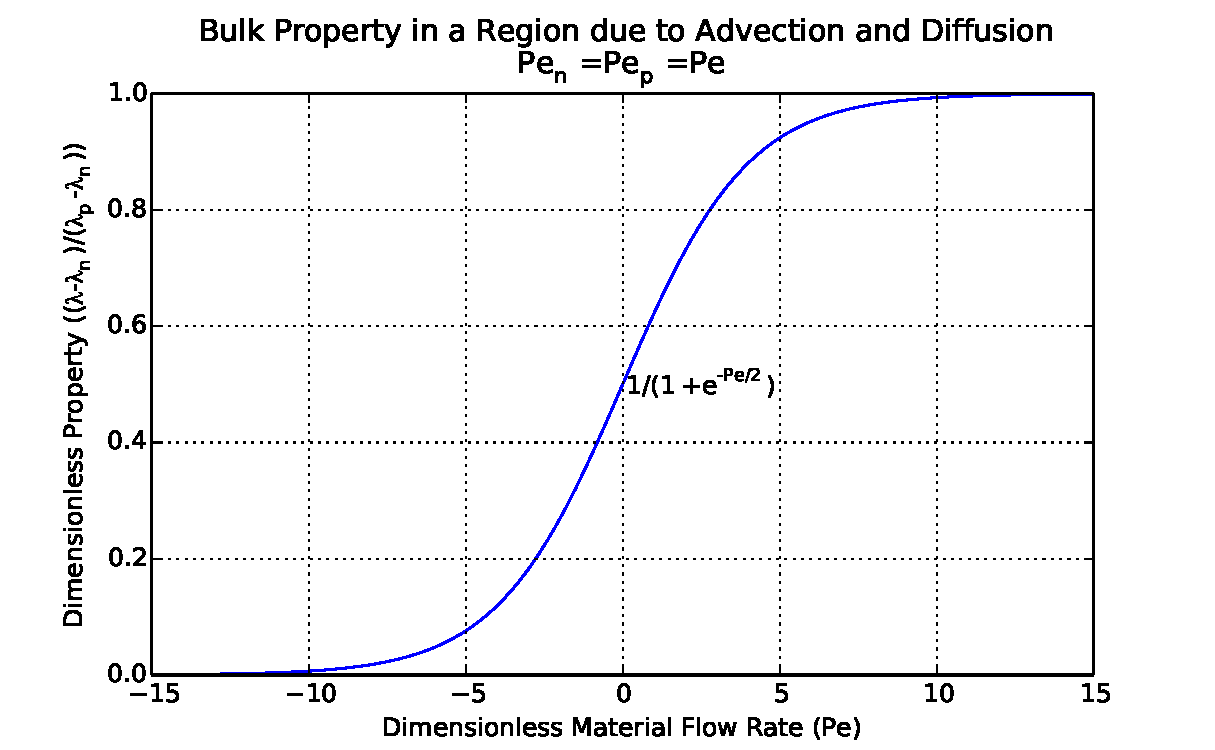
\includegraphics[width=0.9\linewidth]{3-AdvDiffRegion}%
  \caption{Property in the bulk of a region due to advection and diffusion}%
  \label{fig:AdvDiffRegion}
\end{figure}

\begin{figure}[htbp]
  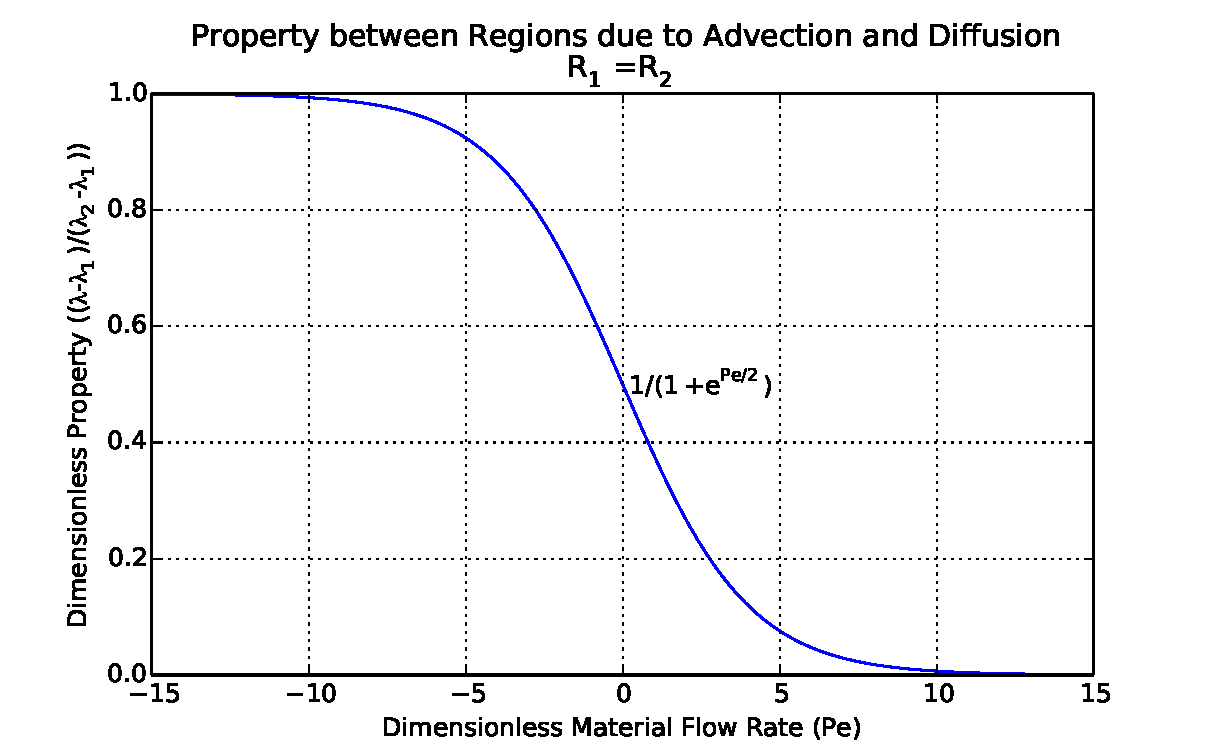
\includegraphics[width=0.9\linewidth]{3-AdvDiffInterface}%
  \caption{Property at the interface between regions due to advection and diffusion}%
  \label{fig:AdvDiffInterface}
\end{figure}

\autoref{eq:Mixing} can be used to provide the profile of the property between the centers of adjacent regions.  If we assume that the resistivity and cross-sectional area are uniform, \autoref{eq:Resistance1} implies that
\begin{equation}
  \frac{\s{gamma} - \s{gamma}_1}{\s{gamma}_2 - \s{gamma}_1} = \frac{\s{L}_1\group{1 + e^{-\s{Pe}/2}}}{\s{L}_1\group{1 + e^{-\s{Pe}/2}} + \s{L}_2\group{1 + e^{\s{Pe}/2}}}%
  \glsadd{_123}
\end{equation}
where $\s{L}_1$ is the length across region 1 and $\s{L}_2$ is the length across region 2.  If we vary the position of the interface while keeping the center-to-center distance the same (constant $\s{L} = (\s{L}_1 + \s{L}_2)/2$), we can express the value of the property as a function of position.
\begin{equation}
  \frac{\s{gamma} - \s{gamma}_1}{\s{gamma}_2 - \s{gamma}_1} = \frac{\s{x}[^star]\group{1 + e^{-\s{Pe}/2}}}{\s{x}[^star]\group{1 + e^{-\s{Pe}/2}} + \group{1 - \s{x}[^star]}\group{1 + e^{\s{Pe}/2}}}%
  \glsadd{_123}
\end{equation}
where $\s{x}[^star] = (\s{x} - \s{x}_1)/\s{L}$ is the dimensionless position between the first and second region as a function of~\s{x}, the absolute position of the interface.  This can be simplified to
\begin{equation}
  \label{eq:MixingProfile}
  \frac{\s{gamma} - \s{gamma}_1}{\s{gamma}_2 - \s{gamma}_1} = \frac{1}{1 + \group{\frac{1}{\s{x}[^star]} - 1}e^{\s{Pe}/2}}%
  \glsadd{_123}
\end{equation}
\autoref{fig:AdvDiffProfile} shows the resulting profile for various P\'eclet numbers (solid lines).  The profile is linear under pure diffusion ($\s{Pe} = 0$).  Otherwise, the profile is biased towards the property of the source.  The profile increases or decreases monotonically.  \autoref{eq:MixingProfile} reduces to \autoref{eq:MixingMidplane} when $\s{x}[^star] = 1/2$, as shown in the figure.

For comparison, Patankar~\cite{Patankar1980} provides the solution to the following general advection\slash{}diffusion equation under the condition of no material storage due to advection ($\mathrm{d}\s{I}/\mathrm{d}\s{x} = 0$) and no storage of the transported quantity due to combined advection and diffusion ($\mathrm{d}\dot{X}/\mathrm{d}\s{x} = 0$).  
\begin{equation}
  \dot{X} = \s{gamma}\s{I} - \frac{\s{A}}{\s{r}}\nabla\s{gamma}
\end{equation}
The equation has been refactored here under the assumption of uniform cross-sectional area.  The solution is
\begin{equation}
  \label{eq:PropertyProfile}
  \frac{\s{gamma} - \s{gamma}_1}{\s{gamma}_2 - \s{gamma}_1} = \frac{1 - e^{\s{Pe}\s{x}/\s{L}}}{1 - e^{\s{Pe}}}
  \glsadd{_123}
\end{equation}
where \s{L}~is the center-to-center distance between regions and \s{x}~is the position.  Note that this equation contains a numerical singularity in the case of pure diffusion ($\s{Pe} = 0$).  It matches \autoref{eq:MixingProfile} when $\s{x}[^star] = 1/2$, as shown by \autoref{fig:AdvDiffProfile}.  However, the model and the Patankar's solution are different at other positions.  This may be due to one of the following reasons: \begin{inparaenum}[(1)] \item the model is based on the requirement that the flow rate of the quantity out of one region is the flow rate into the other ($\dot{X}_{1\text{p}} + \dot{X}_{2\text{n}} = 0\glsadd{_pos}\glsadd{_neg}$ at the interface plane) whereas Patankar's solution is based on the requirement that there is no storage in a differential space around the interface ($\mathrm{d}\dot{X}/\mathrm{d}\s{x} = 0$) or \item the assumption of equal P\'eclet numbers (used in the derivation of \autoref{eq:MixingProfile} from \autoref{eq:Mixing}) is unreasonable\end{inparaenum}.  The P\'eclet number is extensive in nature (as mentioned previously), so it may not be appropriate to assume that it remains equal as the adjacent regions are resized.

\begin{figure}[htb]
  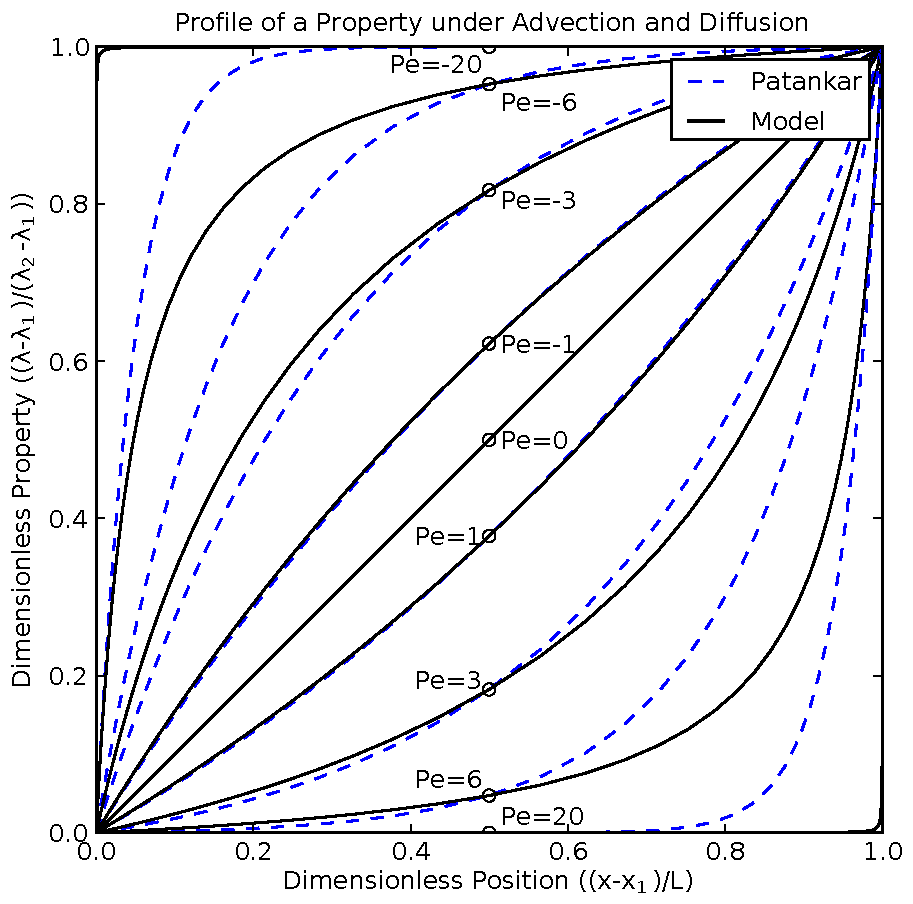
\includegraphics[width=0.75\linewidth]{3-AdvDiffProfile}%
  \caption[Profile of a property between regions due to advection and diffusion]{Center-to-center profile of a property between regions under advection and diffusion.  The model is equivalent to the Patankar's solution~\cite{Patankar1980} at the midplane ($\s{x} = \s{L}/2$)}%
  \label{fig:AdvDiffProfile}
\end{figure}

The previous evaluations are based on the condition that the flow rates of opposing transport equations are equal and opposite.  This is true at an interface between regions because the flow rate into one region is the rate out the other.  However, it is not necessarily the case across a region because the quantity may be stored within the region.  If we relax the previous assumption and provide the values of the driving property in the bulk of the region and at both boundaries, we can determine the rate of storage in a region:
\begin{equation}
  \label{eq:DiffusiveTransportStorage}
  \sum\dot{X} = \frac{\group{\s{gamma}[_neg] - \s{gamma}}\group{1 + e^{-\s{Pe}[_neg]/2}} + \group{\s{gamma}[_pos] - \s{gamma}}\group{1 + e^{\s{Pe}[_pos]/2}}}{\s{R}}
\end{equation}
If there is no advection, the rate of storage is proportional to the first-order approximation of the second derivative of the property over space:
\begin{equation}
  \sum\dot{X} = \frac{2}{\s{R}}\group{\s{gamma}[_neg] + \s{gamma}[_pos] - 2\s{gamma}}
\end{equation}

\autoref{tab:AdvDiff} shows the implications of \autoref{eq:DiffusiveTransportStorage}.  The third textual column and first graphic column indicate the rate of storage induced by positive or negative velocities and positive or negative property gradients under the condition of a linear property profile.  The fourth textual column and second graphic column indicate the concavity of the profile under the condition of no storage.  The curves are not to scale; \autoref{fig:AdvDiffProfile} gives the exact shape.  The boundary-to-boundary profile across a region must either match the first or second graphic column (and third or fourth textual column).  The center-to-center profile of a property must match the second graphic column---not the first since there is no storage at the interface between regions.

The first row of \autoref{tab:AdvDiff} indicates that if the property increases in the positive direction and the velocity is in the negative direction, either the conserved quantity is being removed from the region or the profile is concave up, or both.  If the gradient or the velocity is reversed, but not both, the quantity is stored instead or the concavity changes sign.  If both the gradient and the velocity are reversed, the storage regime and the concavity remain the same.  If the material flow is from higher to lower values of the property, the quantity is removed from the region; otherwise it is stored.  The concavity is always such that the gradient is lower on the side receiving the advection.

\begin{table}[hbt]
  \newcommand\C[1]{\multirow{2}*{#1}} % Hack to vertically align entries in a table
  \newcommand\G[1]{\C{\includegraphics[height=0.9cm]{#1}}} % Insert a graphic across two rows.
  \caption[Scenarios of \nname{1D} advection with diffusion]{Scenarios of \n{1D} advection with diffusion}%
  \label{tab:AdvDiff}%
  \begin{tabular}{ccccccccc}
    \toprule
    \textbf{Difference} & \C{$\land$} & \textbf{Velocity} & \C{$\Leftrightarrow$} & \textbf{Intake} & \C{$\lor$} & \textbf{Inflection} & \multicolumn{2}{c}{\textbf{Graphically:}} \\
    ($\Delta\s{gamma}$) & & (\s{phi}) & & ($\sum\dot{X}$) & & ($\Delta^2\s{gamma}$) & $\s{gamma}[_neg]\cdots\s{gamma}\cdots\s{gamma}[_pos]$ & or \\
    \midrule \addlinespace
    \C{$<0$} & & \C{$<0$} & & \C{$>0$} & & \C{$<0$} & \G{3-AdvDiffNegSlopeIn} & \G{3-AdvDiffNegSlopeDown} \\
    \\ \addlinespace
    \C{$<0$} & & \C{$>0$} & & \C{$<0$} & & \C{$>0$} & \G{3-AdvDiffNegSlopeOut} & \G{3-AdvDiffNegSlopeUp} \\
    \\ \addlinespace
    \C{$>0$} & & \C{$<0$} & & \C{$<0$} & & \C{$>0$} & \G{3-AdvDiffPosSlopeOut} & \G{3-AdvDiffPosSlopeUp} \\
    \\ \addlinespace
    \C{$>0$} & & \C{$>0$} & & \C{$>0$} & & \C{$<0$} & \G{3-AdvDiffPosSlopeIn} & \G{3-AdvDiffPosSlopeDown} \\
    \\ \addlinespace
    \bottomrule
  \end{tabular}%
\end{table}

The difference between the properties of adjacent regions is related to the flow rate between them by
\begin{equation}
  \s{gamma}_2 - \s{gamma}_1 = \dot{X}\group{\frac{\s{R}_1}{1 + e^{\s{Pe}/2}} + \frac{\s{R}_2}{1 + e^{-\s{Pe}/2}}}%
  \glsadd{_123}
\end{equation}
This follows from \autoref{eq:DiffusiveTransport3} (implemented for each region) and conservation of the transported quantity at the interface.  If the resistances are equal ($\s{R}_1 = \s{R}_2 = \s{R}$), then
\begin{equation}
  \label{eq:DiffusiveTransportTwoRegion}
  \s{R}\dot{X} = \s{gamma}_1 - \s{gamma}_2%
\end{equation}
which is typical diffusion.  This is applicable even if there is bulk material flow.  It confirms that the transport equation is a diffusion equation---only with upstream discretization so that advection can be properly determined.  Since the local gradient is affected by advection, the rate of diffusion is generally not proportional to the local gradient at the interface (given by \autoref{eq:MixingProfile}) but rather the average gradient between the centers of the regions.  Likewise, if there is no storage within a region along an axis and the P\'eclet numbers are equal at the boundaries, then
\begin{equation}
  \label{eq:DiffusiveTransportRegion}
  \s{R}\dot{X} = \s{gamma}[_neg] - \s{gamma}[_pos]
\end{equation}
where $\dot{X} = \dot{X}[_neg] = -\dot{X}[_pos]$.


\noindent\underline{\textbf{Discussion}}

The rate of advection is the product of the material flow rate and the amount of the quantity per unit of material (i.e., specific quantity).  In the case of material flow, this specific quantity is unity, since material is the quantity~\cite{Present1958}.  In the case of the translational advection, the specific quantity is velocity, the gradient of which also drives property.  For thermal advection, the specific quantity is temperature times specific entropy.  Temperature is the driving property for thermal diffusion, but specific entropy can be calculated from the temperature and concentration at the boundary.

\autoref{fig:AdvDiffFlow} shows the combined effects of advection and diffusion if the specific quantity is the same as the driving property for diffusion (e.g., translational advection).  The advection and diffusion are evaluated at the interface of two regions with the same resistances.  The property in the second region ($\s{gamma}_1\glsadd{_123}$) is arbitrarily five times the property in the first region ($\s{gamma}_2$).  The rate of diffusion is constant (in dimensionless units), as predicted by \autoref{eq:DiffusiveTransportTwoRegion}.  As advection is initially increased, the property at the interface becomes nearly the mean of the properties of the regions.  The actual rate of advection is quite different from the ideal rate given by the upstream scheme.  A correction must be applied because the property at the interface is not the property of the upstream region.  Here, that correction is called \emph{\n{irreversible advection}} because this part of advection has been affected by the irreversible process of diffusion.   As the magnitude of the P\'eclet number becomes large, the irreversible advection becomes negligible because the interface takes on the property of the upstream region.

\begin{figure}[htbp]
  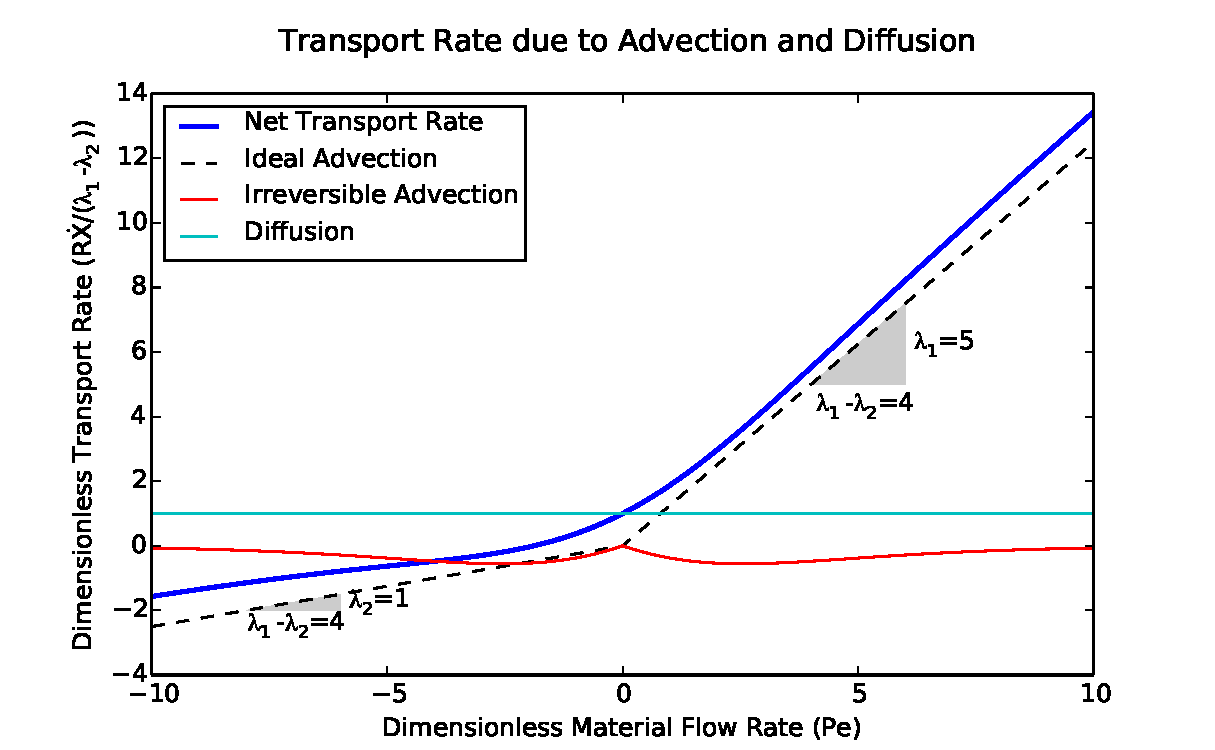
\includegraphics[width=0.9\linewidth]{3-AdvDiffFlow}%
  \caption{Transport rate of a conserved quantity under mixed advection and diffusion}%
  \label{fig:AdvDiffFlow}
\end{figure}

So far, we have evaluated the transport equations along one axis.  It is possible to implement \autoref{eq:DiffusiveTransport3} for all three dimensions simultaneously as long as the coordinate system is aligned with the principle axes of transport (Assumption \ref{itm:AssumeAligned} in the beginning of \autoref{sec:Transport}).   When the coordinate system is not aligned with the principle axes of transport, the model is subject to false diffusion like most methods of upstream discretization~\cite{Patankar1980}. 

Although the transport equation (\ref{eq:DiffusiveTransport3}) contains an exponential, it is not equivalent to the exponential scheme.  The exponential scheme is derived by \begin{inparaenum}[(1)]\item solving the advection\slash{}diffusion equation analytically for the profile of the driving property under the assumption of no storage and \item reintroducing the solution into the advection\slash{}diffusion equation without that original assumption\end{inparaenum}~\cite{Patankar1980, Majumdar2005}.  It results in a solution that is numerically singular unless there is advection.  The main argument against the exponential scheme---that it is computationally expensive---also applies to the transport equation used here.  However, the transport equation is used within a framework that \begin{inparaenum}[(1)]\item does not require a large number of regions for convergence and \item eliminates all nonlinear systems of equations\end{inparaenum}.  The argument may also be out of context now because it dates back to at least 1980~\cite{Patankar1980}, when computational resources were relatively limited.

As demonstrated in \autoref{sec:Exchange}, the traditional material derivative is the rate of diffusion.  This holds for transport as well.  The total rate of transport (\autoref{eq:Transport}) can be expanded with the rates of advection and diffusion from Equations \ref{eq:AdvectiveTransport} and \ref{eq:DiffusiveTransport2}:
\begin{equation}
  \dot{X}[_i]= \dot{N}[_i]\diffp{\s{X}}{\s{N}}[_i] + \Diff{\s{X}}{\s{t}}[_i]
\end{equation}
We will take this to be the positive side of the region so that the derivatives are in the positive direction and assume that the current is advective ($\dot{N} = -\s{phi}\s{A}\s{rho} =  -\s{phi}\partial\s{N}/\partial\s{x}$).  Then, dropping the subscripts,
\begin{equation}
  \dot{X} = -\s{phi}\diffp{\s{X}}{\s{x}} + \Diff{\s{X}}{\s{t}}
\end{equation}
Since the model uses a Eulerian perspective, the total transport rate \dot{X} is actually a partial derivative in the form of $\partial\s{X}/\partial\s{t}$.  After rearranging,
\begin{equation}
  \Diff{\s{X}}{\s{t}} = \diffp{\s{X}}{\s{t}} + \s{phi}\diffp{\s{X}}{\s{x}}
\end{equation}
Usually the scalar property in the material derivative is intensive (e.g., \s{gamma}, the driving property for diffusion).  Dividing by $\partial\s{X}/\partial\s{gamma}$,
\begin{equation}
  \Diff{\s{gamma}}{\s{t}} = \diffp{\s{gamma}}{\s{t}} + \s{phi}\diffp{\s{gamma}}{\s{x}}
\end{equation}
and generalizing to three dimensions,
\begin{equation}
  \Diff{\s{gamma}}{\s{t}} = \diffp{\s{gamma}}{\s{t}} + \boldsymbol{\s{phi}\cdot\nabla}\s{gamma}
\end{equation}
This is the definition of the material derivative~\cite{Bird2007}.

% Positive resistivity is characterized by irreversibility, damping, mixing, entropy production, and exergy destruction.  It corresponds to a real, stable situation where a distribution becomes uniform by exponential decay over time.  Zero resistivity is characterized by reversibility, zero damping, the maintenance of separation, and the absence of entropy production or exergy destruction.  It corresponds an ideal, marginally stable situation where distribution persists, because advection is perfectly balanced by transport around the region in the opposite direction.  Negative resistivity corresponds to a unstable situation where a distribution become less uniform by exponential growth over time.  It is physically impossible due to the second law of thermodynamics.


\subsection{Material Transport}
\label{sec:MaterialTransport}


As stated by James Clerk Maxwell, ``Mass transfer is due partly to the motion of translation and partly to that of agitation''~\cite{Burghardt2013}.  Here, the ``translation'' component of mass transfer is called material advection.  It is also called migration in the context of chemical engineering and drift in the context of solid state physics (\autoref{sec:Ohms}).  The ``agitation'' component is diffusion.  In accordance with Maxwell's statement, the total current into the region through boundary~\s{i} is the sum of the advective (``translation'') and diffusive (``agitation'') currents:
\begin{equation}
  \label{eq:MaterialTransport}
  \boxed{\dot{N}[_i]= \dot{N}\sub{_A}[_i] + \dot{N}\sub{_D}[_i]}
\end{equation}
This is simply \autoref{eq:Transport} where the transported quantity~(\s{X}) is material~(\s{N}).
% The total current can be written as
% \begin{equation}
%   \dot{N}[_i] = \frac{\s{k}\s{A}}{\s{zeta}\s{L}}\group{\s{rho}[_i] - \s{rho}}\group{1 + e^{\mp\s{zeta}\s{phi}[_perp]\s{L}/2\s{k}}} \pm \s{rho}[_i]\s{A}\group{\frac{\s{L}\s{beta}\dot{mPhi}\sub{_D}[_perp][_i]}{\s{k}\s{A}\group{1 + e^{\mp\s{beta}\s{M}\s{phi}[_perp]/2\s{k}\s{A}}}} + \s{phi}[_perp]}
% \end{equation}
% If there is zero net current and zero dynamic compressibility, then
% \begin{equation}
%   \s{rho} = \s{rho}[_i]\group{1 \pm \frac{\s{zeta}\s{L}}{\s{k}\group{1 + e^{\mp\s{zeta}\s{phi}[_perp]\s{L}/2\s{k}}} }\s{phi}[_perp]}
% \end{equation}


\subsubsection{Advection}

The general advection equation (\ref{eq:AdvectiveTransport}) reduces to an identity when the transported quantity~(\s{X}) is the amount of material~(\s{N}).  Instead, the amount of material in that equation is first replaced by the position into the region along the axis of transport.  Then, the partial derivative $\partial\s{X}/\partial\s{N}$ becomes $\partial\s{N}/\partial\s{x}$ or $\s{rho}\s{A}$.  The current \dot{N} becomes $\dot{x}$ or velocity directed into the region ($\pm\s{phi}$).  Therefore,
\begin{equation}
  \label{eq:MaterialAdvection}
  \boxed{\dot{N}\sub{_A}[_i] = \pm \s{phi}\sub{_perp}[_i]\s{rho}[_i]\s{A}[_i]}
\end{equation}
where the positive of $\pm$ is for the negative boundaries and the negative is for positive boundaries.  The subscript $\perp$ indicates the component of velocity normal to the boundary.  The value of the velocity will be established by \autoref{eq:NormalDiffusion}, but for now, it is considered known.



\subsubsection{Diffusion}
\label{sec:MaterialDiffusion}

The rate of material diffusion follows from Equations \ref{eq:DiffusiveTransport4} and \ref{eq:Peclet3}.  Material~(\s{N}) is the transported quantity~(\s{X}) and concentration~(\s{rho}) is the driving property~(\s{gamma}).
\begin{equation}
  \label{eq:MaterialDiffusion}
  \boxed{\s{zeta}\dot{N}\sub{_D}[_i] = \frac{\s{k}[_i]\s{A}[_i]}{\s{L}[_i]}\group{\s{rho}[_i] - \s{rho}}\group{1 + e^{\mp\s{zeta}\s{V}\s{phi}\sub{_perp}[_i]/2\s{k}[_i]\s{A}[_i]}}}
\end{equation}
where \dot{N}[_i] is the diffusive current into the region through boundary~\s{i}.  The volume~(\s{V}) is the volume of the phase.  However, the area~(\s{A}) is the cross-sectional area of the region along the axis of transport and \s{L}~is the length of the same.  The variable~\s{rho}[_i]~is the concentration or volumic amount of material at the boundary.   This concentration is not molar concentration or number concentration; it can be determined independently for each species.   The concentration in the region may be considered known, since it is a state of the material balance (\autoref{sec:BasicMaterialBalance}).  If a species is isochoric in a phase (e.g., liquid \n{H2O}), it will not diffuse.

The material resistivity, \s{zeta}, can be estimated from the generalized definition of resistivity (\autoref{eq:Resistivity}):
\begin{equation}
  \label{eq:MaterialResistivity}
  \boxed{\s{zeta} = \frac{3\s{tau}}{\s{lambda}^2}}
\end{equation}
The material resistivity is the reciprocal of self diffusivity, which is the ability of trace particles of a species to diffuse through other particles of the same species~\cite{Present1958}.  This is the essence of \autoref{eq:MaterialDiffusion}; it describes the rate of diffusion through an advected stream of particles of the same type.

The material transport equation is closely related to Fick's law\label{mark:FicksLaw}.  If we assume that the bulk velocity (and advective current) is zero along the axis of transport and the area factor (\s{k}[_i]) is unity, the rate of material diffusion (\autoref{eq:MaterialDiffusion}) reduces to
\begin{equation}
  \s{zeta}\dot{N}[_i] = 2\frac{\s{A}[_i]}{\s{L}[_i]}\group{\s{rho}[_i] - \s{rho}}
\end{equation}
If the concentration gradient is uniform, there is no material storage due to diffusion ($\dot{N}[_neg] = -\dot{N}[_pos] = \s{A}\s{J}$).  In that case, we can combine the negative- and positive-side equations as:
\begin{equation}
  \s{zeta}\s{J} = \frac{\s{rho}[_neg] - \s{rho}[_pos]}{\s{L}}
\end{equation}
Taking the limit as length goes to zero and generalizing to three dimensions,
\begin{equation}
  \s{zeta}\mathbf{\s{J}} = -\mathbf{\nabla}\s{rho}
\end{equation}
which is Fick's first law~\cite{Bird2002, Burghardt2013, Liggett1994, Wesselingh2000, Bockris2000, Taylor1993}.%\cite[p.~515]{Bird2002}, \cite[p.~426]{Liggett1994}

Fick's law also appears in other forms in the literature.  In theory, any intensive thermodynamic property could be used as long as it is sufficient to fix the thermodynamic state of the species given its temperature.  The choice affects the transport rate and thus the resistivity must be set properly, but it will not affect the equilibrium.  All of the intensive thermodynamic properties are uniform between two regions in thermodynamic equilibrium (aside from outside forces), and the equilibrium point is determined by the conservation equations (Sections~\ref{sec:BasicConservation} and \ref{sec:DetailedConservation}).

Since the species has constant specific mass, we can write Fick's law in terms of density~\cite{Burghardt2013, Bejan2006}:
\begin{equation}
  \s{m}\s{zeta}\timessep\s{J} = -\nabla\group{\s{mrho}}
\end{equation}
If the species exists in small amounts within an otherwise uniform mixture, the extensive volume (in $\s{rho} = \s{N}/\s{V}$) can be replaced by the total amount or mass of the phase.  For mole fractions, this is~\cite{Majumdar2005, Burghardt2013, Incropera2002, Taylor1993}
\begin{equation}
  \frac{\s{V}\s{zeta}}{\s{N}[_tot]}\timessep\s{J} \approx -\nabla\group{\s{N}/\s{N}[_tot]}
\end{equation}
where \s{N}~is the number of particles of the transported species and \s{N}[_tot]~is the total number of particles in the phase.  For mass fractions, we can write this as~\cite{Majumdar2005, Burghardt2013, Incropera2002, Taylor1993}
\begin{equation}
  \frac{\s{m}\s{V}\s{zeta}}{\s{M}[_tot]}\timessep\s{J} \approx -\nabla\group{\s{M}/\s{M}[_tot]}
\end{equation}
We can also write Fick's law in terms of partial pressure~\cite{Burghardt2013}:
\begin{equation}
  \diffp{\s{p}}{\s{rho}}[_T]\s{zeta}\timessep\s{J} = -\nabla\s{p}
\end{equation}
For ideal gases, this is
\begin{equation}
  \s{T}\s{zeta}\timessep\s{J} = -\nabla\s{p}
\end{equation}
Since the material resistivity is roughly the base resistivity factor divided by specific volume (see \autoref{eq:MaterialResistivity}), we can write this as (again, assuming ideal gas)
\begin{equation}
  \s{alpha}\timessep\s{J} = -\nabla\ln\s{p}
\end{equation}
For an isothermal ideal gas, \autoref{eq:GibbsFunction} implies that
\begin{equation}
  \label{eq:FicksLawGibbsIdealGas}
  \s{T}\s{alpha}\timessep\s{J} = -\nabla\s{g}
\end{equation}
Since \s{alpha}~is only dependent on temperature and fixed properties (specific mass and particle diameter), chemical potential (here, \s{g}) may be preferred as the driving property for material diffusion.  The magnitude of the diffusion rate in the previous forms of Fick's law is coupled to the concentration, which is affected over time by the diffusion itself (if storage is allowed).  We can also express Fick's law in terms of chemical potential for species that are not ideal gases~\cite{Matuszak2006}:
\begin{equation}
  \s{zeta}\group{\diffp{\s{g}}{\s{rho}}}\timessep\s{J} = -\nabla\s{g}
\end{equation}
If temperature is uniform, this is
\begin{equation}
  \frac{\s{zeta}}{\s{rho}}\diffp{\s{p}}{\s{rho}}[_T]\s{J} = -\nabla\s{g}
\end{equation}
If the species is an ideal gas, this again reduces to \autoref{eq:FicksLawGibbsIdealGas}.  The model uses concentration as the driving property for diffusion because the boundary pressure is needed for the momentum balance (\autoref{sec:TranslationalBalance}) and concentration is available as a dynamic property anyway.  Pressure is an explicit function of concentration as long as the species is compressible (\autoref{eq:VirialBerlin1}), but pressure cannot generally be expressed as a function of specific Gibbs energy (except in special cases).

% In the literature within the field of \np{PEMFC}~\cite{Weber-Review2004}, the transport process is often described with a viscous flow equation such as Darcy's law and $\n{n}[_spec] - 1$ repetitions of an equation consisting of momentum, Maxwell-Stefan diffusion, and Knudsen diffusion terms.  However, this approach is not rigorous in terms of energy.  Weber and Newman~\cite{Weber2005} note that the typical modeling approach, the dusty-gas model, can lead to a singular matrix.


\subsection{Normal Translational Advection and Nonequilibrium Compression}
\label{sec:NormalTransport}

In the previous section, we treated the normal component of velocity at a boundary ($\s{phi}\sub{_perp}[_i]$) as if it were known.  In this section, it is related to the velocity within the region by the effect of bulk or volume viscosity.  This entails a set of advection\slash{}diffusion equations for the normal component of translational momentum.

The normal force on boundary~\s{i} is due to the sum of the advective and diffusive forces:
\begin{equation}
  \label{eq:NormalForce}
  \dot{mPhi}\sub{_perp}[_i] = \dot{mPhi}\sub{_A}[_perp][_i] + \dot{mPhi}\sub{_D}[_perp][_i]
\end{equation}
This follows the form of \autoref{eq:Transport} where the transported quantity~(\s{X}) is the normal component of translational momentum~(\s{mPhi}).  The advective component is often called dynamic pressure (or force in this case) and the diffusive component may be called nonequilibrium pressure~\cite{Meier2005}.  Thermodynamic pressure is excluded here, but it is included in the translational momentum balance (\autoref{eq:TranslationalBalance}).


\subsubsection{Advection}
\label{sec:NormalAdvection}

The advective normal force follows from \autoref{eq:AdvectiveTransport}.
\begin{equation}
  \label{eq:NormalAdvection}
  \dot{mPhi}\sub{_A}[_perp][_i] = \dot{N}[_i]\s{m}\s{phi}\sub{_perp}[_i]
\end{equation}
where $\s{phi}\sub{_perp}[_i]$~is the normal velocity at boundary~\s{i}.  Since this equation applies to each configuration separately, the specific mass at the boundary (\s{m}[_i]) is the same as the specific mass in the region~(\s{m}) and the subscript is not necessary.  The current (\dot{N}[_i]) includes advective and diffusive parts according to \autoref{eq:MaterialTransport}.


Using Equations \ref{eq:MaterialTransport} and \ref{eq:MaterialAdvection}, the advective normal force can be expanded as
\begin{equation}
  \label{eq:NormalAdvection2}
  \dot{mPhi}\sub{_A}[_perp][_i] = \s{m}\dot{N}\sub{_D}[_i]\s{phi}\sub{_perp}[_i] \pm \s{m}\s{rho}[_i]\s{A}[_i]\s{phi}\sub{_perp}[_i]^2
\end{equation}
where \s{x}~is the position along the axis of transport.  The second term on the right side is closely related to the dynamic pressure\label{mark:DynamicPressure} ($\s{m}\s{rho}\s{phi}^2/2$) usually expressed in \np{PDE}.  However, the essence of dynamic pressure---the advection of translational momentum---is implemented directly instead of using a discrete approximation to the traditional \np{PDE}.  Assuming that the specific mass and concentration are constant, the derivative of the traditional dynamic pressure is $\s{m}\s{rho}\s{phi}\partial\s{phi}$.  The force that results over a distance $\mathrm{d}\s{x}$ is $\s{M}\s{phi}\partial\s{phi}/\partial\s{x}$.  The first-order discrete approximation is $\s{M}\s{phi}\Delta\s{phi}/\s{L}$; its implementation would yield a boundary force of $\pm\s{m}\s{rho}\s{A}\s{phi}[_perp]\s{phi}\sub{_perp}[_i]$ in the nomenclature of \autoref{eq:NormalAdvection2}.  This is only an approximation to the force due to material advection.  It does not guarantee conservation of momentum at the boundary, since adjacent regions may have different normal velocities (\s{phi}[_perp]).  This is troubling because the lack of conservation can lead to artificial instabilities.  The actual force---the one used in the model---involves the product of density, advective current, and velocity precisely at the interface (second term on the right side of \autoref{eq:NormalAdvection2}).


\subsubsection{Diffusion}
\label{sec:NormalDiffusion}

The diffusive normal force follows from \autoref{eq:DiffusiveTransport4} with the component of velocity normal to the boundary (\s{phi}[_perp]) as the diffusion-driving property~(\s{gamma}):
\begin{equation}
  \label{eq:NormalDiffusion}
  \boxed{\s{beta}\dot{mPhi}\sub{_D}[_perp][_i] = \frac{2\s{k}[_i]\s{A}[_i]}{\s{L}[_i]}\Group{\s{phi}\sub{_perp}[_i] - \s{phi}[_perp]\frac{\s{V}}{\s{V}[_tot]}}}
\end{equation}
This is the force due to nonequilibrium compression.  The form of the equation departs from the general equation (\ref{eq:DiffusiveTransport4}) in two ways, which will be explained.

The first departure from \autoref{eq:DiffusiveTransport4} is that the porosity, $\s{V}/\s{V}[_tot]$, has been applied to the velocity in the region to account for the presence of other phases.  If multiple phases are present in the region, only part of the boundary is open to material transport in any one of the phases.  Yet the material advection equation (\ref{eq:MaterialAdvection}) assumes that the velocity is uniform over the boundary.  The porosity is an attempt to account for this inaccuracy.  The fraction of open area at the boundary (e.g., areal porosity) is assumed to be the fraction of open volume in the region (e.g., volumetric porosity).  The porosity cannot be introduced directly in the material advection equation because neighboring regions may have different volume fractions.  If it were, material conservation would be violated at the boundary.  By placing the porosity in \autoref{eq:NormalDiffusion}, the neighboring regions must agree on the fraction of open area at their common boundary.

The second departure is that no upstream discretization has been applied in \autoref{eq:NormalDiffusion}.  The velocity at the boundary is assumed to be zero for the sake of calculating the P\'eclet number at the boundary (\autoref{eq:Peclet3}).  A nonzero P\'eclet number would imply that the velocity at the boundary anticipates the propagation of the velocity property itself from the center of the region to the boundary.  This seems to be a violation of physics.


The variable~\s{beta} represents the \emph{\n{dynamic compressibility}} which describes the extent to which a non-equilibrium normal force causes or requires transient compression.  It can be estimated from the generalized definition of resistivity (\autoref{eq:Resistivity}):
\begin{equation}
  \label{eq:DynamicCompressibility}
  \boxed{\s{beta} = \frac{3\s{tau}}{\s{lambda}^2\s{rho}\s{m}}}
\end{equation}
Dynamic compressibility is the reciprocal of bulk viscosity as a dynamic (rather than kinematic) viscosity.  Although bulk viscosity differs from shear viscosity~\cite{Karim1952, Schetz1996, Rah1999, Liggett1994}, % \cite[p.~25]{Liggett1994}
the same initial estimate is used.  Dynamic compressibility is different from compressibility, which is $-\group{\partial\s{v}/\partial\s{p}}/\s{v}$.


\subsection{Transverse Translational Advection and Friction}
\label{sec:TransverseTransport}

The force on boundary~\s{i} transverse to the surface is due to the sum of the advective and diffusive forces:
\begin{equation}
  \label{eq:TransverseForce}
  \dot{mPhi}\sub{_para}[_i] = \dot{mPhi}\sub{_A}[_para][_i] + \dot{mPhi}\sub{_D}[_para][_i]
\end{equation}
This follows the form of \autoref{eq:Transport} where the transported quantity~(\s{X}) is a component of translational momentum transverse to the boundary (\s{mPhi}[_para]).  This equation is implemented twice---once for each transverse direction.


\subsubsection{Advection}

Translational momentum is advected according to the generalized advective transport equation (\ref{eq:AdvectiveTransport}).  In terms of the present variables, this is
\begin{equation}
  \label{eq:TransverseAdvection}
  \dot{mPhi}\sub{_A}[_para][ ][_i] = \dot{N}[_i]\s{m}\s{phi}\sub{_para}[ ][_i]
\end{equation}
where $\s{phi}\sub{_para}[ ][_i]$ is a component of velocity transverse to boundary~\s{i}.  Since this equation applies to each configuration separately, the specific mass at the boundary (\s{m}[_i]) is the same as the specific mass in the region~(\s{m}) and the subscript is not necessary.  The current (\dot{N}[_i]) includes advective and diffusive parts according to \autoref{eq:MaterialTransport}.


\subsubsection{Diffusion}

The friction or shear force along a boundary follows the generalized diffusive transport equation (\ref{eq:DiffusiveTransport4}) with an adjustment factor.  The  driving property is a transverse component of velocity (\s{phi}[_para]) aligned with the shear force.
\begin{equation}
  \label{eq:ShearForce}
  \boxed{\s{eta}\dot{mPhi}\sub{_D}[_para][ ]{_i}\sup{^prime} = \frac{\s{Nu}[_Phi]\s{k}[_i]\s{A}[_i]}{\s{L}[_i]}\group{\s{phi}\sub{_para}[ ]{_i} - \s{phi}[_para]}\group{1 + e^{\mp\s{eta}\s{M}\s{phi}\sub{_perp}[_i]/2\s{k}[_i]\s{A}[_i]}}}
\end{equation}
where $\dot{mPhi}\sub{_D}[_para][ ]{_i}\sup{^prime}$ is the shear force.  The reason for the prime superscript will be discussed below.  The boundary velocity ($\s{phi}\sub{_para}[ ][_i]$) is an effective velocity.  Its usage does not imply that the velocity is uniform over the boundary (which would generally lead to discontinuities in the velocity at the edges of the boundary).  Unlike the normal diffusive force (\autoref{eq:NormalDiffusion}), the shear force uses upstream discretization.  The associated P\'eclet number is based on the normal component of velocity at the boundary ($\s{phi}\sub{_perp}[_i]$).

The fluidity, \s{eta}, can be estimated from the generalized definition of resistivity (\autoref{eq:Resistivity}):
\begin{equation}
  \label{eq:Fluidity}
  \boxed{\s{eta} = \frac{3\s{tau}}{\s{lambda}^2\s{rho}\s{m}}}
\end{equation}
Fluidity is the reciprocal of shear viscosity as a dynamic (rather than kinematic) viscosity.  If two adjacent regions have zero fluidity~(\s{eta}), the parallel components of their velocities are equal and the number of states is reduced by two.  Translational momentum will flow between the regions without loss.

The additional variable~\s{Nu}[_Phi] is the shear shape factor or the \emph{\n{translational Nusselt number}}---the analog of the traditional or thermal Nusselt number for the diffusion of translational momentum.  It allows the shear force equation (\ref{eq:ShearForce}) to be used at relatively coarse levels of discretization.  It is defined as the ratio of the average inward velocity gradient along the perimeter divided by the difference between the boundary velocity and the bulk velocity over the distance from the boundary to the center of the region:
\begin{equation}
  \label{eq:TranslationalNusselt}
  \s{Nu}[_Phi] \equiv \left.\diffp{\s{phi}[_para]}{\s{x}}[_i]\middle/2\frac{\s{phi}\sub{_para}[ ][_i] - \s{phi}[_para]}{\s{L}[_x]}\right.
\end{equation}
\autoref{tab:TranslationalNusselt} summarizes the shape factor or the translational Nusselt number given two assumptions: \begin{inparaenum}[(1)]\item the material concentration is uniform and \item the boundary velocities are uniform around the perimeter\end{inparaenum}.  The first assumption implies that the bulk, mass-average velocity is equal to the volume-average velocity.  The shape factor is one in a \nfirst{2D} case (where no force is applied the third dimension, e.g., its length is infinite) with a linear velocity profile.  The velocity changes from the boundary velocity to the bulk velocity (solid blue vertical line) in half of the distance between the boundaries.  The shape factor is two in a \nfirst{2D} case with a piecewise linear velocity profile.  Then, the velocity changes from the boundary velocity to the bulk velocity in one fourth of the distance between the boundaries.  The shape factor is three in a \nfirst{3D} case with a piecewise linear velocity profile because the volume of a pyramid is one third the product of its base area and height.  The shape factor is four if the flow is fully developed and laminar (Hagen-Poiseuille flow, discussed below).  If the flow is turbulent, the shape factor is greater than four; the velocity gradient at the wall is greater than for laminar flow.

\begin{table}[hbt]
  \newcommand\C[1]{\multirow{4}*{#1}} % Hack to vertically align entries in a table
  \newcommand\G[1]{\C{\includegraphics[height=2cm]{#1}}} % Insert a graphic across multiple rows.
  \caption{Values of the translational Nusselt number}%
  \label{tab:TranslationalNusselt}%
  \begin{tabular}{cccl}
    \toprule
    \textbf{Shape factor} & \multirow{2}*{\textbf{Profile}} & \textbf{Number of} & \multirow{2}*{\textbf{Description}} \\
    (\s{Nu}[_Phi]) &  & \textbf{dimensions} &  \\
    \midrule \addlinespace
    \C{1} & \G{3-ShapeFactorCouette} & \C{2} & \C{Couette flow (linear)} \\
    \\ \\ \\\addlinespace
    \C{2} & \G{3-ShapeFactorPiecewise2D} & \C{2} & \C{Piecewise linear (triangle)} \\
    \\ \\ \\\addlinespace
    \C{3} & \G{3-ShapeFactorPiecewise3D} & \C{3} & \C{Piecewise linear (pyramid)} \\
    \\ \\ \\\addlinespace
    \C{4} & \G{3-ShapeFactorLaminar} & \C{3} & \C{Laminar fully developed (parabola)} \\
    \\ \\ \\\addlinespace
    \C{$>4$} & \G{3-ShapeFactorTurbulent} & \C{3} & \C{Turbulent (higher order)} \\
    \\ \\ \\\addlinespace
    \bottomrule
  \end{tabular}%
\end{table}

The model does not directly use the shear force equation (\ref{eq:ShearForce}) because the forces apply torques and the model is based on the assumption that rotational momentum is not stored (see \autoref{sec:RotationalConservation}).  This is the reason for the prime superscript in the shear force equation (\ref{eq:ShearForce}).  The conservation of rotational momentum (\autoref{eq:RotationalConservationX}) gives one of the four equations required for the four boundaries around the perimeter of the region along the x~axis.  The first of the remaining three equations requires that the total force in the y direction is the force determined by the y-direction shear force equations:
\begin{equation}
  \boxed{\dot{mPhi}\sub{_y}[_neg][_z] + \dot{mPhi}\sub{_y}[_pos][_z] = \dot{mPhi}\sub{_y}[_neg][_z]\sup{^prime} + \dot{mPhi}\sub{_y}[_pos][_z]\sup{^prime}}
\end{equation}
Similarly in the z direction:
\begin{equation}
  \boxed{\dot{mPhi}\sub{_z}[_neg][_y] + \dot{mPhi}\sub{_z}[_pos][_y] = \dot{mPhi}\sub{_z}[_neg][_y]\sup{^prime} + \dot{mPhi}\sub{_z}[_pos][_y]\sup{^prime}}
\end{equation}
The final equation requires that the torque applied to the y boundaries opposes the torque applied to the z boundaries to the same extent calculated by the shear force equations:
\begin{equation}
  \boxed{\group{\dot{mPhi}\sub{_z}[_neg][_y] - \dot{mPhi}\sub{_z}[_pos][_y]}\s{L}[_z] + \group{\dot{mPhi}\sub{_y}[_neg][_z] - \dot{mPhi}\sub{_y}[_pos][_z]}\s{L}[_y] =  \group{\dot{mPhi}\sub{_z}[_neg][_y]\sup{^prime} - \dot{mPhi}\sub{_z}[_pos][_y]\sup{^prime}}\s{L}[_z] + \group{\dot{mPhi}\sub{_y}[_neg][_z]\sup{^prime} - \dot{mPhi}\sub{_y}[_pos][_z]\sup{^prime}}\s{L}[_y]}
\end{equation}
Similar equations apply to the perimeters around the y and z axes.  The translational advection equation (\ref{eq:TransverseAdvection}) is applied directly; we assume that it interacts with the center of the region and produces no torque.

% If we use the shear force equation (\ref{eq:ShearForce}) and assume that the cross-wise components of velocity are zero, we can write the three new shear force equations as
% \begin{subequations}
%   \begin{equation}
%     \label{eq:ShearForceY}
%     \dot{mPhi}\sub{_y}[_neg][_z] + \dot{mPhi}\sub{_y}[_pos][_z] = \frac{2\s{Nu}[_Phi]\s{A}[_y]}{\s{eta}\s{L}[_y]}\group{\s{phi}\sub{_y}[_neg][_z] + \s{phi}\sub{_y}[_pos][_z] - 2\s{phi}[_y]}
%   \end{equation}
%   \begin{equation}
%     \label{eq:ShearForceZ}
%     \dot{mPhi}\sub{_z}[_neg][_y] + \dot{mPhi}\sub{_z}[_pos][_y] = \frac{2\s{Nu}[_Phi]\s{A}[_z]}{\s{eta}\s{L}[_z]}\group{\s{phi}\sub{_z}[_neg][_y] + \s{phi}\sub{_z}[_pos][_y] - 2\s{phi}[_z]}
%   \end{equation}
%   \begin{equation}
%     \label{eq:ShearForceCounter}
%     \group{\dot{mPhi}\sub{_z}[_neg][_y] - \dot{mPhi}\sub{_z}[_pos][_y]}\s{L}[_y] + \group{\dot{mPhi}\sub{_y}[_neg][_z] - \dot{mPhi}\sub{_y}[_pos][_z]}\s{L}[_z] = \frac{2\s{Nu}[_Phi]}{\s{eta}}\Group{\group{\s{phi}\sub{_z}[_neg][_y] - \s{phi}\sub{_z}[_pos][_y]}\s{A}[_y] + \group{\s{phi}\sub{_y}[_neg][_z] - \s{phi}\sub{_y}[_pos][_z]}\s{A}[_z]}
%   \end{equation}
% \end{subequations}
% Equations~\ref{eq:ShearForceY} and \ref{eq:ShearForceZ} involve second-order differences, but \autoref{eq:ShearForceCounter} only involves first-order differences.

In three dimensions, this method involves a system of twelve equations which can be solved for the twelve shear forces (two for each of six boundaries).  The shear forces in the x direction are:
\begin{subequations}
  \label{eq:ForceMap}
  \begin{align}
    4\dot{mPhi}\sub{_y}[_neg][_x] &= 3\dot{mPhi}\sub{_y}[_neg][_x]\sup{^prime} + \dot{mPhi}\sub{_y}[_pos][_x]\sup{^prime} + \frac{\s{L}[_x]}{\s{L}[_y]}\group{\dot{mPhi}\sub{_x}[_neg][_y]\sup{^prime} - \dot{mPhi}\sub{_x}[_pos][_y]\sup{^prime}} \\
    4\dot{mPhi}\sub{_y}[_pos][_x] &= 3\dot{mPhi}\sub{_y}[_pos][_x]\sup{^prime} + \dot{mPhi}\sub{_y}[_neg][_x]\sup{^prime} + \frac{\s{L}[_x]}{\s{L}[_y]}\group{\dot{mPhi}\sub{_x}[_pos][_y]\sup{^prime} - \dot{mPhi}\sub{_x}[_neg][_y]\sup{^prime}} \\
    4\dot{mPhi}\sub{_z}[_neg][_x] &= 3\dot{mPhi}\sub{_z}[_neg][_x]\sup{^prime} + \dot{mPhi}\sub{_z}[_pos][_x]\sup{^prime} + \frac{\s{L}[_x]}{\s{L}[_z]}\group{\dot{mPhi}\sub{_x}[_neg][_z]\sup{^prime} - \dot{mPhi}\sub{_x}[_pos][_z]\sup{^prime}} \\
    4\dot{mPhi}\sub{_z}[_pos][_x] &= 3\dot{mPhi}\sub{_z}[_neg][_x]\sup{^prime} + \dot{mPhi}\sub{_z}[_neg][_x]\sup{^prime} + \frac{\s{L}[_x]}{\s{L}[_z]}\group{\dot{mPhi}\sub{_x}[_pos][_z]\sup{^prime} - \dot{mPhi}\sub{_x}[_neg][_z]\sup{^prime}}
  \end{align}
\end{subequations}
Thus, the force applied to a boundary is three fourths of the force calculated directly from \autoref{eq:ShearForce} plus one fourth of the calculated force on the opposing boundary minus the calculated forces on the perpendicular faces which are scaled to oppose the torques implied by \autoref{eq:ShearForce}.  This is shown graphically in \autoref{fig:ForceMap} for a cubic region ($\s{L}[_x] = \s{L}[_y] = \s{L}[_z]$).  The sum of the applied forces is equal to the forces calculated directly from \autoref{eq:ShearForce}:
\begin{equation}
  \dot{mPhi}\sub{_y}[_neg][_x] + \dot{mPhi}\sub{_y}[_pos][_x] + \dot{mPhi}\sub{_z}[_neg][_x] + \dot{mPhi}\sub{_z}[_pos][_x] = \dot{mPhi}\sub{_y}[_neg][_x]\sup{^prime} + \dot{mPhi}\sub{_y}[_pos][_x]\sup{^prime} + \dot{mPhi}\sub{_z}[_neg][_x]\sup{^prime} + \dot{mPhi}\sub{_z}[_pos][_x]\sup{^prime}
\end{equation}
Similar equations apply around the y and z axes.
% Solved in ShearForces.cdf

\begin{figure}[htbp]
  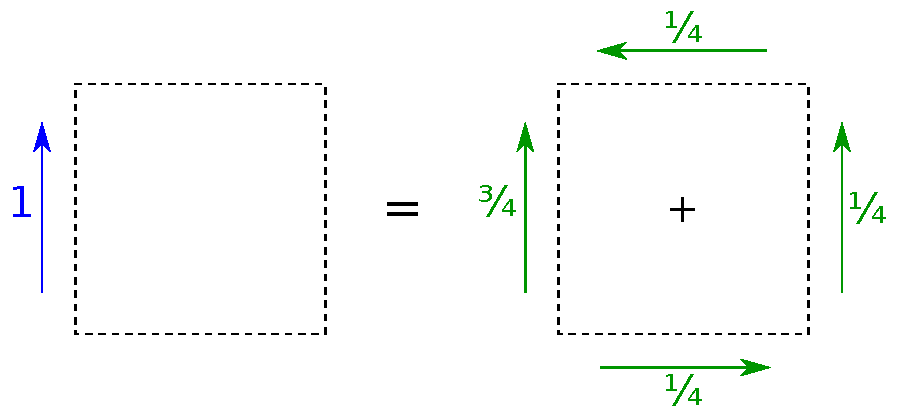
\includegraphics[width=0.6\linewidth]{3-ForceMap}%
  \caption[Weighting scheme to achieve zero torque]{Weighting scheme to achieve zero torque.  The left side is the force applied to a boundary and the right side contains the forces calculated from \autoref{eq:ShearForce}}%
  \label{fig:ForceMap}
\end{figure}

This mapping of shear velocities to shear forces is different from Stokes' viscous deformation law~\cite{Majumdar2005}\label{mark:Deformation}.  Both methods impose zero torque (i.e., conservation of rotational momentum without storage), but a discrete implementation of Stokes' viscous deformation law would do so at every boundary.  This is not necessary; the boundaries have zero thickness and thus zero moment.  However, there is a moment from the boundaries to the center of the control volumes.  Thus, the model imposes zero torque on each control volume as a whole.

If the normal bulk velocity is zero, the shear force equation reduces to
\begin{equation}
  \dot{mPhi}\sub{_D}[_para][ ]{_i} = \frac{2\s{Nu}\sub{_Phi}[_i]\s{A}[_i]}{\s{eta}\s{L}[_i]}\group{\s{phi}\sub{_para}[ ]{_i} - \s{phi}[_para]}
\end{equation}
If the velocity gradient is uniform ($\s{Nu}[_Phi] = 1$), translational momentum is not stored due to diffusion ($\dot{mPhi}\sub{_D}[_para][ ][_neg] = -\dot{mPhi}\sub{_D}[_para][ ][_pos] = \s{A}\s{J}$).  In that case, we can combine the negative- and positive-side equations as\label{mark:Couette}:
\begin{equation}
  \s{J} = \frac{\s{phi}\sub{_para}[ ][_neg] - \s{phi}\sub{_para}[ ][_pos]}{\s{eta}\s{L}}
\end{equation}
This maps directly to the actual shear stress if there is no shear force from the other two boundaries along the perimeter.  It is the first-order approximation to Newton's law of viscous shear, which describes Couette flow~\cite{Lienhard2006}. %[p. 281]

The shear force equation results in the expected pressure loss for fully-developed laminar pipe flow (i.e., Hagen-Poiseuille flow)\label{mark:Poiseuille}.  Suppose that material is flowing in the x direction with velocity~\s{phi} through a region with dimensions~\s{L}[_x], \s{L}[_y], and \s{L}[_z].  The bulk velocities in the y and z  directions are zero and the x-direction velocity is zero at the y and z boundaries (i.e., no slip).  According to \autoref{eq:ShearForce}, the total shear force on the y and z boundaries is
\begin{equation}
  \dot{mPhi}[_tot] = -\frac{4\s{Nu}[_Phi]\s{L}[_x]\s{phi}}{\s{eta}}\group{\frac{\s{L}[_z]}{\s{L}[_y]} + \frac{\s{L}[_y]}{\s{L}[_z]}}
\end{equation}
If the flow is fully developed, steady, and laminar, $\s{Nu}[_Phi] = 4$.  We may write the equation in terms of the hydraulic diameter ($\s{D} \equiv 4\s{A}/\s{P}$)~\cite{Incropera2002}, which is $2\s{L}[_y]\s{L}[_z]/(\s{L}[_y] + \s{L}[_z])$ in this case.  If there are no other forces the shear force must be balanced by the normal force ($\s{L}[_y]\s{L}[_z]\Delta\s{p} = \dot{mPhi}[_tot]$; see the conservation of translational momentum in \autoref{sec:BasicTranslationalBalance}).  With these assumptions and substitutions,
\begin{equation}
  \Delta\s{p} = \frac{64\s{L}[_x]\s{phi}}{\s{eta}\s{D}^2}\group{\frac{2}{2 + \frac{\s{L}[_y]}{\s{L}[_z]} + \frac{\s{L}[_z]}{\s{L}[_y]}} - 1}
\end{equation}
If we assume that the cross section is square ($\s{L}[_y] = \s{L}[_z]$), this reduces to
\begin{equation}
  \Delta\s{p} = -\frac{32\s{L}[_x]\s{phi}}{\s{eta}\s{D}^2}
\end{equation}
which is Poiseuille's law.  It can be derived by integrating a differential representation of the shear force equation (\ref{eq:ShearForce}) with a translational Nusselt number of one under the assumption of uniform pressure and a no-slip condition around a circular pipe~\cite{Cengel2006}.  This implies that the model should give the same result without the shear shape factor (i.e., $\s{Nu}[_Phi] = 1$) under a sufficiently fine level of discretization.  As mentioned previously, the shear shape factor is introduced to allow much coarser levels of discretization, and here it is set to four.

The model cannot directly describe turbulence\label{mark:Turbulence} because it assumes that the rotational momentum is zero.  This implies that eddies are not generated or are dissipated immediately upon generation.  A full description would require equations for the storage, exchange, and transport of rotational momentum.  Instead, correlations for turbulent flow are cast into the shear shape factor, which may vary with time and depend on the conditions.  This approach is consistent with the statement by Patankar~\cite{Patankar1980}: %[p.~15]
``From a computational viewpoint, a turbulent flow within this framework is equivalent to a laminar flow with a rather complicated prescription of viscosity.''  The only difference in this respect is that the present model has an adjustment factor (\s{Nu}[_Phi]) which is separate from the fluidity (or reciprocal of viscosity).

If rotational momentum were included, it is plausible that at a sufficiently fine level of discretization the model could describe turbulence.  In reality, shear force generates eddies that drive material towards alternating boundaries around the perimeter---normal to the direction of primary flow.  This effect would decrease the advection-adjusted length between the bulk velocity and a boundary (see \autoref{eq:ShearForce}) and increase the shear force for any velocity difference.  The criteria for the effect is that a sufficient amount of translational momentum is diverted from the direction of primary flow towards a boundary (e.g., by surface roughness).  It is a positive feedback mechanism; as more translational momentum is diverted towards the boundary due to shear force, more shear force is produced, until the translational momentum in the primary direction is sufficiently depleted.  Suppose we let \s{omega} be the diversion angle at the onset of the positive feedback.  Then, the P\'eclet number in the applicable shear force equation is
\begin{equation}
  \s{Pe} = \frac{\s{eta}\s{M}\s{phi}\sin\s{omega}}{\s{k}\s{A}}
\end{equation}
where \s{phi}~is the bulk velocity in the primary direction.  If we assume that the cross section is square, the hydraulic diameter is the length of a side ($\s{D} = \s{L} = \s{V}/\s{A}$).  If we also assume that the area factor is one ($\s{k} = 1$), then
\begin{equation}
  \s{Pe} = \s{mrho}\s{eta}\s{D}\s{phi}\sin\s{omega}
\end{equation}
The factor $\s{mrho}\s{eta}\s{D}\s{phi}$ is the Reynolds number; therefore
\begin{equation}
  \s{Pe} = \s{Re}\sin\s{omega}
\end{equation}
The discretization scheme becomes nearly saturated (as the upwind scheme) at roughly $\s{Pe} = 10$ (see \autoref{fig:AdvDiffRegion}) whereas turbulence begins at roughly 2300~\cite{Cengel2006}.  If we assume that turbulence corresponds to saturation of the discretization scheme, $\s{omega} \approx 0.25^\circ$.


\subsection{Thermal Advection and Conduction}
\label{sec:ThermalTransport}


As mentioned in \autoref{sec:BasicEnergyBalance}, the thermal transfer through an interface \s{i}~is divided into advective and diffusive parts:
\begin{equation}
  \label{eq:ThermalTransport}
  \dot{Q}[_i] = \dot{Q}\sub{_A}[_i] + \dot{Q}\sub{_D}[_i]
\end{equation}
This follows the form of \autoref{eq:Transport} where the transported quantity~(\s{X}) is heat~(\s{Q}).  This does not imply that heat is treated as a thermodynamic property; it only appears in a flow rate or a partial derivative, since it is process-dependent.  The advective term includes a component of enthalpy.  The diffusive part is thermal conduction.

As mentioned in \autoref{sec:BasicEnergyBalance}, thermal convection is the serial combination of thermal conduction and the advection of energy.  This is shown in \autoref{fig:ThermalConvection}.  The thermal conduction typically occurs between a solid and a fluid, which is an exchange process in the model.  However, we may assume that the thermal exchange occurs in a region of negligible thickness centered at the solid-fluid interface and that the fluid has the same temperature of the fluid there (i.e, no contact resistance).  Then, thermal convection is governed by two remaining processes in series: \begin{inparaenum}[(1)]\item thermal conduction between the fluid in the negligibly thin region and the fluid in a larger neighboring region and \item the advection through the larger region in the direction transverse to the boundary\end{inparaenum}.

\begin{figure}[htbp]
  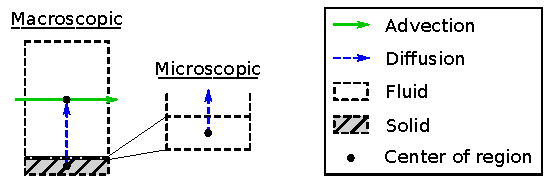
\includegraphics[width=0.65\linewidth]{3-ThermalConvection}%
  \caption{Thermal convection in the model}%
  \label{fig:ThermalConvection}
\end{figure}


\subsubsection{Advection}

Energy is advected according to the generalized advective transport equation (\ref{eq:AdvectiveTransport}) where the property $\partial\s{X}/\partial\s{N}$ is $\s{s}\s{T}$:
\begin{equation}
  \label{eq:ThermalAdvectiveTransport}
  \dot{Q}\sub{_A}[ ][_i] = \dot{N}[_i]\group{\s{s}\s{T}}[_i]
\end{equation}
The factor $(\s{s}\s{T})\sub{_i}$, combined with \s{g}[_i] of the material term, comprises the enthalpy associated with the material flow (as discussed in Sections~\ref{sec:BasicEnergyBalance} and \ref{sec:ThermalAdvectiveExchange}).  That factor is analogous to $\s{m}\s{phi}[_i]$ in the equations for translational advection (\ref{eq:NormalAdvection} and \ref{eq:TransverseAdvection}).  However, whereas the specific mass at the boundary is equal to the specific mass in the region, the specific entropy at the boundary is not generally equal to the specific entropy in the region ($\s{m}[_i] = \s{m}$, but $\s{s}[_i] \ne \s{s}$).  The temperature~(\s{T}) is the diffusion-driving property, like the velocity~(\s{phi}).


\subsubsection{Diffusion}

Like friction, thermal conduction or diffusion follows the form of the general transport equation (\ref{eq:DiffusiveTransport3}) with an adjustment factor (here, \s{Nu}[_Q]):
\begin{equation}
  \label{eq:ThermalDiffusiveTransport}
  \boxed{\s{theta}\dot{Q}[_i] = \frac{\s{Nu}[_Q]\s{k}[_i]\s{A}[_i]}{\s{L}[_i]}\group{\s{T}[_i] - \s{T}}\group{1 + e^{\mp\s{theta}\s{C}[_v]\s{phi}\sub{_perp}[_i]/2\s{k}[_i]\s{A}[_i]}}}
\end{equation}
The variable~\s{T}[_i] is the temperature at boundary~\s{i}, and $\dot{Q}[_i]$~is the rate of thermal conduction into the region through the boundary.  The temperature in the region~(\s{T}) may be considered known, since it is a state of the energy balance (\autoref{sec:BasicEnergyBalance}).

The thermal resistivity, \s{theta}, can be estimated from the generalized definition of resistivity (\autoref{eq:Resistivity}).
\begin{equation}
  \label{eq:ThermalResistivity}
  \boxed{\s{theta} = \frac{3\s{tau}}{\s{lambda}^2\s{rho}\s{c}[_v]}}
\end{equation}
where the partial derivative is taken at constant volume because the regions have fixed volume.  This equation matches the thermal conductivity given by Present~\cite{Present1958}, noting that thermal conductivity is the reciprocal of thermal resistivity~\cite{Incropera2002}.

The adjustment factor~\s{Nu}[_Q] is the traditional (thermal) Nusselt number\label{mark:Nusselt}.   It allows the thermal conduction equation to be used at relatively coarse levels of discretization.  It is the ratio of the average inward temperature gradient along the perimeter divided by the difference between the boundary temperature and the bulk temperature over the distance from the boundary to the center of the region:
\begin{equation}
  \label{eq:ThermalNusselt}
  \s{Nu}[_Q] \equiv \left.\diffp{\s{T}}{\s{x}}[_i]\middle/2\frac{\s{T}[_i] - \s{T}}{\s{L}[_x]}\right.
\end{equation}

At a macroscopic level, the temperature profile is not linear under thermal convection because the conducted heat is carried away by advection transverse to the boundary (\autoref{fig:ThermalConvection}).

Here, the Nusselt number is defined more generally than usual~\cite{Incropera2002}; it need not be used at a solid boundary.  Nonetheless, if it is applied to internal flow (fluid bounded by a solid conduit), its values correspond to the traditional ones.  For fully developed laminar flow in a circular pipe under a uniform boundary temperature, the Nusselt number is approximately 3.66.  With uniform heat flux, it is $48/11$ or approximately 4.36~\cite{Incropera2002}.



\subsubsection{Discussion}

If the bulk velocity (and advective current) is zero along the axis of transport and the area factor and Nusselt number are unity,\footnote{The latter could be due to the absence of advection or a fine level of discretization, either of which makes a linear temperature profile reasonable within the region.} then the thermal conduction equation (\ref{eq:ThermalDiffusiveTransport}) reduces to
\begin{equation}
  \s{theta}\dot{Q}[_i] = \frac{2\s{A}[_i]}{\s{L}[_i]}\group{\s{T}[_i] - \s{T}}
\end{equation}
If the temperature gradient is uniform, energy is not stored due to diffusion ($\dot{Q}[_neg] = -\dot{Q}[_pos] = \s{A}\s{J}$).  In that case, we can combine the negative- and positive-side equations as\label{mark:Fourier}
\begin{equation}
  \s{theta}\s{J} = \frac{\s{T}[_neg] - \s{T}[_pos]}{\s{L}}
\end{equation}
which is the first-order approximation to Fourier's law or the law of heat conduction~\cite{Incropera2002, Wesselingh2000}.%\cite[p.~53, 68]{Incropera2002}, \cite[p.~78]{Wesselingh2000}

The thermal Nusselt number is related to the heat transfer coefficient by
\begin{equation}
  \s{Nu}[_Q] = \frac{\s{h}\s{theta}\s{L}}{1 + e^{\mp\s{theta}\s{N}\s{c}[_v]\s{phi}[_perp]/2\s{k}\s{A}}}
\end{equation}
where $\s{L}/(1 + e^{\mp\s{theta}\s{N}\s{c}[_v]\s{phi}[_perp]/2\s{k}\s{A}})$ is the characteristic length.  Substituting this into the thermal conduction equation (\ref{eq:ThermalDiffusiveTransport}) under the assumption that the area factor is unity ($\s{k} = 1$)\label{mark:Newton},
\begin{equation}
  \dot{Q}[_i] = \s{h}\s{A}[_i]\group{\s{T}[_i] - \s{T}}
\end{equation}
which is Newton's law of cooling~\cite{Incropera2002}.


\section{Transport Properties}
\label{sec:TransportProperties}

\begin{contextbox}
  Highlights:
  \begin{itemize*}
    \item By default, the model estimates all diffusion properties based on the kinetic theory of gases, so they only depend on temperature, pressure, and the particle's mass and diameter.  It includes refinements where they are available and necessary.
  \end{itemize*}
\end{contextbox}

Due to the assumptions implicit in the diffusive transport equation (\ref{eq:DiffusiveTransport2}), the equations for the dynamic compressibility (\ref{eq:DynamicCompressibility}), material resistivity (\ref{eq:MaterialResistivity}), fluidity (\ref{eq:Fluidity}), and thermal resistivity (\ref{eq:ThermalResistivity}) are only taken to be estimates.  However, they are useful if more precise data is not available.  Those equations require the collision interval~(\s{tau}) and the mean free path (\s{lambda}), which were given for the exchange properties (\autoref{sec:ExchangeProperties}) under additional assumptions from the kinetic theory of gases.

The estimate of fluidity (\autoref{eq:Fluidity}) predicts that fluidity is independent of pressure or specific volume, which accurately matches observations~\cite{Present1958}.  However, the fluidity generally falls more rapidly with temperature than predicted~\cite{Present1958}.  Higher accuracy can be achieved for many common gases using the correlations by Svehla, McBride, and Gordon~\cite{Svehla1995, McBride1996}.  Those correlations have the following form:
\begin{equation}
  \boxed{\s{eta} = \s{b}_{\sep{\zeta}{1}}\ln{\s{T}} + \s{b}_{\sep{\zeta}{2}}/\s{T} + \s{b}_{\sep{\zeta}{3}}/\s{T}^2 + \s{b}_{\sep{\zeta}{4}}}%
  \glsadd{_zeta}\glsadd{_123}
\end{equation}
Higher accuracy can be achieved for thermal resistivity than \autoref{eq:ThermalResistivity} using correlations from the same source~\cite{Svehla1995, McBride1996}:
\begin{equation}
  \boxed{\s{theta} = \s{b}_{\sep{\theta}{1}}\ln{\s{T}} + \s{b}_{\sep{\theta}{2}}/\s{T} + \s{b}_{\sep{\theta}{3}}/\s{T}^2 + \s{b}_{\sep{\theta}{4}}}%
  \glsadd{_theta}\glsadd{_123}
\end{equation}


\section{Electrochemical Reactions}
\label{sec:Reaction}

% **concentration at rho0 at beginning far from interface, rises to interface (therefore opposite BC of current explanation, which has rho0 at gap); 10/25/13 p.~1 notes


\begin{contextbox}%
  Highlights:
  \begin{itemize*}
    \item The model uses the Butler-Volmer equation, which is derived in this section.
    \item The charge transfer coefficient appears explicitly in this derivation.
  \end{itemize*}
\end{contextbox}

The electrochemical reactions are described using the Butler-Volmer equation, but we will first derive it from the exchange equations of the model (\autoref{sec:Exchange}).  This derivation \begin{inparaenum}[(1)]\item relates the exchange current of the Butler-Volmer equation to the previously established parameters and \item indicates how to partition the reaction equations into submodels for the implementation in \autoref{chap:Implementation}\end{inparaenum}.


\subsection{Context}

The electrochemical reactions of a \nfirst{PEMFC} occur near the interface of the electrode or catalyst (e.g., platinum), which has free (conductance-band) electrons, and the electrolyte or ionomer, which has free protons.\footnote{ The term ``protons'' is used for simplicity, but to be more precise, the charge carriers are hydrogen nuclei.}  The interface is located in the catalyst layer as shown in \autoref{fig:ReactionContext}.  A thin layer of charge exists just inside the surface of the catalyst due to an excess or deficit of electrons there.  This charge attracts or repels positive ions from the neighboring ionomer.  We will assume that these ions are the protons themselves, but they may be a combination of other intermediaries of the anodic or cathodic half reaction (Equations \ref{eq:HOR} and \ref{eq:ORR}).  Over the \n{EDL}, the charge of the excess (or deficit) electrons balances the charge of the excess (or deficit) protons.  

The electrolytic side of the double layer consists of a surface layer and a diffuse layer.  The protons are the most concentrated or depleted (depending on attraction or repulsion) at the surface layer which is offset from the interface by a small gap (due to the nonzero particle size).  Over the diffuse layer, the concentration (or depletion) decays with distance from the interface much more slowly than for electrons.

\begin{figure}[htbp]
  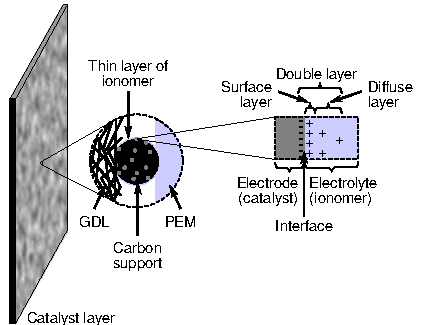
\includegraphics[width=0.65\linewidth]{3-ReactionContext}%
  \caption[Location of the electrochemical reaction]{The electrochemical reaction occurs in the double-layer region near the catalyst\slash{}ionomer interface (based on \cite[p. 74]{Larminie2003} and~\cite{Mazumder2003a})}%
  \label{fig:ReactionContext}
\end{figure}

The charge difference leads to an electric field which exerts forces on the ions, as shown in \autoref{fig:DoubleLayer}.  For simplicity, we will apply assumptions (such as sheet charge and others detailed below) that result in a uniform electric field and uniform drift velocities  over the gap.  Although the ions drift (i.e., are advected) across the gap, there is no net transport because advection cancels diffusion.  We assume that \begin{inparaenum}[(1)]\item the ions are reacted or stored as they pass the edge of the gap, \item the ionomer does not conduct electrons, and \item the catalyst does not conduct protons\end{inparaenum}.  

The reaction is driven by a difference in the concentrations of electrons between the free (conductance-band) and bound (e.g., as H relative to \s{H+}) forms at the edges of the gap.  Those concentrations are each a consequence of the constraint that advection cancels diffusion, beginning from the interface where we assume that the positive and negative ions exist at their bulk or charge-neutral concentration.\footnote{At this concentration, the charge of the ion is balanced by the charge of the substrate.  For example, the \s{e-} and \s{Pt+} would have the same concentration or \s{H+} and \s{SO3-} would have the same concentration.}  

Although the reaction coordinate is normal to the surface, the surface of the catalyst is oriented in all global directions.  Therefore, we will consider the reaction to be an exchange process.  The \n{EDL} is considered a distinct phase that only occupies part of the region.

\begin{figure}[htbp]
  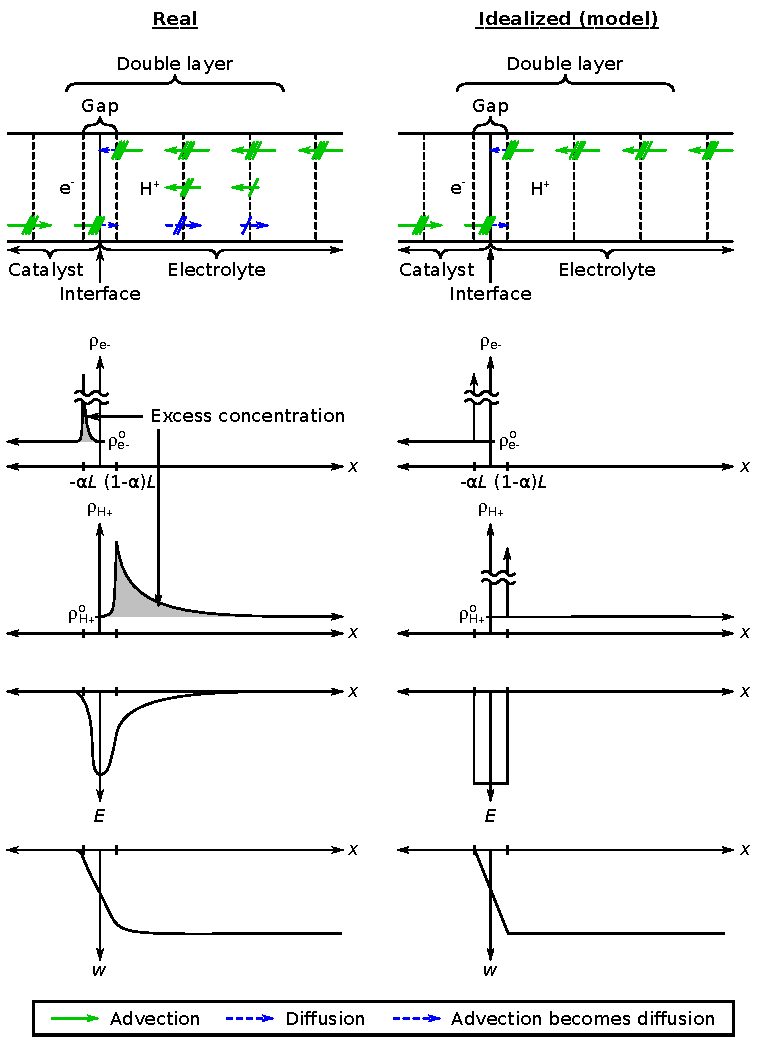
\includegraphics[width=\linewidth]{3-DoubleLayer}%
  \caption[Advection, diffusion, and properties along the reaction coordinate]{Advection, diffusion, concentration, electric field, and electrical potential along the reaction coordinate}%
  \label{fig:DoubleLayer}
\end{figure}

In summary, the reaction occurs within the double layer which contains a non-conducting gap surrounding the electrode\slash{}electrolyte interface.  There is potential for a charge difference across the double layer which produces an electric field that causes ions to drift across a non-conducting gap.  We assume that the ions drift to the edge of the gap and are stored or reacted there.  The reaction is a diffusive process driven by the difference in the concentration of electrons between the edges of the gap.  Within the gap, there is no net transport; drift must cancel diffusion.  This requirement establishes the concentrations at the edges of the gap, which yields the reaction rate.


\subsection{Equations}

We will assume that the limiting reaction is the combination or separation of the transported ions.  In the context of the \n{PEMFC}, this is
\begin{equation}
  \mathrm{H} \leftrightharpoons \s{e-} + \s{H+}
\end{equation}
We will return to this reaction below.  We will assume that the following reaction is in equilibrium and thus does not reduce the rate of the anodic reaction:
\begin{equation}
  \label{eq:AnChemical}
  \s{H2} \leftrightharpoons 2\timessep\mathrm{H}
\end{equation}
In the cathode, we will assume that the following reaction is in equilibrium:
\begin{equation}
  \label{eq:CaChemical}
  2\timessep\s{H2O} \leftrightharpoons 4\timessep\mathrm{H} + \s{O2}
\end{equation}
We will also assume that the water is vapor.  This assumption does not have a large effect because the evaporation\slash{}condensation process is rapid (see \autoref{sec:PhaseChange}).  At equilibrium, the stoichiometric sum of the specific Gibbs energies of the products and reactants is zero.  Therefore, from the previous two equations, the specific Gibbs energy of the hydrogen (H) is $\frac{1}{2}\s{g}[_H2]$ in the anode and $\frac{1}{2}\s{g}[_H2O] - \frac{1}{4}\s{g}[_O2]$ in the cathode.  

Like phase change, a reaction is driven by concentration differences.  The rate of the electrochemical reaction is the rate of diffusive exchange of electrons.  It follows from \autoref{eq:DiffusiveExchange2} for material ($\s{X} = \s{N}$, $\s{gamma} = \s{rho}$, $\partial\s{X}/\partial\s{gamma} = \s{V}$) that
\begin{equation}
  \label{eq:Reaction1a}
  \frac{8}{3\pi}\s{tau}[_e-]\timessep\dot{N}\sub{_D}[ ][_i][_e-] = \s{k}\sub{_i}[_e-]\s{V}[_e-]\group{\s{rho}[_i] - \s{rho}[_e-]}
\end{equation}
The conversion concentration, \s{rho}[_i], is the product of a rate constant and the concentrations of the other species (besides electrons) each raised to the power of their stoichiometric coefficients: $\s{b}\timessep\s{rho}[_H]/\s{rho}[_H+]$.  We will assume that state of the hydrogen (H) varies isothermally and as an ideal gas up to the specific Gibbs energy of conversion (\s{g}[_H]).  Therefore,
\begin{equation}
  \label{eq:Reaction2a}
  \frac{8}{3\pi}\s{tau}[_e-]\timessep\dot{N}\sub{_D}[ ][_i][_e-] = \s{k}\sub{_i}[_e-]\s{V}[_e-]\group{\frac{\s{b}\timessep\s{p}[^o]}{\s{rho}[_H+]\s{T}}e^{\s{g}[_H]/\s{T}} - \s{rho}[_e-]}
\end{equation}
where \s{p}[^o]~is the reference pressure of the ideal gas.  

The concentrations of the electrons and the protons are evaluated at the edges of the gap.  We can determine those concentrations from the transport model under two assumptions: \begin{inparaenum}[(1)]\item at the interface, the concentrations are equal to the bulk concentrations and \item across the gap, there is no net transfer of ions\end{inparaenum}.  The second assumption implies that advection cancels diffusion.  If two adjacent regions have the same resistance to diffusion of the ion, it follows from Equations \ref{eq:DiffusiveTransportTwoRegion} and \ref{eq:MaterialTransport} that
\begin{equation}
  0 = \s{A}\s{phi}\s{rho} + \frac{\s{rho}_1 - \s{rho}_2}{\s{R}}
  \glsadd{_123}
\end{equation}
where \s{phi}~is the velocity at a boundary and \s{rho}~is the excess concentration there.  The resistance~(\s{R}) is $\s{zeta}\s{L}/\s{k}\s{A}$ (see \autoref{eq:Resistance1}, where the resistivity \s{r}~is the material resistivity \s{zeta}), but we will assume that the area factor (\s{k}) is one. Therefore,
\begin{equation}
  0 = \s{zeta}\s{phi}\s{rho} + \frac{\s{rho}_1 - \s{rho}_2}{\s{L}}
  \glsadd{_123}
\end{equation}
We can write this as a differential equation (taking the limit as $\s{L} \to 0$):
\begin{equation}
  \s{zeta}\s{phi}\s{rho}\mathrm{d}\s{x} = \mathrm{d}\s{rho}
\end{equation}
From the interface to the edge of the gap, the solution for the first ion is
\begin{equation}
  \s{rho}_1 = \s{rho}_1\sup{^o}\timessep e^{-\s{alpha}\s{zeta}_1\s{phi}_1\s{L}}
\end{equation}
where \s{alpha}~is the fraction of the length of the gap (\s{L}) that exists on the side of the first ion.  It is commonly called the charge transfer coefficient~\cite{Bockris1973}.  The factor of $\s{zeta}\s{phi}\s{L}$ in the argument of the exponential is the P\'eclet number of diffusive material transport (\autoref{sec:MaterialDiffusion}). The variable $\s{rho}_1\sup{^o}$ is the bulk or charge-neutral concentration of the ion.  The solution for the second ion is
\begin{equation}
  \s{rho}_2 = \s{rho}_2\sup{^o}\timessep e^{\group{1 - \s{alpha}}\timessep\s{zeta}_2\s{phi}_2\s{L}}
\end{equation}
The velocities in the previous two equations can be determined from the momentum balance (\autoref{eq:TranslationalBalanceIntensive}) under the assumption that the velocity is at steady state and there is no gravitational acceleration, surface force, or force due to advective exchange.
\begin{equation}
  \s{Z}\s{E} = \dot{mPhi}\sub{_D}[_E]
\end{equation}
We will assume that the electric field is uniform across the gap ($\s{E} = \s{w}/\s{L}$).  The drag force ($\dot{mPhi}\sub{_D}[_E]$) is $\s{N}\s{phi}/\s{mu}$ due to \autoref{eq:TranslationalDiffusiveExchange} under the assumption that the drag is with a stationary interface (zero mediation velocity) and the adjustment factor is one.  The mobility (\s{mu}) is $1/\s{zeta}\s{T}$ according to the Einstein relation (\autoref{sec:EinsteinRelation}).  Therefore,
\begin{equation}
  \s{phi} = \frac{\s{z}\s{E}}{\s{zeta}\s{T}}
\end{equation}
With this, the concentrations of the two ions are
\begin{equation}
  \s{rho}_1 = \s{rho}_1\sup{^o}\timessep e^{-\s{alpha}\timessep \s{z}_1\s{w}/\s{T}}
\end{equation}
and
\begin{equation}
  \s{rho}_2 = \s{rho}_2\sup{^o}\timessep e^{\group{1 - \s{alpha}}\timessep\s{z}_2\s{w}/\s{T}}
\end{equation}
Therefore, the reaction rate (from \autoref{eq:Reaction2a}) is
\begin{equation}
  \label{eq:Reaction3a}
  \frac{8}{3\pi}\s{tau}[_e-]\timessep\dot{N}\sub{_D}[ ][_i][_e-] = \s{k}\sub{_i}[_e-]\s{V}[_e-]\group{\frac{\s{b}\timessep\s{p}[^o]}{\s{rho}[_H+][^o]\s{T}}e^{\Group{\s{g}[_H] \pm \group{\s{alpha} - 1}\timessep\s{w}}/\s{T}} - \s{rho}[_e-][^o]e^{\pm\s{alpha}\s{w}/\s{T}}}
\end{equation}
where $\pm$ is positive if the electrons are on the first side (and protons on the second) or negative 
if the protons are on the first side (and electrons on the second).  

As written, the previous equation may lead to numerical issues because the arguments of the exponentials may be large at open circuit (on the order of 40 in the cathode of a \n{PEMFC}).  To help, we will use a relative electrical potential---the activation overpotential---instead of the double-layer potential.  The overpotential is relative to the equilibrium potential:
\begin{equation}
  \boxed{\s{w}[^prime] = \s{w} - \s{w}[_eq]}
\end{equation}
At the equilibrium potential (\s{w}[_eq]), there is no net reaction ($\dot{N}\sub{_D}[ ][_i][_e-] = 0$).  From \autoref{eq:Reaction3a},
\begin{equation}
  \pm\s{w}[_eq] = \s{g}[_H] + \s{T}\ln\group{\frac{\s{b}\timessep\s{p}[^o]}{\s{rho}[_e-][^o]\s{rho}[_H+][^o]\s{T}}}
\end{equation}
By default, the logarithmic term is removed in the model, which implies that $\s{b} = \s{rho}[_e-][^o]\s{rho}[_H+][^o]\s{T}/\s{p}[^o]$.  
\begin{equation}
  \boxed{\pm\s{w}[_eq] = \s{g}[_H]}
\end{equation}
In terms of the overpotential, \autoref{eq:Reaction3a} is
\begin{equation}
  \label{eq:Reaction4a}
  \frac{8}{3\pi}\s{tau}[_e-]\timessep\dot{N}\sub{_D}[ ][_i][_e-] = \s{k}\sub{_i}[_e-]\s{V}[_e-]\group{\frac{\s{b}\timessep\s{p}[^o]}{\s{rho}[_H+][^o]\s{T}}}^{\s{alpha}}\group{\s{rho}[_e-][^o]}^{1 - \s{alpha}}\timessep e^{\s{g}[_H]/\s{T}}\Group{e^{\pm\group{\s{alpha} - 1}\timessep\s{w}[^prime]/\s{T}} - e^{\pm\s{alpha}\s{w}[^prime]/\s{T}}}
\end{equation}
or
\begin{equation}
  \label{eq:Reaction}
  \boxed{\dot{N}\sub{_D}[ ][_i][_e-] = \s{I}[^o]\Group{e^{\pm\group{\s{alpha} - 1}\timessep\s{w}[^prime]/\s{T}} - e^{\pm\s{alpha}\s{w}[^prime]/\s{T}}}}
\end{equation}
where the exchange current, \s{I}[^o], is defined below.  Due to this equation, heat is generated at the rate of $\mp\s{w}[^prime]\dot{N}\sub{_D}[ ][_i][_e-]$ in the gap.  We can write the reaction rate in terms of electrical current from the first side towards the second ($\s{z}\s{I} = \mp\dot{N}\sub{_D}[ ][_i][_e-]$):\label{mark:BV}
\begin{equation}
  \label{eq:Reaction6a}
  \s{z}\s{I} = \pm\s{I}[^o]\Group{e^{\pm\s{alpha}\s{w}[^prime]/\s{T}} - e^{\pm\group{\s{alpha} - 1}\timessep\s{w}[^prime]/\s{T}}}
\end{equation}
This is the Butler-Volmer equation~\cite{Bockris2000, Prentice1991, Newman1991}, 
%\cite[p.~111]{Prentice1991}, \cite[pp.~337, 521]{Newman1991}
where $\s{z}\s{I}$ is the electrical current.  Again, $\pm$ is positive if the electrons are on the first side or negative if the protons are on the first side.  

The exchange current, \s{I}[^o], is
\begin{equation}
  \s{I}[^o] = \frac{3\pi}{8}\frac{\s{k}\sub{_i}[_e-]}{\s{tau}[_e-]}\s{V}[_e-]\group{\frac{\s{b}\timessep\s{p}[^o]}{\s{rho}[_H+][^o]\s{T}}}^{\s{alpha}}\group{\s{rho}[_e-][^o]}^{1 - \s{alpha}}\timessep e^{\s{g}[_H]/\s{T}}
\end{equation}
Since it is assumed that $\s{b} = \s{rho}[_e-][^o]\s{rho}[_H+][^o]\s{T}/\s{p}[^o]$,
\begin{equation}
  \boxed{\s{I}[^o] = \frac{3\pi}{8}\frac{\s{k}\sub{_i}[_e-]}{\s{tau}[_e-]}\group{\s{V}[_e-]\s{rho}[_e-][^o]}\timessep e^{\s{g}[_H]/\s{T}}}
\end{equation}
The factor of $\s{V}[_e-]\s{rho}[_e-][^o]$ is the number of electrons that would exist in the gap if they existed at the bulk concentration over the entire gap (either as free \s{e-} or as H in excess of~\s{H+}).  In practice, the exchange current (or exchange current density) is an empirical, tunable parameter or correlation (e.g.,~\cite{Sivertsen2005}).  

The electrical potential across the gap, \s{w}, depends on the charge in the \n{EDL}, its distribution, and the permittivity of the \n{EDL}.  We have assumed that the charges are uniformly distributed over parallel planes (i.e., infinitely thin sheet charges) and the electric field is uniform over the gap.  Assuming also that the electrical capacitance is constant, the following dynamic relationship is introduced:
\begin{equation}
  \label{eq:ElectricalCap}
  \boxed{\s{z}\s{I} = \frac{\s{epsilon}\s{A}}{\s{L}}\diffp{\s{w}}{\s{t}}}
\end{equation}
where \s{epsilon}~is the electrical permittivity over the gap and $\s{epsilon}\s{A}/\s{L}$ is the electrical capacitance.  It is important to note that the capacitance is associated with the electrical potential (\s{w}), not the overpotential (\s{w}[^prime]).  The total current is the sum of the storage current from this equation and the reaction current from \autoref{eq:Reaction6a}.

The force applied to ion~\s{i} at the edge of the gap is 
\begin{equation}
  \boxed{\dot{mPhi}[_D] = \mp\s{z}[_i]\s{rho}[_i][^o]\s{A}\s{w}}
\end{equation}
This force that yields the drift velocity within the gap.  The electrical capacitor is the only component of the entire model (this chapter) that does not conserve translational momentum.  The forces on the positive and negative ions will not be equal and opposite if the ions have different bulk concentrations (\s{rho}[_i][^o]). 
 


\clearpage % **Is this necessary to prevent heading at bottom of page?
\section{Detailed Conservation Equations}
\label{sec:DetailedConservation}

\begin{contextbox}
  Highlights:
  \begin{itemize*}
    \item The conservation equations explicitly and exactly account for all flows due to exchange and transport.  Convergence does not depend on the mesh size as in \n{CFD} methods~\cite{Celia1990} because the flow rates are shared between adjacent regions.  As long as the simulation runs, conservation is guaranteed within the simulation tolerance.  This allows the discretization to be coarse; only several regions are necessary to model a \n{PEMFC}.
    \item The model includes all of the effects in the compressible Navier-Stokes equations---convective acceleration, unsteady acceleration, pressure gradients, shear stresses, and body force.
    \item The energy conservation equation includes heat generation due to all of the modeled diffusive or irreversible effects.
    \item Thermal advection is essential to phase change and reactions; it captures the enthalpy of formation.  Translational advection may be excluded in the model of a typical \n{PEMFC} since the surface layer is stationary.  However, it is included for completeness and may be important in other devices.
  \end{itemize*}
\end{contextbox}
\vspace{0.7\baselineskip}

% \begin{figure}[!htb]
%   \newcommand{\vgap}{\vphantom{Energy}}
%   \centering
%   \begin{tikzpicture}
%     [level distance=1.5cm]
%     \Tree[.FC\\Model
%            [.{Conservation\vgap}
%               [.\node[xshift=-0.5mm]{Material\vgap}; ]
%               [.\node[xshift=-0.5mm]{Linear\\Momentum}; ]
%               [.\node[xshift=-0.5mm]{Energy\vgap}; ] ] ]
%   \end{tikzpicture}
%   \caption{Conserved quantities in the fuel cell model}
% \end{figure}

% Methods that do not explicitly conserve mass:
%   localized adjoint methods (LAMs) including Eulerian-Lagrangian localized adjoint method (ELLAM)~\cite{Celia1990}

The basic conservation equations were given in \autoref{sec:BasicConservation}.  Here they are expanded with the terms developed in the exchange, transport, and reaction sections (\ref{sec:Exchange}, \ref{sec:Transport}, and \ref{sec:Reaction}) and further analyzed.

The analysis includes the consideration of time constants.  The time constants of the various processes are given by
\begin{equation}
  \label{eq:TimeConstant}
  \s{tau} = \group{\diffp{\s{X}}{\s{gamma}}}\group{\diffp{\s{gamma}}{\dot{X}}}
\end{equation}
where \s{X}~is a transferred quantity and \s{gamma}~is an intensive property that drives its diffusive exchange or transport.  Thus, each time constant is the product of a generalized capacitance ($\partial\s{X}/\partial\s{gamma}$) and a generalized resistance ($\partial\s{gamma}/\partial\dot{X}$)


\subsection{Material}
\label{sec:MaterialBalance}

The intake terms of the basic material conservation equation (\autoref{eq:MaterialBalance}) can be divided into exchange and transport.
\begin{equation}
  \newcommand{\vgap}{\vphantom{\sum_{i \in \text{E}}\dot{N}\sub{_D}[_i]}}
  \label{eq:MaterialBalance2}%
  \underbrace{\vgap\diffp{\s{N}}{\s{t}}}_\text{storage} =  \,\, \underbrace{\vgap\sum_{i \in \text{E}}\dot{N}\sub{_D}[_i]}_\text{exchange} \,\,\,\, + \,\, \underbrace{\vgap\sum_{i \in \text{T}}\big(\underbrace{\vgap\dot{N}\sub{_D}[_i]}_\text{diffusion} \pm \underbrace{\vgap\s{phi}\sub{_perp}[_i]\s{rho}[_i]\s{A}[_i]}_\text{advection}\big)}_\text{transport}
  \glsadd{_E}
  \glsadd{_Tr}
\end{equation}
where the transport current has been expanded into advective and diffusive parts using Equations \ref{eq:MaterialTransport} and \ref{eq:MaterialAdvection}.  As noted in \autoref{sec:Exchange}, there is no advective exchange of material.  The sum in the exchange group is over all phase change and reaction processes in which the configuration participates.  The sum in the transport group is over the boundaries.

If the phase in which the configuration exists has constant volume, the material conservation equation may be written as
\begin{equation}
  \s{V}\diffp{\s{rho}}{\s{t}} = \sum_{i \in \text{E}}\dot{N}\sub{_D}[_i] + \sum_{i \in \text{T}}\big(\dot{N}\sub{_D}[_i] \pm \s{phi}\sub{_perp}[_i]\s{rho}[_i]\s{A}[_i]\big)
  \glsadd{_E}
  \glsadd{_Tr}
\end{equation}
The advective currents ($\s{phi}\sub{_perp}[_i]\s{rho}[_i]$) may be written as \s{J}[_i].  Dividing this by volume, expanding the transport terms, and assuming that there is no diffusive transport\label{mark:Continuity},
\begin{equation}
  \diffp{\s{rho}}{\s{t}} = \frac{\sum_{i \in \text{E}}\dot{N}\sub{_D}[_i]}{\s{V}} + \frac{\s{J}\sub{_x}[_neg] - \s{J}\sub{_x}[_pos]}{\s{L}[_x]} + \frac{\s{J}\sub{_y}[_neg] - \s{J}\sub{_y}[_pos]}{\s{L}[_y]} + \frac{\s{J}\sub{_z}[_neg] - \s{J}\sub{_z}[_pos]}{\s{L}[_z]}
\end{equation}
which is the first-order spatial approximation of the continuity equation~\cite{Incropera2002, Fluent6.3}. %\cite[p.~323]{Incropera2002}, \cite[p.~635]{Fluent6.3}
Nevertheless, a first-order approximation is sufficient because the model's formulation allows the temporal integrator to guarantee convergence within a prescribed simulation tolerance.  The fluxes or currents are represented by variables that are explicitly shared between adjacent regions; therefore, the mass lost by one region is exactly the mass gained by another.  This is the essence of the continuity equation.


\subsubsection{Time Constants}
\label{sec:MaterialTime}


Based on \autoref{eq:TimeConstant}, the time constant due to material exchange is
\begin{equation}
  \s{tau}\sub{_N}[_E] = \s{V}\diffp{\s{rho}}{\dot{N}}
\end{equation}
This implies that the associated time constants are zero for isochoric species.  For a gas undergoing isothermal phase change, the time constant is
\begin{equation}
  \s{tau}\sub{_N}[_E] = \s{tau}[^prime]\frac{\s{N}[_g]\s{T}[_c]}{\s{N}[_c]}\diffp{\s{p}[_g]}{\s{rho}[_g]}[_T]\exp\group{\frac{\s{g}[_c] - \s{g}[_g]}{\s{T}[_c]}}
\end{equation}
based on Equations \ref{eq:PhaseChange} and \ref{eq:GibbsFunction}, where \s{tau}[^prime]~is the effective collision interval (\autoref{eq:EffectiveCollisionInterval}).  The subscript~g indicates the gas phase and the subscript~c indicates the condensed phase.  The partial derivative $\diffp{\s{p}}{\s{rho}}$ is $-\s{v}^2\diffp{\s{p}}{\s{v}}$, which can be determined using \autoref{eq:VirialLeiden1} or \ref{eq:VirialBerlin1}.  If the gas is ideal, then
\begin{equation}
  \s{tau}\sub{_N}[_E] = \s{tau}[^prime]\frac{\s{N}[_g]\s{T}[_c]}{\s{N}[_c]\s{T}[_g]}\exp\group{\frac{\s{g}[_c] - \s{g}[_g]}{\s{T}[_c]}}
\end{equation}
For a species~\s{i} participating in an isothermal electrochemical reaction, the time constant is
\begin{equation}
  \s{tau}\sub{_N}[_E] = \frac{2\s{N}[_i]\s{T}}{\s{J}[^o]\s{A}\group{e^{\s{Pe}/2} + e^{-\s{Pe}/2}}}\diffp{\s{rho}[_i]}{\s{p}[_i]}[_T]
\end{equation}
based on Equations \ref{eq:Reaction} and \ref{eq:GibbsFunction}, assuming the exchange current density (\s{J}[^o]) is constant and the charge transfer coefficient~(\s{alpha}) is one half.  Again, the partial derivative $\partial\s{p}/\partial\s{rho}$ can be determined using \autoref{eq:VirialBerlin1}.  If the species is an ideal gas, then
\begin{equation}
  \s{tau}\sub{_N}[_E] = \frac{2\s{N}[_i]}{\s{J}[^o]\s{A}\group{e^{\s{Pe}/2} + e^{-\s{Pe}/2}}}
\end{equation}
For an electrical species,
\begin{equation}
  \s{tau}\sub{_N}[_E] = \frac{2\s{T}\s{epsilon}}{\s{J}[^o]\s{L}\group{e^{\s{Pe}/2} + e^{-\s{Pe}/2}}}
\end{equation}
assuming that the only storage of the charge carrier is in the electrical capacitor with permittivity~\s{epsilon} described by \autoref{eq:ElectricalCap}.


Using the material diffusion equation (\ref{eq:MaterialDiffusion}), the time constant due to material transport through a boundary at constant extensive volume is
\begin{equation}
  \boxed{\s{tau}\sub{_N}[_Tr] = \frac{\s{zeta}\s{V}\s{L}}{\s{k}\s{A}\group{1 + e^{\mp\s{zeta}\s{V}\s{phi}[_perp]/2\s{k}\s{A}}}}}
\end{equation}
where the volume~(\s{V}) is the volume of the phase.  However, the area~(\s{A}) is the cross-sectional area of the region along the axis of transport and \s{L}~is the length of the same.  If the bulk material flow is towards a boundary, the associated time constant is smaller because the effective transport length is smaller.  The limiting cases are $\s{tau}\sub{_N}[_T] = 0$ (direct coupling) for infinite dimensionless material flow rate towards a boundary, $\s{tau}\sub{_N}[_Tr] = \s{zeta}\s{L}^2/2\s{k}$ for pure diffusion, and $\s{tau}\sub{_N}[_Tr] = \s{zeta}\s{L}^2/\s{k}$ for infinite flow away from the boundary.


The previous equation and similar ones below are boxed because they are implemented in the model (\autoref{chap:Implementation}).  However, they are nonessential;  they are only used to characterize the behavior due to other properties.



\subsection{Translational Momentum}
\label{sec:TranslationalBalance}

The conservation of translational momentum (\autoref{eq:TranslationalBalance}) can be written in terms of an intensive derivative by expanding the transient term using the chain rule and incorporating the conservation of material (\autoref{eq:MaterialBalance}):
\begin{equation}
  \label{eq:TranslationalBalanceIntensive}
  \boxed{\s{M}\diffp{\s{phi}}{\s{t}} + \s{M}\s{a} + \s{Z}\s{E} + \s{A}\Delta\s{p}[_i] = \sum\Group{\s{m}\group{\s{phi}[_i] - \s{phi}}\dot{N}[_i] + \dot{mPhi}\sub{_D}[_i]}}
\end{equation}
For each transport interaction, the current consists of advective and diffusive parts according to \autoref{eq:MaterialTransport}.  For each advective exchange interaction, the current (\dot{N}[_i]) is only the diffusive current ($\dot{N}\sub{_D}[_i]$), since there is no advective material exchange.

The previous equation can be expanded by separating the exchange and transport terms and applying \autoref{eq:TranslationalAdvectiveExchange} for advective exchange.
\begin{multline}%
  \label{eq:TranslationalBalanceIntensive2}
  \s{M}\diffp{\s{phi}}{\s{t}} + \s{M}\s{a} + \s{Z}\s{E} + \s{A}\Delta\s{p}[_i] = \sum_{i \in \text{exchange}}\Group{\s{m}
  \GROUP{\begin{aligned}
    \s{phi}[_i] - \s{phi}& \quad\text{if $\dot{N}[_i] > 0$,}\\
    0& \quad\text{if $\dot{N}[_i] \leq 0$}
  \end{aligned}}\dot{N}[_i] + \dot{mPhi}\sub{_D}[_i]} \\
  + \sum_{i \in \text{transport}}\Group{\s{m}\group{\s{phi}[_i] - \s{phi}}\dot{N}[_i] + \dot{mPhi}\sub{_D}[_i]}
\end{multline}
where the first sum is over the exchange interfaces and the second sum is over the transport interfaces.  As mentioned in \autoref{sec:Exchange}, the exchange interactions are either \begin{inparaenum}[(1)]\item advective, whereby the diffusion term ($\dot{mPhi}\sub{_D}[_i]$) is zero or \item diffusive, whereby the current \dot{N}[_i] is zero\end{inparaenum}.

This form of the translational momentum balance more clearly shows the conditions that cause the material to accelerate in the region from a Eulerian perspective.\label{mark:Eulerian}\footnote{\label{note:EulerianLagrangian}Acceleration from a Eulerian perspective (i.e., convective acceleration) indicates that the mean velocity of particles within the region increases over time.  This is different from acceleration from a Lagrangian perspective---the acceleration of a particle or fluid parcel.}   The advective term on the second line of \autoref{eq:TranslationalBalanceIntensive2} relates to the time-independent term of the material derivative of translational momentum~\cite{Bird2002}, the convective acceleration term in the Navier-Stokes equations, and as discussed in \autoref{sec:NormalAdvection}, the dynamic pressure.   Phase change and reaction have effects if the configuration is produced at a conversion velocity that is different from the present velocity.  The conversion velocity depends on the velocities of the configurations being consumed (see \autoref{sec:TranslationalExchange}).  If the configuration itself is consumed, the phase change or reaction has no effect since the configuration is consumed at its own velocity.  If material enters through a boundary ($\dot{N}[_i] > 0$) with a velocity greater than the velocity of the material within the region ($\s{phi}[_i] > \s{phi}$), the velocity of the material in the region will tend to increase.  The velocity is also affected by other configurations in the same region and the same configuration in other regions through the diffusion terms ($\dot{mPhi}\sub{_D}[_i]$).  Finally, the body forces ($\s{M}\s{a}$ and $\s{Z}\s{E}$) and the thermodynamic force ($\s{A}\Delta\s{p}[_i]$) affect the velocity.

The thermodynamic pressure at each boundary is a function of the local temperature and concentration ($\s{p}[_i] = \s{p}(\s{T}[_i]\text{, }\s{rho}[_i])$).  If the configuration is incompressible, then the thermodynamic pressure is the reference pressure (\s{p}[^o]) and the thermodynamic contribution is zero.  The pressure commonly used in the literature (often denoted by~\s{p} as well) is the sum of the thermodynamic pressure (\s{p}) and the nonequilibrium pressure ($\pm\dot{mPhi}[_i]/\s{A}$) over all the species in a phase.

\autoref{eq:TranslationalBalanceIntensive2} is closely related to the Navier-Stokes equation\label{mark:NS}.  If we combine the momentum balances of all the configurations in the region, the exchange terms disappear:
\begin{equation}
  \s{M}\diffp{\s{phi}}{\s{t}} + \s{M}\s{a} + \s{Z}\s{E} + \s{A}\Delta\s{p}[_i] = \sum_{i \in \text{transport}}\Group{\s{m}\group{\s{phi}[_i] - \s{phi}}\dot{N}[_i] + \dot{mPhi}\sub{_D}[_i]}
\end{equation}
We will assume that concentration is uniform.  This implies that there is no material diffusion and each boundary current is directly related to the bulk velocity in the normal direction (e.g., $\dot{N}\sub{_x}[_neg]/\s{V} = -\dot{N}\sub{_x}[_pos]/\s{V} = \s{rho}\s{phi}[_x]/\s{L}[_x]$). Dividing the equation by volume and applying it to the x~axis,
\begin{multline}%
  \s{mrho}\group{\diffp{\s{phi}[_x]}{\s{t}} + \frac{\s{phi}\sub{_x}[_pos][_x] - \s{phi}\sub{_x}[_neg][_x]}{\s{L}[_x]}\s{phi}[_x] + \frac{\s{phi}\sub{_y}[_pos][_x] - \s{phi}\sub{_y}[_neg][_x]}{\s{L}[_y]}\s{phi}[_y] + \frac{\s{phi}\sub{_z}[_pos][_x] - \s{phi}\sub{_z}[_neg][_x]}{\s{L}[_z]}\s{phi}[_z]} + \s{rho}\group{\s{m}\s{a}[_x] + \s{z}\s{E}[_x]} + \frac{\s{p}\sub{_x}[ ][_pos] - \s{p}\sub{_x}[ ][_neg]}{\s{L}[_x]}\\
  = \frac{\dot{mPhi}\sub{_D}[_x][_neg][_x] + \dot{mPhi}\sub{_D}[_x][_pos][_x] + \dot{mPhi}\sub{_D}[_y][_neg][_x] + \dot{mPhi}\sub{_D}[_y][_pos][_x] + \dot{mPhi}\sub{_D}[_z][_neg][_x] + \dot{mPhi}\sub{_D}[_z][_pos][_x]}{\s{V}}
\end{multline}
where $\s{phi}\sub{_x}[_neg][_x]$ is the x~component of velocity at the negative-x boundary, $\s{phi}\sub{_y}[_pos][_x]$ is the x~component of velocity at the positive-y boundary, et cetera.  The same convention applies to the subscripts in the shear force terms.  We can expand the viscous forces using \autoref{eq:NormalDiffusion} for the normal axes and \autoref{eq:ShearForce} for the transverse axes, assuming the P\'eclet numbers are negligible and the area factors and translational Nusselt numbers are unity.  We will also rewrite the volumic body terms ($\s{rho}(\s{m}\s{a} + \s{z}\s{E})$) as $-\s{f}/\s{V}$:
\begin{multline}%
  \s{mrho}\group{\diffp{\s{phi}[_x]}{\s{t}} + \frac{\s{phi}\sub{_x}[_pos][_x] - \s{phi}\sub{_x}[_neg][_x]}{\s{L}[_x]}\s{phi}[_x] + \frac{\s{phi}\sub{_y}[_pos][_x] - \s{phi}\sub{_y}[_neg][_x]}{\s{L}[_y]}\s{phi}[_y] + \frac{\s{phi}\sub{_z}[_pos][_x] - \s{phi}\sub{_z}[_neg][_x]}{\s{L}[_z]}\s{phi}[_z]} + \frac{\s{p}\sub{_x}[ ][_pos] - \s{p}\sub{_x}[ ][_neg]}{\s{L}[_x]}\\
  = \frac{\s{f}[_x]}{\s{V}} + 2\group{\frac{\s{phi}\sub{_x}[_neg][_x] + \s{phi}\sub{_x}[_pos][_x] - 2\s{phi}[_x]}{\s{beta}\s{L}[_x]^2} + \frac{\s{phi}\sub{_y}[_neg][_x] + \s{phi}\sub{_y}[_pos][_x] - 2\s{phi}[_x]}{\s{eta}\s{L}[_y]^2} + \frac{\s{phi}\sub{_z}[_neg][_x] + \s{phi}\sub{_z}[_pos][_x] - 2\s{phi}[_x]}{\s{eta}\s{L}[_z]^2}}
\end{multline}
If we assume that the dynamic compressibility~(\s{beta}) and the fluidity~(\s{eta}) are both equal to the reciprocal of dynamic viscosity~(\s{mu}), this is
\begin{multline}%
  \s{mrho}\group{\diffp{\s{phi}[_x]}{\s{t}} + \frac{\s{phi}\sub{_x}[_pos][_x] - \s{phi}\sub{_x}[_neg][_x]}{\s{L}[_x]}\s{phi}[_x] + \frac{\s{phi}\sub{_y}[_pos][_x] - \s{phi}\sub{_y}[_neg][_x]}{\s{L}[_y]}\s{phi}[_y] + \frac{\s{phi}\sub{_z}[_pos][_x] - \s{phi}\sub{_z}[_neg][_x]}{\s{L}[_z]}\s{phi}[_z]} + \frac{\s{p}\sub{_x}[ ][_pos] - \s{p}\sub{_x}[ ][_neg]}{\s{L}[_x]}\\
  = \frac{\s{f}[_x]}{\s{V}} + 2\s{mu}\group{\frac{\s{phi}\sub{_x}[_neg][_x] + \s{phi}\sub{_x}[_pos][_x] - 2\s{phi}[_x]}{\s{L}[_x]^2} + \frac{\s{phi}\sub{_y}[_neg][_x] + \s{phi}\sub{_y}[_pos][_x] - 2\s{phi}[_x]}{\s{L}[_y]^2} + \frac{\s{phi}\sub{_z}[_neg][_x] + \s{phi}\sub{_z}[_pos][_x] - 2\s{phi}[_x]}{\s{L}[_z]^2}}
\end{multline}
which is the first-order approximation to the x-axis Navier-Stokes equation for an incompressible, Newtonian, and homogeneous fluid~\cite{Majumdar2005, Deen1998, Newman1991}.  The first of the two groups on the left side is the material derivative of translational momentum~\cite{Bird2002}. %[p.~83].
The variable~\s{f} is force rather than volumic force.  %The first-order approximation is sufficient because the velocities and forces are represented by variables that are explicitly shared between adjacent regions.  Therefore, the translational momentum lost by one region is exactly the translational momentum gained by another.
Similar equations apply to the other axes.

Although the model characterizes compressible flow, it is not equivalent to the Navier-Stokes equations for compressible flow.  As discussed in \autoref{sec:TransverseTransport}, the shear force equations are mapped differently than by Stokes' viscous deformation law.  In addition, the Navier-Stokes equations consider the effects of compressibility using a volumetric divergence term ($\boldsymbol{\nabla}\cdot\boldsymbol{\phi}$), whereas the model does so with the normal force equation (\ref{eq:NormalDiffusion}).


\subsubsection{Time Constants}
\label{sec:TranslationalTime}

Based on Equations \ref{eq:TimeConstant} and \ref{eq:TranslationalDiffusiveExchange}, the time constant due to diffusive translational exchange is
\begin{equation}
  \boxed{\s{tau}\sub{_Phi}[_E] = \frac{\s{m}\s{mu}}{\s{k}}}
\end{equation}
This time constant is directly related to the mean collision interval~(\s{tau}) under the assumptions of kinetic theory (\autoref{sec:Exchange}).  By applying \autoref{eq:Mobility},
\begin{equation}
  \s{tau}\sub{_Phi}[_E] = \frac{8}{3\pi\s{k}}\s{tau}
\end{equation}
which is typically small (assuming $\s{k} = 1$)---on the order of \SI{20}{ns} for oxygen in air (see \autoref{sec:ExchangeProperties}).  Thus, it is appropriate to assume that the velocities of different species are equal within a phase unless they are driven by significant opposing forces.  Based on Equations \ref{eq:TimeConstant} and \ref{eq:NormalDiffusion}, the time constant due to dynamic compression is
\begin{equation}
  \boxed{\s{tau}\sub{_Phi}[_perp] = \frac{\s{beta}\s{M}\s{L}}{2\s{k}\s{A}}}
\end{equation}
assuming that the configuration fills the entire region ($\s{V} = \s{V}[_tot]$).  Based on Equations \ref{eq:TimeConstant} and \ref{eq:ShearForce}, the time constant due to shear force is
\begin{equation}
  \boxed{\s{tau}\sub{_Phi}[_para] = \frac{\s{eta}\s{M}\s{L}}{\s{Nu}[_Phi]\s{k}\s{A}\group{1 + e^{\mp\s{eta}\s{M}\s{phi}[_perp]/2\s{k}\s{A}}}}}
\end{equation}
This time constant depends on the normal velocity at the boundary (\s{phi}[_perp]), just as the material transport time constant does (\autoref{sec:MaterialTime}).


\subsection{Energy}
\label{sec:EnergyBalance}

The energy conservation equation (\ref{eq:EnergyBalance}) can be written in terms of intensive derivatives by expanding the transient terms and incorporating the material conservation equation (\ref{eq:MaterialBalance2}):
\begin{equation}
  \label{eq:EnergyBalanceIntensive}
  \boxed{\s{M}\s{phi}\diffp{\s{phi}}{\s{t}} + \s{N}\s{T}\diffp{\s{s}}{\s{t}} = \sum\Group{\group{\s{g}[_i] + \group{\s{T}\s{s}}[_i] - \s{h} + \s{m}\frac{\s{phi}[_i]^2 - \s{phi}^2}{2}}\dot{N}[_i] + \s{phi}[_i]\dot{mPhi}\sub{_D}[_i] + \dot{Q}\sub{_D}[_i]}}
\end{equation}
The Gibbs energy relation (\autoref{eq:g}) has been applied to reduce $\s{g} + \s{T}\s{s}$ but not $\s{g}[_i] + \group{\s{T}\s{s}}[_i]$ yet (for reasons that will be apparent).  We can eliminate the local acceleration term (at the expense of adding other terms) by subtracting the translational momentum balance (\autoref{eq:TranslationalBalanceIntensive}) times velocity~(\s{phi}):

\begin{multline}
  \label{eq:EnergyBalanceIntensive2}
  \s{N}\s{T}\diffp{\s{s}}{\s{t}} = \s{phi}\group{\s{M}\s{a} + \s{Z}\s{E} + \s{A}\Delta\s{p}[_i]} \\
  + \sum\Group{\group{\s{g}[_i] + \group{\s{T}\s{s}}[_i] - \s{h} + \frac{\s{m}}{2}\group{\s{phi}[_i] - \s{phi}}^2}\dot{N}[_i] + \group{\s{phi}[_i] - \s{phi}}\dot{mPhi}\sub{_D}[_i] + \dot{Q}\sub{_D}[_i]}
\end{multline}
Now the interface velocities (\s{phi}[_i]) only appear relative to the velocity in the region~(\s{phi}).  The new term on the right side, $\s{phi}\group{\s{M}\s{a} + \s{Z}\s{E} + \s{A}\Delta\s{p}[_i]}$, is the opposite (negative) of the rate of energy necessary to overcome the effect of the static forces on the control volume.  The advective and diffusive terms (second line) must contribute energy at this rate in order to maintain a steady-state value of specific entropy.

At transport interfaces (boundaries), the material and thermal contributions are considered together; therefore, $\s{g}[_i] + \group{\s{T}\s{s}}[_i]$ reduces to \s{h}[_i].  At exchange interfaces (transitions) where the configuration is a source (reactant), $(\s{T}\s{s})\sub{_i} = \s{T}\s{s}$ and $\s{phi}[_i] = \s{phi}$ due to Equations \ref{eq:TranslationalAdvectiveExchange} and \ref{eq:ThermalAdvectiveExchange}; therefore, $\s{g}[_i] + \group{\s{T}\s{s}}[_i] - \s{h} + \frac{\s{m}}{2}(\s{phi}[_i] - \s{phi})^2$ reduces to $\s{g}[_i] - \s{g}$.  As a result, we can write the energy conservation equation as

\begin{multline}
  \label{eq:EnergyBalanceIntensive3}
  \s{N}\s{T}\diffp{\s{s}}{\s{t}} = \s{phi}\group{\s{M}\s{a} + \s{Z}\s{E} + \s{A}\Delta\s{p}[_i]} \\
  \begin{aligned}
    + \sum_{\s{i} \in \text{exchange}}\Group{\GROUP{\begin{aligned}
      \s{g}[_i] + \group{\s{T}\s{s}}[_i] - \s{h} + \frac{\s{m}}{2}\group{\s{phi}[_i] - \s{phi}}^2& \quad\text{if $\dot{N}[_i] > 0$,}\\
      \s{g}[_i] - \s{g} &\quad\text{if $\dot{N}[_i] \leq 0$}
    \end{aligned}}\cdot\dot{N}[_i] + \group{\s{phi}[_i] - \s{phi}}\dot{mPhi}\sub{_D}[_i] + \dot{Q}\sub{_D}[_i]} \\
    + \sum_{\s{i} \in \text{transport}}\Group{\group{\s{h}[_i] - \s{h} + \frac{\s{m}}{2}\group{\s{phi}[_i] - \s{phi}}^2}\dot{N}[_i] + \group{\s{phi}[_i] - \s{phi}}\dot{mPhi}\sub{_D}[_i] + \dot{Q}\sub{_D}[_i]}
  \end{aligned}
\end{multline}
where the first sum is over the exchange interfaces and the second sum is over the transport interfaces.  The factor $(\s{s}\s{T})\sub{_i}$ in the exchange sum (for products) is the thermal conversion property, which depends on the reactants (sources) according to \autoref{eq:ThermalConversionProperty}.  The relation between the specific Gibbs energy at the interface (\s{g}[_i]) and the specific Gibbs energy of the configuration~(\s{g}) depends on the phase and the rate of the reaction or phase change process.  The rate equation for phase change is implemented within the condensed phase (see \autoref{sec:PhaseChange}); therefore, the specific Gibbs energy at the interface of the condensed phase is subject to \autoref{eq:PhaseChange}.  The rate equation for electrochemical reactions is implemented in the phase where electrons are the majority charge carrier (see \autoref{sec:Reaction}), and the activation overpotential occurs there.  For the other phases, including gas, the specific Gibbs energy at the interface is equal to the specific Gibbs energy of the configuration ($\s{g}[_i] = \s{g}$).  Those phases do not incur any of the irreversible heat of the process, regardless of the direction of the process.


We can use the previous equation to identify the factors that affect the temperature of the configuration.  The temperature will increase if, and only if, the specific entropy increases.\footnote{Specific entropy and temperature are related in general by $\s{T}\mathrm{d}\s{s} = \s{c}\timessep\mathrm{d}\s{T}$, where \s{T} and~\s{c} are both positive.  Based on \autoref{eq:s}, $\s{T}\mathrm{d}\s{s}$ is $\s{c}[_p][^o]\mathrm{d}\s{T}$ if the configuration has no thermal expansion and $\s{c}[_p][^o]\mathrm{d}\s{T} - \s{v}\mathrm{d}\s{p}$ if it is an ideal gas.}  So far, we have seen that the specific entropy of the configuration will increase if \begin{inparaenum}[(1)]\item material or translational momentum enters through an interface where the velocity is greater than the velocity of the configuration ($\s{phi}[_i] > \s{phi}$) or \item the configuration drives a reaction or phase change due to a difference in specific Gibbs energy\end{inparaenum}.  In general, the specific entropy will increase if material enters with a specific enthalpy (\s{h}[_i]) greater than that of the configuration (\s{h}).  The specific entropy will also increase if heat is conducted into the configuration ($\dot{Q}\sub{D}[_i] > 0$).

Some of these processes are reversible and some are irreversible.  It is possible to identify the irreversible ones by evaluating the net change of extensive entropy in two interacting configurations.  However, the transfer mechanisms of the model are clearly delineated as advective and diffusive, and the diffusive processes are irreversible.  The advective processes are irreversible only to the extent that they are coupled with diffusion.  In \autoref{sec:Transport}, we called this process irreversible advection.  In the model, it only occurs in transport---not in exchange.


The energy conservation equation is related to the heat equation\label{mark:Heat}.  The heat equation is typically written for an entire region, so we add \autoref{eq:EnergyBalanceIntensive3} over all the configurations in the region.  This eliminates the exchange terms.  We also assume that there is no material advection or diffusion.  Therefore,
\begin{equation}
  \s{N}\s{T}\diffp{\s{s}}{\s{t}} = \s{phi}\group{\s{M}\s{a} + \s{Z}\s{E} + \s{A}\Delta\s{p}[_i]} + \sum_{\s{i} \in \text{transport}}\Group{\group{\s{phi}[_i] - \s{phi}}\dot{mPhi}\sub{_D}[_i] + \dot{Q}\sub{_D}[_i]}
\end{equation}
We will assume that the pressure is constant; therefore, $\s{T}\partial\s{s} = \s{c}[_p]\partial\s{T}$.  Heat is generated by viscous dissipation to the extent that $\sum\group{\s{phi}[_i] - \s{phi}}\dot{mPhi}\sub{_D}[_i]$ exceeds $-\s{phi}\group{\s{M}\s{a} + \s{Z}\s{E} + \s{A}\Delta\s{p}[_i]}$, the rate of energy necessary to overcome the effect of the static forces on the control volume.  Therefore,
\begin{equation}
  \s{N}\s{c}[_p]\diffp{\s{T}}{\s{t}} = \dot{Q}[_gen] + \sum\dot{Q}\sub{_D}[_Tr][_i]
\end{equation}
where \dot{Q}[_gen] is the rate of heat generation and $\sum\dot{Q}\sub{_D}[_Tr][_i]$ is the total rate of thermal conduction into the region.  We can evaluate the thermal conduction using \autoref{eq:ThermalDiffusiveTransport} under the assumption that the Nusselt number (\s{Nu}[_Q]) and the area factor~(\s{k}) are both one.  The P\'eclet numbers are all zero due to the previous assumption that there is no material advection.  After dividing by volume,
\begin{equation}
  \s{rho}\s{c}[_p]\diffp{\s{T}}{\s{t}} = \frac{2}{\s{theta}}\Group{\frac{\s{T}\sub{_x}[_neg] + \s{T}\sub{_x}[_pos] - 2\s{T}}{\s{L}_x^2} + \frac{\s{T}\sub{_y}[_neg] + \s{T}\sub{_y}[_pos] - 2\s{T}}{\s{L}_y^2} + \frac{\s{T}\sub{_z}[_neg] + \s{T}\sub{_z}[_pos] - 2\s{T}}{\s{L}_z^2}} + \frac{\dot{Q}[_gen]}{\s{V}}
\end{equation}
This is the first-order spatial approximation to the heat diffusion equation assuming uniform thermal resistivity~\cite{Incropera2002}. %[p.~63]
The variable $\s{T}\sub{_x}[_neg]$~is the temperature at the negative-x boundary, $\s{T}\sub{_y}[_pos]$~is the temperature at the positive-y boundary, et cetera.


\subsubsection{Time Constants}
\label{sec:ThermalTime}

Based on Equations \ref{eq:TimeConstant} and \ref{eq:ThermalDiffusiveExchange}, the time constant due to diffusive thermal exchange is
\begin{equation}
  \boxed{\s{tau}\sub{_Q}[_E] = \frac{\s{c}[_p]\s{nu}}{\s{k}}}
\end{equation}
where the specific heat capacity is isobaric (\s{c}[_p]) because the pressures of the configurations are assumed to be at equilibrium (see \autoref{sec:AmagatsLaw}).  This time constant is directly related to the mean collision interval~(\s{tau}) under the assumptions of kinetic theory (\autoref{sec:Exchange}).  By applying \autoref{eq:ThermalIndependity},
\begin{equation}
  \s{tau}\sub{_Q}[_E] = \frac{8}{3\pi\s{k}}\s{tau}
\end{equation}
which is typically small (assuming $\s{k} = 1$)---on the order of \SI{20}{ns} for oxygen in air (see \autoref{sec:ExchangeProperties}).  Thus, it is appropriate to assume that the temperatures of different species are equal within a phase unless there is significant heat generation due to a reaction, for example.  Based on Equations \ref{eq:TimeConstant} and \ref{eq:ThermalDiffusiveTransport}, the time constant due to diffusive thermal transport is
\begin{equation}
  \label{eq:TimeConstantThermalTransport}
  \boxed{\s{tau}\sub{_Q}[ ][_Tr] = \frac{\s{theta}\s{C}[_v]\s{L}}{\s{Nu}[_Q]\s{k}\s{A}\group{1 + e^{\mp\s{theta}\s{C}[_v]\s{phi}[_perp]/2\s{k}\s{A}}}}}
\end{equation}
This time constant depends on the normal velocity at the boundary (\s{phi}[_perp]), just as the material transport time constant does (\autoref{sec:MaterialTime}).



\section{Summary}

This chapter established a multi-component, multi-phase model of advective and diffusive transport and exchange with dynamic conservation of material, momentum, and energy.  The model supports electrochemical reactions and phase change between a condensed or absorbed phase and a gas.  The model is spatially distributed in three dimensions, yet it has been discretized for \np{DAE} with exact conservation at every boundary.  The next chapter will review the implementation of the model in the Modelica language.


% Use single-spacing in the context boxes again.
\renewenvironment{contextbox}
{\vspace{-0.7em}
   \begin{framed}
    \begin{singlespaced}
   \setlength\parindent{0pt}}
{  \end{singlespaced}
 \end{framed}}


  \chapter{Implementation of the Model}
  \label{chap:Implementation}
  %%%%%%%%%%%%%%%%%%%%%%%%%%%%%%%%%%%
%% Setup
%%%%%%%%%%%%%%%%%%%%%%%%%%%%%%%%%%%

\glsresetall
\glsunset{H2O}

% Create a row in a table that references the documentation.
\DeclareDocumentCommand\docrow{mom}{% mandatory (m), optional (o), mandatory (m)
  \ifthenelse{\equal{#2}{\NoValue}}{%
    \hspace{0.9em}\labelitemi\hspace{1.0\itemsep}\ref{#1} & \hyperref[#1]{\modelica{#3}} \\
  }{%
    \hspace{0.9em}\labelitemi\hspace{1.0\itemsep}\ref{#1}--\ref{#2} & \modelica{#3} \\
  }
}

% Trim and frame GUI images.
\DeclareDocumentCommand\gui{om}{% optional (o), mandatory (m)
  \ifthenelse{\equal{#1}{\NoValue}}{%
    \fbox{\lwincludegraphics[clip, trim=6 6 6 23.5]{#2}}
  }{%
    \fbox{\lwincludegraphics[clip, trim=6 6 6 23.5, #1]{#2}}
  }%
}%

% Border for GUI images
\setlength\fboxsep{0pt}
\setlength\fboxrule{0.5pt}

%%%%%%%%%%%%%%%%%%%%%%%%%%%%%%%%%%%
%% Content
%%%%%%%%%%%%%%%%%%%%%%%%%%%%%%%%%%%
 
% \begin{singlespaced}
%   \epigraph{``The idea that terminal variables can be divided into efforts and flows appears to be a deep---but unfortunately largely unexplored---physical principle, corroborated by many examples.''}{Jan Willems~\cite{Willems2007}}
% \end{singlespaced}

This chapter describes how the model is implemented in the Modelica language~\cite{Modelica3.3}.  It serves primarily as a summary for \autoref{chap:Doc}, which contains documentation generated from the source code.  The documentation contains auto-generated tables, diagrams, and code listings.  It also contains discussions and other details such as lists of assumptions which have been manually written and embedded using Modelica's annotations.  That information is only referenced here to avoid redundancy.

The introduction below merely sets the context to describe the model library.  For an introduction to the Modelica language, see~\cite{Tiller2002} or~\cite{ModelicaTutorial1.4}.


\section{Introduction}

The models are special object-oriented classes in the Modelica language.  The model library also uses other classes such as connectors, blocks, functions, records, packages, types.  The classes are encapsulated and organized hierarchically via inheritance and instantiation.  Encapsulation or abstraction hides details about the implementation, leaving only the meaningful characteristics accessible from outside the class~\cite{Pyster2012}. %[p. 91]
Inheritance creates models or other classes by extending or adding to more general and basic classes.  It helps to organize the library and reduce the amount of duplication in the code.  Instantiation allows classes to be built by assembling working copies of lower-level classes.  This is consistent with the physical hierarchy of the fuel cell (e.g., a cell is an assembly of layers).  \autoref{fig:ModelHierarchy2} shows that the model is created by instantiating species into phases, phases into subregions, subregions into regions such as a fuel cell layer, and regions into assemblies such as a fuel cell.  By convention, the names of classes begin with an uppercase letter and their instances start with a lowercase letter.  Subclasses and sub-instances are accessed via dot notation (e.g., \modelica{Class.Subclass1.Subclass2}).


\begin{figure}[htbp]
  \newcommand{\I}[1]{\fbox{\includegraphics[height=2cm]{#1}}}
  \newcommand{\arrow}{\vbox to 1.95cm {\vfil
    \hbox{\LARGE $\rightarrow$}
    \vfil}}
  \I{4-SpeciesI}~\arrow~\I{4-PhaseI}~\arrow~\I{4-SubregionI}~\arrow~\fbox{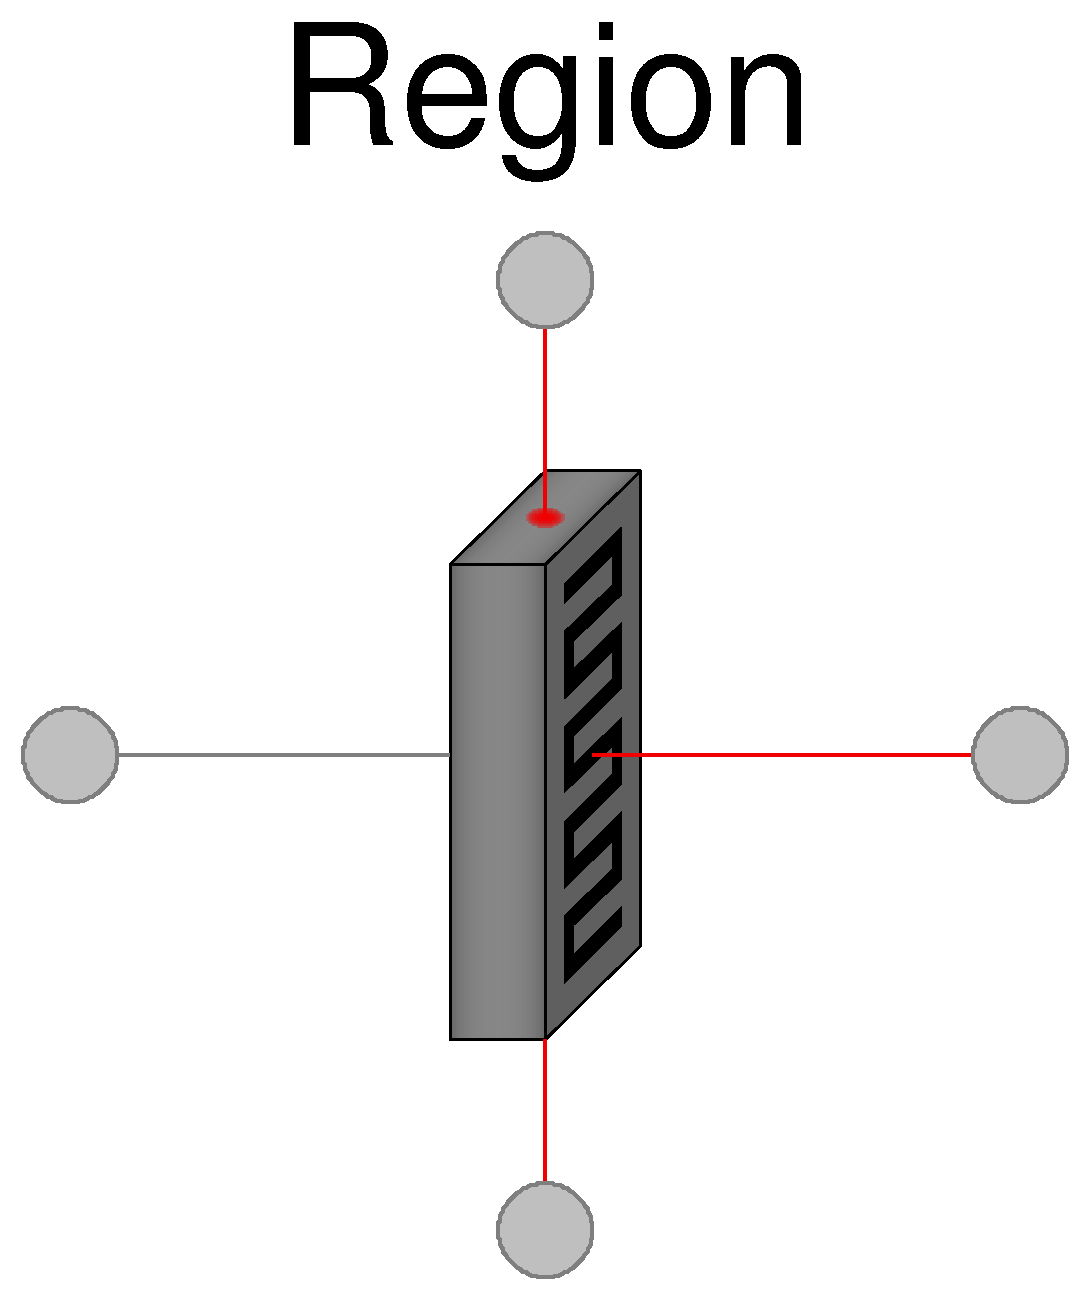
\includegraphics[height=2.4cm]{4-RegionI}}~\arrow~\I{4-AssemblyI}%
  \caption{Levels of instantiation in the model library (duplicate of \autoref{fig:ModelHierarchy})}%
  \label{fig:ModelHierarchy2}%
\end{figure}


Each model is a system with possible subsystems.  The physical connectors (i.e., connectors containing efforts and flows, to be discussed later) of the model represent its boundaries.  The boundaries may be geometric (e.g., the positive boundary along the x axis; see \autoref{fig:Flow3DLabel}) or conceptual (e.g., between two species within a phase).

The equations of a model may be represented graphically or textually.  Usually, the higher-level models are graphical whereas the lower-level ones are textual.  In the diagrams, lines between physical connectors (\autoref{sec:Connectors}) comprise nodes which are subject to the generalized Kirchhoff circuit laws (e.g., efforts are equal and flows sum to zero).  The icons represent instances of classes.

The term \emph{\n{state}} should be clearly defined because it has two different (but related) meanings in mathematical modeling and thermodynamics.  In the context of modeling and Modelica\glsadd{state-model}, a state is a scalar time-varying variable of which a derivative is taken.\footnote{These may or may not be the same variables which are wrapped by the \modelica{der()} operator since the Modelica translator is usually free to choose appropriate states.  Also, those variables may be algebraically coupled, in which case the translator must perform index reduction.}  The states of a model are necessary and sufficient to determine the values of all other variables of the model at a given time.  In the context of thermodynamics\glsadd{state-thermo}, a state is the condition of a system.  It encompasses a set of properties with cardinality equal to the degrees of freedom of the system in the sense of Gibbs' phase rule~\cite{Moran2004, Bejan2006}.  Since the fuel cell models involve thermodynamics, both meanings may be used.  A thermodynamic state is represented by a set of model states---generally one for each mode of energy storage (e.g., pressure and temperature).

The remaining sections describe the model library from low to high level.  The first sections describe supporting classes such as types (\autoref{sec:Quantities}), constants (\autoref{sec:Units}), records and functions (\autoref{sec:Characteristics}), and connectors (\autoref{sec:Connectors}).  The models begin with the subregions in \autoref{sec:Subregions} and continue up to the test models in \autoref{sec:TestStand}.


\section{Quantities}
\label{sec:Quantities}

\begin{contextbox}
  Related section of the documentation:
  \vspace{0.5\baselineskip}

  \renewcommand{\arraystretch}{1.5}
  \begin{tabular}{ll}
    \docrow{sec:FCSys_Quantities}{FCSys.Quantities}
  \end{tabular}
\end{contextbox}

Quantities are types used to represent physical values in the model library.  Each quantity has a dimension which is specified in terms of angle (A), length (L), mass (M), particle number (N), and time (T).  Quantities may also have default display units and minimum or maximum values.

Instances of quantities are variables.  The names of the variables match those in \autoref{chap:Fundamentals} with the exceptions that \begin{inparaenum}[(1)]\item Greek letters are spelled in English and \item subscripts begin with an underscore\end{inparaenum}.  Usually, extensive properties are uppercase and intensive properties are lowercase.

The quantities package is described further in the documentation (\autoref{sec:FCSys_Quantities}).  Throughout the rest of this chapter and the appendix, the \modelica{Quantities} package may be abbreviated as \modelica{Q} (e.g., \modelica{Q.Length}).


\section{Units}
\label{sec:Units}

\begin{contextbox}
  Related sections of the documentation:
  \vspace{0.5\baselineskip}

  \renewcommand{\arraystretch}{1.5}
  \begin{tabular}{ll}
    \docrow{sec:FCSys_Units}{FCSys.Units}
    \docrow{sec:FCSys_Units_Bases}[sec:FCSys_Units_Bases_Base]{FCSys.Units.*}
  \end{tabular}
\end{contextbox}

The \modelica{Units} package is described in \autoref{sec:FCSys_Units} with updated information from the related paper~\cite{Davies2012ModelicaUnits}.  In summary, the approach is based on the concept that a quantity is the product of a number and a unit~\cite{BIPM2006}.  The variables in the library represent quantities,  in contrast to the usual approach where variables represent numbers or quantities expressed in a unit (where ``expressed in'' means divided by).  When a variable is given a quantity in the library, it is expressed literally as the product of a number and a unit or group of units.  This provides convenience and flexibility in entering values (e.g., \modelica{101325*Pa} or \modelica{1*atm}).  When the variable is expressed in a unit, it is divided by that unit (e.g., \modelica{p/kPa}).

The units package begins by giving values to certain fundamental, physical, and measurable constants (the speed of light in vacuum and the Rydberg, Josephson, von Klitzing, Faraday, and gas constants).\footnote{The radian and candela are also given values to complete the basis.  As discussed, the radian must be one due to the definition in~\cite{BIPM2006}.}  The values are arbitrary except that they can be used to additionally scale the floating point variables.  The units are then determined by the accepted values of the constants (e.g., $c = \SI{299792458}{m/s}$ from~\cite{NIST2010}).  The constants have independent dimensions such that they are sufficient to determine the values of all other units.  Approximately 90 constants, units, and prefixes are defined.  All are instances of quantities (as defined in \autoref{sec:Quantities}).

As noted in the beginning of \autoref{chap:Fundamentals}, the model equations are written in a system of units where the Faraday and gas are normalized to one.  Literally, this means that $\SI{1}{mol} = \SI{96485.3365}{C}$.  The coulomb is used as a number of particles just as the mole, but the charge number is applied appropriately when describing an electric field or an electric current.  Since the Faraday and gas constants are both normalized, temperature is equivalent to thermal voltage (e.g., $\SI{300}{K} \approx \SI{25.85}{mV}$).  This also implies that the Boltzmann constant is normalized to \s{q}, the particle number representing a single particle.  These normalizations simplify the equations and make it straightforward to model electrons and protons like other species (albeit with nonzero charge number).

During the implementation, it was discovered that the document which establishes the International System of Units (SI)\glsunset{SI}~\cite{BIPM2006} may inconsistently define and use angles.  Table~3 in that document states that the radian (rad) is defined by $\si{rad} \equiv 1$ and the hertz (Hz) is defined by $\si{Hz} \equiv \si{s^{-1}}$.  However, we commonly consider the hertz to be a measure of ``cycles per second'' or $\si{Hz} = \si{cyc}/\si{s}$, where the cycle (cyc) is defined by $\si{cyc} \equiv \SI{2\pi}{rad}$ in trigonometry.  Since $\si{rad} \equiv 1$, it follows that $\si{cyc} = 2\pi$.  This implies that $\si{Hz} = 2\pi/\si{s}$, which is not consistent with the \n{SI} definition ($\si{Hz} \equiv \si{s^{-1}}$).

The discrepancy could be resolved by defining angle as an explicit dimension (like length and time) with units that include the radian, cycle, and degree.  Those units are related (e.g., $\si{cyc} \equiv \SI{2\pi}{rad}$) but none should be given a fixed value.  That is the approach in the \modelica{Units} package, but it is limited by the fixed \n{SI} definition of $\si{rad} \equiv 1$.  The approach also resolves issues such as the seemingly identical units of energy (\si{J}) and torque (\si{N.m})~\cite{McNish1957} by using angle in the units for torque (e.g., $\si{J/rad}$).  In this sense, torque is a unit of energy per swept angle.  Traditionally, we express the angle in radians but exclude it (since it is one) and then consider torque to be the product of force and radius.

Throughout the rest of this chapter and the appendix, the \modelica{Units} package may be abbreviated as \modelica{U}.  For example, \modelica{U.m} is the unit meter.


\section{Characteristics}
\label{sec:Characteristics}

\begin{contextbox}
  Related sections of the documentation:
  \vspace{0.5\baselineskip}

  \renewcommand{\arraystretch}{1.5}
  \begin{tabular}{ll}
    \docrow{sec:FCSys_Characteristics_BaseClasses_Characteristic}[sec:FCSys_Characteristics_O2_Gas]{FCSys.Characteristics.*}
  \end{tabular}
\end{contextbox}

The \modelica{Characteristics} package contains data and functions to correlate physical properties of materials.  The data and functions are contained within a package for each chemical species.  All of the correlated and derived thermodynamic properties (Sections~\ref{sec:CorrelatedThermo} and \ref{sec:DerivedThermo}) and diffusion properties (Sections~\ref{sec:Exchange} and \ref{sec:Transport}) are coded from the descriptions in the previous chapter.  The characteristics are suitable for real and ideal gases, compressible and incompressible fluids, and solids.  \autoref{tab:FCSys_Characteristics_BaseClasses_Characteristic-contents} lists the data and functions.

The Modelica media package (\modelica{Modelica.Media}~\cite{ModelicaSL3.2}) is not used besides its data.  There are four reasons.  First, it would be necessary to rewrite the variable declarations since the model library uses a different approach to physical units (see the previous section).  Second, many of the functions would need to be wrapped to convert the properties for the equations established in \autoref{chap:Fundamentals}.  This would introduce overhead in terms of both computation and software maintenance.  Third, some properties are not available in \modelica{Modelica.Media}.  Other properties and correlations are present but are not needed.  Finally, the models are factored differently in the present library.  The \modelica{Characteristics} package does not include any models or time-varying variables (in the \modelica{Species} model instead---next section), unlike \modelica{Modelica.Media}.

The virial coefficients (\s{p}-\s{v}-\s{T} relation) for the Leiden (volume-explicit) form are encoded in a matrix (\s{b}[_v]).  The power of $\s{p}/\s{T}$ increases by row and the power of~\s{T} increases by column, beginning with the powers set by~\s{n}[_v] (a 2-tuple).  The matrix for the Berlin (pressure-explicit) form (\s{b}[_p]) is computed automatically but is currently limited to the fourth virial coefficient.  It can be expanded to an arbitrary order with results from a \n{CDF} file included with the library.  The Leiden is directly prescribed instead of the Berlin form so that the specific volume of incompressible species can be entered.  The resulting polynomials are encoded in all the property functions using the nested form (e.g., $f(x) = ((\ldots + a_\text{-1-n})/x + a_\text{-n})/x + a_\text{1-n} + x\cdot(a_\text{2-n} + x\cdot(a_\text{3-n} + \ldots))$) for computational efficiency.

The isobaric specific heat capacity-temperature relation also allows arbitrary polynomial order, starting from an arbitrary power.  This makes it possible to prescribe constant or temperature-dependent specific heat capacity as needed.  The relation is independent of pressure, but following the approach by Dymond et al.~\cite{Dymond2002}, the rows of the coefficients matrix (\s{b}[_c]) cover different temperature ranges.  An arbitrary number of rows can be included, which is an improvement over \modelica{Modelica.Media}.

A base characteristics record is extended for each of the chemical species required for the fuel cell model---\n{C+}, negatively charged Nafion sulfonate (\s{C19HF37O5S-}, abbreviated as \s{SO3-}), \n{e-}, \n{H+}, \n{H2}, water vapor, liquid water, water absorbed in the ionomer, \n{N2}, and \n{O2}.  Where available, virial and heat capacity coefficients are included respectively from~\cite{Dymond2002} and~\cite{McBride2002} (directly or via \modelica{Modelica.Media}).  These representations are later simplified (e.g., to ideal gas and constant specific heat capacity) as appropriate.   The polynomial coefficients for the specific heat capacity of water in the ionomer and the associated integration constants for enthalpy and entropy are set so that the hydration of the ionomer matches the correlation of Springer et al.~\cite{Springer1991} at 0 and 100\% relative humidity.  For simplicity, the model is not matched to that correlation over the full range of relative humidity.


\section{Connectors}
\label{sec:Connectors}

\begin{contextbox}
  Related sections of the documentation:
  \vspace{0.5\baselineskip}

  \renewcommand{\arraystretch}{1.5}
  \begin{tabular}{ll}
    \docrow{sec:FCSys_Connectors}{FCSys.Connectors}
    \docrow{sec:FCSys_Connectors_Amagat}[sec:FCSys_Connectors_Translational]{FCSys.Connectors.*}
  \end{tabular}
\end{contextbox}

Interactions between physical models are described by connections involving pairs of flow and effort variables.  The flow variable (or simply ``flow'') is typically the rate at which a conserved quantity enters a control volume through the associated interface.  The effort variable (or ``effort'') is typically a property which drives diffusion of the quantity.  When connectors are joined, a node is formed where the sum of the flows is zero~\cite{West2001} %\cite[p. 176]{West2001}
(e.g., \nname{KCL}) and the efforts are equal (e.g., \nname{KVL})~\cite{Thomas1998, Willems2010}.  The essence is that connected systems experience the same value of a property at their shared boundary, and when a quantity leaves one system, it immediately enters another (the quantity is not created, destroyed, or stored in the node).

\autoref{tab:Connectors} lists the effort\slash{}flow pairs of the physical connectors in the model library.  The material pair transfers material between regions.  Its flow, \dot{N}, is the current or flow rate of material.  The pressure, \s{p}, is the thermodynamic pressure. The translational pair transports or exchanges translational momentum due to drag between regions or among species within a region.  It is similar to the Modelica mechanical translational connectors (e.g., \modelica{Modelica.Mechanics.Translational.Interfaces.Flange_a}) except that the effort is velocity rather than position.  The reason is that Modelica mechanics is Lagrangian (i.e., consisting of control masses) whereas the fuel cell model library is Eulerian (i.e., consisting of control volumes).  The thermal advective pair exchanges thermal energy between reactants and products in a chemical reaction.  The thermal diffusive pair transports or exchanges heat due to thermal conduction between regions or species within a region.  It is similar to \modelica{Modelica.Thermal.HeatTransfer.Interfaces.HeatPort}.  The thermodynamic state is defined at a boundary through temperature and pressure; therefore, $\s{s}\s{T}$~is known and thermal advection can be determined.  The Amagat pair adds the volumes of phases that exist at a certain pressure within a region.  The Dalton pair is the opposite; it adds the pressures of species that exist within the volume of a phase.  The chemical pair is used for phase change and for the connections leading up to a reaction where material is conserved without reaction.  The stoichiometric pair is its opposite.  It is used to add the stoichiometrically-weighted chemical potentials of the species involved in a chemical reaction.  Its effort is the rate of the reaction, which is common to all of the connected species.

\begin{sidewaystable}[hbtp]
  \caption{Effort\slash{}flow pairs of the connectors}
  \label{tab:Connectors}
  \newcommand\C[1]{\multirow{1}*{#1}} % Hack to vertically align entries in a table
\newcommand\G[1]{\C{\includegraphics[height=1cm]{#1}}} % Insert a graphic across two rows.
\begin{tabular}{llll}
  \toprule
  \textbf{Name} & \textbf{Effort} & \textbf{Flow} & \textbf{Within icon(s)} \\
  \midrule \addlinespace
  \C{Material} & Pressure & Current & \G{4-Connectors-BoundaryI}\G{4-Connectors-BoundaryBusI} \\
    & \s{p} [\dim{M.L^{-1}.T^{-2}}] & $\dot{N}$ [\dim{N.T^{-1}}] \\ \addlinespace
  \C{Translational} & Velocity & Force & \G{4-Connectors-BoundaryI}\G{4-Connectors-BoundaryBusI}\G{4-Connectors-IntraI}\G{4-Connectors-InterI}\G{4-Connectors-ReactionI} \\
    & \s{phi} [\dim{L.T^{-1}}] & $\dot{mPhi}$ [\dim{L.M.T^{-2}}] \\ \addlinespace
  \C{Thermal diffusive} & Temperature & Heat flow rate & \G{4-Connectors-BoundaryI}\G{4-Connectors-BoundaryBusI}\G{4-Connectors-IntraI}\G{4-Connectors-InterI} \\
    & \s{T} [\dim{L^2.M.N^{-1}.T^{-2}}] & $\dot{Q}$ [\dim{L^2.M.T^{-3}}] \\ \addlinespace
  \C{Thermal advective} & Temperature times specific entropy & Heat flow rate & \G{4-Connectors-ReactionI} \\
    & \s{Ts} [\dim{L^2.M.N^{-1}.T^{-2}}] & $\dot{Q}$ [\dim{L^2.M.T^{-3}}] \\ \addlinespace
  \C{Amagat} & Pressure & Partial volume & \G{4-Connectors-AmagatI} \\
    & \s{p} [\dim{M.L^{-1}.T^{-2}}] & \s{V} [\dim{L^3}] \\ \addlinespace
  \C{Dalton} & Volume & Partial pressure & \G{4-Connectors-DaltonI} \\
    & \s{V} [\dim{L^3}] & \s{p} [\dim{M.L^{-1}.T^{-2}}] \\ \addlinespace
  \C{Chemical} & Chemical potential & Current & \G{4-Connectors-ChemicalI} \\
    & \s{g} [\dim{L^{2}.M.N^{-1}.T^{-2}}] & $\dot{N}$ [\dim{N.T^{-1}}] \\ \addlinespace
  \C{Stoichiometric} & Rate of reaction & Net chemical potential & \G{4-Connectors-ReactionI} \\
    & $\dot{N}$ [\dim{N.T^{-1}}] & \s{g} [\dim{L^{2}.M.N^{-1}.T^{-2}}] \\ \addlinespace
  \bottomrule
\end{tabular}

\end{sidewaystable}

Traditionally, effort\slash{}flow pairs are power conjugates (i.e., the product is power), as in bond graphs~\cite{Borutzky2011}.  However, this is not necessary for energy conservation as long as the variables are sufficient to compute the energy flow rates.  Roughly half of the connectors in the Modelica Standard Library depart from this tradition---namely the mechanical (rotational, translational and multibody), fluid, thermal (heat transfer and fluid heat flow) connectors.  In the model, only the translational, electrochemical, and stoichiometric pairs are power conjugated (see \autoref{tab:Connectors}).

There are two reasons to use effort\slash{}flow pairs that are not power conjugates.  When the interaction imposes a static constraint as well as a dynamic one, the variables should be energy conjugates.  This is the case for the Modelica mechanical connectors.   The power conjugate of force is velocity, but the effort is position instead.  The translational and rotational position---not just velocity---of two objects is equal at the point of contact.  The Amagat and Dalton pairs are similar in this regard.  The Amagat pair is used where the volumes (not just the derivatives of volume) sum to zero.  The Dalton pair is used where the pressures (not just the derivatives of pressure) sum to zero.  

The second reason to use effort\slash{}flow pairs that are not power conjugates is mathematical.  In some cases, power conjugation introduces nonlinear model equations.  The most common example is thermal conduction.  The power conjugate of temperature is entropy flow rate, but heat flow rate is used instead to avoid nonlinear equations that would appear since entropy is not conserved~\cite{Hogan2006, Cellier1991}.  Considered another way, the power conjugate of heat flow rate is specific entropy, yet specific entropy is an explicit function of temperature (and pressure) rather than vice versa.  Also, it is temperature, not specific entropy, that is equal between dissimilar species at a boundary.  A similar situation exists with material transport in the model.  The power conjugate of pressure is volumetric flow rate, but current is used instead to avoid nonlinear equations that would appear since volume is not conserved (due to compression and mixing).  The power conjugate of current is chemical potential, yet chemical potential is an explicit function of pressure (and temperature) rather than vice versa.  Also, it is pressure, not chemical potential, that is equal between dissimilar, non-reacting species at a boundary.  For chemical exchange, the situation is different.  There, chemical potential is a more appropriate connector variable than pressure because chemical potential sums to zero at equilibrium (after stoichiometric weighting).  In chemical reactions, we are not interested in force (at least from the macroscopic perspective of the library), so pressure is not necessary.

The connectors have multiple effort\slash{}flow pairs.  They are organized in a hierarchy as shown in \autoref{fig:FCSys_Connectors-1} and discussed in \autoref{sec:FCSys_Connectors}.  The connector icons (right column in \autoref{tab:Connectors}) appear in the model diagrams and icons, usually at the edges.  Smaller versions of the connector icons are used for internal connectors (not accessible outside a model).  The gray icons represent the boundaries of a cell, region, or subregion.  The gold icons represent chemical interactions and the red icons are for inert (i.e., diffusive) exchange.  The blue icons represent additivity of pressure and volume.

If an effort\slash{}flow pair is in a connector that is disconnected, then the flow will be zero (since the sum of the flows at a node is zero).  For example, if a boundary of a region is disconnected, the current, shear force, and rate of thermal conduction is zero.


\section{Species}
\label{sec:Species}
\glsadd{species-model}

\begin{contextbox}
  Related sections of the documentation:
  \vspace{0.5\baselineskip}

  \renewcommand{\arraystretch}{1.5}
  \begin{tabular}{ll}
    \docrow{sec:FCSys_Species_'C+'_Graphite_Fixed}[sec:FCSys_Species_Species]{FCSys.Species.*}
  \end{tabular}
\end{contextbox}

The \modelica{Species}\glsadd{species-model} model contains all of the core equations for the exchange, transport, and storage of material, translational momentum, and energy for a single chemical species.  Those equations are presented in Sections~\ref{sec:Exchange}, \ref{sec:Transport}, and \ref{sec:DetailedConservation} of the previous chapter.  However, for a robust and manageable implementation, the momentum balances are located at and are normal to the boundaries of a subregion (\autoref{sec:Subregions}).  Material advection and diffusion are included within the subregion and are not distinguished.  The assumptions of the \modelica{Species} model (and other details) are listed in \autoref{sec:FCSys_Species_Species}.

The \modelica{Species} model contains numerous parameters, which are listed in Tables~\ref{tab:FCSys_Species_Fluid-params} and \ref{tab:FCSys_Species_Solid-params}.  Some of the parameters, for instance the geometric dimensions, are common to all of the species within the phase or the subregion.  These are fixed (declared \modelica{final}) and propagated to the higher level.  The remaining parameters are accessible through the parameter dialog of the \modelica{Species} instance, as shown in \autoref{fig:SpeciesGUI}.  Most of the general parameters (\autoref{fig:SpeciesGUIGeneral}) pertain to the material characteristics.  The instance of the \modelica{Characteristic} record (\autoref{sec:Characteristics}) can be replaced or locally modified.  The diffusion properties (\s{mu}, \s{nu}, \s{zeta}, \s{eta}, and \s{theta}) are independently adjustable but default to the functions provided by the chosen \modelica{Characteristic} record.  These properties could be given values that depend not only on the thermodynamic state of the species, but also on the velocities (e.g., non-Newtonian fluids) or the properties of other species.  The initial conditions (\autoref{fig:SpeciesGUIInitialization}) are specified by the type and value of the condition.  The assumptions (\autoref{fig:SpeciesGUIAssumptions}) allow the states to be prescribed (which voids the conservation equations) or the central difference scheme to be used (no upstream discretization).  

\begin{figure}[htbp]
  \subfloat[General parameters]{
    \gui{4-GUI-H2-General}
    \label{fig:SpeciesGUIGeneral}
  }\ 
  \subfloat[Initialization]{
    \gui{4-GUI-H2-Initialization}
    \label{fig:SpeciesGUIInitialization} 
  }
  \phantomcaption
\end{figure}

\begin{figure}[htb]
  \ContinuedFloat
  \subfloat[Assumptions]{
    \gui{4-GUI-H2-Assumptions}
    \label{fig:SpeciesGUIAssumptions}
  }
  \caption[Parameter dialog for the \s{H2} species]{Parameter dialog for the \n{H2} species}
  \label{fig:SpeciesGUI}
\end{figure}

The thermal and translational Nusselt numbers are implemented as parameters (not time-varying).  In theory, it would be possible to model non-Newtonian fluids by allowing the translational Nusselt numbers to depend on shear rate.  However, this would introduce nonlinear systems of equations. 

The \modelica{Species} model is extended to create \modelica{Solid} and \modelica{Fluid} models.  The \modelica{Solid} model is used to represent \s{C+} and \s{SO3-}.  The \modelica{Fluid} model represents hydrogen, water vapor, liquid water, water in ionomer, nitrogen, and oxygen.  The \modelica{Fluid} model is also extended to create an \modelica{Ion} model for charged species (\n{H+} and \n{e-}).  Although this may seem a misnomer (to represent \n{e-} as a fluid), the equations are equivalent to traditional electrical circuit theory (e.g., Ohm's law and the dynamics of self inductance) when electrons are considered to be an incompressible fluid within a solid (the \modelica{graphite} phase).  Electrical potential maps to specific Gibbs energy.  The only difference is that mobility (\s{mu}) is specified in terms of electrical conductivity.  Temperature has a slight effect on the potential, but this is consistent with the physics.

The boundary connectors are expanded at each level of the model.  At the \modelica{Subregion} level, the connectors of the species are accessed in the form of \modelica{phase.species}.  For example, the temperature of hydrogen at the negative x-axis boundary of the \modelica{Subregion} model is \modelica{xNegative.gas.H2.T}.


\FloatBarrier % Flush the floats.
\section{Chemistry}
\label{sec:Chemistry}

\begin{contextbox}
  Related sections of the documentation:
  \vspace{0.5\baselineskip}

  \renewcommand{\arraystretch}{1.5}
  \begin{tabular}{ll}
    \docrow{sec:FCSys_Chemistry_Capillary}[sec:FCSys_Conditions_Adapters_ChemicalReaction]{FCSys.Chemistry.*}
  \end{tabular}
\end{contextbox}

The \modelica{Chemistry} package is a group of models that describe chemical reactions and the affinity between phases.  The models are described in the following sections.


\subsection{Reactions}

The \modelica{HOR} and \modelica{ORR} models establish the chemical equilibria of the hydrogen oxidation and oxygen reduction reactions.  Material is transferred through the models according to the stoichiometric relations (Equations \ref{eq:HOR} and \ref{eq:ORR}).  As material is transferred, it carries translational momentum and energy by advection.

The models are implemented by connecting \modelica{ChemicalReaction} adapters for the reactants and products as shown in \autoref{fig:Reactions}.  The Modelica code of those adapters, which is listed in \autoref{sec:FCSys_Conditions_Adapters_ChemicalReaction}, expresses the stoichiometric relations and uses Modelica stream operators~\cite{Modelica3.2} to handle the advective exchange of momentum and energy according to \autoref{eq:TranslationalAdvectiveExchange} and \autoref{eq:ThermalAdvectiveExchange}.  The \modelica{reaction} connectors of those adapters, which have chemical potential as a flow variable (see \autoref{tab:Connectors}), are connected to create an internal node that is the point of chemical equilibrium.  

\begin{figure}[htbp]
  \subfloat[HOR ($\s{H2} \rightarrow 2\timessep\s{e-} + 2\timessep\s{H+}$)]{
    \fbox{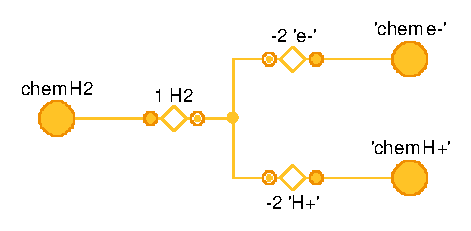
\includegraphics[width=0.5\linewidth]{4-HORD}}
    \label{fig:HOR}
  }\quad
  \subfloat[ORR ($4\timessep\s{e-} + 4\timessep\s{H+} + \s{O2} \rightarrow 2\timessep\s{H2O}$)]{
    \fbox{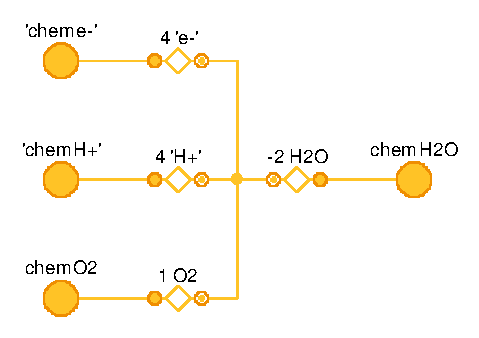
\includegraphics[width=0.5\linewidth]{4-ORRD}}
    \label{fig:ORR}
  }
  \caption{Diagrams of the reaction models}
  \label{fig:Reactions}
\end{figure}
 

\subsection{Electron Transfer and Charge Storage}

The \modelica{ElectronTransfer} model implements the Butler-Volmer equation (\ref{eq:Reaction}).  It includes advection and heat generation.  The heat is rejected to an \modelica{Inert} connector which is connected to the substrate (\n{C+}).  The Nernst equation is not implemented in this model (or any other model in the library) because the open circuit voltage is inherent in the properties of the species and their interconnection.

The \modelica{DoubleLayer} model stores and releases energy due to charge displacement across the electrolytic double layer.  Even though it is instantiated in the \modelica{graphite} phase (\autoref{sec:Phases}), it has its own volume (although small) which is introduced through an \modelica{Amagat} connector.  The  \modelica{DoubleLayer} model also has an \modelica{Inert} connector for translational and thermal exchange.  The electrons exit with either the velocity of that connector (typically zero) or the arrival velocity.  The first option, which is the default, implies that heat is generated; it is rejected through the same connector.  

The Modelica code and a table of parameters for \modelica{ElectronTransfer} and \modelica{DoubleLayer} are included in Sections~\ref{sec:FCSys_Chemistry_Electrochemistry_ElectronTransfer} and \ref{sec:FCSys_Chemistry_Electrochemistry_DoubleLayer}.


\subsection{Capillary Pressure}

Surface tension and capillary action are essential to remove liquid water from the cell.  The \modelica{Capillary} model applies capillary pressure between two \modelica{Amagat} connectors according to the Young-Laplace equation~\cite{Butt2003}.  It is instantiated within the \modelica{CapillaryVolume} model, where it yields a pressure difference between the liquid and the gas.  Since the water vapor is modeled as an ideal gas and the liquid has constant volume, the pressure difference shifts the saturation pressure according to the Kelvin equation~\cite{Butt2003}.

The Modelica code and a table of parameters for the \modelica{Capillary} model is included in \autoref{sec:FCSys_Chemistry_Capillary}.


\FloatBarrier % Flush the floats.
\section{Phases}
\label{sec:Phases}

\begin{contextbox}
  Related sections of the documentation:
  \vspace{0.5\baselineskip}

  \renewcommand{\arraystretch}{1.5}
  \begin{tabular}{ll}
    \docrow{sec:FCSys_Phases_PartialPhase}{FCSys.Subregions.Phases.PartialPhase}
  \end{tabular}
\end{contextbox}

There are four phase models---one for gas, one for liquid, and two different solids.  The \modelica{Gas} model contains \n{H2}, \n{H2O}, \n{N2}, and \n{O2}.  \modelica{Liquid} contains \n{H2O}.  \modelica{Graphite} contains \n{C+} and \n{e-}; \modelica{Ionomer} contains \n{H+}, \n{H2O}, and \s{SO3-} (abbreviation for \s{C19HF37O5S-}).  The species are conditionally included so that the \modelica{Gas} model can be used in both the anode (with \n{N2} and \n{O2} removed) and the cathode (with \n{H2} removed).

Within a phase, the species are combined according to Dalton's law.  The species exert forces on each other and exchange heat according to the diffusive exchange equations (\ref{eq:TranslationalDiffusiveExchange} and \ref{eq:ThermalDiffusiveExchange}).  By setting the independence factors to zero, it is possible to impose the assumption that the temperature or any component of velocity is equal among the species.  This causes the translation tool to simplify the model via index reduction.  
% Assuming the two phase flow of \n{FC} channel can be characterized as slug flow, the \n{VOF} method is appropriate (one set of momentum equations for all phases within each region) \cite[Ch. 23]{Fluent6.3}.

\autoref{fig:Phases} shows the diagrams of the phases.  All the phases have boundary bus connectors (\modelica{xNegative}, \modelica{xPositive}, etc.) to connect to adjacent subregions.  Species are labeled by their chemical formula when they are connected to the bus.  Each phase also has an \modelica{amagatDalton} adapter between Dalton's law (which is applied within the phase) and Amagat's law, which is applied among phases via the \modelica{amagat} connector.  The phases have \modelica{inter} connectors for inter-phase translational and thermal exchange.  Internal nodes (e.g., \modelica{commonExch}) are included as required for translational and thermal exchange within each phase.  Finally, the phases have chemical connectors (e.g., \modelica{chemH2O}) for chemical reactions and phase change among the phases.  The graphite phase (\autoref{fig:Graphite}) has a model for electron transfer (\modelica{electronTransfer}) and an optional electrolytic double layer capacitance (\modelica{doubleLayer}). 

\begin{figure}[htbp]
  \subfloat[Gas]{
    \fbox{\lwincludegraphics[width=0.82\linewidth]{4-Phases-GasD}}
    \label{fig:Gas}
  }\quad
  \subfloat[Graphite]{
    \fbox{\lwincludegraphics[width=8cm]{4-Phases-GraphiteD}}
    \label{fig:Graphite}
  }\quad
  \subfloat[Liquid]{
    \fbox{\lwincludegraphics[height=5cm]{4-Phases-LiquidD}}
    \label{fig:Liquid}
  }
  \phantomcaption
\end{figure}

\begin{figure}[htb]
  \ContinuedFloat
  \subfloat[Ionomer]{
    \fbox{\lwincludegraphics[width=10.2cm]{4-Phases-IonomerD}}
    \label{fig:Ionomer}
  }
  \caption{Diagrams of the phases}
  \label{fig:Phases}
\end{figure}


\autoref{fig:PhaseGUI} shows the parameter dialog for the gas phase.  The species can be enabled or disabled and their settings can be changed by opening the sub-dialogs shown in \autoref{fig:SpeciesGUI}.

\begin{figure}[htbp]
  \gui{4-GUI-Gas-General}
  \caption{Parameter dialog for the gas phase}
  \label{fig:PhaseGUI}
\end{figure}


\FloatBarrier % Flush the floats.
\section{Subregions}
\label{sec:Subregions}

\begin{contextbox}
  Related sections of the documentation:
  \vspace{0.5\baselineskip}

  \renewcommand{\arraystretch}{1.5}
  \begin{tabular}{ll}
    \docrow{sec:FCSys_Subregions_Subregion}{FCSys.Subregions.Subregion}
  \end{tabular}
\end{contextbox} 

The smallest unit of spatial discretization is the \modelica{Subregion} model, which is shown in \autoref{fig:Subregion}.  It contains instances of the phase models---\modelica{liquid}, \modelica{gas}, \modelica{graphite}, and \modelica{ionomer}.  They are connected to the \modelica{volume} model, which imposes the total volume of the subregion and applies capillary pressure between the gas and the liquid (see \autoref{sec:Chemistry}).  All of the phases are connected to the internal \modelica{commonExch} node for translational and thermal exchange.  The gas and liquid have an additional means of diffusive exchange via the \modelica{gasLiq} node.  Although not shown in the diagram, the chemical connectors of the phases are connected to the chemical reactions (\modelica{HOR} and \modelica{ORR}) described in \autoref{sec:Chemistry}.  The chemical connectors are directly connected for phase change---between gas and liquid and between gas and the ionomer (also not shown in the diagram). 

\begin{figure}[htbp]
  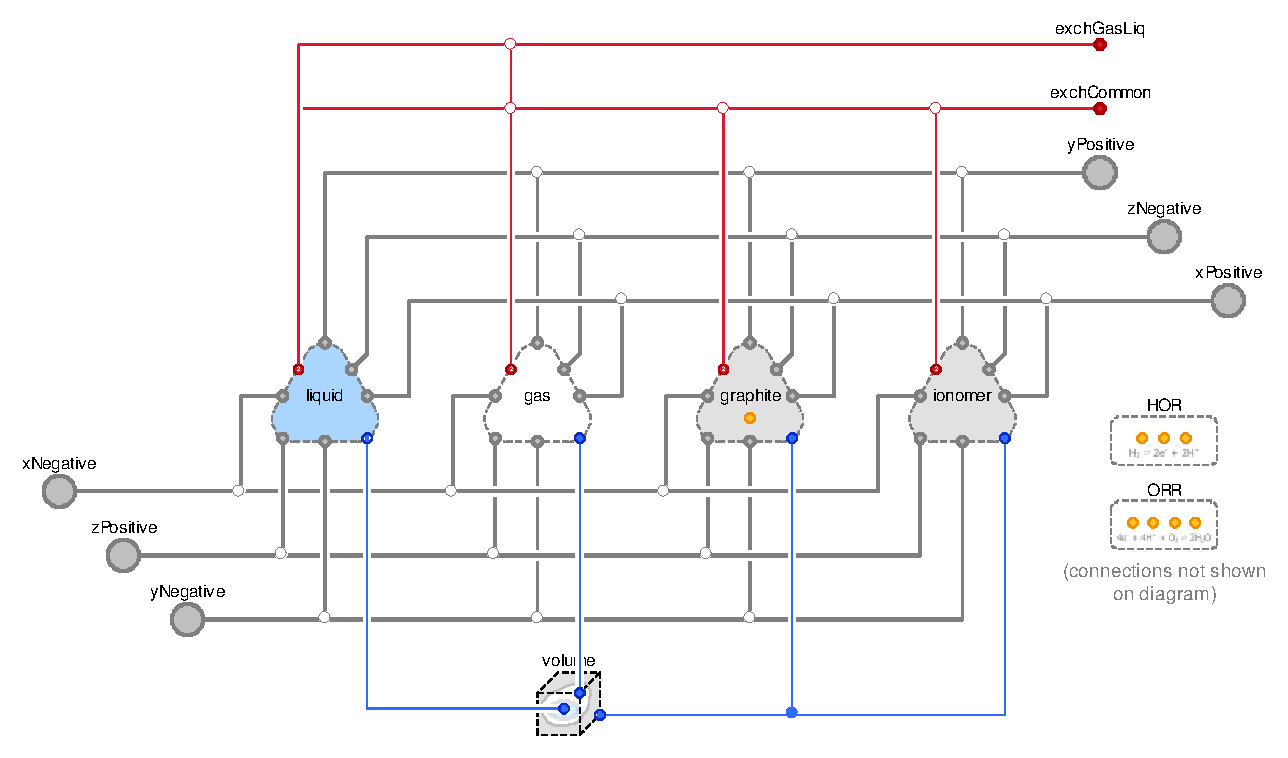
\includegraphics[width=\linewidth]{4-SubregionD}%
  \caption{Diagram of a subregion}
  \label{fig:Subregion}
\end{figure}

The external connectors (\modelica{xNegative}, \modelica{xPositive}, etc.) represent the boundaries of the rectilinear control volume.   Phases are labeled (\modelica{gas}, \modelica{liquid}, etc.) when they are connected to the boundaries.  By default, the \modelica{Subregion} model is \n{3D}.  However, assumptions may be applied via the Boolean parameters shown in \autoref{fig:SubregionGUIAssumptions} (and listed in \autoref{tab:FCSys_Subregions_Subregion-params}) to individually eliminate components of translational momentum and pairs of boundary connectors.  The settings for the phases (\autoref{fig:PhaseGUI}) can be accessed through the main tab of the parameter dialog shown in \autoref{fig:SubregionGUIGeneral}.

\begin{figure}[htbp]
  \subfloat[General parameters]{
    \gui{4-GUI-Subregion-General}
    \label{fig:SubregionGUIGeneral}
  }\quad
  \subfloat[Assumptions]{
    \gui{4-GUI-Subregion-Assumptions}
    \label{fig:SubregionGUIAssumptions}
  }
  \caption{Parameter dialog for a subregion}
  \label{fig:SubregionGUI}
\end{figure}


\FloatBarrier % Flush the floats.
\section{Regions\slash{}Layers}

\begin{contextbox}
  Related sections of the documentation:
  \vspace{0.5\baselineskip}

  \renewcommand{\arraystretch}{1.5}
  \begin{tabular}{ll}
    \docrow{sec:FCSys_Regions_AnCLs_AnCL}[sec:FCSys_Regions_Region]{FCSys.Regions.*}
  \end{tabular}
\end{contextbox}

 The layers of the cell are represented by regions which contain \n{3D} arrays of subregions.  Each layer is an extension of a base \modelica{Region} model with the appropriate settings (e.g., geometry and selection of species).   The grid is fixed and rectilinear but may have irregular spacing.  \autoref{fig:RegionImplemented} shows the diagram of the \modelica{Region} model.  The \modelica{subregions} icon in the center actually represents an array of subregions (which defaults to \num{1 x 1 x 1}).  The interconnections are automatically included.  \autoref{fig:RegionExpanded} shows the equivalent form for a \num{2 x 2 x 2} array, without the external connectors.  The boundaries (\modelica{xNegative}, \modelica{xPositive}, etc.) are \n{2D} arrays of bus connectors.


\begin{figure}[htbp]
  \subfloat[As implemented]{
    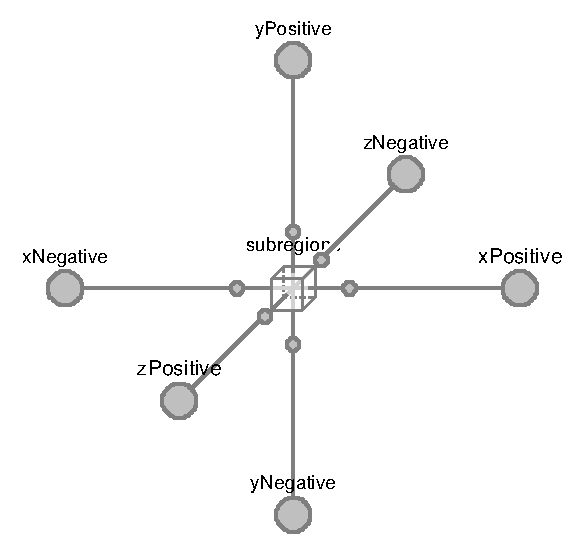
\includegraphics[width=0.46\linewidth]{4-RegionD}
    \label{fig:RegionImplemented}
  }\quad
  \subfloat[Expanded to show interconnections]{
    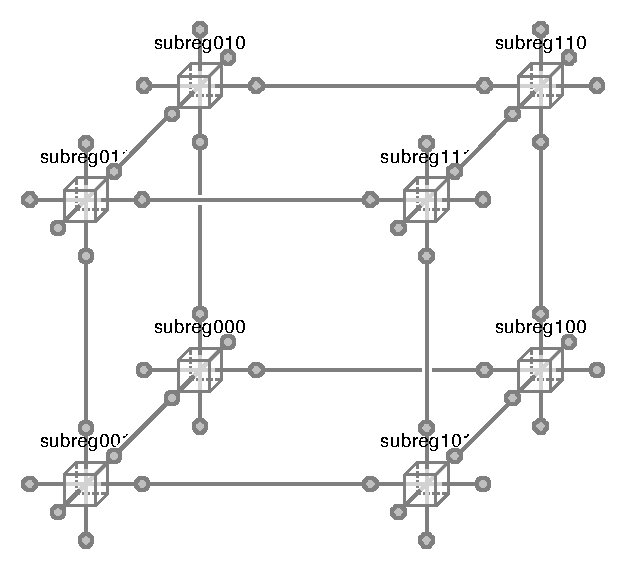
\includegraphics[width=0.46\linewidth]{4-MatrixD}
    \label{fig:RegionExpanded}
  }
  \caption{Diagrams of a region}
  \label{fig:Region}
\end{figure}


\autoref{fig:RegionGUI} shows the parameter dialog for a region model---the anode flow plate.  The lengths (\s{L}[_y], \s{L}[_y], and \s{L}[_z]) are one-dimensional arrays that contain the lengths of the subregions along the corresponding dimensions.  Only the z-axis boundaries are optional (\autoref{fig:RegionGUIAssumptions}) because the x- and y-axis boundaries are required due to the cell geometry.


\begin{figure}[htbp]
  \subfloat[General parameters]{
    \gui{4-GUI-AnFP-General}
    \label{fig:RegionGUIGeneral}
  }\quad
  \subfloat[Assumptions]{
    \gui{4-GUI-AnFP-Assumptions}
    \label{fig:RegionGUIAssumptions}
  }
  \caption{Parameter dialog for the anode flow plate}
  \label{fig:RegionGUI}
\end{figure}


\FloatBarrier % Flush the floats.
\section{Assemblies\slash{}Cells}


As shown in \autoref{fig:CellDiagrams}, the diagram of the fuel cell model (\autoref{fig:CellModel}) corresponds directly to the physical structure of the cell (\autoref{fig:Cell} and \autoref{fig:CellFlows}).  \autoref{fig:SimpleCellModel} shows a version of the cell model with nearly minimal complexity given the present modeling framework.  Its gas diffusion and catalyst layers are integrated (\modelica{anCGDL} and \modelica{anCGDL}) and all the species have the same temperature in every subregion, regardless of phase.

By default, each layer only contains one subregion (i.e., 1D model), but this can be increased.  The number of sets of subregions and the lengths of the subregions in the y and z directions (along and across the channel) are the same for all of the layers.  However, the number of sets of subregions and the lengths of the subregions are independent in the x direction (through the cell).


\begin{figure}[htbp]
  \subfloat[Physical structure]{
    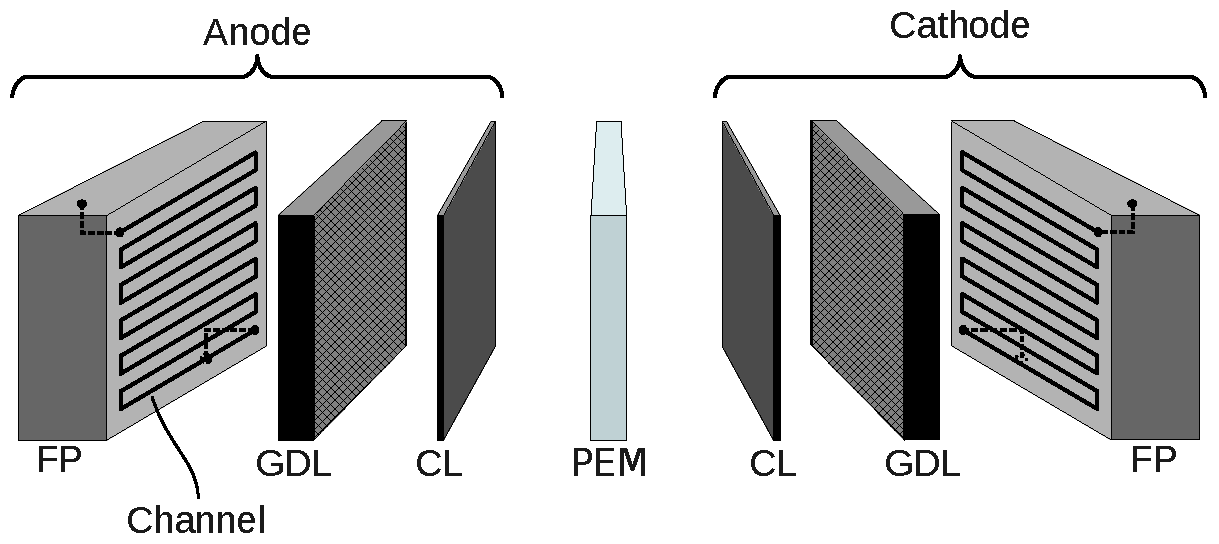
\includegraphics[width=0.75\linewidth]{1-Cell}
    \label{fig:Cell}
  }\quad
  \subfloat[Standard model diagram]{
    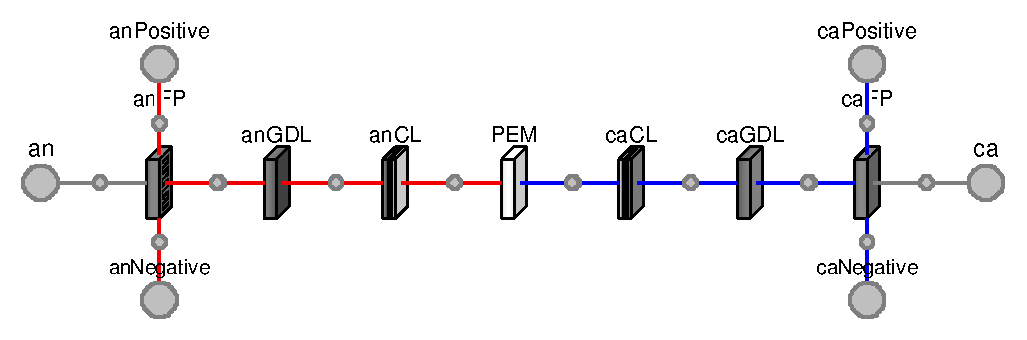
\includegraphics[height=5cm]{4-CellD}
    \label{fig:CellModel}
  }\quad
  \subfloat[Simplified model diagram]{
    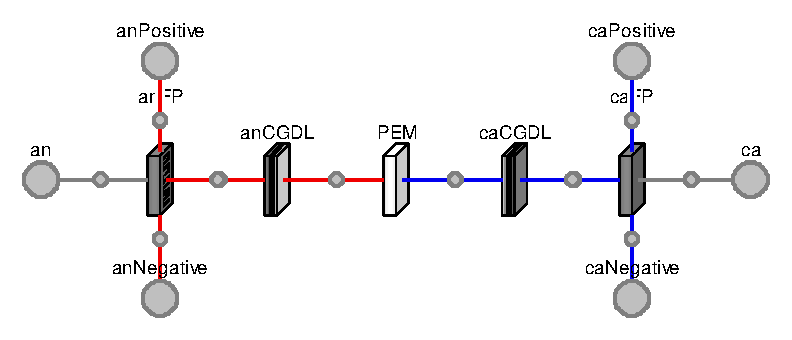
\includegraphics[height=5cm]{4-SimpleCellD}
    \label{fig:SimpleCellModel}
  }
  \caption{Single-cell \n{PEMFC}}
  \label{fig:CellDiagrams}
\end{figure}



\FloatBarrier % Flush the floats.
\section{Test Stand}
\label{sec:TestStand}

\begin{contextbox}
  Related section of the documentation:
  \vspace{0.5\baselineskip}

  \renewcommand{\arraystretch}{1.5}
  \begin{tabular}{ll}
    \docrow{sec:FCSys_Assemblies_Cells_Examples_TestConditions}[sec:FCSys_Assemblies_Cells_Examples_TestStand]{FCSys.Assemblies.Cells.Examples.*}
    \docrow{sec:FCSys_Conditions_Environment}{FCSys.Conditions.Environment}
  \end{tabular}
\end{contextbox}

The highest physical level of the library is the \modelica{TestStand} model, which applies boundary conditions to the fuel cell.  As shown in \autoref{fig:TestStandD}, there are four boundary conditions for the channels---a source and a sink for both the anode and cathode.  The cell model is bidirectional, so the choice of inlet and outlet can be switched via \modelica{anRouter} and \modelica{caRouter}.   By default, the \modelica{anBC} and \modelica{caBC} models apply uniform temperature to the exterior of the flow plates along the x axis.  An electrical model from the Modelica Standard Library~\cite{ModelicaSL3.2} is connected as a load to the first (1, 1) segment of the cell in the yz plane via the \modelica{anAdapt} and \modelica{caAdapt} adapters.  The default load is a current ramp (\modelica{Modelica.Electrical.Analog.Sources.CurrentRamp}).  

Besides the electrical load, the following key conditions are adjustable:
\begin{enumerate*}
  \item Temperature of the end plates and reactant sources
  \item Relative humidities of the reactant sources (independently adjustable)
  \item Fixed or stoichiometrically-varying reactant flow rates (independently adjustable)
  \item Fraction of \n{N2} in the cathode supply
  \item Pressures of the reactant sinks
  \item Optional inclusion of liquid water
\end{enumerate*}

\begin{figure}[htbp]
  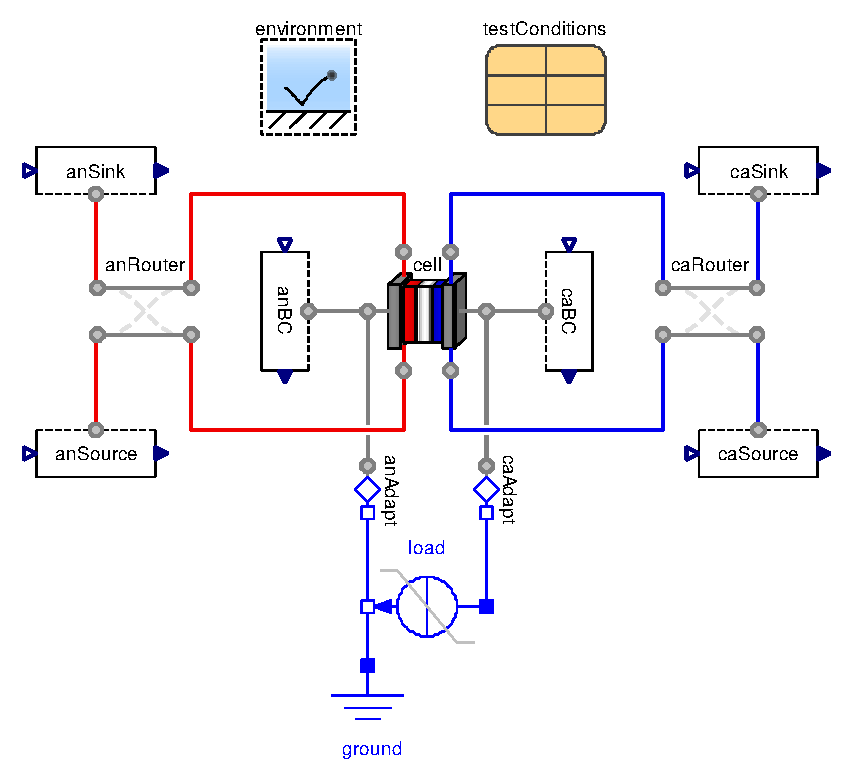
\includegraphics[width=0.8\linewidth]{4-TestStandD}%
  \caption{Diagram of the fuel cell test stand}%
  \label{fig:TestStandD}%
\end{figure}



\FloatBarrier % Flush the floats.
\section{Summary}

This chapter described the implementation of the model library in the Modelica language~\cite{Modelica3.3}.  It provided references to the more detailed documentation in \autoref{chap:Doc}.  The model library, like this chapter, builds from low-level classes such as types and constants to high-level classes such as the fuel cell model.  The models are highly modular and reconfigurable.  In the next chapter (\autoref{chap:Basic}), we will provide basic examples before exercising the full fuel cell model in \autoref{chap:Cell}.



  \chapter{Basic Examples}
  \label{chap:Basic}
  \glsresetall

% Don't show subsections in the TOC.
\addtocontents{toc}{\protect\setcounter{tocdepth}{1}}

The purpose of this chapter is to an provide initial, low-level validation of the model library.  It presents some basic examples of the model introduced in Chapters~\ref{chap:Fundamentals} and~\ref{chap:Implementation}.  Each section begins with an introduction of the physical conditions and assumptions.  Then, simulation results are shown and discussed.  Most of the examples in this chapter are not intended to be representative of a fuel cell.  However, the last two examples demonstrate phase change processes which are scaled so that the time constants roughly correspond to a \n{PEMFC}.

It is significant that all of the following examples---from gas dynamics to electrical con\-duction---were generated from the same working model (\modelica{Subregion}), only instantiated with various geometries and initial and boundary conditions.  The models of solids, liquid water, gases, electrons, and protons are different only in their material properties and default assumptions, all of which are configurable.

In addition to these examples, a comprehensive package of test models was created and simulated  to verify the thermodynamic and transport properties of the fluids against~\cite{Moran2004} and~\cite{Incropera2002}.  Also, the physical constants were verified against~\cite{NIST2010}.

The results of each example begins with statistics about the model and its simulation.  The models contain a number of variables, some of which are time-varying.  The number of states is the number of time derivatives that are algebraically independent.  It is the number of unique ways that energy can be introduced and stored in a model (enthalpy of formation between phases, boundary work, energy due to charge displacement, kinetic energy along each axis, and internal energy).  At a given time, the state variables can be considered known.  The size of each system of equations is the number of algebraically coupled equations that must be solved from the known variables, which include the states and time-constant variables.  The systems of equations may be linear or nonlinear.

Before simulation, a model must be translated.  This includes the process of parsing the Modelica syntax, flattening the object-oriented code, manipulating and sorting the equations, tearing systems of equations, and compiling the result with links to the solvers and integrator.  The models were translated and simulated on a Samsung ATIV Book 8 laptop computer (Intel Core i7 3635QM @ \SI{2.40}{GHz}, \SI{8}{GB}~RAM DDR3 @ \SI{1600}{MHz}, \SI{5400}{RPM}~hard drive) running Windows~8.1 and Dymola~2014.  The hardware represents technology that is approximately one year old (processor introduced 3\textsuperscript{rd} quarter 2012). 

The default Dymola settings were used, including the \n{DASSL} and 500 output intervals, except:
\begin{enumerate*}
  \item \modelica{GuardedSqrt = false}
  \item \modelica{ImprovedPackageConstants = true}
  \item \modelica{IncludeLibrariesForSimulink = false}
  \item \modelica{SubstituteVariablesUsedOnce = true}
\end{enumerate*}
Most models were simulated with an integration tolerance of \num{E-4}, but this was increased as needed.  The following debugging options were enabled which may have affected the translation and compilation time:
\begin{enumerate*}
  \item \modelica{CheckUnits = false}
  \item \modelica{LogDefaultInitialConditions = true}
  \item \modelica{LogStateSelection = true}
  \item \modelica{OutputCPUtime = true}
  \item \modelica{OutputModelicaCode = true}
  \item \modelica{OutputModelicaCodeWithAliasVariables = true}
  \item \modelica{StoreProtectedVariables = true}
\end{enumerate*}



\section{Internal Flow}
\label{sec:InternalFlow}

This example compares the model to Poiseuille's law~\cite{Cengel2006} for pressure drop along a pipe under laminar flow.  Poiseuille's law was derived from the model equations in \autoref{sec:TransverseTransport}, so this example is partly a test that the implementation performs as expected.  It also demonstrates inertance and thermal dynamics.

\subsection{Conditions}

Liquid water is forced along the long axis through a rectangular $\SI{1}{m}\times\SI{1}{mm}\times\SI{1}{mm}$ subregion as shown in \autoref{fig:InternalFlow}.  In addition to a large-signal volumetric flow rate of \SI{1.5}{cm^3/s}, there is a small sinusoidal signal with an amplitude of \SI{0.3}{cm^3/s} and a frequency of \SI{1}{Hz}.  This corresponds to an area-average (plug flow equivalent) velocity of $1.5\pm$\SI{0.3}{m/s} as shown in \autoref{fig:InternalFlowRate}. % and a space velocity of $1.5\pm$\SI{0.3}{s^{-1}}.  
A no-slip (zero velocity) condition is applied around the perimeter.  The fluid source is held at \SI{25}{\celsius}.  There is no thermal conduction across the outlet (only advection) or around the perimeter.  

\begin{figure}[htbp]
  \subfloat[Physical domain]{
    \fbox{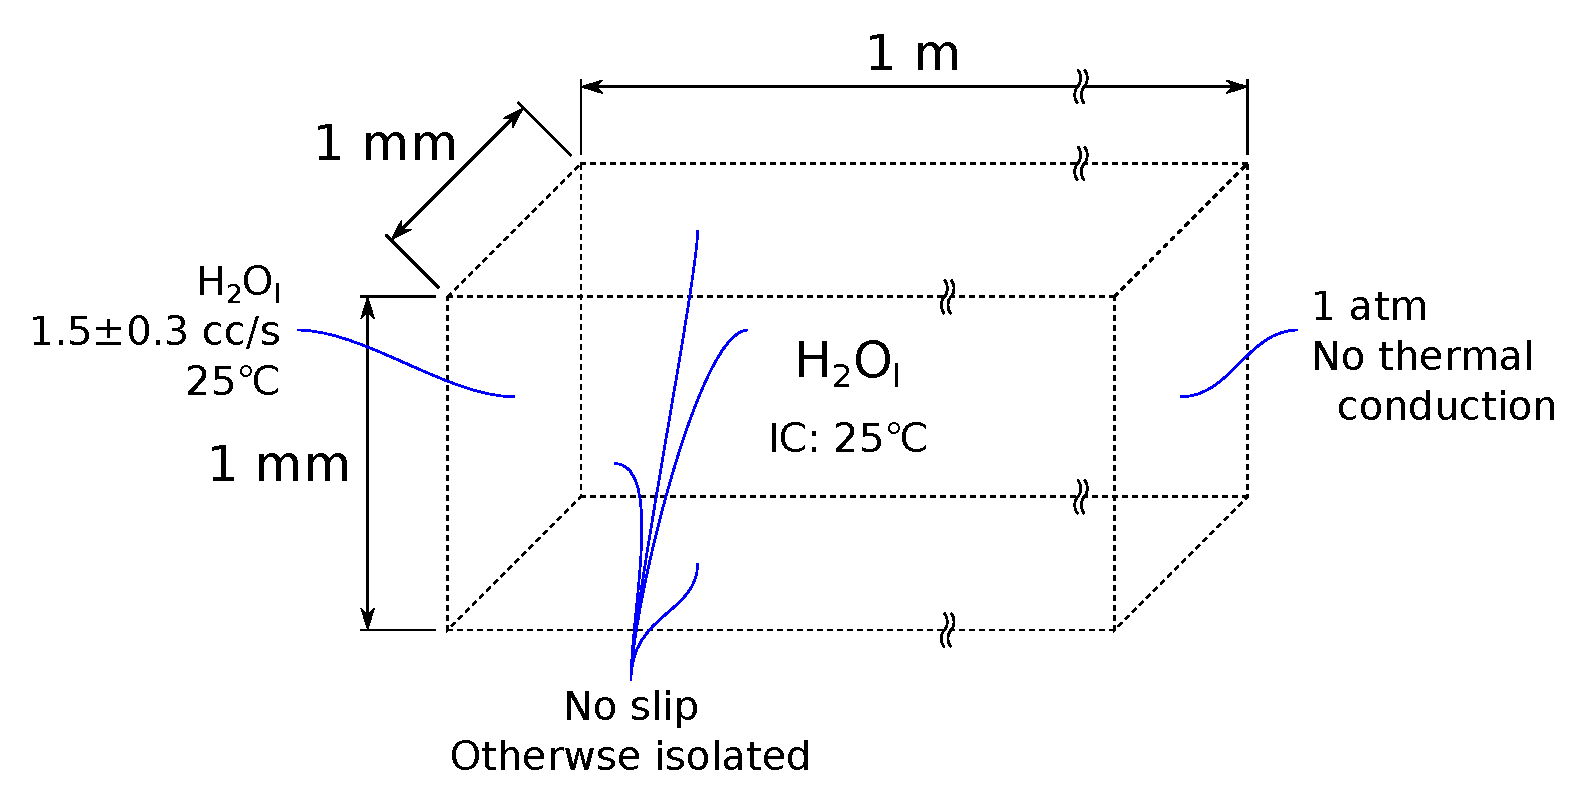
\includegraphics[width=\linewidth]{5-InternalFlow}}%
    \label{fig:InternalFlowPhysical}
  }\\
  \subfloat[Model]{
    \fbox{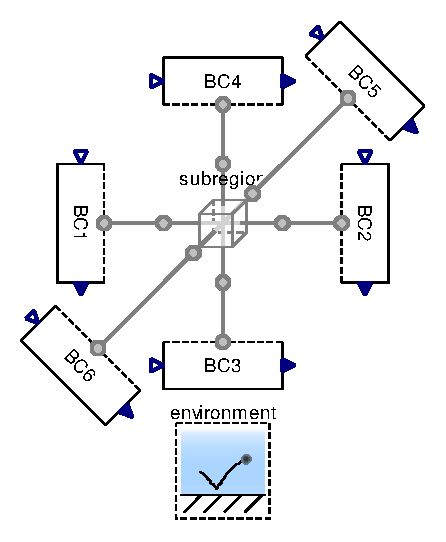
\includegraphics[width=0.6\linewidth]{5-InternalFlowD}}%
    \label{fig:InternalFlowDiagram}
  }
  \caption{Configuration of the internal flow example}\glsadd{IC}
  \label{fig:InternalFlow}
\end{figure}

\begin{figure}[htbp]
  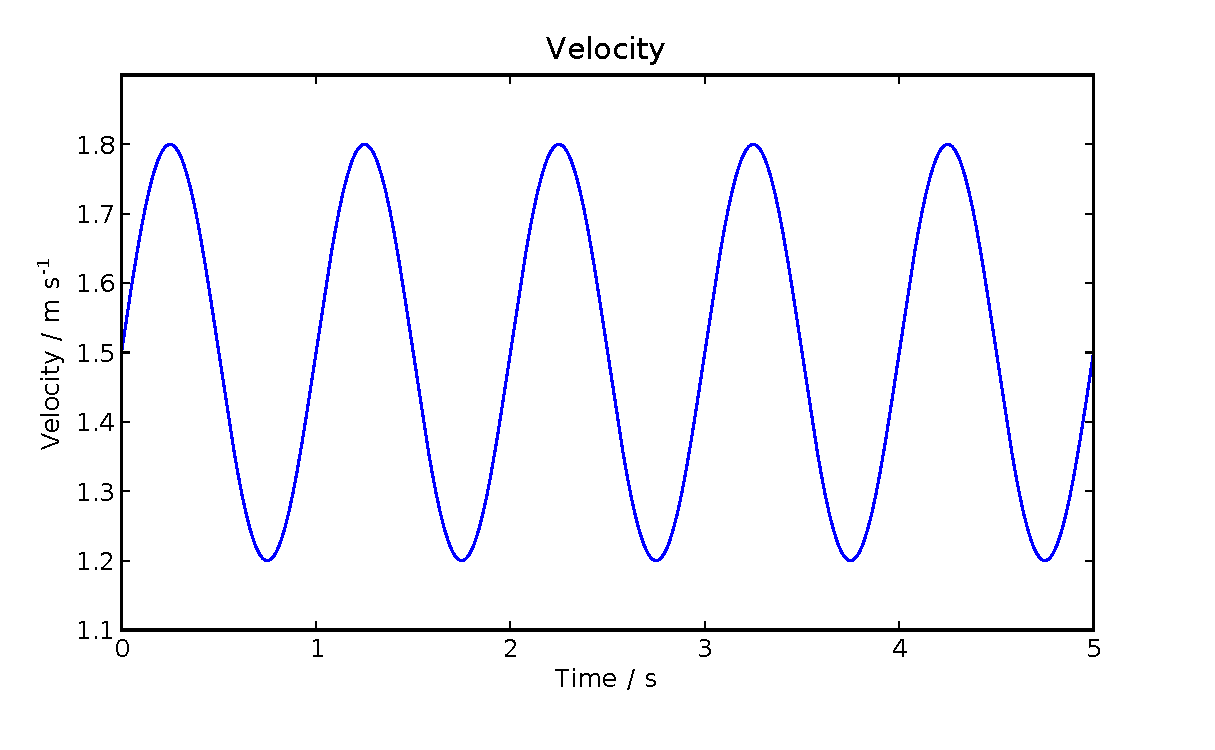
\includegraphics[width=\linewidth]{Results/Basic/InternalFlow/1/Velocity}%
  \caption{Fluid velocity for the internal flow example}%
  \label{fig:InternalFlowRate}
\end{figure}

The Reynolds number varies from 1400 to 2100; therefore, laminar flow is expected.  The translational Nusselt number for the liquid water is set to four ($\s{Nu}[_Phi] = 4$, the default), which is appropriate for laminar flow with a single subregion over the cross section.

\subsection{Results and Discussion}

\begin{table}[h]
  \caption{Modeling and simulation statistics for the internal flow example}
  \begin{singlespaced}%
    \begin{tabular}{llll}%
      \toprule 
      & With analysis & Without analysis \\
        \midrule
      Number of variables & 516 & 474 \\
      Number of time-varying variables & 104 & 55 \\
      Number of states & 1 & 1 \\
      Sizes of the nonlinear systems of equations & None & None \\
      Sizes of the linear systems of equations & 4 sets of 2 & 4 sets of 2 \\
      Translation time & \SI{3}{s} & \SI{1}{s} \\
      Simulation time & \SI{0.007}{s} & \SI{0.007}{s} \\
      \bottomrule
    \end{tabular}
  \end{singlespaced}
\end{table}



The modeling and simulation statistics are listed above.  The model contains a fairly large number of variables (516) given the simple physical system.  The object-oriented nature of the model introduces overhead in terms of the number of variables.  Some of the variables (8\% of all variables and 47\% of the time-varying variables) are outputs that are purely for analysis.  They can be disabled without affecting the behavior.  Roughly one fifth of the variables are time-varying.  The model contains only one state: temperature.  Velocity is not a state since the translational dynamics are imposed directly by the boundary conditions (prescribed volumetric flow rate) and the fluid is incompressible.  There are no time-varying systems of algebraic equations after manipulation.  The model simulates very quickly (\SI{7}{ms}). The analysis variables have negligible effect on the simulation time.  Translation takes over 400~times longer than simulation.  However, the model may be re-simulated with various parameter settings without re-translating it.

\autoref{fig:InternalFlowPressure} shows the difference in thermodynamic pressure across the subregion.  Due to inertance, the pressure difference of the model leads the pressure difference according to Poiseuille's law and has a slightly larger amplitude.  The effect of inertance becomes more prominent at higher frequencies and less so at lower frequencies.

\begin{figure}[htbp]
  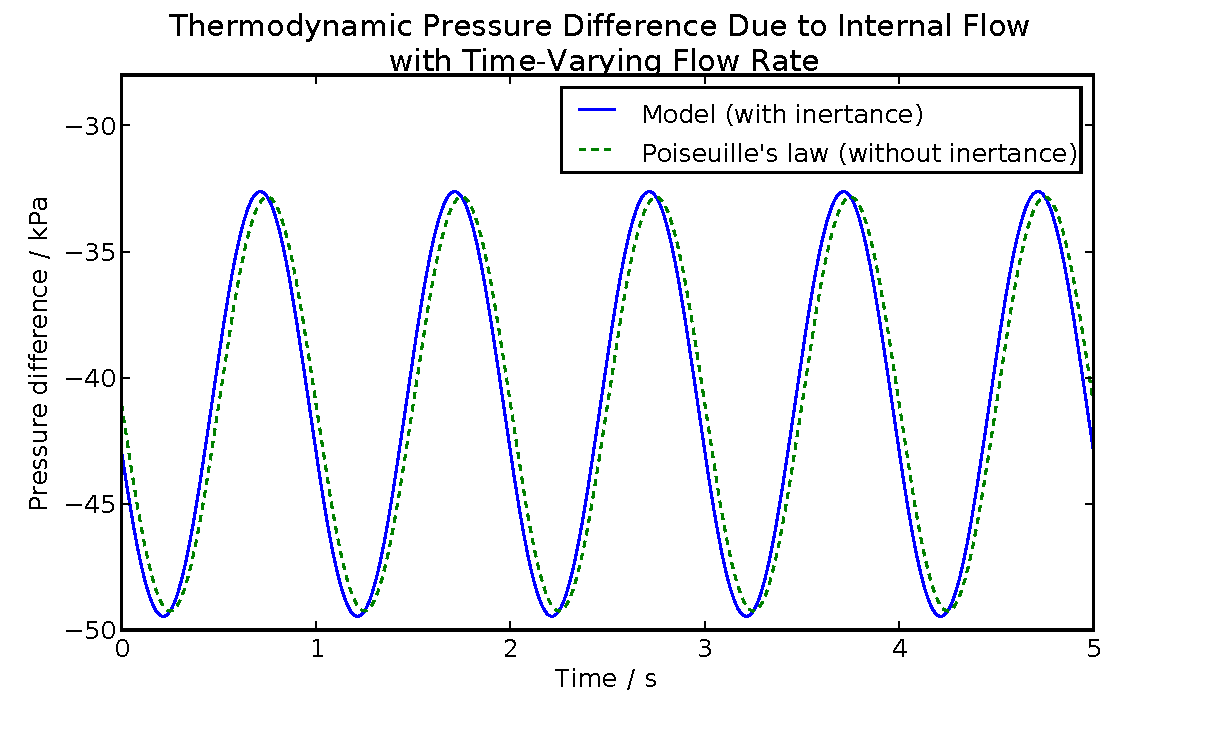
\includegraphics[width=\linewidth]{Results/Basic/InternalFlow/1/Pressure}%
  \caption{Dynamic pressure difference under internal flow}%
  \label{fig:InternalFlowPressure}
\end{figure}

The temperature of the fluid in the subregion increases due to viscous dissipation as shown in \autoref{fig:InternalFlowTemperature}.  However, the temperature rise is only \SI{9}{mK} (to \SI{25.009}{\celsius}) because the rate of heat generation is much smaller than the rate of enthalpy flow from the source.  The increase is so slight that the simulation tolerance must be increased from $10^{-4}$ (the default) to $10^{-8}$ in order to distinguish it from the solver error.  The temperature increases with a first-order dynamic response.  A sinusoidal temperature variation is superimposed due to the small-signal part of the flow rate.  

\begin{figure}[htbp]
  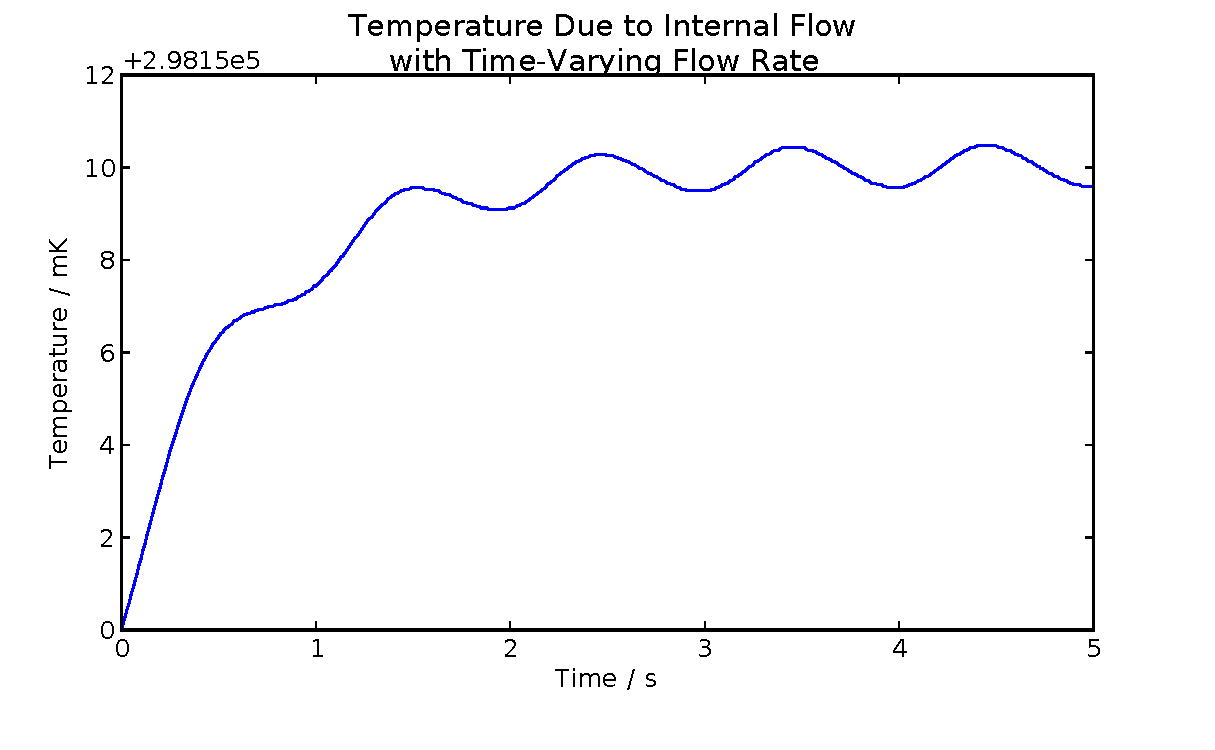
\includegraphics[width=\linewidth]{Results/Basic/InternalFlow/1/Temperature}%
  \caption{Thermal transients due to viscous dissipation in internal flow}%
  \label{fig:InternalFlowTemperature}
\end{figure}


\FloatBarrier % Flush the floats.
\section{Echo}

This example shows the dynamics of compressible flow in the model.  A pressure wave reflects between the external boundaries of adjacent subregions.  The effect of the discretization scheme can be seen.  The key model equations are material transport (\autoref{eq:MaterialTransport}) and material conservation (\autoref{eq:MaterialBalance}).

\subsection{Conditions}

Two cubic \SI{1}{cm^3} subregions containing \n{H2} are arranged side-by-side with an initial pressure difference of \SI{100}{Pa} as shown in \autoref{fig:Echo}.  The \modelica{subregions} array of models is removed and bypassed upon translation because there are only two subregions.  Both subregions are initialized to \SI{25}{\celsius}.  All external boundaries are isolated (i.e., closed, adiabatic, and free-slip).  The model is evaluated with upstream discretization and with the central difference scheme.

\begin{figure}[htbp]
  \subfloat[Physical domain]{
    \fbox{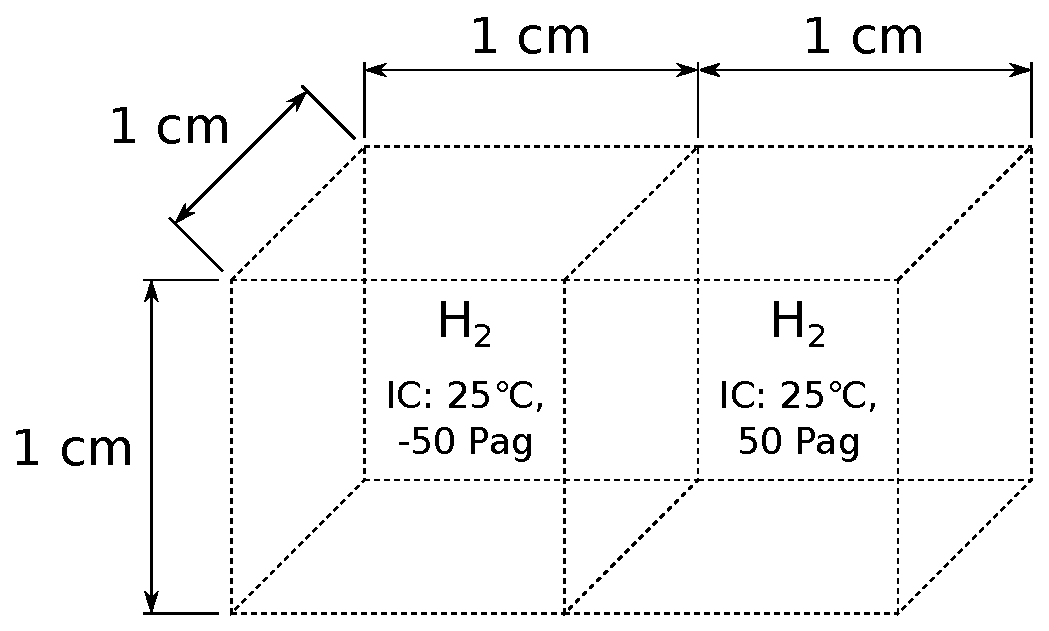
\includegraphics[width=3in]{5-Echo}}%
    \label{fig:EchoPhysical}
  }\vspace*{-1.6cm}\\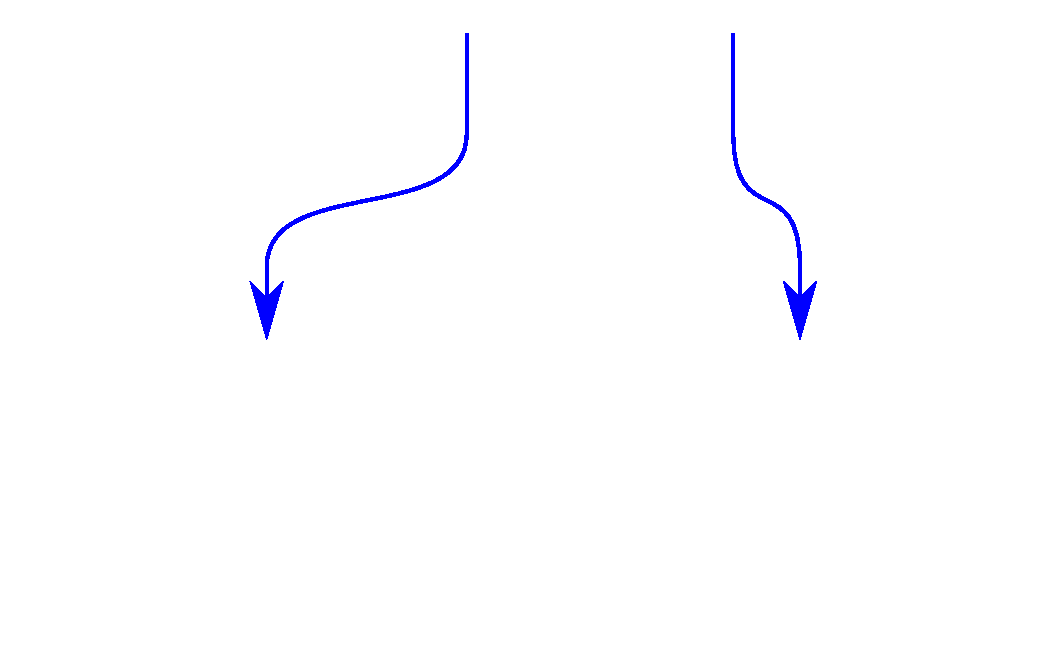
\includegraphics[width=4in]{5-EchoLink}\vspace*{-4cm}\\
  \subfloat[Model]{
    \fbox{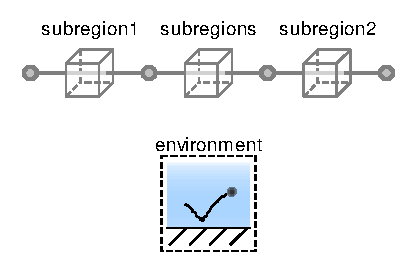
\includegraphics[width=0.6\linewidth]{5-EchoD}}%
    \label{fig:EchoDiagram}
  }
  \caption{Configuration of the echo example (\s{H2} gas with an initial pressure difference)}
  \label{fig:Echo}
\end{figure}

\subsection{Results and Discussion}

\begin{table}[h]
  \caption{Modeling and simulation statistics for the echo example}
  \begin{singlespaced}%
    \begin{tabular}{llll}%
      \toprule 
      & Upstream & Central \\
      & discretization & difference \\
        \midrule
      Number of variables & 488 & 488 \\
      Number of time-varying variables & 122 & 118 \\
      Number of states & 5 & 5 \\
      Sizes of the nonlinear systems of equations & None & None \\
      Sizes of the linear systems of equations & 2 sets of 2 & 2 sets of 2 \\
      Translation time & \SI{3}{s} & \SI{3}{s} \\
    Simulation time & \SI{0.011}{s} & \SI{0.010}{s} \\
      \bottomrule
    \end{tabular}
  \end{singlespaced}
\end{table}



The model simulates slightly faster (9\%) with the central difference scheme, although the time may not be significant given the uncertainty due to the overhead of the operating system.  These models are roughly the same as the internal flow model (\autoref{sec:InternalFlow}) in terms of complexity, translation time, and simulation time.

As shown in \autoref{fig:EchoPressureDamped}, the model exhibits oscillations due to the coupled dynamics of compression and translation.  This is essentially a mass-spring-damper system.  The damping is due to irreversible material compression and expansion (\autoref{eq:MaterialTransport}).  If the continuity (\s{zeta}) is set to zero, there is no damping.  This case is shown in \autoref{fig:EchoPressureNoDamping}.  The outer boundaries have the same temperature as the nearest subregion.  The period of oscillation is \SI{0.0338}{ms}, which corresponds to a wave velocity of \SI{592}{m/s}.  This is roughly half of the speed that is expected for \n{H2} as an ideal gas at \SI{25}{\celsius} with an adiabatic index of approximately 1.4.  Currently, the reason for the discrepancy is unknown.  The plots in \autoref{fig:EchoPressure} are from the case where upstream discretization is used, but the central difference scheme gives identical results.  The common boundary remains at the average pressure in both cases.  An upstream bias is applied to the balance between pressure gradients and irreversible compression, but the associated P\'eclet number is very small even with the significant damping evident in \autoref{fig:EchoPressureDamped}.  For incompressible fluids, the damping and the P\'eclet number is exactly zero.

\begin{figure}[htbp]
  \subfloat[Default damping]{
    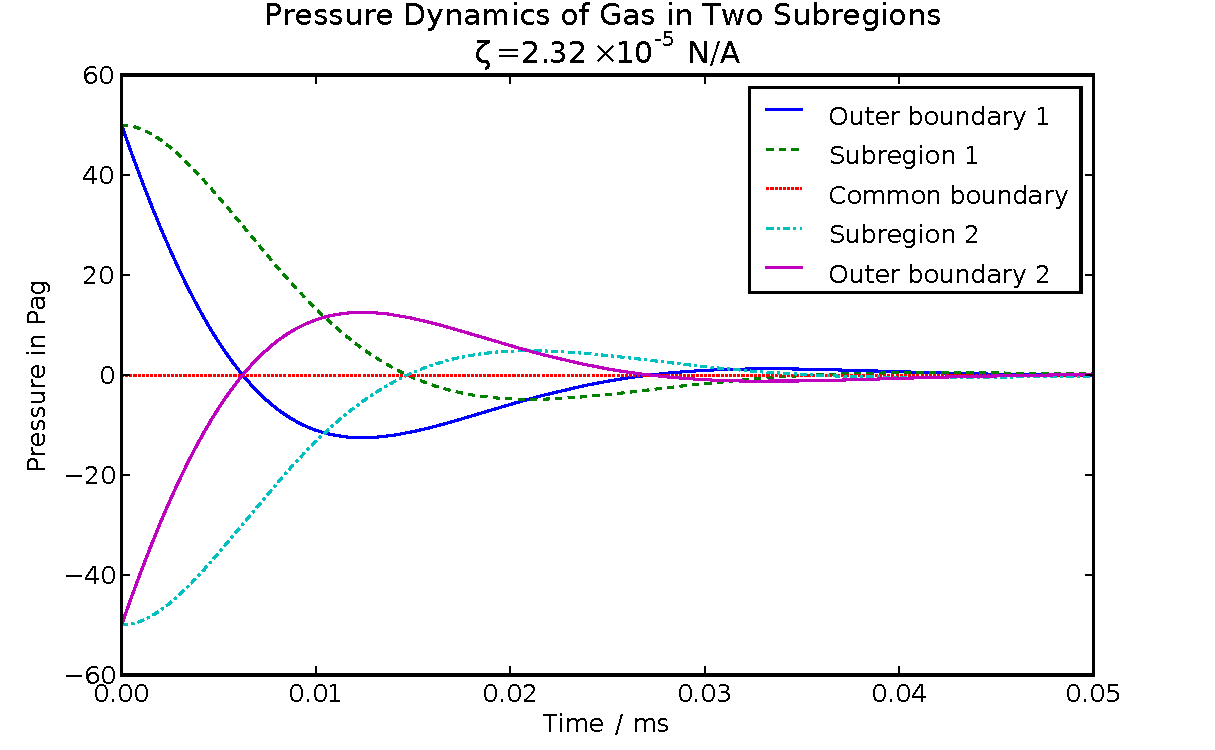
\includegraphics[width=\linewidth]{Results/Basic/Echo/2/Pressure}%
    \label{fig:EchoPressureDamped}
  }\quad
  \subfloat[No damping]{
    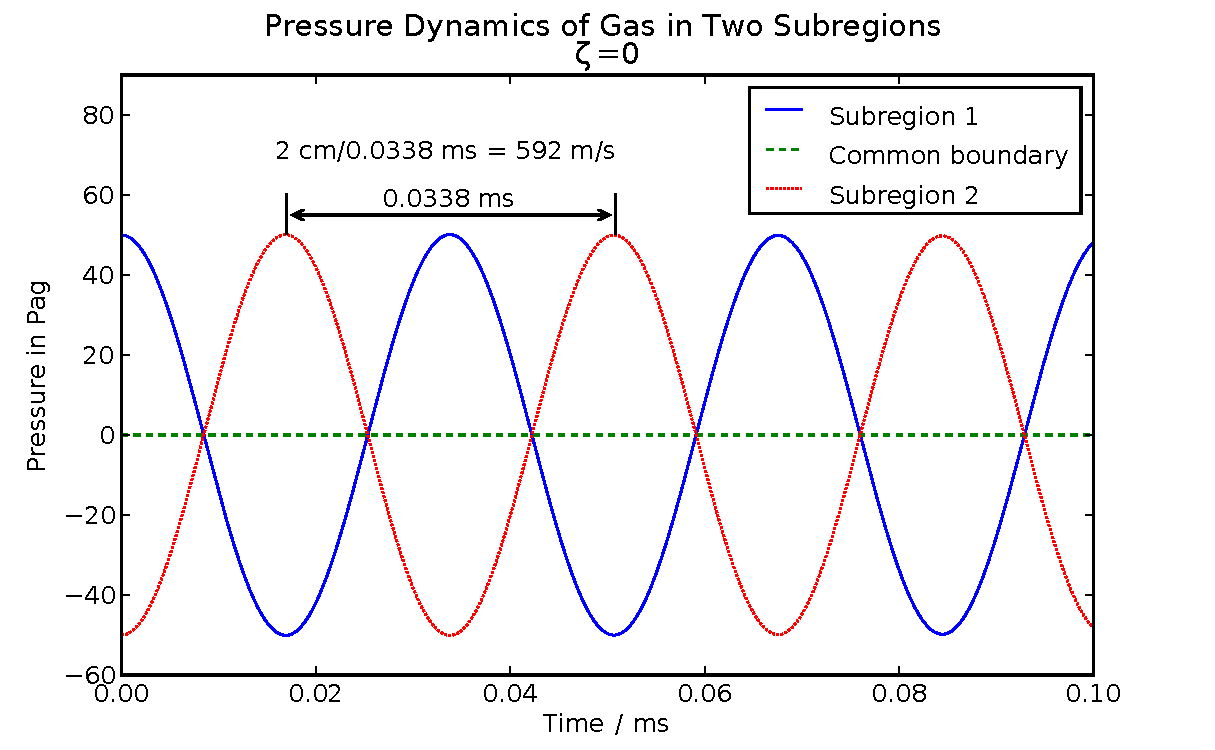
\includegraphics[width=\linewidth]{Results/Basic/Echo/3/Pressure}%
    \label{fig:EchoPressureNoDamping}
  }
  \caption{Pressure dynamics in the echo example}
  \label{fig:EchoPressure}
\end{figure}

Due to thermodynamics, the temperature of the first subregion decreases as its gas expands and the temperature of the second subregion increases as it is compressed.  The changes in temperature are small because the thermal effect is secondary to the main effect of pressure equalization.  As shown in \autoref{fig:EchoTemperature}, the temperature at the common boundary depends on the discretization scheme.  According to upstream discretization, the temperature of the common boundary is biased by the source (\autoref{fig:EchoTemperatureUpstream}).  There is no such bias with the central difference scheme (\autoref{fig:EchoTemperatureCentral}).  Both of these plots are with the default value of continuity ($\s{zeta} = \SI{2.32E-5}{N/A}$).  Since the outer boundaries are adiabatic, the temperature at the outer boundaries are equal to the temperature of the nearest subregion.  At the end of these plots (\SI{0.05}{ms}), the temperatures of the regions are different, yet there is very little thermal convection because the velocities have decayed to nearly zero.  Over a much longer period (\SI{2.5}{s}), the temperatures equalize due to thermal conduction, as shown in \autoref{fig:EchoTemperatureLong}.  The long-term trend of temperature is the same for upstream discretization and the central difference scheme.

\begin{figure}[htbp]
  \subfloat[Upstream discretization]{
    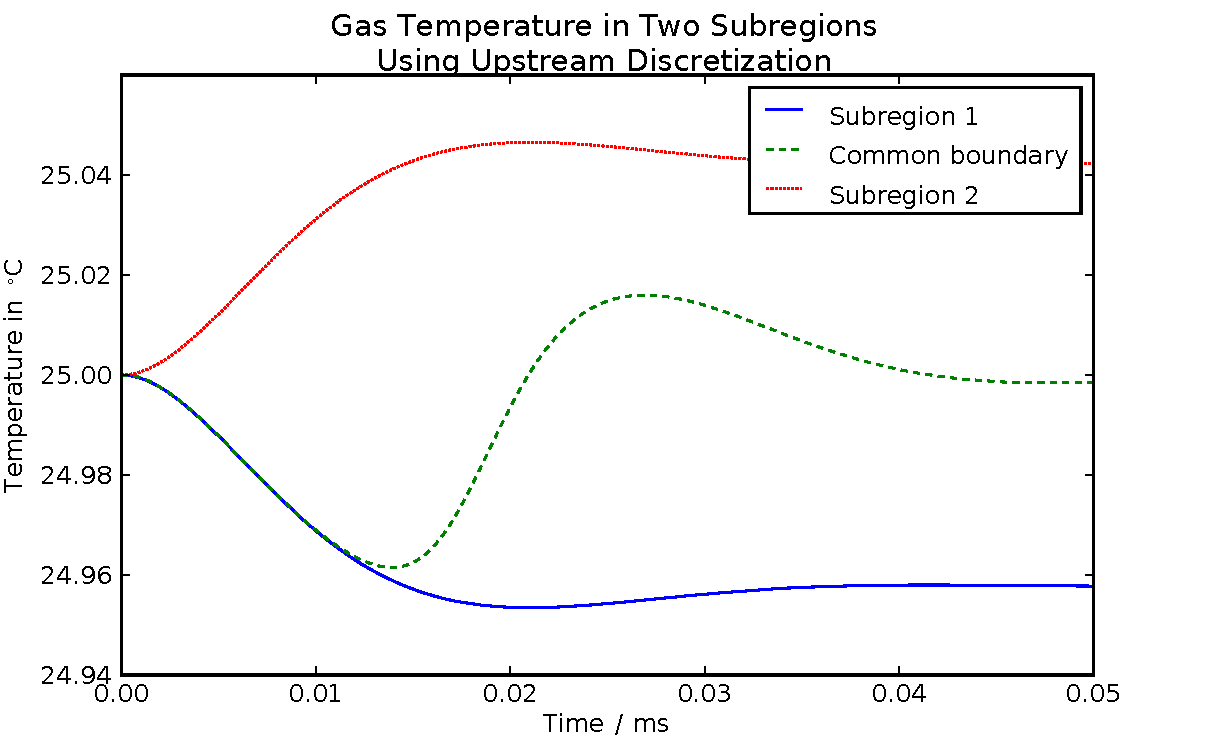
\includegraphics[width=\linewidth]{Results/Basic/Echo/2/Temperature}%
    \label{fig:EchoTemperatureUpstream}
  }\quad
  \subfloat[Central difference scheme]{
    \includegraphics[width=\linewidth]{Results/Basic/Echo/5/Temperature}%
    \label{fig:EchoTemperatureCentral}
  }
  \caption{Temperature oscillations in the echo example}
  \label{fig:EchoTemperature}
\end{figure}

\begin{figure}[htbp]
  \includegraphics[width=\linewidth]{Results/Basic/Echo/1/Temperature}%
  \caption{Long-term thermal equilibration in the echo example}
  \label{fig:EchoTemperatureLong}
\end{figure}

Gas travels in the positive direction due to the initial pressure difference and then returns due to compression, as shown in \autoref{fig:EchoVelocity}.  Although it is not apparent in \autoref{fig:EchoVelocityDampened}, the magnitude of the velocity is slightly greater in the second subregion because that subregion initially has less mass and therefore greater acceleration from a given pressure difference.  This is shown in \autoref{fig:EchoVelocityZoom}.  The plots are for the case of upstream discretization, but the central difference scheme gives identical results.

\begin{figure}[htbp]
  \subfloat[Dampened oscillation]{
    \includegraphics[width=\linewidth]{Results/Basic/Echo/2/Velocity}%
    \label{fig:EchoVelocityDampened}
  }\quad
  \subfloat[Close-up of first crest]{
    \includegraphics[width=\linewidth]{Results/Basic/Echo/2/VelocityZoom}%
    \label{fig:EchoVelocityZoom}
  }
  \caption{Velocity in the echo example}
  \label{fig:EchoVelocity}
\end{figure}


\FloatBarrier % Flush the floats.
\section{Air Column}

This example shows the effect of body forces on a gas.  Like the previous example, it exhibits oscillations due to the coupled dynamics of translation and compression.  The key model equations are material transport (\autoref{eq:MaterialTransport}), material conservation (\autoref{eq:MaterialBalance}), and the translational momentum balance (\autoref{eq:TranslationalBalance}).

\subsection{Conditions}

A vertical column of five \SI{10 x 10 x 10}{m} subregions contain \n{N2} gas (roughly representing air), as shown in \autoref{fig:AirColumn}.  The gas is initialized uniformly to \SI{25}{\celsius} and \SI{1}{bar}.  The external boundaries are isolated (i.e., closed, adiabatic, and free-slip) except for the upper boundary which is held at \SI{25}{\celsius} and \SI{1}{bar}.  Standard gravity is applied (\SI{9.81}{m/s^2}).  The central difference scheme is used.

\begin{figure}[htbp]
  \subfloat[Physical domain]{
    \fbox{\includegraphics[height=4.4in]{5-AirColumn}}%
    \label{fig:AirColumnPhysical}
  }\hspace*{-3.2cm}\includegraphics[height=3.9in]{5-AirColumnLink}\hspace*{-1.3cm}
  \subfloat[Model]{
    \fbox{\includegraphics[height=3.7in]{5-AirColumnD}}%
    \label{fig:AirColumnDiagram}
  }
  \caption{Configuration of the air column example (gas under the influence of gravity)}
  \label{fig:AirColumn}
\end{figure}

\subsection{Results and Discussion}

\begin{contextbox}
  Modeling and simulation statistics:
  \begin{itemize}
    \item Number of variables: 1168
    \item Number of time-varying variables: 284
    \item Number of states: 15
    \item Sizes of the nonlinear systems of equations: None
    \item Sizes of the linear systems of equations: 8 sets of 2
    \item Translation time: \SI{3}{s}
    \item Simulation time: \SI{0.016}{s}
  \end{itemize}
\end{contextbox}

This model has roughly twice as many variables as the previous examples, yet it translates and simulates in about the same time.  There are 15 states---the temperature, pressure, and vertical component of velocity in each of the five subregions.

The total pressure difference over all the subregions is plotted in \autoref{fig:AirColumnPressureDifference}.  It oscillates due to the dynamics of translation and compression.  It takes approximately \SI{3}{s} for the pressure difference to settle to the expected value---the product of density, acceleration due to gravity, and column height ($\s{m}\s{rho}\s{a}[_y]\s{L}[_y]$).  \autoref{fig:AirColumnPressureDistribution} shows that the pressure gradient is uniform at steady state, as expected.

\begin{figure}[htbp]
  \subfloat[Total pressure difference]{
    \includegraphics[width=\linewidth]{Results/Basic/AirColumn/2/PressureDifference}%
    \label{fig:AirColumnPressureDifference}
  }\quad
  \subfloat[Pressure distribution]{
    \includegraphics[width=\linewidth]{Results/Basic/AirColumn/2/Pressure}%
    \label{fig:AirColumnPressureDistribution}
  }
  \caption{Pressure in the air column example}
  \label{fig:AirColumnPressure}
\end{figure}

As shown in \autoref{fig:AirColumnVelocity}, the gas accelerates downward and then rebounds upward due to compression.  The maximum downward velocity is approximately \SI{85}{cm/s} at the upper boundary.

\begin{figure}[htbp]
  \includegraphics[width=\linewidth]{Results/Basic/AirColumn/2/Velocity}%
  \caption{Velocity transients in the air column example}
  \label{fig:AirColumnVelocity}
\end{figure}

The temperatures of the subregions increase due to the adiabatic compression, as shown in \autoref{fig:AirColumnTemperatureShort}.  This develops a temperature gradient where the lower subregions are slightly hotter.  In reality, this would lead to natural convection.  However, in this idealized model, there is only one transport path and no way for a circulation cell to develop.  Therefore, the temperature can only equalize by conduction.\footnote{The model also assumes no thermal radiation.}  The time constants, which are calculated as output variables of the model and plotted in \autoref{fig:AirColumnTimeConstants}, are approximately 19~days for transport from a boundary into a subregion due to the size of the system and the properties of the gas.  These large time constants do in fact match the theoretical result. \autoref{fig:AirColumnTemperatureLong} shows the long-term temperature trends.  The full equalization takes approximately three years.  While this example is rather academic, it demonstrates the stability and flexibility of the model and the solver.  The same translated model was used for both the short- and long-term simulations---a ratio of \num{31557600} in simulated time---with roughly the same computation time (16 and \SI{19}{ms}).

\begin{figure}[htbp]
  \subfloat[Initial oscillations]{
    \includegraphics[width=\linewidth]{Results/Basic/AirColumn/2/Temperature}%
    \label{fig:AirColumnTemperatureShort}
  }\quad
  \subfloat[Equalization over the long term]{
    \includegraphics[width=\linewidth]{Results/Basic/AirColumn/1/Temperature}%
    \label{fig:AirColumnTemperatureLong}
  }
  \caption[Thermal transients in the air column example]{Thermal transients in the air column example.  Since the boundaries are adiabatic, the temperatures of the lower and upper boundaries (not plotted) are equal to the temperatures of subregions 1 and 5}
  \label{fig:AirColumnTemperature}
\end{figure}

\begin{figure}[htbp]
  \includegraphics[width=\linewidth]{Results/Basic/AirColumn/1/TimeConstants}%
  \caption{Thermal time constants in the air column example}
  \label{fig:AirColumnTimeConstants}
\end{figure}


\FloatBarrier % Flush the floats.
\section{Electrical Conduction}

This is an example of Ohm's law with thermal dynamics.  The key equations are translational exchange (\autoref{eq:TranslationalDiffusiveExchange}), thermal conduction (\autoref{eq:ThermalDiffusiveTransport}), and the energy balance (\autoref{eq:EnergyBalanceIntensive}).

\subsection{Conditions}

A $\SI{1}{m}\times\SI{1}{mm}\times\SI{1}{mm}$ block of graphite is held at \SI{25}{\celsius}, as shown in \autoref{fig:ElectricalConduction}.  An electrical current ($\s{z}{I}$) of \SI{50}{mA} is pulled from the negative boundary (\s{e-} into the boundary), and the positive boundary is held at a reference electronic pressure\slash{}potential.  The electrical conductivity (\s{sigma}) is \SI{100}{S/m}.  The perimeter is closed and adiabatic.

\begin{figure}[htbp]
  \subfloat[Physical domain]{
    \fbox{\includegraphics[width=\linewidth]{5-ElectricalConduction}}%
    \label{fig:ElectricalConductionPhysical}
  }\\
   \subfloat[Model]{ 
\fbox{\begin{minipage}{0.5\linewidth}
    \includegraphics[width=\linewidth, clip, trim=0 110 0 0]{5-ElectricalConductionD}\\
    \includegraphics[width=\linewidth, clip, trim=0 0 0 130]{5-ElectricalConductionD}%
\end{minipage}}
    \label{fig:ElectricalConductionDiagram}
  }
  \caption{Configuration of the electrical conduction example}
  \label{fig:ElectricalConduction}
\end{figure}

\subsection{Results and Discussion}

\begin{contextbox}
  Modeling and simulation statistics:
  \begin{itemize}
    \item Number of variables: 374
    \item Number of time-varying variables: 31
    \item Number of states: 1
    \item Sizes of the nonlinear systems of equations: None
    \item Sizes of the linear systems of equations: None
    \item Translation time: \SI{3}{s}
    \item Simulation time: \SI{0.005}{s}
  \end{itemize}
\end{contextbox}

As expected, the simulation shows an electrical resistance of $\s{R} = \s{L}/\s{sigma}\s{A} = \SI{100}{\ohm}$.  The rate of heat generation is $\dot{Q}[_gen] = (\s{z}{I})^2\s{R} = \SI{250}{mW}$.  

\autoref{fig:ElectricalConductionTemperature} shows the temperature trend.  As expected, the steady-state temperature is $\s{T} = \s{T}_0 + \s{theta}\s{L}\dot{Q}[_gen]/4\s{A} \approx \SI{82}{\celsius}$, where $\s{T}_0$ is the boundary temperature (\SI{25}{\celsius}), \s{theta}~is the thermal resistance, \s{L}~is the length (\SI{1}{cm}), and \s{A}~is the cross-sectional area (\SI{1}{mm^2}).  The factor of one fourth is due to the boundary conditions; the conduction length is half of the total length and the heat is rejected to both sides.  The time constant, as measured by the time to $1 - e^{-1} (\approx 63\%$) of the final value, is approximately equal to $\s{tau}\sub{_Q}[_T]/2$, were $\s{tau}\sub{_Q}[_T]$~is the time constant for thermal conduction from one side into the subregion (\autoref{eq:TimeConstantThermalTransport}).

\begin{figure}[htbp]
  \includegraphics[width=\linewidth]{Results/Basic/ElectricalConduction/Temperature}%
  \caption{Dynamic heating of an electrical resistor}%
  \label{fig:ElectricalConductionTemperature}
\end{figure}


\FloatBarrier % Flush the floats.
\section{Thermal Conduction}
\label{sec:ThermalConduction}

This example demonstrates distributed thermal conduction and heating.  The key model equations are thermal conduction (\autoref{eq:ThermalDiffusiveTransport}) and the energy balance (\autoref{eq:EnergyBalanceIntensive}).

\subsection{Conditions}
\label{sec:ThermalConductionConditions}

A graphite bar divided into eight \SI{1}{cm^3} subregions, as shown in \autoref{fig:ThermalConduction}.  The initial temperature of the first subregion is \SI{55}{\celsius}; the others begin at \SI{25}{\celsius}.  The outer boundaries are adiabatic.

\begin{figure}[htbp]
  \subfloat[Physical domain]{
    \fbox{\includegraphics[width=\linewidth]{5-ThermalConduction}}%
    \label{fig:ThermalConductionPhysical}
  }\vspace*{-1.72cm}\\\includegraphics[width=\linewidth]{5-ThermalConductionLink}\vspace*{-1cm}\\
  \subfloat[Model]{
    \fbox{\includegraphics[width=0.6\linewidth]{5-ThermalConductionD}}%
    \label{fig:ThermalConductionDiagram}
  }
  \caption{Configuration of the thermal conduction example}
  \label{fig:ThermalConduction}
\end{figure}

\subsection{Results and Discussion}

\begin{contextbox}
  Modeling and simulation statistics:
  \begin{itemize}
    \item Number of variables: 1119
    \item Number of time-varying variables: 80
    \item Number of states: 8
    \item Sizes of the nonlinear systems of equations: None
    \item Sizes of the linear systems of equations: 7 sets of 2
    \item Translation time: \SI{3}{s}
    \item Simulation time: \SI{0.009}{s}
  \end{itemize}
\end{contextbox}

\autoref{fig:ThermalConductionTemperature} shows the temperature trends throughout the graphite bar.  The temperatures distribute evenly and then converge to a final temperature of approximately \SI{28}{\celsius} after \SI{500}{s}.  Since there is no material transport, the temperatures of the interfaces are the average temperatures of the neighboring subregions.  

\begin{figure}[htbp]
  \includegraphics[width=\linewidth]{Results/Basic/ThermalConduction/Temperature}%
  \caption{Temperature in a graphite bar during transient conduction}%
  \label{fig:ThermalConductionTemperature}
\end{figure}


\FloatBarrier % Flush the floats.
\section{Thermal Conduction and Convection}
\label{sec:ThermalConductionConvection}

This example builds on the previous one.  It adds gas to the system and shows how the gas moves as the temperature equalizes.  Material transport (\autoref{eq:MaterialTransport}) and translational exchange (\autoref{eq:TranslationalDiffusiveExchange}) are important here.

\subsection{Conditions}

The conditions are the same as described in \autoref{sec:ThermalConductionConditions}, except that \n{N2} gas now occupies half of the volume of each subregion.  The gas is initialized to \SI{1}{atm} and the same temperature as the solid.  Initially, it has zero velocity.  The translational independence factor is ten ($\s{k}\sub{_Phi}[_x] = 10$), which represents a porous media.

\begin{figure}[htbp]
  \subfloat[Physical domain]{
    \fbox{\includegraphics[width=\linewidth]{5-ThermalConductionConvection}}%
    \label{fig:ThermalConductionConvectionPhysical}
  }\vspace*{-1.72cm}\\\includegraphics[width=\linewidth]{5-ThermalConductionLink}\vspace*{-1cm}\\
  \subfloat[Model]{
    \fbox{\includegraphics[width=0.6\linewidth]{5-ThermalConductionConvectionD}}%
    \label{fig:ThermalConductionConvectionDiagram}
  }
  \caption{Configuration of the thermal conduction and convection example}
  \label{fig:ThermalConductionConvection}
\end{figure}

\subsection{Results and Discussion}

\begin{contextbox}
  Modeling and simulation statistics:
  \begin{itemize}
    \item Number of variables: 2407
    \item Number of time-varying variables: 574
    \item Number of states: 31
    \item Sizes of the nonlinear systems of equations: None
    \item Sizes of the linear systems of equations: 43 sets of 2
    \item Translation time: \SI{5}{s}
    \item Simulation time: \SI{0.072}{s}
  \end{itemize}
\end{contextbox}

The simulation is approximately eight times slower than the example without the gas (\autoref{sec:ThermalConduction}).  There are states for the temperature of the solid and the temperature and pressure of the gas in every subregion (24 states).  There are also states for the x component of velocity in all but one subregion (7 states).  One of the translational states is eliminated due to the closed outer boundaries.

The temperature trends are nearly the same as for the previous example (\autoref{fig:ThermalConductionTemperature}).  The gas and the solid remain at approximately the same temperature in each subregion.  

Due to the equation of state, the gas in the first subregion becomes denser and has lower pressure as it becomes colder.  This is shown in Figures~\ref{fig:ThermalConductionConvectionVelocity} and \ref{fig:ThermalConductionConvectionPressure}.  The gas in the first two subregions begins to travel very slowly (on the order of \SI{10}{\micro\m/\s}) in the negative direction, into those subregions as they cool.  Due to conservation of momentum, the gas begins to move in the opposite (positive) direction in other regions in the first \SI{100}{s}.  The expansion around the second interface is driven by a higher pressure there.  Shortly after \SI{100}{s}, the pressure in the last subregion reaches a maximum and counters the movement towards the positive outer boundary.

\begin{figure}[htbp]
  \includegraphics[width=\linewidth]{Results/Basic/ThermalConductionConvection/Velocity}%
  \caption{Velocity induced in gas in contact with graphite undergoing thermal conduction}%
  \label{fig:ThermalConductionConvectionVelocity}
\end{figure}

\begin{figure}[htbp]
  \includegraphics[width=\linewidth]{Results/Basic/ThermalConductionConvection/Pressure}%
  \caption{Pressure induced in gas in contact with graphite undergoing thermal conduction}%
  \label{fig:ThermalConductionConvectionPressure}
\end{figure}


\FloatBarrier % Flush the floats.
\section{Evaporation}
\label{sec:Evaporation}

This example demonstrates the evaporation of liquid water into an initially sub-saturated vapor until equilibrium is reached.  The cooling effect of evaporation is evident.  The key equations are the rate of phase change (\autoref{eq:PhaseChange}) and the energy balance (\autoref{eq:EnergyBalanceIntensive}).

\subsection{Conditions}

Water vapor and liquid water are present in a closed, adiabatic volume of \SI{1}{cm^3}.  Initially, 0.1\% of the volume is filled with liquid, and the water is at \SI{25}{\celsius} and \SI{1}{kPa} in both phases.  These conditions are below saturation.  Capillary pressure is considered negligible.

\begin{figure}[htbp]
  \subfloat[Physical domain]{
    \fbox{\includegraphics[width=0.5\linewidth]{5-Evaporation}}%
    \label{fig:EvaporationPhysical}
  }\\
   \subfloat[Model]{ 
\fbox{\begin{minipage}{0.25\linewidth}
    \includegraphics[width=\linewidth, clip, trim=0 140 0 0]{5-EvaporationD}\\
    \includegraphics[width=\linewidth, clip, trim=0 0 0 110]{5-EvaporationD}%
\end{minipage}}
    \label{fig:EvaporationDiagram}
  }
  \caption{Configuration of the evaporation and condensation example}
  \label{fig:Evaporation}
\end{figure}

\subsection{Results and Discussion}

\begin{contextbox}
  Modeling and simulation statistics:
  \begin{itemize}
    \item Number of variables: 537
    \item Number of time-varying variables: 143
    \item Number of states: 5
    \item Sizes of the nonlinear systems of equations: None
    \item Sizes of the linear systems of equations: 3, 2, 2
    \item Translation time: \SI{3}{s}
    \item Simulation time: \SI{0.012}{s}
  \end{itemize}
\end{contextbox}

Some of the liquid evaporates until saturation is reached.  As shown in \autoref{fig:EvaporationPressure}, this takes approximately \SI{2}{ms}.  \autoref{fig:EvaporationRate} shows the rate of evaporation over time.  The temperature is shown in \autoref{fig:EvaporationTemperature}.  It deceases by approximately \SI{43}{mK} due to the latent heat of evaporation.  

\begin{figure}[htbp]
  \includegraphics[width=\linewidth]{Results/Basic/Evaporation/1/Pressure}%
  \caption{Pressure of \s{H2O} reaching saturation}%
  \label{fig:EvaporationPressure}
\end{figure}

\begin{figure}[htbp]
  \includegraphics[width=\linewidth]{Results/Basic/Evaporation/1/Rate}%
  \caption{Rate of evaporation of initially sub-saturated \s{H2O}}%
  \label{fig:EvaporationRate}
\end{figure}

\begin{figure}[htbp]
  \includegraphics[width=\linewidth]{Results/Basic/Evaporation/1/Temperature}%
  \caption{Temperature of \s{H2O} during evaporation}%
  \label{fig:EvaporationTemperature}
\end{figure}

As discussed in \autoref{sec:PhaseChange}, the model uses thermodynamic properties (specific Gibbs energy) to describe phase equilibrium instead of a separate function for saturation pressure.  \autoref{fig:SaturationPressure} compares the equivalent saturation pressure of the model to a saturation pressure function from \modelica{Modelica.Media}.  The model is evaluated as an ideal gas and using the second-order virial coefficients from~\cite{Dymond2002}.  The match is better with the second-order equation of state, but the model has sufficient accuracy with the ideal gas assumption.

\begin{figure}[htbp]
  \includegraphics[width=\linewidth]{Results/Basic/Evaporation/2/SaturationPressure}%
  \caption{Validation of~\s{H2O} saturation pressure}%
  \label{fig:SaturationPressure}
\end{figure}


\FloatBarrier % Flush the floats.
\section{Hydration}
\label{sec:Hydration}

This example is similar to the previous one, but the phase change is between the liquid and ionomer instead of between the liquid and gas. 

\subsection{Conditions}

Liquid and hydrated ionomer each occupy 30\% of a cubic \SI{1}{cm^3} control volume, as shown in \autoref{fig:Hydration}.  No water enters or exits.  An inert gas (\s{N2}) fills the rest of the volume at \SI{1}{atm} (fixed).  In order to isolate the hydration, it is assumed that no evaporation takes place.  The phase change interval (\s{tau}[^prime]) is set to represent a case where the phases are interspersed with a relatively large amount of contact.  All of the materials are held at \SI{60}{\celsius}.  The ionomer is initialized with a hydration level of $\s{lambda} = 8$, where \s{lambda}~is the number of \s{H2O} molecules divided by the number of \s{SO3-} end groups.  This is below the equilibrium level of hydration.

\begin{figure}[htbp]
  \subfloat[Physical domain]{
    \fbox{\includegraphics[width=0.5\linewidth]{5-Hydration}}%
    \label{fig:HydrationPhysical}
  }\\
   \subfloat[Model]{ 
\fbox{\begin{minipage}{0.25\linewidth}
    \includegraphics[width=\linewidth, clip, trim=0 140 0 0]{5-HydrationD}\\
    \includegraphics[width=\linewidth, clip, trim=0 0 0 110]{5-HydrationD}%
\end{minipage}}
    \label{fig:HydrationDiagram}
  }
  \caption{Configuration of the hydration example}
  \label{fig:Hydration}
\end{figure}

\subsection{Results and Discussion}

\begin{contextbox}
  Modeling and simulation statistics:
  \begin{itemize}
    \item Number of variables: 654
    \item Number of time-varying variables: 68
    \item Number of states: 1
    \item Sizes of the nonlinear systems of equations: None
    \item Sizes of the linear systems of equations: 3 sets of 2
    \item Translation time: \SI{3}{s}
    \item Simulation time: \SI{0.011}{s}
  \end{itemize}
\end{contextbox}

Water is absorbed until the hydration level is in equilibrium with the liquid.  This takes approximately two minutes, as shown in \autoref{fig:EvaporationPressure}.  \autoref{fig:HydrationRate} shows the rate of absorption over time.  

\begin{figure}[htbp]
  \includegraphics[width=\linewidth]{Results/Basic/Hydration/1/Level}%
  \caption{Hydration level of the ionomer reaching equilibrium}%
  \label{fig:HydrationLevel}
\end{figure}

\begin{figure}[htbp]
  \includegraphics[width=\linewidth]{Results/Basic/Hydration/1/Rate}%
  \caption{Rate of hydration of the ionomer}%
  \label{fig:HydrationRate}
\end{figure}

The model uses thermodynamic properties (specific Gibbs energy) to describe phase equilibrium instead of a separate function for the equilibrium hydration level.  \autoref{fig:HydrationEquil} compares the equivalent equilibrium hydration of the model at \SI{30}{\celsius} to the explicit correlated function from Springer et al.~\cite{Springer1991}.   As given by the implementation (\autoref{sec:Characteristics}), the model matches the correlation of Springer et al.~\cite{Springer1991} at 0 and 100\%.  Between these points, the relationship between relative humidity and hydration is linear and does not match the published correlation.

\begin{figure}[htbp]
  \includegraphics[width=\linewidth]{Results/Basic/Hydration/2/Level}%
  \caption{Equilibrium hydration level versus relative humidity}%
  \label{fig:HydrationEquil}
\end{figure}



\section{Summary}

This chapter provided a wide array of basic examples of the model library.  It is significant that all of the examples were built from the same model elements.  They simulate quickly (${\leq \SI{72}{ms}}$; maximum in \autoref{sec:ThermalConductionConvection}), and there are no nonlinear systems of equations.  The settings of the phase change intervals in Sections~\ref{sec:Evaporation} and ~\ref{sec:Hydration} are the same as those used in the fuel cell model.  The next chapter will address the fuel cell model.


  \chapter{Simulation of the Fuel Cell Model}
  \label{chap:Cell}
  \glsresetall

% Don't show subsections in the TOC.
\addtocontents{toc}{\protect\setcounter{tocdepth}{1}}


This chapter presents the results of the fuel cell model.  The first section investigates the operation of the cell during a baseline polarization test.  The next six sections vary certain properties, such as temperature and pressure, and observe the effects on the polarization curve.  Then, Sections~\ref{sec:SimpleCell} and~\ref{sec:SegCell} show variations of the cell model, specifically a simplified model and a model with multiple segments down the length of the channel.  The final section (\ref{sec:Cycle}) shows the dynamics of the model under a cyclical load.  All of the results are from the fuel cell model except for the experimental data used in Figures~\ref{fig:BaselinePolarization} and \ref{fig:TemperaturePolarization} through \ref{fig:CaHumidityPolarization} to benchmark the model.


\section{Baseline Polarization Test}
\label{sec:Baseline}

\subsection{Test Conditions}
\label{sec:Baseline-Conditions}

The \modelica{TestStand} model presented in \autoref{sec:TestStand} applies boundary conditions to the \modelica{Cell} model.  Under the baseline conditions, the temperature of the reactant supplies and the exterior x-axis boundary of the flow plates is \SI{60}{\celsius}.  This temperature is used to initialize the layers as well.  Both outlets are maintained at \SI{48.3}{kPag}.  The cell operates on \s{H2} humidified to 80\% and air humidified to 50\%.  The reactant supply varies stoichiometrically according to the electrical load.  The stoichiometric ratio is 1.5 in the anode and 2.0 in the cathode.  After an initial three minutes to reach steady conditions at \SI{0.1}{mA}, the electrical load is ramped at a rate of \SI{0.3}{A/cm^2} per hour for ten hours or until the cathode is depleted of \s{O2}.  A slow ramp rate is used so that the dynamic effects are negligible.  Although the model has options to assume steady state conditions, the states are generally necessary to avoid nonlinear systems of equations.

The area of the cell is \SI{50}{cm^2}.  There is one subregion for each layer.  Ideal gases are assumed.  Liquid is included.  The double layer capacitances are not included in order to eliminate some of the dynamics.  The key physical parameters of the model are listed in \autoref{tab:CellParams}.  The values roughly correspond to a test cell used at the \n{HNEI} to provide the benchmark data, which is shown in the results.  Where possible, the values are cited and justified in the model documentation (\autoref{chap:Doc}).  Due to the complexity of the model and the limitations of physical sensors, it is not possible to directly establish some of the parameters, especially those that deal with transfer rates.  This is a known issue with fuel cell models in general~\cite{Faghri2005}.  

Other parameters are listed in the tables of \autoref{chap:Doc}.  The thermodynamic correlations from McBride et al.~\cite{McBride2002} are used for the fluids.  The fluidity and thermal resistivities are based on the correlations from Svehla et al.~\cite{Svehla1995} and tables from Incropera and DeWitt~\cite{Incropera2002}.  The kinetic theory of gases~\cite{Present1958} is used to approximate properties that are not available directly.  

%The geometries of the cell's flow plates were established by General Motors with serpentine flow fields of two parallel anode channels and three parallel cathode channels.  The \n{MEA} was produced by Ion Power~\cite{IonPower2009} and the \np{GDL} are model 25BC from SGL~\cite{SGL2004}.  The cell was operated under stoichiometrically varying reactant flows on a test stand from Greenlight Innovation at the \n{HNEI}.  

\begin{sidewaystable}[hbtp]
  \caption{Key parameters of the fuel cell model}
  \label{tab:CellParams}
  \begin{tabular}{llllllll}
    \toprule
     & \textbf{anFP} & \textbf{anGDL} & \textbf{anCL} & \textbf{PEM} & \textbf{caCL} & \textbf{caGDL} & \textbf{caFP} \\
    \midrule
    Volumetric porosity & 0.059 & 0.8 & 0.4 & --- & 0.4 & 0.8 & 0.042 \\
    Thickness / mm & 10 & 0.235 & 0.029 & 0.04 & 0.029 & 0.235 & 10 \\
    Channel length / m & 1.62 & --- & --- & --- & --- & --- & 1.06 \\
    Hydraulic diameter / \SI{}{mm^2} & 0.94 & --- & --- & --- & --- & --- & 0.82 \\
    Electronic conductivity / \SI{}{S.cm^{-1}} & 680 & 3.3\footnote{\label{note1}This is for the bulk media (i.e., after accounting for porosity).} & 3.3\footnoteref{note1} & --- & 3.3\footnoteref{note1} & 3.3\footnoteref{note1} & 680 \\
    Protonic conductivity\footnote{This only describes coupling with the solid.  Electro-osmotic drag (coupling with \s{H2O}) introduces additional resistance.} / \SI{}{S.cm^{-1}} & --- & --- & 0.1 & 0.1 & 0.1 & --- & --- \\
    Thermal resistivity of carbon / \SI{}{m.K.W^{-1}} & 0.01 & 0.85\footnoteref{note1} & 0.85\footnoteref{note1} & --- & 0.85\footnoteref{note1} & 0.85\footnoteref{note1} & 0.01 \\
    Thermal resistivity of dry ionomer / \SI{}{m.K.W^{-1}} & --- & --- & 6.25 & 6.25 & 6.25 & --- & --- \\
    Exchange current density @ \SI{300}{K} / \SI{}{A.cm^{-2}} & --- & --- & 1 & --- & \num{2.3E-5} & --- & --- \\
    Activation energy / V & --- & --- & 0 & --- & 0.75 & --- & --- \\
    Contact angle & \SI{90}{\degree} & \SI{140}{\degree} & \SI{140}{\degree} & --- & \SI{140}{\degree} & \SI{140}{\degree} & \SI{90}{\degree} \\
    Effective pore radius / \SI{}{\micro.m} & --- & 32 & 5 & --- & 5 & 32 & --- \\
    Evaporation interval / ms & 16 & 16 & 16 & --- & 16 & 16 & 16 \\
    Absorption interval / s & --- & --- & 33 & --- & 33 & --- & --- \\
    Common mobility factor & \num{E7}\footnote{\label{note2}This is in the x direction (through the cell).  In the y direction (down the channel), it is infinite.} & 1.7 & 1.7 & $\infty$ & 1.7 & 1.7 & \num{E7}\footnoteref{note2} \\
    Mobility factor between gas and liquid & \num{E6}\footnoteref{note2} & $\infty$ & $\infty$ & --- & $\infty$ & $\infty$ & \num{E6}\footnoteref{note2} \\
    Mobility factor between \s{H+} and \s{H2O} & --- & --- & 0.02 & 0.02 & 0.02 & --- & --- \\
    Mobility factor between \s{H2O} and \s{SO3-} & --- & --- & 1 & 1 & 1 & --- & --- \\
    Common thermal independence factor & \num{E5} & 0 & 0 & 0 & 0 & 0 & \num{E5} \\
    \bottomrule
  \end{tabular}
\end{sidewaystable}


\subsection{Results and Discussion}
\label{sec:Baseline-Results}

\begin{contextbox}
  Modeling and simulation statistics:
  \begin{itemize}
    \item Number of variables: 6887
    \item Number of time-varying variables: 2749
    \item Number of states: 55
    \item Sizes of the nonlinear systems of equations: None
    \item Sizes of the linear systems of equations: 1 set of 9, 1 set of 8, 1 set of 6, 2 sets of 5, 9 sets of 4, 18 sets of 3, 97 sets of 2
    \item Translation time: \SI{23}{s}
    \item Simulation time: \SI{1.56}{s}
  \end{itemize}
\end{contextbox}

The cell model is much more complex than the models of \autoref{chap:Basic}, but as indicated by the simulation time of under two seconds, the translator and solver handle it well.  There are no nonlinear systems of equations.  The 55 states of the model include the following temperatures:
\begin{enumerate*}
  \item anFP gas
  \item anFP liquid
  \item anFP solid (graphite)
  \item anGDL (all phases combined)
  \item anCL (all phases combined)
  \item PEM
  \item caCL (all phases combined)
  \item anGDL (all phases combined)
  \item caFP gas
  \item caFP liquid
  \item caFP solid (graphite)
\end{enumerate*}
It is assumed that all of the species have the same temperature in the interior layers, regardless of phase, because the associated time constants were calculated by the model to be very quick (between \num{E-11} and \SI{E-7}{s}).  The following 24 amounts of material also appear as states:
\begin{enumerate*}
  \item \s{H2} in the anFP, anGDL, and anCL (3)
  \item \s{H2O} as gas in the anFP, anGDL, anCL, caCL, caGDL, and caFP (6)
  \item \s{H2O} as liquid in the anFP, anGDL, anCL, caCL, caGDL, and caFP (6)
  \item \s{H2O} in the ionomer of the anCL, PEM, and caCL (3)
  \item \s{N2} in the caCL, caGDL, and caFP (3)
  \item \s{O2} in the caCL, caGDL, and caFP (3)
\end{enumerate*}
There are 14 states related to velocity:
\begin{enumerate*}
  \item x-direction velocity of \s{H2} in the anGDL and anCL (2)
  \item x-direction velocity of \s{H2O} gas in the anGDL, caCL, and caGDL (3)
  \item x-direction velocity of \s{H2O} liquid in the anGDL, anCL, caCL, and caGDL (4)
  \item y-direction velocity of \s{H2O} liquid in the anFP and caFP (2)
  \item x-direction velocity of \s{H2O} in the ionomer of the anCL and caCL (2)
  \item x-direction velocity of \s{N2} in the caGDL (1)
\end{enumerate*}
The y-direction velocities are constrained by the boundary conditions, so they are not independent for each species.  The final group of states contains these currents:
\begin{enumerate*}
  \item x- and y-direction currents of \n{H2O} gas in the anFP (2)
  \item x-direction current of \n{O2} in the caCL and caGDL (2)
  \item x- and y-direction currents of \n{N2} in the caFP (2)
\end{enumerate*}
For numerical reasons, it is sometimes better to choose currents as states instead of velocities.

\autoref{fig:BaselinePolarization} compares the polarization of the cell model against seven runs of the experimental cell over the span of about a week.  There are significant differences.  At the lowest current measured by experiment (\SI{0.1}{A/cm^2}), the model overpredicts the voltage.  This may be due to the \n{H2} crossover current, which was significant in the experimental cell but not included in the model.  The modeling framework could be used to include this phenomena, but that development is left as future work.  At mid-range current, the model underpredicts the voltage.  This is a consequence of tuning the exchange current density to compromise between the low and mid-range current given the fact that \n{H2} crossover is not included.  At higher currents, the voltage of the experimental cell drops---probably due to the effect of liquid water on the concentration\slash{}transport losses.  Although liquid is included in the model and begins to fill the pores of the cathode \n{GDL} as will be shown, it does not have a significant effect on the polarization.

\begin{figure}[htbp]
  \includegraphics[width=\linewidth]{Results/Cell/Model/Baseline/Polarization}%
  \caption{Polarization curves of the cell for the baseline polarization}%
  \label{fig:BaselinePolarization}
\end{figure}

\autoref{fig:BaselineWater} contains a Sankey diagram of the energy balance on the cell at \SI{1.5}{A/cm^2}.  It should be noted that the Sankey diagram indicates the direction of transfer of the quantity (here, energy), not necessarily the direction of material transfer.  In \autoref{fig:BaselineWater}, the inlet and outlet of each stream is combined.  While this helps to show the net rate of contribution, it may be confusing in the case of water.  Since the enthalpy of formation of water is negative by convention, an inflow of water appears as an outflow of energy and vice versa.

The thermodynamic efficiency is only 36\% at this rather high current of \SI{1.5}{A/cm^2}.
% 38.6/(38.6 + 14.3 + 54.3) = 36%
The fact that the main trunk of the Sankey diagram has uniform  thickness indicates that there is no transient energy storage (and the model equations are consistent).  If the load is ramped quickly during a polarization test (e.g., in \autoref{sec:Cycle}), then the energy balance includes significant transients.  These would appear as a taper in the thickness of the trunk between the inputs and outputs.

\begin{figure}[htbp]
  \includegraphics[width=\linewidth]{Results/Cell/Model/1/Energy}%
  \caption{Energy balance under the baseline conditions at \SI{1.5}{A/cm^2}}%
  \label{fig:BaselineEnergy}
\end{figure}

\autoref{fig:BaselineVoltages} shows the losses in the cell.  As expected, the cathode overpotential is dominate.  The next most significant loss is protonic conduction through the catalyst layers and the \n{PEM}.  The anode operates in the regime where the overpotential is linear, in contrast to the Tafel or logarithmic\slash{}exponential regime of the cathode.  The loss due to \n{O2} transport, while small in scale, does begin to increase exponentially near the limiting current density.

\begin{figure}[htbp]
  \includegraphics[width=\linewidth]{Results/Cell/Model/1/PotentialLosses}%
  \caption{Potential losses through the cell during the baseline polarization}%
  \label{fig:BaselineVoltages}
\end{figure}

\autoref{fig:BaselineElectricalLosses} gives information about location of the Ohmic losses, which were grouped as electronic and protonic in \autoref{fig:BaselineVoltages}.  The loss in the \n{PEM}, which is protonic, is the most significant.  The catalyst layers also have large losses, which are a combination of electronic and protonic.  The resistance in the \np{GDL} and flow plates is relatively small.

\begin{figure}[htbp]
  \includegraphics[width=\linewidth]{Results/Cell/Model/1/ElectricalLosses}%
  \caption{Electrical losses in the cell during the baseline polarization}%
  \label{fig:BaselineElectricalLosses}
\end{figure}

The losses generate heat and increase the temperature of the interior of the cell as shown in \autoref{fig:BaselineTemperature}.  The hottest region is the cathode catalyst layer due to the large activation overpotential.  The neighboring regions---the cathode \n{GDL} and the \n{PEM}---have the next highest temperatures.  The cathode is generally hotter than the anode.  More heat is rejected through the cathode flow plate, as was evident in \autoref{fig:BaselineEnergy}.

\begin{figure}[htbp]
  \includegraphics[width=\linewidth]{Results/Cell/Model/1/Temperature}%
  \caption{Temperatures through the cell during the baseline polarization}%
  \label{fig:BaselineTemperature}
\end{figure}

\autoref{fig:PressureGas} shows the pressure of the gas throughout the cell.  It is highest in the cathode flow plate, as this is required to transport \n{O2} into the cell.  Above \SI{2}{A/cm^2}, the pressure of the cathode gas begins to decrease as the concentration limit is reached.  The pressures of the anode are very close to the outlet pressure of \SI{48.3}{kPag}.   \autoref{fig:ChannelPressureDrop} shows the pressure loss along the channels.  The pressure difference between the cathode inlet and outlet is much greater (a factor of nearly 20) than the difference between the anode inlet and outlet.  This is due to the higher viscosity of air relative to \n{H2} and the higher velocity required to deliver \n{O2} since it is at lower concentration in the cathode than \n{H2} is in the anode.

\begin{figure}[htbp]
  \includegraphics[width=\linewidth]{Results/Cell/Model/1/PressureGas}%
  \caption{Total pressure of the gas during the baseline polarization}%
  \label{fig:PressureGas}
\end{figure}

\begin{figure}[htbp]
  \includegraphics[width=\linewidth]{Results/Cell/Model/1/ChannelPressureDrop}%
  \caption{Pressure drop down the flow channels during the baseline polarization}%
  \label{fig:ChannelPressureDrop}
\end{figure}

\autoref{fig:BaselineVelocity} shows the flow through the channels as indicated by the velocity of \n{H2O}.  The velocity is approximately five times higher in the cathode.  In both channels, the velocity of the gas is much higher than the velocity of the liquid.  The gas drags the liquid, yet the liquid has higher viscosity.

\begin{figure}[htbp]
  \includegraphics[width=\linewidth]{Results/Cell/Model/1/Velocity}%
  \caption{Velocity of \s{H2O} down the channels during the baseline polarization}%
  \label{fig:BaselineVelocity}
\end{figure}

The model also includes the pressures of individual gas species.  Figures~\ref{fig:PressureH2}, \ref{fig:PressureH2O}, and \ref{fig:PressureO2} show the pressures of \n{H2}, \n{O2}, and \n{H2O} along their primary transport paths.  The pressure of \n{H2} decreases from the anode inlet to the \n{HOR} and the pressure of \n{O2} decreases from the cathode inlet to the \n{ORR}.  The pressure of \n{H2O} drops from the \n{ORR} to the cathode outlet.

\begin{figure}[htbp]
  \includegraphics[width=\linewidth]{Results/Cell/Model/1/PressureH2}%
  \caption{\s{H2} pressure during the baseline polarization}%
  \label{fig:PressureH2}
\end{figure}

\begin{figure}[htbp]
  \includegraphics[width=\linewidth]{Results/Cell/Model/1/PressureO2}%
  \caption{\s{O2} pressure during the baseline polarization}%
  \label{fig:PressureO2}
\end{figure}

\begin{figure}[htbp]
  \includegraphics[width=\linewidth]{Results/Cell/Model/1/PressureH2O}%
  \caption{\s{H2O} pressure during the baseline polarization}%
  \label{fig:PressureH2O}
\end{figure}

Not all of the \n{H2O} exits from the cathode.  The Sankey diagram in \autoref{fig:BaselineWater} shows the water balance at \SI{1.5}{A/cm^2}.  Water is generated at the rate of \SI{37.5}{A/cm^2} ($\SI{1.5}{A/cm^2} \s{e-} \times \SI{50}{cm^2} \times 1 \s{H2O} / 2 \s{e-}$).  There is a net input of water vapor into the anode and a net output of liquid.  Water exits the cathode channels as gas and liquid.

\begin{figure}[htbp]
  \includegraphics[width=\linewidth]{Results/Cell/Model/1/Water}%
  \caption{\s{H2O} balance under the baseline conditions at \SI{1.5}{A/cm^2}}%
  \label{fig:BaselineWater}
\end{figure}

\autoref{fig:H2OTransport} shows the transport of water through the layers.  It condenses near the interface of the anode flow plate and the anode \n{GDL} because it is super-saturated in the \n{GDL} relative to the channel due to the \n{GDL}'s hydrophobicity.  The current of water through the ionomer is relatively small, but as shown in \autoref{fig:H2OTransportPEM}, it is not zero.  At low currents ($<\SI{1}{A/cm^2}$), there is a fairly linear increase in the rate of transport through the \n{PEM} from the anode to the cathode due to the concentration gradient generated by the production of water in the cathode.  However, the electro-osmotic drag becomes significant at high electrical currents and counters the diffusion.  At the limiting current density, there is a rapid reversal of the trend caused by electro-osmotic drag because the cathode fills with liquid.

\begin{figure}[htbp]
  \includegraphics[width=\linewidth]{Results/Cell/Model/1/H2OTransport}%
  \caption{\s{H2O} transport during the baseline polarization}%
  \label{fig:H2OTransport}
\end{figure}

\begin{figure}[htbp]
  \includegraphics[width=\linewidth]{Results/Cell/Model/1/H2OTransportPEM}%
  \caption[\s{H2O} transport through the membrane during the baseline polarization]{\s{H2O} transport through the \n{PEM} during the baseline polarization}%
  \label{fig:H2OTransportPEM}
\end{figure}

\autoref{fig:BaselineHydration} shows the level of hydration in the ionomer of the catalyst layers and the \n{PEM}.  As the electrical current increases, water is produced more rapidly.  This increases the hydration, beginning in the cathode catalyst layer.  Although the concentration gradient is larger at higher electrical currents, so is the drag due to protonic transport.  As was seen in \autoref{fig:H2OTransportPEM}, the diffusion reaches a maximum (in magnitude) around \SI{1.3}{A/cm^2}.

\begin{figure}[htbp]
  \includegraphics[width=\linewidth]{Results/Cell/Model/1/Hydration}%
  \caption[Hydration during the baseline polarization test]{Hydration of the \n{MEA} during the baseline polarization}%
  \label{fig:BaselineHydration}
\end{figure}

Besides entering the membrane, water also fills the pores of the cathode catalyst layer and \n{GDL}.  This is shown in \autoref{fig:PoreSaturation}.  At the limiting current density, the \n{GDL} pores are 45\% filled and rapidly filling further.  The catalyst layer retains water to a lesser extent.  The model assumes that the pores are smaller in the catalyst layer than the \n{GDL} (see \autoref{tab:CellParams}) but have the same hydrophobicity.  This yields a stronger capillary pressure, which tends to prevent flooding in the catalyst layer.

\begin{figure}[htbp]
  \includegraphics[width=\linewidth]{Results/Cell/Model/1/PoreSaturation}%
  \caption{Liquid pore saturation during the baseline polarization}%
  \label{fig:PoreSaturation}
\end{figure}

\autoref{fig:BaselineRH} shows the humidity throughout the cell.  The relative humidity is slightly higher than 100\% in the cathode channel because the water enters the channel from the catalyst layer and the \n{GDL}, which are hotter due to heat generation.  Also, the \n{GDL}  is modeled as hydrophobic, which implies a lower saturation pressure (i.e., the Kelvin equation) such that saturated vapor in the \n{GDL} is supersaturated in the channel (even at the same temperature).  The vapor in the anode flow plate is saturated, but it appears slightly below 100\% relative humidity.  The reason is that the relative humidity is only an output\slash{}analysis variable in the model.  It is calculated from \modelica{Modelica.Media.Air.MoistAir.saturationPressure()}, which does not correspond exactly to the model.  This was apparent in \autoref{fig:SaturationPressure}.

\begin{figure}[htbp]
  \includegraphics[width=\linewidth]{Results/Cell/Model/1/Humidity}%
  \caption{Relative humidity through the cell during the baseline polarization}%
  \label{fig:BaselineRH}
\end{figure}

\autoref{fig:EvaporationRateCell} shows the rates of evaporation throughout the cell.  Water evaporates most rapidly in the cathode catalyst layer.  The \n{ORR} is modeled as producing liquid, not vapor, and the liquid evaporates to reach saturation.  Water condenses in the other layers.  The largest rate is in the cathode channel.

\begin{figure}[htbp]
  \includegraphics[width=\linewidth]{Results/Cell/Model/1/EvaporationRate}%
  \caption{Rates of evaporation during the baseline polarization}%
  \label{fig:EvaporationRateCell}
\end{figure}

\autoref{fig:CellHydrationRate} shows the rates of hydration in the catalyst layers.  Water is absorbed on the cathode side and desorbed on the anode side where the relative humidity is lower (see \autoref{fig:BaselineRH}) and there is evaporation (see \autoref{fig:EvaporationRateCell}).  Note, however, that the rate of hydration is much slower than the rate of evaporation.  This is consistent with the examples in the last two sections of \autoref{chap:Basic}.

\begin{figure}[htbp]
  \includegraphics[width=\linewidth]{Results/Cell/Model/1/HydrationRate}%
  \caption{Rates of hydration during the baseline polarization}%
  \label{fig:CellHydrationRate}
\end{figure}


\FloatBarrier % Flush the floats.
\section{Varying Temperature}
\label{sec:Temperature}

\subsection{Conditions}

The temperature of the polarization test is changed to 40 and \SI{80}{\celsius} from the 
baseline of \SI{60}{\celsius}.  As mentioned in \autoref{sec:Baseline-Conditions}, the selected temperature is applied to the reactant supples, the exterior x-axis boundaries of the flow plates, and the initial conditions of the cell.  All other settings are the same as for the baseline test (previous section).

\subsection{Results and Discussion}

The model statistics (numbers of both types of variables, number of states, and number of systems of equations) are the same as for the baseline test and the computation times are nearly the same.  Unfortunately, the modeling tool requires that the model be re-translated when the temperature condition is changed.  Sometimes this is necessary when a parameter has implications that may affect the structure of the underlying equations.

\autoref{fig:TemperaturePolarization} compares the polarization of the model against the experimental data.  The same issues are apparent as in \autoref{sec:Baseline-Results}: the model over-predicts the activation region, under-predicts the Ohmic region, and does not show a gradual enough roll-off in the concentration region.  The model does capture the trend towards higher performance at higher temperatures, but not to the extent of the experimental cell.

\begin{figure}[htbp]
  \includegraphics[width=\linewidth]{Results/Cell/Model/Temperature/Polarization}%
  \caption{Polarization curves with varying temperature}%
  \label{fig:TemperaturePolarization}
\end{figure}



\FloatBarrier % Flush the floats.
\section{Varying Pressure}

\subsection{Conditions}

The pressure of the polarization test is changed to 0 and \SI{202.7}{kPag} from the 
baseline of \SI{48.3}{kPag}.  The selected pressure is applied to both of the outlets and to the initial conditions.  All other settings are the same as for the baseline test (\autoref{sec:Baseline}).

\subsection{Results and Discussion}

The model statistics are the same as for the baseline test and the computation times are nearly the same.  Unfortunately, the modeling tool requires that the model be re-translated when the pressure is changed.

\autoref{fig:PressurePolarization} compares the polarization of the model against the experimental data.  The same general issues exist as before.  The model does capture the trend towards higher performance at higher pressure, but not to the extent of the experimental cell.

\begin{figure}[htbp]
  \includegraphics[width=\linewidth]{Results/Cell/Model/Pressure/Polarization}%
  \caption{Polarization curves with varying outlet pressure}%
  \label{fig:PressurePolarization}
\end{figure}


\FloatBarrier % Flush the floats.
\section{Varying Anode Flow Rate}

\subsection{Conditions}

The anode stoichiometric flow rate of the polarization test is changed to 1.1 and 2.0 from the 
baseline of 1.5.  All other settings are the same as for the baseline test (\autoref{sec:Baseline}).

\subsection{Results and Discussion}

The model statistics and translation time are the same as for the baseline test.  The simulation time is only slightly different.  It is possible to change the anode flow rate without re-translating the model.

\autoref{fig:AnFlowPolarization} compares the polarization of the model against the experimental data.  Although the same general issues exist as noted in \autoref{sec:Temperature}, the model and the experimental data both indicate that anode flow rate has little effect on the polarization.  The supply of hydrogen generally does not limit the operation of the cell.  The cathode supply does.

\begin{figure}[htbp]
  \includegraphics[width=\linewidth]{Results/Cell/Model/AnFlow/Polarization}%
  \caption{Polarization curves with varying anode flow rates}%
  \label{fig:AnFlowPolarization}
\end{figure}


\FloatBarrier % Flush the floats.
\section{Varying Cathode Flow Conditions}

\subsection{Conditions}

The cathode stoichiometric flow rate of the polarization test is changed to 1.5 and 2.5 from the 
baseline of 2.0.  In addition, the supply is changed to \s{O2} (no \n{N2}) and the cell is operated at cathode stoichiometric flow rates of 7.177, 9.569, and 11.962.  All other settings are the same as for the baseline test (\autoref{sec:Baseline}).

\subsection{Results and Discussion}

The model statistics and translation time are the same as for the baseline test.  The simulation time is nearly the same.  It is possible to change the cathode flow rate without re-translating the model.  However, the choice of air or \n{O2} requires re-translation.

\autoref{fig:CaFlowPolarization} compares the polarization of the model against the experimental data.  In the case of air (\autoref{fig:CaFlowPolarizationAir}), the effect shown by the model is much less than the effect in the experimental data.  The model is affected very little in the Ohmic region, but the limiting current density changes considerably.  In the case of \s{O2} (\autoref{fig:CaFlowPolarizationO2}), the resistance should decrease significantly in the Ohmic region, but the model does not show it.  As was shown in Figures~\ref{fig:BaselineVoltages} and \ref{fig:BaselineElectricalLosses}, the resistance is dominated by protonic transport through the \n{PEM}.  The protonic resistance does not appear to change in the model.  The only way for it to change is for \begin{inparaenum}[(1)]\item the mobility factors to change (they are currently fixed) or \item the hydration of the \n{PEM} to change, affecting the degree of electro-osmotic drag.\end{inparaenum}

\begin{figure}[htbp]
  \subfloat[Air]{
    \includegraphics[width=\linewidth]{Results/Cell/Model/CaFlowAir/Polarization}%
    \label{fig:CaFlowPolarizationAir}
  }\quad
  \subfloat[Oxygen]{
    \includegraphics[width=\linewidth]{Results/Cell/Model/CaFlowO2/Polarization}%
    \label{fig:CaFlowPolarizationO2}
  }
  \caption{Polarization curves with varying cathode flow rates and compositions}%
  \label{fig:CaFlowPolarization}
\end{figure}


\FloatBarrier % Flush the floats.
\section{Varying Anode Humidity}

\subsection{Conditions}

The relative humidity of the anode supply is changed to 60 and 100\% from the 
baseline of 80\%.  All other settings are the same as for the baseline polarization test (\autoref{sec:Baseline}).

\subsection{Results and Discussion}

The model statistics are the same as for the baseline test and the computation times are nearly the same.  The modeling tool requires that the model be re-translated when the humidity of the anode supply is changed.  

The anode humidity has little effect on the polarization, as shown in \autoref{fig:AnHumidityPolarization} for both the model and the experimental cell.

\begin{figure}[htbp]
  \includegraphics[width=\linewidth]{Results/Cell/Model/AnHumidity/Polarization}%
  \caption{Polarization curves with varying humidity at the anode inlet}%
  \label{fig:AnHumidityPolarization}
\end{figure}


\FloatBarrier % Flush the floats.
\section{Varying Cathode Humidity}
\label{sec:CaHumidity}

\subsection{Conditions}

The relative humidity of the cathode supply is changed to 30 and 70\% from the 
baseline of 50\%.  All other settings are the same as for the baseline polarization test (\autoref{sec:Baseline}).

\subsection{Results and Discussion}

The model statistics and translation time are the same as for the baseline test and the simulation time is nearly the same.  The humidity of the cathode supply can be changed without re-translating the model.  

As shown in \autoref{fig:CaHumidityPolarization}, the cathode humidity has a slight effect on the polarization of the experimental cell in the concentration region.  This reinforces the hypothesis that the rapid decrease in voltage from 1.0 to \SI{1.5}{A/cm^2} is due to the presence of liquid water.  It may be the case that the water begins to fill the pores of the cathode \n{GDL} and then is released (possibly by a capillary effect or by the flow of vapor from the catalyst layer) above \SI{1.5}{A/cm^2}.  As was shown in \autoref{fig:PoreSaturation}, liquid does fill the pores of the cathode \n{GDL} in the model.  This increases the pressure gradient required for a given rate of \n{O2} transport.  However, it seems that that only affects the limiting current density.  It does not introduce a recoverable concentration roll-off.

\begin{figure}[htbp]
  \includegraphics[width=\linewidth]{Results/Cell/Model/CaHumidity/Polarization}%
  \caption{Polarization curves with varying humidity at the cathode inlet}%
  \label{fig:CaHumidityPolarization}
\end{figure}


\FloatBarrier % Flush the floats.
\section{Simple Cell Model}
\label{sec:SimpleCell}

A simplified fuel cell model is tested under the baseline conditions in order to establish a lower limit on the complexity of the model and the computation time.  

\subsection{Conditions}

As discussed in \autoref{chap:Implementation}, the simple cell model assumes the same temperature for all phases in each flow plate.  This is in addition to the assumption in the standard cell model that all phases have the same temperature in the \np{GDL} and catalyst layers.  Liquid water is not included, and the \n{ORR} produces vapor instead of liquid.  The \n{GDL} and catalyst layers are combined as shown in \autoref{fig:SimpleCellModel}.  In order to make the losses roughly the same as for the standard model, it was necessary to decrease the porosity of the combined layers to 0.16 (from 0.8).  Also, the mobility factor between \s{H+} and \s{H2O} was increased to 1 (from 0.02) and the protonic conductivity was increased to \SI{0.8}{S/cm} (from \SI{0.1}{S/cm}) in the combined layers (\n{PEM} unchanged).

The same base \modelica{TestStand} model (\autoref{fig:TestStandD}) is used for this example, but its cell is replaced by the simple cell model.

\subsection{Results and Discussion}

\begin{table}[h]
  \caption{Modeling and simulation statistics for the simple fuel cell model}
  \label{tab:SimpleStatistics}
  \begin{singlespaced}%
    \begin{tabular}{llll}%
        \toprule 
      & Standard model & \multicolumn{2}{c}{Simple model} \\
      \cmidrule{3-4}
      & (with analysis) & w/ analysis & w/o analysis \\
        \midrule
      Number of variables & 6887 & 4462 & 3564 \\
      Number of time-varying variables & 2749 & 1650 & 866 \\
      Number of states & 55 & 27 & 27 \\
      Sizes of the nonlinear systems of equations & None & None & None \\
      Translation time & \SI{23}{s} & \SI{18}{s} & \SI{15}{s} \\
      Simulation time & \SI{1.56}{s} & \SI{0.222}{s} &  \SI{0.201}{s} \\
      \bottomrule
    \end{tabular}
  \end{singlespaced}
\end{table}


As listed in \autoref{tab:SimpleStatistics}, the simplified cell model has 35\% fewer total variables, 40\% fewer time-varying variables, and roughly half of the number of states.  It translates slightly more quickly than the standard model and simulates approximately seven times more quickly.  The complexity of the model can be decreased further by disabling the analysis variables.  Although this significantly decreases the number of time-varying variables, it does not affect the number of states.  Therefore, there is only a slight~(9\%) improvement in simulation time.  The model could be simplified yet further by setting the thermal resistivities to zero, yielding an isothermal, lumped-capacitance cell.

\autoref{fig:SimplePolarization} compares the polarization of the simple cell model against the standard cell model.  With the present parameter settings, the simple model has slightly less electrical resistance.  The concentration loss appears earlier and more gradually, which is actually desirable based on the experimental results (\autoref{sec:Baseline-Results}).

\begin{figure}[htbp]
  \includegraphics[width=\linewidth]{Results/Cell/Model/Simple/Polarization}%
  \caption{Polarization curves for the standard and simplified cell models}%
  \label{fig:SimplePolarization}
\end{figure}

Since liquid is not included, the relative humidity rises well above 100\%, as shown in \autoref{fig:SimpleHumidity}.  Another consequence of the exclusion of liquid is that the net hydration of the \n{MEA} is constant.  Since the hydration process is modeled as phase change between the liquid and the ionomer (not between gas and ionomer) and liquid is not included, water cannot enter or exit the ionomer.  

\begin{figure}[htbp]
  \includegraphics[width=\linewidth]{Results/Cell/Model/Simple/Humidity}%
  \caption{Relative humidity throughout the simplified cell model}%
  \label{fig:SimpleHumidity}
\end{figure}


\FloatBarrier % Flush the floats.
\section{Segmented Cell}
\label{sec:SegCell}

\subsection{Conditions}

In this section, a more complex configuration is considered by increasing the number of channel segments.  A version of the standard fuel cell model is created with six subregions down the length of the channel (y direction).  The electrical load is placed on the first segment, but the boundary temperature (\SI{60}{\celsius}) is applied to all of the segments.  Liquid water is disabled.  In order to make the losses without liquid roughly the same as for the standard model with liquid, it is necessary to change the porosity of the \np{GDL} to 0.45 (from 0.8).  The cell is operated under two conditions: the baseline conditions (\autoref{sec:Baseline-Conditions}) and the baseline conditions modified for fixed flow rates.  The fixed flows are given by \n{equivalent current} densities of 2.4 and \SI{3.2}{A/cm^2} in the anode and cathode, respectively.

\subsection{Results and Discussion}

\begin{table}[ht!]
  \caption{Modeling and simulation statistics for the segmented fuel cell model}
  \label{tab:SegmentedStatistics}
  \begin{singlespaced}%
    \begin{tabular}{llll}%
      \toprule 
      & \multicolumn{2}{c}{Stoichiometric flow} & \multicolumn{1}{c}{Fixed flow} \\
      \cmidrule{2-3}
      & w/ analysis & w/o analysis &  (w/ analysis) \\
      \midrule
      Number of variables & \num{31980} & \num{24835} & \num{31990} \\
      Number of time-varying variables & \num{12711} & \num{6547} & \num{12711} \\
      Number of states & 266 & 266 & 266 \\
      Sizes of the nonlinear systems of equations & None & None & None \\
      Translation time & \SI{67}{s} & \SI{48}{s} & \SI{69}{s} \\
      Simulation time & \SI{18.8}{s} & \SI{18.1}{s} & \SI{11.3}{s} \\
      \bottomrule
    \end{tabular}
  \end{singlespaced}
\end{table}


As listed in \autoref{tab:SegmentedStatistics}, the segmented cell model has approximately \num{32000} variables, roughly 40\% of which are time-varying.  There are approximately five times as many states as the standard, single-segment cell model.  There would be six times as many if liquid water were included.  As before, the analysis variables have little effect (4\%) on the simulation time.  The model runs 40\% more quickly under fixed flow conditions.

\autoref{fig:SegmentPolarizationNet} shows the net polarization of the model under the two flow regimes.  At \SI{1.6}{A/cm^2}, the supplies to the cell are equal under the stoichiometric and fixed flow conditions.  Until that point, the cell performs better under the fixed flow condition.  Shortly after that (at approximately \SI{1.8}{A/cm^2}), the cell begins to reach its concentration limit in the fixed flow example.

\begin{figure}[htbp]
  \includegraphics[width=\linewidth]{Results/Cell/Model/Segmented/Polarization}%
  \caption{Net polarization of the segmented cell under stoichiometric and fixed flow}%
  \label{fig:SegmentPolarizationNet}
\end{figure}

\autoref{fig:SegmentPolarization} shows the polarization of individual channel segments in the two operating regimes.  Cell potential is on the independent axis since it is nearly equal among the segments. The upstream segments perform better than the downstream ones because the \n{O2} pressure is higher there.  In the fixed flow example (\autoref{fig:SegmentPolarizationFixed}), the last segment begins to provide less current as more current is drawn from the entire cell above \SI{1.7}{A/cm^2}.  At that point, a positive feedback mechanism is established where an increase in net current requires more current from the upstream segments, further decreasing the \n{O2} available to the downstream segments.  The last segment is the first to become completely depleted of \n{O2}.  At that point, the simulation stops.

\begin{figure}[htbp]
  \subfloat[Anode]{
    \includegraphics[width=\linewidth]{Results/Cell/Model/Segmented/PolarizationStoich}%
    \label{fig:SegmentPolarizationStoich}
  }\quad
  \subfloat[Cathode]{
    \includegraphics[width=\linewidth]{Results/Cell/Model/Segmented/PolarizationFixed}%
    \label{fig:SegmentPolarizationFixed}
  }
  \caption{Pressure down the channels of the segmented cell}%
  \label{fig:SegmentPolarization}
\end{figure}

\autoref{fig:SegmentO2Pressure} shows the \n{O2} pressure in the cathode catalyst layer under the stoichiometric flow conditions.  The pressure decreases fairly linearly with current density.  The downstream segments have lower pressures.  The pressure difference between the segments generally increases with current density because \n{O2} is consumed at a higher rate.

\begin{figure}[htbp]
  \fbox{\includegraphics[width=\linewidth]{Results/Cell/Model/Segmented/CaCLO2Pressure}}
  \caption{Pressure of \s{O2} in the cathode catalyst layer of the segmented cell}
  \label{fig:SegmentO2Pressure}
\end{figure}

The upstream segments produce more electrical current due to the higher \n{O2} pressure and lower overpotentials, which are shown in \autoref{fig:SegmentOverpot}.  Although the efficiency is higher in the upstream segments, those segments produce more heat due to the higher current.  The rates of heat generation due to the \n{ORR} in the segments is shown in \autoref{fig:SegmentHeatGen}.  This causes the upstream segments to have higher temperature, as shown in \autoref{fig:SegmentTemperature}.  The higher temperature further reduces the overpotential in the upstream segments due to the activation energy.

\begin{figure}[htbp]
  \fbox{\includegraphics[width=\linewidth]{Results/Cell/Model/Segmented/CaCLTemperature}}
  \caption{Temperature in the cathode catalyst layer of the segmented cell}
  \label{fig:SegmentTemperature}
\end{figure}

\begin{figure}[htbp]
  \fbox{\includegraphics[width=\linewidth]{Results/Cell/Model/Segmented/CaOverpotential}}
  \caption{Overpotentials in the cathode of the cell segments}
  \label{fig:SegmentOverpot}
\end{figure}

\begin{figure}[htbp]
  \fbox{\includegraphics[width=\linewidth]{Results/Cell/Model/Segmented/CaHeatGen}}
  \caption[Rates of heat generation due to the ORR in the cell segments]{Rates of heat generation due to the \n{ORR} in the cell segments}
  \label{fig:SegmentHeatGen}
\end{figure}


\FloatBarrier % Flush the floats.
\section{Cyclical Load}
\label{sec:Cycle}

\subsection{Conditions}

This example demonstrates the dynamics of the cell model.  The ramping current load of the \modelica{TestStand} model (\autoref{fig:TestStandD}) is replaced with a sinusoidal current load as shown in \autoref{fig:TestStandCycleD}.  The amplitude is \SI{140}{mA/cm^2} and the offset is \SI{80}{mA/cm^2}, as shown in \autoref{fig:CycleLoad}.  To demonstrate the flexibility of the model, the minimum current density is negative (\SI{-60}{mA/cm^2}).  The frequency is \SI{0.3}{Hz}, and roughly three cycles are simulated.  The anode and cathode supplies are fixed at equivalent currents of 300 and \SI{400}{mA/cm^2}.  The electrolytic double layer models are included (not in the standard model).

\begin{figure}[htbp]
  \fbox{\includegraphics[width=\linewidth]{4-TestStandCycleD}}
  \caption{Model diagram for the test with a cyclical load}
  \label{fig:TestStandCycleD}
\end{figure}

\begin{figure}[htbp]
  \includegraphics[width=\linewidth]{Results/Cell/Model/Cycle/Load}%
  \caption{Cyclical load applied to the cell (sinusoidal, reversing)}%
  \label{fig:CycleLoad}
\end{figure}

\subsection{Results and Discussion}

\begin{contextbox}
  Modeling and simulation statistics:
  \begin{itemize}
    \item Number of variables: 6942
    \item Number of time-varying variables: 2790
    \item Number of states: 57
    \item Sizes of the nonlinear systems of equations: None
    \item Sizes of the linear systems of equations: 1 set of 9, 1 set of 8, 1 set of 6, 2 sets of 5, 9 sets of 4, 20 sets of 3, 97 sets of 2
    \item Translation time: \SI{23}{s}
    \item Simulation time: \SI{4.03}{s}
  \end{itemize}
\end{contextbox}

As before, the model has no nonlinear systems of equations after translation.  This example requires approximately twice as long to simulate as the baseline polarization test.  

\autoref{fig:CyclePolarization} shows the current and voltage of the cell.  The voltage lags the current primarily due to the double layer capacitance.  There is a short settling period before a repeatable loop is established.  

\begin{figure}[htbp]
  \includegraphics[width=\linewidth]{Results/Cell/Model/Cycle/Polarization}%
  \caption{Current and voltage under cyclical load}%
  \label{fig:CyclePolarization}
\end{figure}

\autoref{fig:CycleTemperature} shows the temperatures throughout the cell.  As before, the cathode catalyst layer reaches the highest temperature.  However, when the current reverses, the reaction is endothermic and the temperature of the cathode \n{GDL}, cathode catalyst layer, and \n{PEM} decrease.  

\begin{figure}[htbp]
  \includegraphics[width=\linewidth]{Results/Cell/Model/Cycle/Temperature}%
  \caption{Temperatures of throughout the cell under cyclical load}%
  \label{fig:CycleTemperature}
\end{figure}

\autoref{fig:CyclePressure} shows the pressure throughout the cell.  The pressures are highest in the catalyst layer at the peak rate of production of \n{H2} and \n{O2}.  The pressures are lowest at the peak rate of production of water, since the reactant gases must be drawn into the catalyst.  The production of water also increases the relative humidity of the gas and fills the pores of the cathode catalyst layer and \n{GDL}, as shown in Figures~\ref{fig:CycleHumidity} and \ref{fig:CyclePoreSaturation}.

\begin{figure}[htbp]
  \includegraphics[width=\linewidth]{Results/Cell/Model/Cycle/PressureGas}%
  \caption{Gas pressure throughout the cell under cyclical load}%
  \label{fig:CyclePressure}
\end{figure}

\begin{figure}[htbp]
  \includegraphics[width=\linewidth]{Results/Cell/Model/Cycle/Humidity}
  \caption{Relative humidity under cyclical load}%
  \label{fig:CycleHumidity}
\end{figure}

\begin{figure}[htbp]
  \includegraphics[width=\linewidth]{Results/Cell/Model/Cycle/PoreSaturation}%
  \caption{Liquid pore saturation under cyclical load}%
  \label{fig:CyclePoreSaturation}
\end{figure}

\autoref{fig:CycleHydration} shows the effect of the cyclical load on the hydration of the ionomer.  There is little net change in the hydration of the \n{MEA} since the rate of phase change between the ionomer and the liquid is slow relative to the frequency of the load.  However, when water is being produced, electro-osmotic drag causes the cathode side of the \n{MEA} to become more hydrated at the expense of the anode side.  When water is consumed, protons travel to the anode while dragging water and hydrating the anode side.  On average, the cathode side is more hydrated because the sinusoidal offset is positive---biased towards water production in the cathode.

\begin{figure}[htbp]
  \includegraphics[width=\linewidth]{Results/Cell/Model/Cycle/Hydration}
  \caption{Hydration under cyclical load}%
  \label{fig:CycleHydration}
\end{figure}



\section{Summary}

This chapter provided examples of the fuel cell model.  Polarization tests were performed and compared to experimental results.  The qualitative trends are in basic agreement with the experimental results.  However, there are significant quantitative differences which may be due to hydrogen crossover and more complex behavior of liquid water in the experimental cell.  The differences could also be due to the large number of parameters in the model and the remaining uncertainty in their settings.  As demonstrated by the examples of simplified and segmented cell models, the modeling framework is reconfigurable.  As was shown under a cyclical load, the fuel cell model is also dynamic.



  \chapter{Conclusions}
  \label{chap:Conclusions}%
  \glsresetall

%\begin{singlespaced}
%  \epigraph{``The functionality and usefulness of computational fuel cell models in a design environment will require the effective and robust integration of the various submodels in a [computational fuel cell engineering] framework [\dots]. This will necessitate the development of novel algorithms that take into account the specific nature of the couplings, the large range of scales encountered in PEMFCs fuel cells [sic], and the multi-variable nature of the optimization problems.''}{\sc N.\ Djilali~\cite{Djilali2006}}
%\end{singlespaced}

\section{Recapitulation}

In the first chapter, the advantages of declarative modeling were presented.  Although declarative modeling has been successfully applied to many domains (e.g., electrical, thermal, and mechanical), there is no widely accepted way to apply it to chemical\slash{}fluid devices.  One of the main reasons is that these devices involve both advection and diffusion.  It is sometimes appropriate to assume pure diffusion or pure advection, but each assumption leads to different implementations in declarative language.  The goal of this work has been to realize the advantages of declarative modeling for complex physical systems that involve both advection and diffusion to varying degrees in multiple domains.  

The first research question established in the first chapter was the following:
\begin{enumerate}[\bfseries RQ1:]
  \item How can we create a generic declarative framework to model systems with processes that exhibit coupled advection and diffusion?
\end{enumerate}
The approach that is presented, justified, and demonstrated in this work is to use effort\slash{}flow pairs with a custom, generic upstream discretization scheme.  It reduces to the central difference scheme under pure diffusion and the upstream scheme under pure advection.  The transition between these two extremes is gradual, and no switching events are generated.  No mathematical causality is assigned.  No nonlinear systems of equations are generated, regardless of the size of the physical system.  The approach is compatible with traditional declarative connectors because there is exactly one effort for each flow.  However, unique choices are made regarding the quantities used as efforts and flows.  The effort\slash{}flow pairs established in \autoref{tab:Connectors2} allow exact conservation equations for material, translational momentum, and energy.\footnote{The only caveat is that the thermodynamic pressure at a boundary is biased by the dynamic pressure unless nonlinear equations are introduced.  However, this is not a violation of the conservation of momentum or energy since the error is consistent between neighboring subregions.}


\begin{sidewaystable}[hbtp]
  \caption{Effort\slash{}flow pairs of the connectors (duplicate of \autoref{tab:Connectors})}
  \label{tab:Connectors2}
  \newcommand\C[1]{\multirow{1}*{#1}} % Hack to vertically align entries in a table
\newcommand\G[1]{\C{\includegraphics[height=1cm]{#1}}} % Insert a graphic across two rows.
\begin{tabular}{llll}
  \toprule
  \textbf{Name} & \textbf{Effort} & \textbf{Flow} & \textbf{Within icon(s)} \\
  \midrule \addlinespace
  \C{Material} & Pressure & Current & \G{4-Connectors-BoundaryI}\G{4-Connectors-BoundaryBusI} \\
    & \s{p} [\dim{M.L^{-1}.T^{-2}}] & $\dot{N}$ [\dim{N.T^{-1}}] \\ \addlinespace
  \C{Translational} & Velocity & Force & \G{4-Connectors-BoundaryI}\G{4-Connectors-BoundaryBusI}\G{4-Connectors-IntraI}\G{4-Connectors-InterI}\G{4-Connectors-ReactionI} \\
    & \s{phi} [\dim{L.T^{-1}}] & $\dot{mPhi}$ [\dim{L.M.T^{-2}}] \\ \addlinespace
  \C{Thermal diffusive} & Temperature & Heat flow rate & \G{4-Connectors-BoundaryI}\G{4-Connectors-BoundaryBusI}\G{4-Connectors-IntraI}\G{4-Connectors-InterI} \\
    & \s{T} [\dim{L^2.M.N^{-1}.T^{-2}}] & $\dot{Q}$ [\dim{L^2.M.T^{-3}}] \\ \addlinespace
  \C{Thermal advective} & Temperature times specific entropy & Heat flow rate & \G{4-Connectors-ReactionI} \\
    & \s{Ts} [\dim{L^2.M.N^{-1}.T^{-2}}] & $\dot{Q}$ [\dim{L^2.M.T^{-3}}] \\ \addlinespace
  \C{Amagat} & Pressure & Partial volume & \G{4-Connectors-AmagatI} \\
    & \s{p} [\dim{M.L^{-1}.T^{-2}}] & \s{V} [\dim{L^3}] \\ \addlinespace
  \C{Dalton} & Volume & Partial pressure & \G{4-Connectors-DaltonI} \\
    & \s{V} [\dim{L^3}] & \s{p} [\dim{M.L^{-1}.T^{-2}}] \\ \addlinespace
  \C{Chemical} & Chemical potential & Current & \G{4-Connectors-ChemicalI} \\
    & \s{g} [\dim{L^{2}.M.N^{-1}.T^{-2}}] & $\dot{N}$ [\dim{N.T^{-1}}] \\ \addlinespace
  \C{Stoichiometric} & Rate of reaction & Net chemical potential & \G{4-Connectors-ReactionI} \\
    & $\dot{N}$ [\dim{N.T^{-1}}] & \s{g} [\dim{L^{2}.M.N^{-1}.T^{-2}}] \\ \addlinespace
  \bottomrule
\end{tabular}

\end{sidewaystable}


The second research question was:
\begin{enumerate}[\bfseries RQ2:]
  \item How can the equations be best implemented to reflect the physical structure of a device and support reconfiguration?
\end{enumerate}
By implementing individual chemical species as models with connectors, the approach follows the advice of Cellier to reduce the semantic distance between the lowest graphical objects and the textual equations~\cite{Cellier2009}.  The \modelica{Species} model describes both storage and transport, which is more physically representative than the traditional lumped parameter method (i.e., modeling a fluid network as a set of alternating volumes and pipes).  The model equations are implemented in an \n{EOO} modeling language.  The object-oriented structure corresponds to a physical device:  models of chemical species are instantiated within phases and phases are instantiated within subregions.  Multiple subregions are combined to form regions, and regions are connected to build assemblies such as a fuel cell.  

Material and energy are stored within the subregions.  Momentum is stored at the boundaries.  This is essentially the staggered grid concept, which is known to avoid the possibility of a wavy pressure and velocity profile~\cite{Patankar1980}.  %It has physical meaning as well, since the uncertainty principle states that momentum and position cannot be simultaneously known.  

The \n{EOO} approach is even used for chemical reactions, where the stoichiometry of a reaction is represented neatly by submodels for each species (\autoref{fig:Reactions}).  It is also used to constrain the relations between the pressures and volumes of species and phases (e.g., Amagat's law, Dalton's law, and the Young-Laplace equation).

The implementation is highly reconfigurable, as indicated by the wide array of examples in \autoref{chap:Basic} that are all built by assembling the same subregion in various ways.  Species can be included or excluded.  Assumptions can be applied using parameters.  It is possible to directly couple certain properties (e.g., temperature) within sets of species.  Through index reduction, this reduces the number of states and yields a simpler model.  

The third research question had three parts:\nopagebreak
\begin{enumerate}[\bfseries RQ3:]
  \item How appropriate is the framework for modeling all the relevant physical phenomena of an electrochemical device such as a fuel cell?
  \begin{enumerate}[\bfseries a:]
    \item For which processes is it necessary to model mixed advection and diffusion?  Where is it appropriate to assume pure advection or pure diffusion?
    \item What characteristics do the models exhibit that would not be present given an imperative formalism?
    \item Which combinations of accuracy and speed can be achieved by adjusting fidelity?
  \end{enumerate}
\end{enumerate}
A fuel cell model was successfully demonstrated using the modeling framework.  The model simulates very efficiently and offers a high level of detail regarding physical properties and interactions, as shown in \autoref{chap:Cell}.  However, the physical accuracy is currently less than desirable.  It appears that this could be due to parameter settings,  but it will be difficult to know for sure until the fuel cell model library is thoroughly vetted.  For this reason and in the spirit of open-source collaboration, the library has been made publicly available.

Regarding the first subquestion (RQ3a), advection and diffusion are generally both considered for transport processes.  Often advection or diffusion dominates, but using the modeling framework, it is convenient and does not appear to introduce unmanageable complexity to always consider the possibility of both advection and diffusion.  The exception is solid materials.  For solids, the base \modelica{Species} model is extended to create a simplified version that does not include material transport.  Thus, advective transport is eliminated.  For exchange (as opposed to transport), it has been appropriate to consider that advection and diffusion occur along separate pathways.  The general advective\slash{}diffusive equation reduces to special cases for pure advection and diffusion.  Pure diffusion is assumed for interactions that do not involve chemical reactions or phase change, as there is no material exchange.  Pure advection is assumed for the exchange of momentum and energy among species along with chemical reactions and phase change.

Regarding the second subquestion (RQ3b), declarative modeling has been beneficial for several reasons which have been demonstrated.  The first is index reduction, which has been used to create versions of the fuel cell model which do and do not assume the same temperature of all phases in the flow plates.  Since index reduction is performed automatically, these types of assumptions are easy to manage.  The second reason is model reuse.  It would not have been possible to demonstrate all of the examples in \autoref{chap:Basic}, given all of the various boundary conditions, with a single base imperative model.  Third, the fuel cell model simply could not have been created in an imperative, object-oriented formalism given the level of complexity of the interactions that were included.  Djilali states that ``[o]ne of the most challenging aspects of computational modelling of PEMFCs is the multi-physics nature of the transport processes, and the coupling between these processes [\dots].''~\cite{Djilali2007}  \n{EOO} modeling has helped with that challenge.  The fourth reason is computational efficiency.  The algebraic manipulation necessary to create a numerically efficient segmented fuel cell model with 42 subregions (7 layers $\times$ 6 segments) and \num{12711} time-varying equations could not be completed manually.  Yet the declarative modeling tool performs this task in \SI{67}{s} on a current laptop computer.   The compiled model takes less than \SI{19}{s} to simulate.  Finally, the \n{EOO} implementation has allowed the model to be structured like the physical fuel cell.  This is an advantage because as stated by Franke et al., ``[t]he understanding of simulation models is generally simplified if the modular model structure corresponds to the structure of actual physical devices.''~\cite{Franke2009}

Regarding the third subquestion (RQ3c), a wide fairly range of fidelity has been demonstrated, especially in the fuel cell model.  The standard fuel cell model yields a polarization curve in \SI{1.56}{s} with 55 states, whereas a simplified model simulates in \SI{0.22}{s} with 27 states.  A segmented cell with six segments down the length of the channel has 266 states and simulates in \SI{18.8}{s}.  The effect of model detail on physical accuracy is currently difficult to establish since there is still a significant difference between the results of the model and experiment.

The fuel cell model fits in the space of physical detail and computational complexity somewhere between simple \n{0D} models and \n{CFD} models with high spatial resolution.  This is an important gap because \n{0D} models often do not provide enough insight into physical behavior, yet \n{CFD} models are unwieldy for dynamic design studies.  The models simulate quickly enough to be manageable for design studies of the fuel cell or combined with other models (e.g., \modelica{Modelica.Fluid}) to study larger systems.  The simplified cell model may be simple enough to run in real time, although the fast simulation time may be largely due to the variable-step solver, which is not available in real-time, embedded simulation.  


\section{Contributions}

\subsection{Primary}

\begin{itemize*}

  \item Creation of an upstream discretization scheme that is suitable for declarative implementation
    \begin{itemize*}
      \item Avoids the numerical singularity of the exponential scheme~\cite{Patankar1980} at pure diffusion
      \item Avoids the switching behavior of the upwind scheme upon flow reversal
      \item Used in the fuel cell model library and a \n{1D} fluid network to represent a Rankine power plant:\\
      \vspace{-4ex}
      \begin{itemize*}%
        \item[$\circ$] \bibentry{Binder2014}
      \end{itemize*}
    \end{itemize*}
    
  \item Creation of a set of dynamic chemical\slash{}fluid\slash{}thermal equations that are well-structured for implementation in \n{EOO} language
    \begin{itemize*}
      \item Includes the transport, storage, and exchange of material, momentum, and energy
      \item Exact conservation equations
      \item No nonlinear systems of equations
      \item No switching equations except for chemical reactions and phase change
      \item Avoids the problems of the dusty gas model noted in~\cite{Kulikovsky1999, Weber2005}
    \end{itemize*}
  
  \item Development of derivations that relate the model equations to selected theories in solid state physics, fluid dynamics, mass and heat transfer, electrochemistry, and thermodynamics (\autoref{chap:Fundamentals} and \autoref{chap:RelatedTheory})

  \item Derivation and implementation of equations that relate various thermodynamic properties to \begin{inparaenum}[(1)]\item specific heat capacities represented as functions of temperature in the form of McBride et al.~\cite{McBride2002} and \item a virial equation of state where the coefficients are polynomials of temperature\end{inparaenum} (Sections~\ref{sec:DerivedThermo} and \ref{sec:FCSys_Characteristics_BaseClasses_Characteristic})
    \begin{itemize*}
      \item Suitable for incompressible species and ideal gases, but more general than either
      \item Properties are exact given the virial coefficients and heat capacity coefficients
      \item Polynomials are supported up to any degree
    \end{itemize*}

  \item Creation of FCSys, an open-source Modelica library for modeling fuel cells (\autoref{chap:Implementation} and \autoref{chap:Doc})
    \begin{itemize*}
       \item The first \n{3D} fluid/thermal/chemical model in Modelica
       \item The first declarative, physics-based fuel cell model
       \item Key features:
       \begin{itemize*}
          \item[$\circ$] Multi-component, multi-phase
          \item[$\circ$] Based on first principles
          \item[$\circ$] Numerically efficient
          \item[$\circ$] Modular and reconfigurable in terms of spatial resolution and dimensionality, choices of species, and assumptions about properties and processes
        \end{itemize*}%

      \item Included phenomena:
        \begin{itemize*}
          \item[$\circ$] Diffusion and pressure-driven transport
          \item[$\circ$] Dynamic storage of material, momentum, and energy
          \item[$\circ$] Electrochemical reactions
          \item[$\circ$] Phase change (of \s{H2O} among three phases: gas, liquid, and absorbed in ionomer)
          \item[$\circ$] Binary diffusion
          \item[$\circ$] Electrical conduction
          \item[$\circ$] Thermal conduction and convection
          \item[$\circ$] Electro-osmotic drag
          \item[$\circ$] Capillary pressure
        \end{itemize*}%

      \item Meets the requirements of a good, general-purpose, object-oriented thermo-fluid modeling framework established by Franke et al.~\cite{Franke2009}

      \item Available for download from \url{http://kdavies4.github.io/FCSys/} and the Modelica web page at \url{https://www.modelica.org/libraries}

      \item Published in the following papers:\\
      \vspace{-4ex}
      \begin{itemize*}%
        \item[$\circ$] \bibentry{Davies2012ModelicaLibrary}
        \item[$\circ$] \bibentry{Davies2009ModelicaLibrary}
        \item[$\circ$] \bibentry{Davies2009ModelicaReactionDiffusion}
        \item[$\circ$] \bibentry{Davies2007ElectrochemSocT}
      \end{itemize*}%
    \end{itemize*}%

  \item Surveys of literature related to: 
    \begin{itemize*}
      \item \N{EOO} modeling languages (\autoref{sec:EOOLanguages})
      \item Approaches to modeling fluid systems in Modelica (\autoref{sec:Upstream})
      \item Fuel cell models, with an emphasis on declarative models (\autoref{sec:FCModels})
    \end{itemize*}%

  \item Model-based investigation of a \n{PEMFC} including losses and heat generation, water transport and storage, and electro-osmotic drag (\autoref{sec:Baseline})

  \item Assessment of the accuracy of the \n{PEMFC} model's polarization curves under various temperatures, pressures, humidities, and flow rates (Sections~\ref{sec:Baseline}--\ref{sec:CaHumidity})

  \item Assessment of the computational complexity of the fuel cell models (\autoref{chap:Cell})

  \item Creation of a flexible method to establish systems of physical units from fundamental constants (Sections~\ref{sec:Units} and~\ref{sec:FCSys_Units})
    \begin{itemize*}
      \item Key features:
        \begin{itemize*}
          \item[$\circ$] Supports unit conversion inherently
          \item[$\circ$] Relates all units, including those of \glstext{SI} (besides the lumen), to six fundamental physical constants
          \item[$\circ$] No other empirical constants are required
          \item[$\circ$] Organizes quantities by physical dimensionality
        \end{itemize*}
    
      \item Initial implementation published as follows:\\      \vspace{-4ex}
      \begin{itemize*}%
        \item[$\circ$] \bibentry{Davies2012ModelicaUnits}
      \end{itemize*}%
    \end{itemize*}
\end{itemize*}


\subsection{Secondary}

\begin{itemize*}

  \item Creation of ModelicaRes, an open-source Python package to analyze and plot the results of Modelica simulations
    \begin{itemize*}
      \item Used to analyze data and create all the plots for Chapters~\ref{chap:Basic} and~\ref{chap:Cell}
      \item Available online at \url{http://kdavies4.github.io/ModelicaRes/} and from the Modelica web page at \url{https://www.modelica.org/tools}
    \end{itemize*}

  \item Based on the initial work of Yannick Chopin, the development of a module for Sankey diagrams in matplotlib
    \begin{itemize*}
      \item Used to create Figures~\ref{fig:BaselineEnergy} and~\ref{fig:BaselineWater}
      \item Now a standard part of matplotlib (documentation at \url{http://matplotlib.org/api/sankey_api.html})
    \end{itemize*}

  \item Submission of several functions for the Modelica Standard Library 
  \begin{itemize*}
    \item Used in the fuel cell model library
    \item Included in the \modelica{Modelica.Math.BooleanVectors} package
  \end{itemize*}

  \item Translation of a \n{SOFC} model from C~code to Embedded MATLAB for real-time simulation
  \begin{itemize*}
    \item Led to the following publication:\\      \vspace{-4ex}
    \begin{itemize*}
      \item[$\circ$] \bibentry{Hughes2011}
    \end{itemize*}
  \end{itemize*}
\end{itemize*}


\section{Future Work}

\begin{itemize*}
  \item Re-derive the physical topics and laws (\autoref{tab:Derivations}) that relate to material transport.  As implemented, the momentum balances are located at and are normal to the boundaries of a subregion.  Material advection and diffusion are included within the subregion and are not distinguished.  This should be proven to relate directly to the established theories.

  \item Further calibrate and validate the fuel cell model.  In \autoref{chap:Cell}, the free parameters were manually calibrated.  An accurate calibration would require a sensitivity analysis and parameter identification.  The calibration and validation should consider dynamic behavior and the current distribution of the segmented cell model.  As stated by Meng and Wang~\cite{Meng2004}, ``an experimental validation of a PEFC model based on the polarization curve alone is insufficient, and [\ldots]\ detailed current density distribution data in the along-channel direction is essential.''

  \item Further investigations using the fuel cell model:
  \begin{itemize*}
    \item Run the segmented cell under counter flow.

    \item Consider the effects of reactant impurities and manufacturing defects on the performance of the cell over time (i.e., degradation).

    \item Evaluate the electro-impedance spectra using a linearized, state-space version of the model.

    \item Perform trade-off studies for system design, for example to establish the optimal air supply, humidification, or thermal management.  It may be possible to use the acausal nature of the model to directly determine some control set points.  In theory, the voltage or efficiency could be specified instead of a set point such as outlet pressure.  The simulation would yield the pressure necessary to achieve the voltage or efficiency.
  \end{itemize*}
   
  \item Combine the fuel cell model with models from \modelica{Modelica.Fluid} to describe an entire fuel cell system.

  \item Use the fuel cell model for optimal model-based control of a fuel cell system.  It may be possible to use a linearized version of the model.  Tools are available to automatically linearize declarative models.

  \item Extend the modeling framework to complex grids (beyond rectangular cubic).  This may become more feasible in Modelica as the language evolves, or it may be best done with offline tools to generate Modelica code.

  \item Create a \n{3D} electrochemical\slash{}fluid package for the Modelica Standard Library.  This could complement the existing \n{1D} \modelica{Modelica.Fluid} package just as the \n{3D} \modelica{Modelica.Mechanical.Multibody} packages complements the \n{1D} \modelica{Modelica.Mechanical.Rotational} and \modelica{Modelica.Mechanical.Translational} packages.

  \item Enhancements to Modelica language and tools:
  \begin{itemize*}

    \item Add the capability to label bus (expandable) connections according to a string variable.  This would simplify some of the models of the fuel cell library.

    \item Leverage the repetitive structure of a model like the segmented fuel cell to reduce the translation time, reduce the simulation time by using parallel processing, and allow larger models by managing memory more efficiently during simulation.
  \end{itemize*}

\end{itemize*}


\section{Final Comments}

A large amount of work is required to develop \n{EOO} models beyond the well-established domains.  However, the potential rewards are also large in terms of not only the usefulness of \n{EOO} models, but also the knowledge that comes with creating the models.  The structural and mathematical constraints of \n{EOO} language seem to force a thorough understanding of the relevant physics.  This work challenges us to ask the questions posed by Willems~\cite{Willems2007}: 
\begin{quote}
  Did we, system theorists, get the physics right?  Do our basic model structures adequately translate physical reality?  Does the way in which we view interconnections respect the physics?
\end{quote}

  %%%%%%%%%%%%%%%%%%%%%%%%%%%%%%%%%%%
  %% Appendices
  %%%%%%%%%%%%%%%%%%%%%%%%%%%%%%%%%%%

  \appendix

  \chapter{Related Theory}
  \label{chap:RelatedTheory}
  This appendix contains derivations of various physical laws that draw on equations and concepts from multiple sections of \autoref{chap:Fundamentals}.  For a complete list of the traditional physical laws and concepts discussed in this dissertation, please see \autoref{tab:Derivations}.


\section{Darcy's Law}
\label{sec:Darcy}

The model is consistent with Darcy's law, which describes the flow of fluid through a porous medium.  To relate the model to Darcy's law, we begin with the translational diffusive exchange of a fluid species (\autoref{eq:TranslationalDiffusiveExchange}, written here with velocity on the left):
\begin{equation}
  \label{eq:Darcy1}
  \s{phi}[_E] - \s{phi}[_j] = \frac{\s{mu}[_j]}{\s{k}\sub{_E}[_j]\s{N}[_j]}\dot{mPhi}\sub{_D}[_E][_j]
\end{equation}
The subscript~E refers to the exchange interface (let there be only one) and the subscript~\s{j} refers to the species. If the species is in contact with a stationary solid that has zero mobility, then the mediation velocity (\s{phi}[_E]) is zero.
\begin{equation}
  \label{eq:Darcy2}
  \s{phi}[_j] = -\frac{\s{mu}[_j]}{\s{k}\sub{_E}[_j]\s{N}[_j]}\dot{mPhi}\sub{_D}[_E][_j]
\end{equation}
The fluid may contain multiple species, but we will assume that their velocities are equal ($\s{phi}[_j] = \s{phi}$).  After summing the equation over the fluid species~\s{j},
\begin{equation}
  \label{eq:Darcy3}
  \s{phi}\sum_{\s{j}}\frac{\s{k}\sub{_E}[_j]\s{N}[_j]}{\s{mu}[_j]} = -\dot{mPhi}\sub{_D}[_E]
\end{equation}
where $\dot{mPhi}\sub{_D}[_E]$ is the total diffusive exchange force on the fluid species.

We will assume that the discretization is coarse enough that the solid appears uniformly distributed within the region.  Then, we may neglect the shear force.  If we also assume isochoric \n{SSSF} without body forces or chemical reactions, the conservation of translational momentum (\autoref{eq:TranslationalBalance}) reduces to
\begin{equation}
  \s{A}\Delta\s{p}[_j] = \dot{mPhi}\sub{_D}[_E][_j] + \sum\dot{mPhi}\sub{_D}[_perp][_j]
\end{equation}
where $\Delta\s{p}[_j]$ is the difference in the partial pressures and $\sum\dot{mPhi}\sub{_D}[_perp][_j]$ is the sum of the normal forces---both of species~\s{j} along the transport axis (different subscript notation than \autoref{eq:TranslationalBalance}).  We will let \s{p}[^prime] denote the sum of the thermodynamic pressure (\s{p}) and the nonequilibrium pressure ($\pm\dot{mPhi}\sub{_D}[_perp][_j]/\s{A}$) over all of the fluid species.\footnote{As discussed in \autoref{sec:TranslationalBalance}, the pressure that is commonly used in the literature is generally the sum of the thermodynamic and nonequilibrium pressures in the model.}  Therefore,
\begin{equation}
  \label{}
  \s{A}\Delta\s{p}[^prime] = \dot{mPhi}\sub{_D}[_E]
\end{equation}

The previous equation can be used to replace the diffusive exchange force in \autoref{eq:Darcy3} with a pressure difference.
\begin{equation}
  \label{eq:Darcy4}
  \s{phi}\sum_{\s{j}}\frac{\s{k}\sub{_E}[_j]\s{N}[_j]}{\s{mu}[_j]} = -\s{A}\Delta\s{p}[^prime]
\end{equation}
The volumetric flux is the product of the porosity and the velocity:  $\s{J} = \s{epsilon}\s{phi}$.\footnote{This is the reason for volumetric factor in \autoref{eq:NormalDiffusion}.  There, the normal boundary velocity, $\s{phi}\sub{_perp}[_i]$, is the volumetric flux.}  Therefore,
\begin{equation}
  \s{J}\sum_{\s{j}}\frac{\s{k}\sub{_E}[_j]\s{N}[_j]}{\s{mu}[_j]} = -\s{epsilon}\s{A}\Delta\s{p}[^prime]
\end{equation}
As a differential equation in three dimensions (assuming the same generalized resistance in each direction),
\begin{equation}
  \boldsymbol{\s{J}}\sum_{\s{j}}\frac{\s{k}\sub{_E}[_j]\s{N}[_j]}{\s{mu}[_j]} = -\s{epsilon}\s{V}\boldsymbol{\nabla}\s{p}
\end{equation}
For now, we will establish the Darcy permeability as
\begin{equation}
  \label{eq:Permeability1}
  \s{kappa} = \frac{\s{epsilon}\s{V}}{\s{zeta}\sum_{\s{j}}\frac{\s{k}\sub{_E}[_j]\s{N}[_j]}{\s{mu}[_j]}}
\end{equation}
and return to this later.  Therefore,
\begin{equation}
  \boldsymbol{\s{J}} = -\s{kappa}\s{zeta}\boldsymbol{\nabla}\s{p}
\end{equation}
which is Darcy's law~\cite{Bird2002, Weber2004ChemRev}, %\cite[p. 148--149]{Bird2002}
where the fluidity, \s{zeta}, is the reciprocal of dynamic viscosity.

We will now consider the relation between the permeability and the parameters of the model for a basic case: a fluid that contains a single species.  \autoref{eq:Permeability1} reduces to
\begin{equation}
  \label{eq:Permeability2}
  \s{kappa} = \frac{\s{mu}\s{v}}{\s{zeta}\s{k}\sub{_E}}
\end{equation}
where the specific volume (\s{v}, the reciprocal of concentration) is related to the amount of the fluid species, volume of the region, and the porosity by $\s{v} = \s{epsilon}\s{V}/\s{N}$.  In the model, the mobility (\s{mu}) and the fluidity (\s{zeta}) are different properties, but can be related under the assumptions of kinetic theory (see Sections \ref{sec:Exchange}--\ref{sec:Transport}).  Due to Equations \ref{eq:Mobility} and \ref{eq:Fluidity}, their ratio is
\begin{equation}
  \frac{\s{mu}}{\s{zeta}} = \frac{8\pi}{9}\frac{\s{lambda}^2}{\s{v}}
\end{equation}
The mean free path (\s{lambda}) is defined by \autoref{eq:MeanFreePath}, and it follows that
\begin{equation}
  \frac{\s{mu}}{\s{zeta}} = \frac{2\s{v}}{9\pi\s{d}^4\s{q}^2}
\end{equation}
where \s{d} is the radius specific diameter of particles and \s{q} is the amount of material that represents one particle.  Therefore, \autoref{eq:Permeability2} can be written as
\begin{equation}
  \label{eq:Permeability3}
  \s{kappa} = \frac{2\pi}{9\s{k}[_E]}\group{\frac{\s{v}}{\pi\s{d}^2\s{q}}}^2
\end{equation}
The base of the square is the ratio of the specific volume of the fluid species to the specific intercept area of the fluid particles.

As an example, we will consider nitrogen as an ideal gas at \SI{25}{\celsius} and \SI{1}{atm}.  We will assume that the diameter of a \s{N2} molecule is \SI{420}{pm}---the sum of the bond length between nitrogen atoms (\SI{110}{pm}) and the van der Waals diameter of a nitrogen atom (\SI{310}{pm}).\footnote{The lengths are from \url{http://cccbdb.nist.gov/exp2.asp?casno=7727379} and \url{http://en.wikipedia.org/wiki/Nitrogen}, both accessed Sep.~26, 2013.}  We will also assume that the adjustment factor, \s{k}[_E], is one.  Given these assumptions, the permeability (\s{kappa}) is \SI{3.75E-15}{m^2}.  In reality, the permeability will also depend on the solid material (porous media) and its structure; that dependence would appear in the adjustment factor.  However, it is noteworthy that this rough calculation is within the expected range of \num{1.7E-17} to \SI{2.6E-12}{m^2}~\cite{Bloomfield1995}.


\section{Maxwell-Stefan Equations}
\label{sec:MS}

The model encompasses Maxwell-Stefan multi-component diffusion but is more general with respect to transient behavior and the organization of the interactions.  Regarding transients, the Maxwell-Stefan equations place algebraic constraints on the relationship of configuration velocities.  The model does too if transient momentum storage is disabled (an option of the implementation in \autoref{chap:Implementation}).  Otherwise, the model establishes a system of differential equations that lead to these interrelationships over time.  The transient option has the advantage that it avoids the nonlinear nature of the Maxwell-Stefan equations~\cite{Cussler1997, Boudin2008}.  Regarding the organization of the interactions, the model generalizes the Maxwell-Stefan equations so that interactions can be added among any group of species---not only pairs.  In fact, the model allows connections among any group of configurations, regardless of their phase.  This is useful in order to add drag between fluid species and solid species, as will be discussed at the end of this section.  The Maxwell-Stefan equations are typically applied within a single phase, although there are various methods to fluid-solid interactions (e.g. the dusty gas model).

\autoref{tab:Exchange} shows the organization of the Maxwell-Stefan equations and two possible organizations of the model for multi-component systems.  Each filled circle represents the velocity of a configuration and each outlined circle represents a mediation velocity.  The resistors represent friction.  By default, the model considers one interaction among all species in all phases.  These are the ``hub'' arrangements shown in the first graphic column.  The model can be modified to produce the binary arrangements shown in the second graphic column by adding and removing connections in the diagram layer of the implementation in \autoref{chap:Implementation}.  At steady state, these binary arrangements are equivalent to those of Maxwell-Stefan equations shown in the last column.  Strictly, the number of configurations involved in each resistive subnetwork indicates the number of particles (one from each configuration) involved in the interaction.  For example, the binary and Maxwell-Stefan arrangements represent two-particle collisions~\cite{Taylor1993}.

If momentum storage is enabled, the configuration velocities or filled circles of the model columns (second and third graphic columns) of \autoref{tab:Exchange} are associated with states.  The filled circles of the Maxwell-Stefan column (last column) are not.  States are never associated with the mediation velocities or outlined circles, since no material or mass exists at those nodes.

\begin{table}[hbtp]
  \newcommand\C[1]{\multirow{2}*{#1}} % Hack to vertically align entries in a table
  \newcommand\G[1]{\C{\includegraphics{#1}}} % Insert a graphic across two rows.
  \WithSuffix\newcommand\C*[1]{\multirow{6}*{#1}}
  \WithSuffix\newcommand\G*[1]{\C*{\includegraphics{#1}}}
  \caption{Structure of the model vs.\ the Maxwell-Stefan equations}%
  \label{tab:Exchange}%
  \begin{singlespaced}
  \begin{tabular}{cccc}
    \toprule
    \textbf{\# of Configurations} & \multicolumn{2}{c}{\textbf{Model}}  \\
    \cmidrule(lr){2-3}
    (\s{n}[_conf]) & \textbf{Hub} & \textbf{Binary} & \textbf{Maxwell-Stefan} \\
    \midrule \addlinespace \addlinespace
    \C{2} & \G{3-Exchange2Hub} & \G{3-Exchange2Binary} & \G{3-Exchange2MS} \\
    \\ \addlinespace
    \C*{3} & \G*{3-Exchange3Hub} & \G*{3-Exchange3Binary} & \G*{3-Exchange3MS} \\
    \\ \\ \\ \\ \\
    \C*{4} & \G*{3-Exchange4Hub} & \G*{3-Exchange4Binary} & \G*{3-Exchange4MS} \\
    \\ \\ \\ \\ \\ \addlinespace
    \bottomrule
  \end{tabular}%
  \end{singlespaced}
\end{table}

In a system with \s{n}[_conf] configurations, the hub arrangement has \s{n}[_conf] generalized resistors, whereas the model's binary arrangement has $\s{n}[_conf](\s{n}[_conf] - 1)$ and the Maxwell-Stefan equations have $\s{n}[_conf](\s{n}[_conf] - 1)/2$.  The hub arrangement has fewer resistors than the Maxwell-Stefan equations when there are four or more configurations.  This is an advantage because the model has fewer parameters to specify but also a disadvantage because there are fewer degrees of freedom available to match experimental data.  It reduces the complexity of the model, but the effect on computational performance is likely to be small or even negligible.  The model's binary arrangement has twice as many resistors as the Maxwell-Stefan equations.  The extra degrees of freedom determine how the generated heat is split between the configurations.  In the diagrams of the first and second graphic columns of \autoref{tab:Exchange}, each resistor and the heat it generates is directly associated with a configuration.

In order to see how the model relates analytically to the Maxwell-Stefan equations, we will sum the equation for translational diffusive exchange (\ref{eq:TranslationalDiffusiveExchange}) over all diffusive exchange interfaces for a configuration.  We will represent that sum, the total diffusive exchange force on configuration \s{i}, by $\dot{mPhi}\sub{_D}[_E][_i]$.  We can use \autoref{eq:MediationVelocity} to express the mediation velocity of each node in terms of the velocities of other configurations.  With some algebraic manipulation and re-indexing,
\begin{equation}
  \dot{mPhi}\sub{_D}[_E][_i] = \sum_{\s{xi} \in~\s{Xi}}\frac{\sum_{\s{j} \in \s{xi}}\frac{\s{k}\sub{_xi}[_i]\s{k}\sub{_xi}[_j]}{\s{mu}[_i]\s{mu}[_j]}\s{N}[_i]\s{N}[_j]\group{\s{phi}[_j] - \s{phi}[_i]}}{\sum_{\s{j} \in \s{xi}}\frac{\s{k}\sub{_xi}[_j]}{\s{mu}[_j]}\s{N}[_j]}
\end{equation}
where \s{xi}~is a set of the configurations connected to a mediation node (through resistors) and \s{Xi}~is the set of all of those sets~\s{xi} that include configuration~\s{i}.  The variables $\s{k}\sub{_xi}[_i]$ and $\s{k}\sub{_xi}[_j]$ are the adjustment factors for configurations \s{i} and~\s{j} with respect to the note associated with set~\s{xi}.  The $\s{j} = \s{i}$ term is zero in the numerator but is generally nonzero in the denominator.  The momentum balance (\autoref{eq:TranslationalBalanceIntensive}) reduces to $\dot{mPhi}\sub{_D}[_E][_i] = \s{A}\Delta\s{p}[_i]$ under the following assumptions: \begin{inparaenum}[(1)]\item the configuration has uniform, steady-state velocity, \item there are no reactions or phase change, and \item there are no body forces\end{inparaenum}.  Therefore,
\begin{equation}
  \s{A}\Delta\s{p}[_i] = \sum_{\s{xi} \in~\s{Xi}}\frac{\sum_{\s{j} \in \s{xi}}\frac{\s{k}\sub{_xi}[_i]\s{k}\sub{_xi}[_j]}{\s{mu}[_i]\s{mu}[_j]}\s{N}[_i]\s{N}[_j]\group{\s{phi}[_j] - \s{phi}[_i]}}{\sum_{\s{j} \in \s{xi}}\frac{\s{k}\sub{_xi}[_j]}{\s{mu}[_j]}\s{N}[_j]}
\end{equation}
That is, the difference in partial pressure balances the total drag force due to other configurations.  From here on, we will use a differential volume and write the equation in three dimensions:
\begin{equation}
  \label{eq:MSDerivationStep3}
  \s{V}\boldsymbol{\nabla}\s{p}[_i] = \sum_{\xi ~\in~\Xi}\frac{\sum_{\s{j} \in \s{xi}}\frac{\s{k}\sub{_xi}[_i]\s{k}\sub{_xi}[_j]}{\s{mu}[_i]\s{mu}[_j]}\s{N}[_i]\s{N}[_j]\group{\boldsymbol{\phi}_j - \boldsymbol{\phi}_i}}{\sum_{\s{j} \in \s{xi}}\frac{\s{k}\sub{_xi}[_j]}{\s{mu}[_j]}\s{N}[_j]}
\end{equation}

If we use the binary form of the model, we can expand and simplify the summations.
\begin{equation}
  \s{V}\boldsymbol{\nabla}\s{p}[_i] = \sum_{\s{j} \in \s{xi}}\frac{\boldsymbol{\phi}_j - \boldsymbol{\phi}_i}{\frac{\s{mu}[_i]}{\s{k}\sub{_xi}[_i]\s{N}[_i]} + \frac{\s{mu}[_j]}{\s{k}\sub{_xi}[_j]\s{N}[_j]}}
\end{equation}
where \s{xi}~is the set of all configurations with which configuration~\s{i} interacts.  This shows that the extent of the interaction between each pair of configurations depends on the amount of material present.  As stated by Taylor and Krishna, ``the more molecules of both types that are present in the unit volume, the higher the [rate] of collisions will be''~\cite{Taylor1993}. %[p.~15]
If either configuration is removed ($\s{N}[_i] \to 0$ or $\s{N}[_j] \to 0$), there is no force.  The extent of the interaction also depends on the mobilities (\s{mu}[_i] and \s{mu}[_j]).  According to kinetic theory, mobility is inversely proportional to specific mass (\autoref{eq:Mobility}).  If either particle is (hypothetically) massless,  it is infinitely mobile and there can be no collision force.  The previous equation can be written as the Maxwell-Stefan equation~\cite{Taylor1993}.
\begin{equation}
  \label{eq:MS}
  \frac{\boldsymbol{\nabla}\s{p}[_i]}{\s{p}} = \sum_{\s{j} \in \s{xi}}\frac{\s{chi}[_i]\s{chi}[_j]\group{\boldsymbol{\phi}_j - \boldsymbol{\phi}_i}}{\s{D}\sub{_i}{_j}}
\end{equation}
where the binary diffusion coefficient is
\begin{equation}
  \newcommand{\vgap}{\vphantom{\s{mu}[_j]}}
  \s{D}\sub{_i}{_j} = \s{p}\s{V}\s{chi}[_i]\s{chi}[_j]\group{\frac{\vgap\s{mu}[_i]}{\s{k}\sub{_xi}[_i]\s{N}[_i]} + \frac{\s{mu}[_j]}{\s{k}\sub{_xi}[_j]\s{N}[_j]}}
\end{equation}
The subscript~\s{xi} now represents the node associated with configurations \s{i} and~\s{j}.  The coefficient can also be written as
\begin{equation}
  \newcommand{\vgap}{\vphantom{\s{mu}[_j]}}
  \s{D}\sub{_i}{_j} = \s{p}\s{V}\frac{\vgap\frac{\s{mu}[_i]}{\s{k}\sub{_xi}[_i]}\s{N}[_j] + \frac{\s{mu}[_j]}{\s{k}\sub{_xi}[_j]}\s{N}[_i]}{\s{N}[_tot]^2}
\end{equation}
where \s{N}[_tot]~is the total amount of material in the phase to which the Maxwell-Stefan equations are applied.  As expected, it follows that the binary diffusion coefficients are symmetric ($\s{D}\sub{_i}{_j} = \s{D}\sub{_j}{_i}$).  As noted previously, there is an extra degree of freedom if we wish to determine both $\s{mu}[_i]/\s{k}\sub{_xi}[_i]$ and $\s{mu}[_j]/\s{k}\sub{_xi}[_j]$ from $\s{D}\sub{_i}{_j}$ or $\s{D}\sub{_j}{_i}$.  By default, the adjustment factors (e.g., $\s{k}\sub{_xi}[_i]$) are assumed to be one.  However, in order to match the Maxwell-Stefan binary diffusion coefficients for a set of four or more species, it is necessary to relax this assumption.  Otherwise, the generalized resistances (\autoref{tab:Exchange}) will be overconstrained, even though the topology of the resistor network is not.

If we instead use the hub arrangement,  \autoref{eq:MSDerivationStep3} can be written as
\begin{equation}
  \s{V}\boldsymbol{\nabla}\s{p}[_i] = \frac{\sum_{\s{j} \in \s{xi}}\frac{\s{k}\sub{_xi}[_i]\s{k}\sub{_xi}[_j]}{\s{mu}[_i]\s{mu}[_j]}\s{N}[_i]\s{N}[_j]\group{\boldsymbol{\phi}_j - \boldsymbol{\phi}_i}}{\sum_{\s{j} \in \s{xi}}\frac{\s{k}\sub{_xi}[_j]}{\s{mu}[_j]}\s{N}[_j]}
\end{equation}
where \s{xi}~is the set of all species in all phases.  We wish for the pressure gradient to match that of the Maxwell-Stefan equation (\ref{eq:MS}); therefore,
\begin{equation}
  \s{p}\s{V}\sum_{\s{j} \in \s{xi}}\frac{\s{chi}[_i]\s{chi}[_j]\group{\boldsymbol{\phi}_j - \boldsymbol{\phi}_i}}{\s{D}\sub{_i}{_j}} = \frac{\sum_{\s{j} \in \s{xi}}\frac{\s{k}\sub{_xi}[_i]\s{k}\sub{_xi}[_j]}{\s{mu}[_i]\s{mu}[_j]}\s{N}[_i]\s{N}[_j]\group{\boldsymbol{\phi}_j - \boldsymbol{\phi}_i}}{\sum_{\s{j} \in \s{xi}}\frac{\s{k}\sub{_xi}[_j]}{\s{mu}[_j]}\s{N}[_j]}
\end{equation}
In order to isolate each diffusion coefficient, we let all configurations except for~\s{j} have the same velocity as~\s{i}.  Then, the following constraint must be satisfied:
\begin{equation}
  \s{D}\sub{_i}{_j} = \s{p}\s{V}\frac{\s{chi}[_i]\s{chi}[_j]}{\s{N}[_i]\s{N}[_j]}\frac{\s{mu}[_i]\s{mu}[_j]}{\s{k}\sub{_xi}[_i]\s{k}\sub{_xi}[_j]}\sum_{\s{n} \in \s{xi}}\frac{\s{k}\sub{_xi}[_n]}{\s{mu}[_n]}\s{N}[_n]
\end{equation}
This can also be written as
\begin{equation}
  \s{D}\sub{_i}{_j} = \s{p}\s{V}\frac{1}{\s{N}[_tot]^2}\frac{\s{mu}[_i]\s{mu}[_j]}{\s{k}\sub{_xi}[_i]\s{k}\sub{_xi}[_j]}\sum_{\s{n} \in \s{xi}}\frac{\s{k}\sub{_xi}[_n]}{\s{mu}[_n]}\s{N}[_n]
\end{equation}
As expected, this gives the same value for $\s{D}\sub{_i}{_j}$ as the binary arrangement if there are only two species.  As mentioned previously, the mobilities are overspecified when there are more than three species.  That is, an arbitrary set of binary diffusion coefficients ($\s{D}\sub{_i}{_j}$) cannot be matched by a consistent set of mobilities.  Fortunately, three species are sufficient for the primary gases in a \n{PEMFC}---\n{H2} and \n{H2O} in the anode and \n{O2}, \n{N2}, and \n{H2O} in the cathode.

The Maxwell-Stefan equations appear in various forms in the literature.  With some assumptions, the driving force (left side of \autoref{eq:MS}) may be written using a gradient of chemical potential or mole fraction instead of pressure.  The drag may be written in terms of a difference in the products of mole fraction and material flux rather than a difference in velocity.  Taylor and Krishna discuss these alternatives~\cite{Taylor1993}.  Yet there is another, more significant, point of variation that arises regarding the bulk fluid motion in the implementation of the whole system of Maxwell-Stefan equations.  It deserves further discussion (below) because it provides insight into the difference between the model and typical implementations of the Maxwell-Stefan equations.

The Maxwell-Stefan equations describe the drag forces among species.  The sum of all these forces must be zero, and in fact, the sum of all the \s{n}[_conf] Maxwell-Stefan equations (\ref{eq:MS}) for a system of~\s{n}[_conf] species gives
\begin{equation}
  \sum\boldsymbol{\nabla}\s{p}[_i] = 0
\end{equation}
due to the symmetry of the binary diffusion coefficients.  Yet this is unrealistic.  The total pressure may be nonuniform, in which case we would expect the fluid to have some bulk motion.  There are two possible resolutions: \begin{inparaenum}[(1)] \item arbitrarily remove one of the \s{n}[_conf] Maxwell-Stefan equations and replace it with an equation that relates the total pressure gradient and the bulk motion or \item add a term to each of the \s{n}[_conf] Maxwell-Stefan equations that accounts for part of the total pressure gradient\end{inparaenum}.  Both of these methods entail additional choices.  This, which is compounded by the troublesome mathematical qualities of the Maxwell-Stefan equations~\cite{Cussler1997, Kulikovsky1999, Weber2005}, has lead to many implementations.  Cussler stated this more bluntly:  ``Because of an excess of theoretical zeal, many who work in this area have nurtured a glut of alternatives''~\cite{Cussler1997}. %\cite[p. 187]{Cussler1997}

Among these alternatives is the dusty-gas model\label{mark:Dusty}, which has well-noted shortcomings~\cite{Kulikovsky1999, Weber2004ChemRev, Weber2005, Kerkhof2005ChemEngSci}.\footnote{\label{note:DustyGas}The dusty-gas model follows the second method of resolution by adding a portion of the loss due to the interaction with the solid, as characterized by Darcy's law, to each of the \s{n}[_conf] Maxwell-Stefan equations.  However, Weber and Newman~\cite{Weber2004ChemRev} have indicated that this is not rigorously correct and the Darcy's law itself should be introduced as the final equation.  Their approach follows the first method of resolution, and as noted, the choice of the Maxwell-Stefan equation to remove is arbitrary and asymmetric.}  In fact, the recent implementations may miss the original point, as stated by Kerkhof and Geboers~\cite{Kerkhof2005ChemEngSci}:
\begin{longquote}
  ``The vision of Maxwell, and very explicitly of Stefan, that one cannot treat a mixture as a single fluid, has also been obscured by the successful work of more recent authors on single-component fluids [\dots]''
\end{longquote}
Instead of attempting to cast the binary diffusion equations into a single-component framework, the model embraces the multi-component nature.  With a momentum balance and associated forces for every species, it avoids \begin{inparaenum}[(1)] \item the inherent asymmetry in the implementation, \item the difficulty in determining an appropriate momentum balance for the whole mixture complete with the pressure loss due to bulk flow, and \item the nonlinear problem in solving the individual velocities\end{inparaenum}.  In the model, the bulk-flow pressure loss is due to two effects: the shear forces on each configuration (spatially distributed but intra-configurational) and intermolecular drag between the fluid configurations and the solid ones in each region (inter-configurational but local).  In this manner, it is possible to model pressure-driven flow through a pipe, diffusion through a porous medium, or a combination of the two.

% Maxwell-Stefan diffusion is based on the assumption that after collision, on average, each particle has the velocity of the center of mass of the pair before the collision.  However, an empirical parameter\slash{}property is still necessary to account for the frequency at which the particles collide (assumed proportional to the product of the molar concentrations of the interacting components; the remaining factor is included in the binary diffusion coefficient)~\cite{Taylor1993}.


\section{Charge Drift and Diffusion}
\label{sec:DriftDiffusion}

If we assume that material is not stored along an axis through a region, then the total (advective plus diffusive) current is uniform across the region ($\dot{N}[_neg] = -\dot{N}[_pos] = \s{J}\s{A}$).  Equations \ref{eq:MaterialTransport} and \ref{eq:MaterialAdvection} imply that
\begin{equation}
  2\s{J} = \frac{\dot{N}[_neg] - \dot{N}[_pos]}{\s{A}} + \s{phi}[_neg]\s{rho}[_neg] + \s{phi}[_pos]\s{rho}[_pos]
\end{equation}
Using the material advection and diffusion equations (\ref{eq:MaterialAdvection} and \ref{eq:MaterialDiffusion}),
\begin{equation}
  2\s{J} = \frac{\s{k}}{\s{eta}\s{L}}\Group{\group{\s{rho}[_neg] - \s{rho}}\group{1 + e^{-\s{eta}\s{V}\s{phi}\sub{_perp}[_i]/2\s{k}[_i]\s{A}[_i]}} + \group{\s{rho} - \s{rho}[_pos]}\group{1 + e^{\s{eta}\s{V}\s{phi}\sub{_perp}[_i]/2\s{k}[_i]\s{A}[_i]}}} + \group{\s{rho}[_neg] + \s{rho}[_pos]}\s{phi}
\end{equation}
We will assume that the material P\'eclet number is negligible (i.e., the concentration gradient is uniform) and the area factor~(\s{k}) is one.  Then,
\begin{equation}
  \s{J} = \frac{\s{rho}[_neg] - \s{rho}[_pos]}{\s{eta}\s{L}} + \s{rho}\s{phi}
\end{equation}
We may write the velocity in terms of electric field using the translational momentum balance, assuming that the flow is steady and that there are no forces besides the electric force ($-\s{Z}\s{E}$) and the drag force ($\s{N}\s{phi}/\s{mu}$).  Explicitly, this is, $\s{phi} = \s{mu}\s{z}\s{E}$.\footnote{Typically, electrical mobility is expressed in terms of charge drift velocity which is the product of the bulk material velocity and the charge number.  The charge number is not explicit in that definition of mobility~\cite{Roulston1999}.}  Thus,
\begin{equation}
  \label{eq:DriftDiffusion}
  \s{J} = \frac{\s{rho}[_neg] - \s{rho}[_pos]}{\s{eta}\s{L}} + \s{rho}\s{mu}\s{z}\s{E}
\end{equation}
where \s{J}~is the material transport rate.  Taking the limit as length goes to zero ($\s{L} \to 0)$ and generalizing to multiple dimensions,
\begin{equation}
  \mathbf{\s{J}} = \s{rho}\s{mu}\s{z}\mathbf{\s{E}} - \frac{1}{\s{eta}}\boldsymbol{\nabla}\s{rho}
\end{equation}
We can multiply this equation by the charge number~(\s{z}) to write it in terms of electrical current density (\s{z}\s{J}).  For electrons ($\s{z} = -1$),
\begin{equation}
  \s{z}\mathbf{\s{J}} = \s{rho}\s{mu}\mathbf{\s{E}} + \frac{1}{\s{eta}}\boldsymbol{\nabla}\s{rho}
\end{equation}
and for holes ($\s{z} = 1$),
\begin{equation}
  \s{z}\mathbf{\s{J}} = \s{rho}\s{mu}\mathbf{\s{E}} - \frac{1}{\s{eta}}\boldsymbol{\nabla}\s{rho}
\end{equation}
These are the charge drift\slash{}diffusion equations, which are used to describe electron and hole transport in semiconductor devices~\cite{Ashcroft1976, Roulston1999}. %\cite[p.~40]{Roulston1999}, \cite[p.~601]{Ashcroft1976}.


\section{Ohm's Law}
\label{sec:Ohms}

% **re-derive:  let reference pressure be a function of density.  Then, if isopotential between regions with different densities, there will still be pressure difference => transport due to "diffusion"
% -reference pressure corresponds to Fermi level

Ohm's law is the limiting case of charge drift\slash{}diffusion where drift current is much larger than diffusion current.  If concentration is uniform, then the charge drift\slash{}diffusion equation (\ref{eq:DriftDiffusion}) reduces to
\begin{equation}
  \s{z}\s{J} = \s{rho}\s{mu}\s{E}
\end{equation}
which is Ohm's law~\cite{Newman1991, Ashcroft1976, Roulston1999, Young1996}.  The factor $\s{rho}\s{mu}$ is the electrical conductivity~\cite{Roulston1999}.  If we assume that the electric field is uniform ($\s{w} = \s{E}\s{L}$) and write this in terms of electrical current ($\s{zI} = \s{z}\s{J}\s{A}$) and electrical resistance ($\s{R} = \s{L}/\s{A}\s{rho}\s{mu}$),
\begin{equation}
  \s{w} = \s{zI}\s{R}
\end{equation}
which is the form of Ohm's law typically used in electrical circuit theory~\cite{Ashcroft1976, Roulston1999, Young1996, Thomas1998, Horowitz1999}, where \s{w}~is the electrical potential and $\s{z}\s{I}$ is the electrical current.  This derivation may be generalized by superimposing the effects of the appropriate charge carriers (e.g., electrons and holes)~\cite{Roulston1999}.

Although Fick's law (\autoref{sec:MaterialTransport}) and Ohm's law have the same form (diffusivity~: concentration~:: conductivity~: electrical potential), the modes of material transport are different.  Fick's law describes material transport when it is dominated by diffusion or agitation (from high to low concentration).  Ohm's law describes material transport (of charge carriers, cast as charge transport) when it is dominated by advection or translation.  It happens that for electrical devices, the rate of advection is often conveniently proportional to the electric field (high to low electrical potential).


\section{Einstein Relation}
\label{sec:EinsteinRelation}

Although it was not explicit in \autoref{chap:Fundamentals} (only a brief statement in \autoref{sec:Exchange}), the Einstein relation is built into the approximations of the diffusive exchange coefficients.  If we multiply the approximations for the mobility (\autoref{eq:Mobility}) and the material resistance (\autoref{eq:MaterialResistivity}),
\begin{equation}
  \s{eta}\s{mu} = \frac{8\pi}{\s{m}}\group{\frac{\s{tau}}{\s{lambda}}}^2
\end{equation}
Using the equation for the collision interval (\ref{eq:CollisionInterval}), this can be written as
\begin{equation}
  \s{eta}\s{mu}\s{T} = 1
\end{equation}
or, since the diffusion coefficient is the reciprocal of the material resistivity ($\s{D} = 1/\s{eta}$),
\begin{equation}
  \s{D} = \s{mu}\s{T}
\end{equation}
which is the Einstein relation~\cite{Ashcroft1976, Roulston1999}.

We can derive the Einstein relation by assuming that the transported species is an ideal gas in which material advection equals material diffusion at steady state.\footnote{The assumption in the typical derivation of the Einstein relation~\cite{Schumacher2002, Kubo1966} is material equilibrium.  This imposes the opposite condition---that material advection cancels material diffusion.  However, the typical derivation arrives at the same conclusion due to another negative.  In particular, it uses Maxwell-Boltzmann statistics to relate the concentration of particles to the energy.  In fact, Maxwell-Boltzmann statistics describe the expected number (or concentration, in proportion) of particles at an energy state rather than the energy of a particle at given concentration (i.e., external rather than internal energy).}  This implies the following at a boundary between two regions with equal material resistivities~(\s{eta}) and lengths~(\s{L}) along an axis:
\begin{equation}
  \s{L}\s{eta}\s{rho}\s{phi} = \s{rho}_1 - \s{rho}_2
  \glsadd{_123}
\end{equation}
The velocity of the gas in each region may be written in terms of the drag force applied by a stationary solid in contact with the moving particles ($\s{phi} = -\s{mu}\dot{mPhi}\sub{_D}[_E]/\s{N}$).  Assuming that the velocity~\s{phi} and mobility~\s{mu} are uniform and realizing that $\s{rho} = \s{N}/\s{V} = \s{N}/\s{A}\s{L}$:
\begin{equation}
  -\s{eta}\s{mu}\dot{mPhi}\sub{_D}[_E] = \s{A}\group{\s{rho}_1 - \s{rho}_2}
\end{equation}
If there are no other forces, then at steady state the thermodynamic force must cancel the drag force ($0 = \dot{mPhi}\sub{_D}[_E] + \s{A}\group{\s{p}_1 - \s{p}_2}$, from conservation of translational momentum).  Therefore,
\begin{equation}
  \s{eta}\s{mu}\group{\s{p}_1 - \s{p}_2} = \s{rho}_1 - \s{rho}_2
\end{equation}
The differences become derivatives as the regions become small ($\s{L} \to 0$):
\begin{equation}
  \s{eta}\s{mu} = \diffp{\s{rho}}{\s{p}}
\end{equation}
where the right side is a property relation.  Since we have assumed that the fluid is an ideal gas,
\begin{equation}
  \s{eta}\s{mu}\s{T} = 1
\end{equation}
which leads to the Einstein relation as above.


%   \chapter{Selected Documentation and Source Code}
%   \label{chap:Doc}
%   %%%%%%%%%%%%%%%%%%%%%%%%%%%%%%%%%%%
%% Setup
%%%%%%%%%%%%%%%%%%%%%%%%%%%%%%%%%%%

% Set up commands to conditionally print all tables in landscape mode (\wideTablestrue and \wideTablesfalse).
\newif\ifwideTables
\wideTablesfalse

% Set up commands to conditionally print tables with >=4 columns in landscape mode (\wideTabletrue and \wideTablefalse).
% This applies to tables of parameters and tables of inputs since they have 4 columns.
\newif\ifwideTable
\wideTablefalse

% Set up commands to show or hide the diagram (\inclDiagramtrue and \inclDiagramfalse).
\newif\ifinclDiagram
\inclDiagramtrue

% Set up commands to show or hide the Modelica definition section (\inclModelicatrue and \inclModelicafalse).
\newif\ifinclModelica
\inclModelicatrue

% Set up commands to show or hide the table of parameters (\inclParamstrue and \inclParamsfalse).
\newif\ifinclParams
\inclParamstrue

% Set up commands to show or hide the table of connectors (\inclConnectorstrue and \inclConnectorsfalse).
\newif\ifinclConnectors
\inclConnectorstrue

% Set up commands to show or hide the types and constants section (\inclTypestrue and \inclTypesfalse).
\newif\ifinclTypes
\inclTypestrue

% Set up commands to call out the first table or figure (only to be used internally).
\newif\iffirstCallout
\firstCallouttrue


%%%%%%%%%%%%%%%%%%%%%%%%%%%%%%%%%%%
%% Intro
%%%%%%%%%%%%%%%%%%%%%%%%%%%%%%%%%%%

The following documentation has been generated from \modelica{FCSys}, the Modelica package discussed throughout the dissertation.  It only covers selected classes; the entire library contains 244~packages, 196~models, 428~functions, and over \num{26000} lines of code.  An unabridged and up-to-date version of the documentation is available at \url{http://kdavies4.github.com/FCSys/} with a link to download the latest release version.\footnote{The results in Chapters~\ref{chap:Basic} and~\ref{chap:Cell} are from \href{https://github.com/kdavies4/FCSys/archive/v0.2.0.zip}{version 0.2.0}.}  Here, the Modelica classes are flattened so that each appears as a section.  The classes are listed in alphabetic order by their absolute paths.  The subsections give general information, icons, diagrams, lists of parameters and connectors, package contents, types, constants, and source code.  Where applicable, the icon (outside graphical view) of a class is shown to the right of the section heading (which is the full name of the class).

This documentation was produced by a series of programs and scripts.  First, Dymola~\cite{Dymola7.4} was used to parse the Modelica source and produce images and HTML files.  Then, \texttt{html2latex} by Thatcher and Seibert~\cite{Thatcher2000} and custom Python and Bash scripts were used to convert the HTML to LaTeX.  The LaTeX \texttt{listings} package, maintained by Heinz and Moses~\cite{Moses2007}, was used with the \texttt{dtsyntax} style file by T\"opel~\cite{Topel2009} to highlight the syntax of the source code.

%%%%%%%%%%%%%%%%%%%%%%%%%%%%%%%%%%%
%% Source
%%%%%%%%%%%%%%%%%%%%%%%%%%%%%%%%%%%
\input{Appendices/Source/FCSys_Assemblies_Cells_Examples_TestConditions}

\inclModelicafalse
\inclParamsfalse
\input{Appendices/Source/FCSys_Assemblies_Cells_Examples_TestStand}
\inclParamstrue
\inclModelicatrue

\wideTablestrue
\inclTypesfalse
\input{Appendices/Source/FCSys_Characteristics_BaseClasses_Characteristic}
\inclTypestrue
\wideTablesfalse

\input{Appendices/Source/FCSys_Characteristics_BaseClasses_Characteristic_c_p}
   \nocite{Dymond2002}
\input{Appendices/Source/FCSys_Characteristics_BaseClasses_Characteristic_c_v}
   \nocite{Dymond2002, Moran2004}
\input{Appendices/Source/FCSys_Characteristics_BaseClasses_Characteristic_eta}
\input{Appendices/Source/FCSys_Characteristics_BaseClasses_Characteristic_h}
   \nocite{McBride2002, Rao1997}
\input{Appendices/Source/FCSys_Characteristics_BaseClasses_Characteristic_mu}
\input{Appendices/Source/FCSys_Characteristics_BaseClasses_Characteristic_nu}
\input{Appendices/Source/FCSys_Characteristics_BaseClasses_Characteristic_s}
   \nocite{Dymond2002, McBride2002, Rao1997}
\input{Appendices/Source/FCSys_Characteristics_BaseClasses_Characteristic_tauprime}
\input{Appendices/Source/FCSys_Characteristics_BaseClasses_Characteristic_theta}
\input{Appendices/Source/FCSys_Characteristics_BaseClasses_Characteristic_zeta}

\inclTypesfalse
\input{Appendices/Source/FCSys_Characteristics_BaseClasses_CharacteristicEOS}
\inclTypestrue

\input{Appendices/Source/FCSys_Characteristics_BaseClasses_CharacteristicEOS_p_Tv}
\input{Appendices/Source/FCSys_Characteristics_BaseClasses_CharacteristicEOS_v_Tp}

\wideTablestrue
\inclTypesfalse
\input{Appendices/Source/FCSys_Characteristics_BaseClasses_CharacteristicNASA}
\inclTypestrue
\wideTablesfalse

\input{Appendices/Source/FCSys_Characteristics_BaseClasses_CharacteristicNASA_eta}
\input{Appendices/Source/FCSys_Characteristics_BaseClasses_CharacteristicNASA_theta}
\input{Appendices/Source/FCSys_Characteristics_'C+'_Graphite}
\input{Appendices/Source/FCSys_Characteristics_'e-'_Graphite}
\input{Appendices/Source/FCSys_Characteristics_'H+'_Ionomer}
\input{Appendices/Source/FCSys_Characteristics_'SO3-'_Ionomer}
\input{Appendices/Source/FCSys_Characteristics_H2_Gas}
\input{Appendices/Source/FCSys_Characteristics_H2O_Gas}
\input{Appendices/Source/FCSys_Characteristics_H2O_Ionomer}
\input{Appendices/Source/FCSys_Characteristics_H2O_Liquid}

\wideTabletrue
\input{Appendices/Source/FCSys_Characteristics_MobilityFactors_BaseClasses_k}
\wideTablefalse

\input{Appendices/Source/FCSys_Characteristics_N2_Gas}
\input{Appendices/Source/FCSys_Characteristics_O2_Gas}

\inclDiagramfalse
\input{Appendices/Source/FCSys_Chemistry_Capillary}
\inclDiagramtrue

\input{Appendices/Source/FCSys_Chemistry_CapillaryVolume}

\inclDiagramfalse
\wideTabletrue
\input{Appendices/Source/FCSys_Chemistry_Electrochemistry_DoubleLayer}
\wideTablefalse
\input{Appendices/Source/FCSys_Chemistry_Electrochemistry_ElectronTransfer}
\inclDiagramtrue

\inclDiagramfalse
\inclParamsfalse
\inclConnectorsfalse
\input{Appendices/Source/FCSys_Conditions_Adapters_ChemicalReaction}
\inclConnectorstrue
\inclParamstrue
\inclDiagramtrue

\wideTabletrue
\inclDiagramfalse
\input{Appendices/Source/FCSys_Conditions_Environment}
\inclDiagramtrue
\wideTablefalse

\wideTabletrue
\input{Appendices/Source/FCSys_Connectors}
\wideTablefalse

\inclModelicafalse
\inclDiagramfalse
\input{Appendices/Source/FCSys_Connectors_Amagat}
\input{Appendices/Source/FCSys_Connectors_Boundary}
\input{Appendices/Source/FCSys_Connectors_Chemical}
\input{Appendices/Source/FCSys_Connectors_Dalton}
\input{Appendices/Source/FCSys_Connectors_Inert}
\input{Appendices/Source/FCSys_Connectors_Reaction}
\input{Appendices/Source/FCSys_Connectors_ThermalDiffusive}
\input{Appendices/Source/FCSys_Connectors_Translational}
\inclDiagramtrue
\inclModelicatrue

\wideTabletrue
\inclModelicafalse
\input{Appendices/Source/FCSys_Phases_PartialPhase}
\inclModelicatrue
\wideTablefalse

\input{Appendices/Source/FCSys_Quantities}

\inclConnectorsfalse
\inclParamsfalse
\inclDiagramfalse
\input{Appendices/Source/FCSys_Regions_AnCLs_AnCL}
  \nocite{Bernardi1992, Gurau1998, Incropera2002, SGL2004, SGL2004, Spry2009, Toray2010, Weber2004}
\input{Appendices/Source/FCSys_Regions_AnFPs_AnFP}
  \nocite{Entegris2012, Incropera2002}
\input{Appendices/Source/FCSys_Regions_AnGDLs_AnGDL}
  \nocite{Incropera2002, Nitta2008, SGL2004, Weber2004}
\input{Appendices/Source/FCSys_Regions_CaCLs_CaCL}
\input{Appendices/Source/FCSys_Regions_CaFPs_CaFP}
\input{Appendices/Source/FCSys_Regions_CaGDLs_CaGDL}
  \nocite{SGL2004}
\input{Appendices/Source/FCSys_Regions_PEMs_PEM}
  \nocite{Springer1991, Spry2009}
\inclDiagramtrue
\inclParamstrue
\inclConnectorstrue

\wideTabletrue
\inclConnectorsfalse
\inclModelicafalse
\inclDiagramfalse
\input{Appendices/Source/FCSys_Regions_Region}
\inclDiagramtrue
\inclModelicatrue
\inclConnectorstrue
\wideTablefalse

\wideTabletrue
\inclDiagramfalse
\inclConnectorsfalse
\inclParamsfalse
\input{Appendices/Source/FCSys_Species_'C+'_Graphite_Fixed}
\input{Appendices/Source/FCSys_Species_'e-'_Graphite_Fixed}
\input{Appendices/Source/FCSys_Species_'H+'_Ionomer_Fixed}
\input{Appendices/Source/FCSys_Species_'SO3-'_Ionomer_Fixed}
\input{Appendices/Source/FCSys_Species_Enumerations}
\inclParamstrue
\input{Appendices/Source/FCSys_Species_Fluid}
\inclParamsfalse
\input{Appendices/Source/FCSys_Species_H2_Gas_Fixed}
\input{Appendices/Source/FCSys_Species_H2O_Gas_Fixed}
\input{Appendices/Source/FCSys_Species_H2O_Ionomer_Fixed}
\input{Appendices/Source/FCSys_Species_H2O_Liquid_Fixed}
\input{Appendices/Source/FCSys_Species_Ion}
\input{Appendices/Source/FCSys_Species_N2_Gas_Fixed}
\input{Appendices/Source/FCSys_Species_O2_Gas_Fixed}
\inclParamstrue
\inclConnectorstrue
\input{Appendices/Source/FCSys_Species_Solid}
\inclParamsfalse
\input{Appendices/Source/FCSys_Species_Species}
\inclParamstrue
\inclDiagramtrue
\wideTablefalse

\inclModelicafalse
\input{Appendices/Source/FCSys_Subregions_Subregion}
\inclModelicatrue

\inclTypesfalse
\input{Appendices/Source/FCSys_Units}
\inclTypestrue

\input{Appendices/Source/FCSys_Units_Bases}
\input{Appendices/Source/FCSys_Units_Bases_Base}
  \nocite{BIPM2006, NIST2010}

\input{Appendices/Source/FCSys_Utilities}
\input{Appendices/Source/FCSys_Utilities_Coordinates}
\input{Appendices/Source/FCSys_Utilities_Polynomial}

  %%%%%%%%%%%%%%%%%%%%%%%%%%%%%%%%%%%
  %% Back matter
  %%%%%%%%%%%%%%%%%%%%%%%%%%%%%%%%%%%

  \begin{postliminary}
    \references
  \end{postliminary}

\end{document}